%\documentclass[11pt]{report}
%\documentclass[twoside,french,a4,12pt,openright]{MYbook}
%\documentclass[twoside,french,a4,12pt,openright]{book}
\documentclass[twoside,french,a4,12pt,openright]{report}
%\usepackage{utthesis}
%\usepackage[latin1]{inputenc}
\usepackage[french]{babel}
%\usepackage{fancybox}
\usepackage{fancyhdr}
\usepackage{listings}
\usepackage[Lenny]{fncychap}
\usepackage{lmodern}
\usepackage[T1]{fontenc}
\usepackage{charter}
\usepackage{color}
\usepackage{amsmath}
\usepackage{multirow}
\usepackage{tabularx}
%\usepackage{times}
\usepackage{graphicx}
\usepackage{a4wide}
\linespread{1.25}
\pagestyle{fancy}
%\fancyhead{}
\fancyhead[RO,LE]{}
%\title{Optimisation Multi-niveau d'Applications de Traitement d'Images sur Machine Parall�le}
%\author{Tarik Saidani}
\begin{document}	
\input{./title.tex}

%\maketitle
\tableofcontents
\listoffigures
\listoftables
%defining a shade of gray
\definecolor{light-gray}{gray}{0.95}
\chapter{Introduction}
\section{Introduction au Calcul Parall�le}
Les logiciels ont �t� con�us historiquement pour une ex�cution en s�rie. Les programmes devaient s'ex�cuter sur une seule machine contenant une seule unit� de traitement centrale (\emph{CPU}) et le probl�me est d�compos� en une suite d'instructions qui sont ex�cut�es les unes apr�s les autres. Ainsi, une seule instruction peut �tre ex�cut�e � la fois. Le calcul parall�le est par opposition � la pr�c�dente approche, l'utilisation simultan�e de plusieurs ressources de calcul pour r�soudre un probl�me. Un logiciel peut ainsi s'ex�cuter sur plusieurs \emph{CPU}. Le probl�me est d�compos� en plusieurs parties qui peuvent �tre r�solues de mani�re concurrente. Ces parties sont � leur tour d�compos�es en plusieurs instructions et chaque paquet d'instructions s'ex�cute de mani�re ind�pendante l'un de l'autre. Les ressources de calculs incluent une seules machine avec plusieurs processeurs, un nombre arbitraire de machines connect�es via un r�seau ou alors une combinaison des deux. Une bonne partie des probl�mes de calcul intensif poss�dent certaines caract�ristiques qui en font de bon candidats � la parall�lisation. Parmi ces caract�ristiques: le possibilit�s de les d�composer en plusieurs sous-probl�mes qui peuvent �tre r�solus simultan�ment et la possibilit�s d'�tre r�solus en moins de temps avec plusieurs ressources qu'avec une seule. Le calcul parall�le �tait auparavant, r�serv� exclusivement � la mod�lisation de probl�mes et de ph�nom�nes scientifiques provenant de la r�alit� tels que l'environnement, la physique nucl�aire, les biotechnologies, la g�ologie et les math�matiques. A ce jour, le calcul parall�le s'est ouvert � d'autre domaines gr�ce notamment � l'�volution fulgurante de la technologie des semi-conducteurs qui a rendu les plate-formes haute performance plus accessibles. On peut citer des applications comme les bases de donn�es, l'exploration p�troli�re, les moteurs de recherche, la mod�lisation financi�re, les technologies de diffusion multim�dia et les applications graphiques et de r�alit� virtuelle.
\subsection{Concepts G�n�raux}
\subsubsection{Architecture de \emph{von Neumann}}
\begin{figure}[!htb]
	\centering
	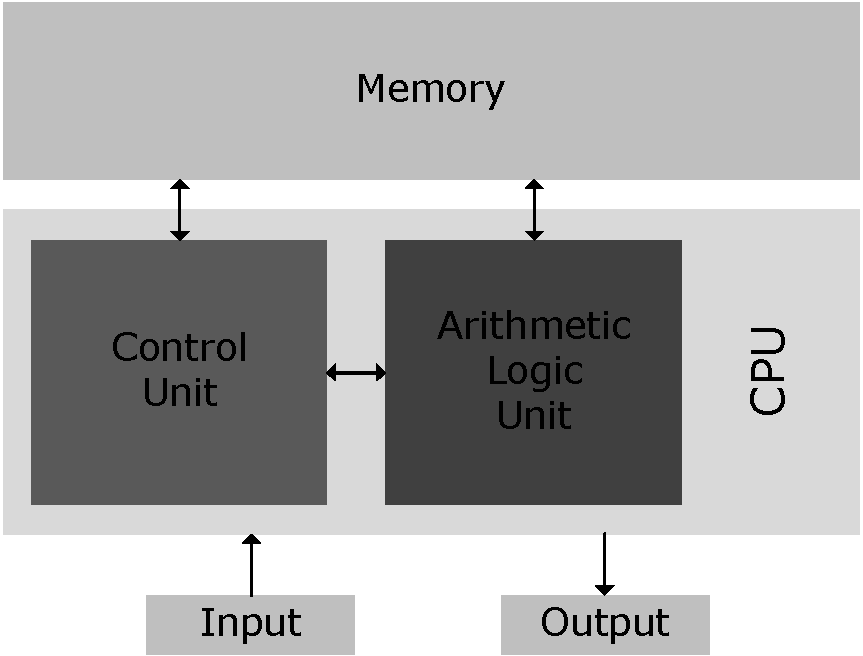
\includegraphics[width=0.6\columnwidth]{Chapter1/figures/vonneumann}
	\caption{Architecture de \emph{von Neumann}}
	\label{figvonneumann}
\end{figure}
Ce mod�le fut invent� par le math�maticien hongrois \emph{John von Neumann} qui a pos� les premi�res bases de la conception d'un ordinateur dans son papier de 1945 \cite{vonneumann}. A partir de ce moment tous les ordinateurs ont �t� con�us sur ces bases. L'architecture \emph{von Neumann} \ref{figvonneumann} est constitu�e de 4 composants principaux: une m�moire, une unit� de contr�le, une unit� arithm�tique et logique(\emph{ALU}) des Entr�es/Sorties (\emph{I/O}). La m�moire � acc�s al�atoire (\emph{RAM}) en lecture/�criture est utilis�e pour stocker les instructions ainsi que les donn�es. L'unit� de contr�le va chercher les instructions ou les donn�es de la m�moire, d�code les instructions et coordonne s�quentiellement les op�rations afin d'accomplir la t�che programm�e. L'ALU effectue les op�rations arithm�tiques de base. les I/O font l'interface avec l'utilisateur humain.
\subsubsection{Classification de Flynn des Machines Parall�les}
Il existe plusieurs mani�res de classer les machines parall�les. Toutefois, il existe une classification qui est largement utilis�e depuis 1966 et qui est celle de Flynn \cite{flynn} (\emph{Flynn's Taxonomy}). Cette classification distingue les architectures parall�les selon deux param�tres ind�pendants qui sont les instructions et les donn�es : chacun de ces deux param�tres peut avoir deux �tats possibles \emph{Single} ou \emph{Multiple}. Ainsi le tableau \ref{flynn} illustre la classification de Flynn.
\begin{table}
\centering
\begin{tabular}{|c||c|}
\hline
\textbf{SISD} &  \textbf{SIMD} \\
\hline
Single Instruction Single Data& Single Instruction Multiple Data\\
\hline
\hline
\textbf{MISD} &  \textbf{MIMD} \\
\hline
Multiple Instruction Single Data& Multiple Instruction Multiple Data\\
\hline
\end{tabular}
\caption{Classification de Flynn des machines parall�les}
\label{flynn}
\end{table}

\paragraph{Single Instruction, Single Data (SISD)}
Une machine s�rie qui ne peut ex�cuter qu'un seul flux d'instruction en un cycle d'horloge \emph{CPU}. De plus, un seul flux de donn�es est utilis� comme entr�e en un cycle d'horloge. L'ex�cution du programme y est d�terministe et il constitue le type de machines � la fois le plus ancien est le plus r�pandu de nos jours.
\paragraph{Single Instruction, Multiple Data (SIMD)}
C'est un type de machines parall�les dont les processeurs ex�cutent la m�me instruction en un cycle d'horloge donn�. Cependant, chaque unit� de traitement peut op�rer sur un �l�ment de donn�es diff�rent. Ce type de machines est bien taill� pour des probl�mes r�guliers tels que le traitement d'images et le rendu graphique. L'ex�cution des programme y est synchrone et d�terministe. Deux variantes de ces machines existent : 
\begin{itemize}
\item Processor Arrays: Connection Machine CM-2, MasPar MP-1 \& MP-2, ILLIAC IV
\item Vector Pipelines: IBM 9000, Cray X-MP, Y-MP \& C90, Fujitsu VP, NEC SX-2, Hitachi S820, ETA10 
\end{itemize}
De plus, la majorit� des processeurs des stations de travail actuelles et des unit�s de traitement graphiques, comportent une unit� de traitement sp�cialis�e SIMD, on parle alors de \emph{SWAR} (\emph{SIMD Within A Register}).

\paragraph{Multiple Instruction, Single Data (MISD)}
Un seul flux de donn�es alimente plusieurs unit�s de traitement et chaque unit� de traitement op�re sur les donn�es de mani�re ind�pendante gr�ce � un flot d'instructions ind�pendants. 
\paragraph{Multiple Instruction, Multiple Data (MIMD)}
C'est actuellement le type le plus commun de machines parall�les. Chaque processeur de ces machines peut ex�cuter un flux d'instructions diff�rent et peut op�rer sur un flux de donn�es diff�rent. L'ex�cution peut �tre synchrone ou asynchrone, d�terministe ou non-d�terministe. On peut citer les \emph{Supercomputers} actuels, les clusters de machines parall�les mis en r�seau, les grilles de calculs, les multi-processeurs SMP (Symetric Multi-Processor) et les processeur multi-core. De plus, plusieurs de ces machines contiennent des unit�s de traitement SIMD.

\subsection{Architectures M�moire des Machines Parall�les}
Dans la suite nous donnons une classification des machines parall�les selon le type de leur hi�rarchie m�moire. Cette classification permet d'une part de distinguer les machines parall�les d'un autre point de vue que celui du CPU et permet �galement de mieux comprendre les motivations des mod�les de programmation pour les machines parall�les.
\subsubsection{Les Machines Parall�les � M�moire Partag�e}
Il existe plusieurs variantes de ces machines mais toutes partagent une propri�t� commune qui est la capacit� de tous les processeurs d'acc�der toute la m�moire comme un espace d'adressage global. Ainsi, plusieurs processeurs peuvent op�rer d'une mani�re ind�pendante mais partagent la m�me ressource m�moire. Un changement op�r� par un processeurs dans un emplacement m�moire est visible � tous les autres processeurs. Cette classe de machine peut �tre divis�e en deux sous-classes bas�es sur les temps d'acc�s � la m�moire : UMA et NUMA.
\paragraph{Uniform Memory Access (UMA)}
\begin{figure}[!htb]
	\centering
	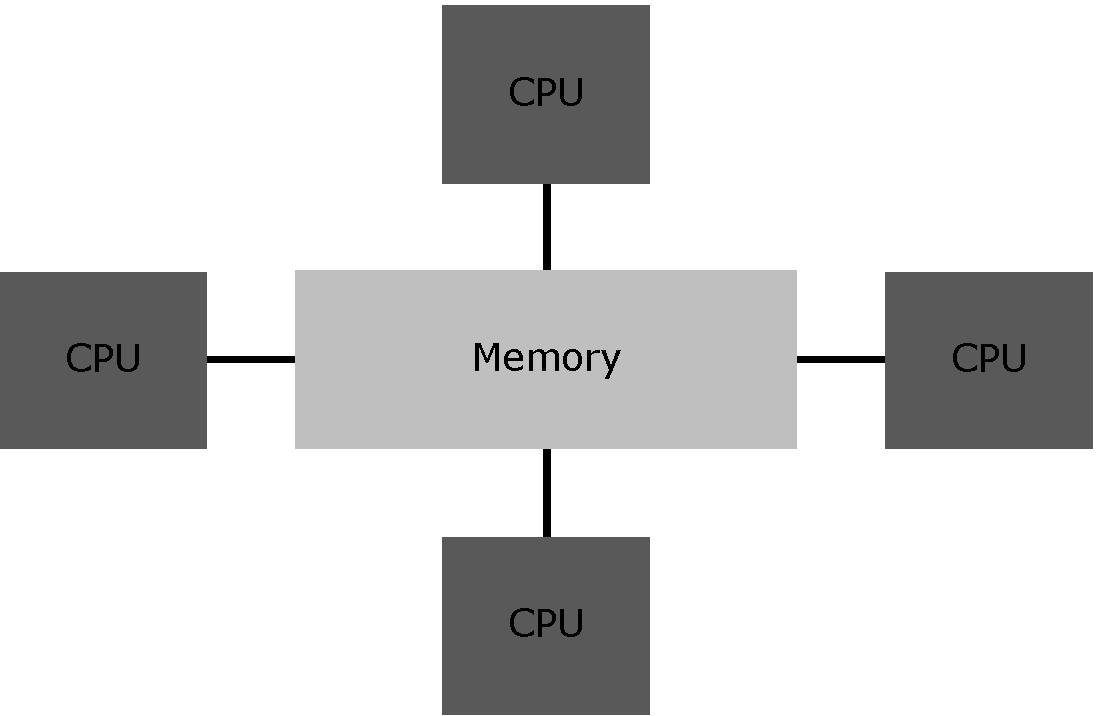
\includegraphics[width=0.7\columnwidth]{Chapter1/figures/SMUMA}
	\caption{Machine Parall�le � M�moire Partag�e UMA}
	\label{figSMUMA}
\end{figure}
Ce sont principalement les machines de type SMP qui poss�dent plusieurs processeurs identiques et qui peuvent acc�der de mani�re �gale et en un temps identique � la m�moire. Elles sont parfois appel�es CC-UMA - Cache Coherent UMA. La coh�rence de cache signifie que si un processeur met � jour un emplacement de la m�moire tous les autres processeurs sont au courant de ce changement. Cette fonctionnalit� est assur�e au niveau du \emph{hardware}.
\paragraph{Non-Uniform Memory Access (NUMA)}
\begin{figure}[!htb]
	\centering
	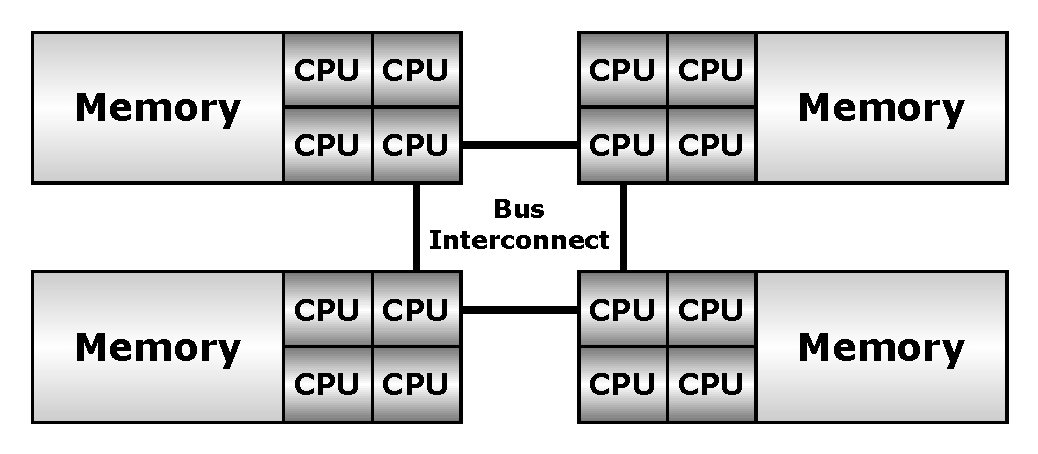
\includegraphics[width=0.7\columnwidth]{Chapter1/figures/SMNUMA}
	\caption{Machine Parall�le � M�moire Partag�e NUMA}
	\label{figSMNUMA}
\end{figure}
Ce type de machines est souvent con�u en connectant deux ou plusieurs SMPs. Un SMP peut avoir un acc�s direct � la m�moire d'un autre SMP. Le temps d'acc�s � une m�moire donn�e n'est pas �gal pour tous les processeurs et lorsque un noeud est travers� l'acc�s est plus lent. Si la coh�rence de cache est garantie on parle alors de CC-NUMA.

\paragraph{Avantages et Incov�nients}
Parmi les avantages de ce type d'architectures m�moire est une perspective simplifi�e de la m�moire du point de vue du programmeur. Le partage des donn�es entre les t�ches est � la fois rapide et uniforme. Le premier inconv�nient est le manque de mis � l'�chelle (\emph{scalability}) entre la m�moire et les CPUs. Le fait d'augmenter le nombre de CPUs augmente le trafic sur le bus m�moire et provoque un goulot d'�tranglement et la gestion de la coh�rence devient de plus en plus complexe. Le programmeur est responsable de la synchronisation des t�ches qui garantit un acc�s correcte � la m�moire globale. Par cons�quent, la conception de machine parall�les � m�moire partag�e avec de plus en plus de processeurs devient difficile et co�teux. 
\subsubsection{Les Machines Parall�les � M�moire Distribu�e}
\begin{figure}[!htb]
	\centering
	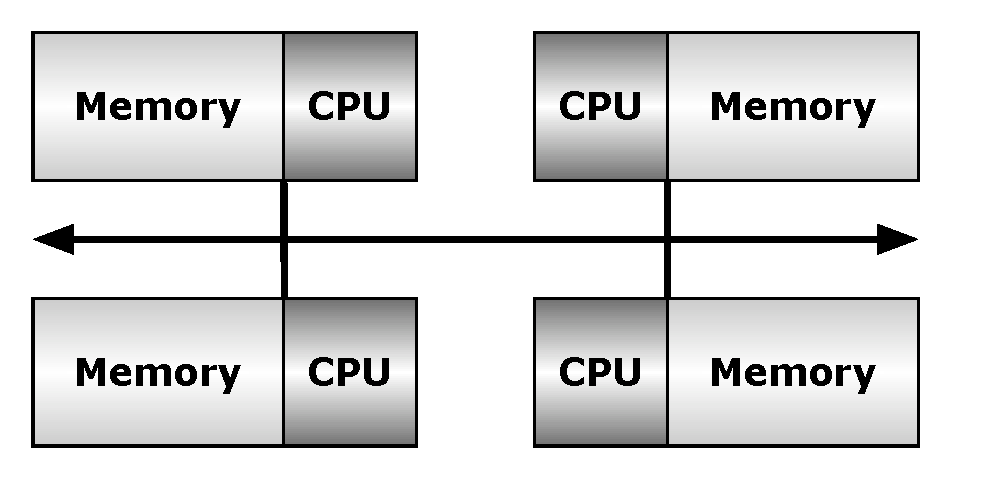
\includegraphics[width=0.7\columnwidth]{Chapter1/Figures/DMEM}
	\caption{Machine Parall�le � M�moire Distribu�e}
	\label{figDMEM}
\end{figure}
Comme les machines � m�moire partag�e, les machines � m�moire distribu�e varient mais elles partagent tout de m�me un point commun : elles requi�rent un r�seau de communication pour connecter la m�moire inter-processeurs. Les diff�rents processeurs poss�dent leur propre m�moire locale. Les adresses m�moire d'un processeur donn�e ne correspondent pas � celles d'un autre et par cons�quent le concept de m�moire globale n'existe pas. Puisque chaque processeur poss�de sa propre m�moire priv�e il op�re de mani�re ind�pendante. En effet, chaque changement op�r� sur sa m�moire locale n'as aucun effet sur la m�moire des autres processeurs ce qui exclue le concept de coh�rence de cache. Lorsqu'un processeur � besoin des donn�es contenues dans la m�moire d'un autre processeur, le programmeur est en charge de d�finir quand et comment les donn�es sont transf�r�es. Ce dernier est aussi responsable de la synchronisation.  
\paragraph{Avantages et Incov�nients}
L'avantage majeur de ce type d'architectures est le fait que la m�moire soit \emph{scalable} avec le nombre de processeurs. En effet, la taille de la m�moire croit proportionnellement avec le nombre de processeurs. Chaque processeur peut aussi acc�der rapidement � sa m�moire locale sans interf�rence et sans engendrer de surcout du au maintien de la coh�rence de cache. Le principal inconv�nient de ce type d'architectures m�moire et la gestion explicite par le logiciel des communications entre les processeurs. Les acc�s � la m�moire se font souvent � des temps non-uniformes et la pr�sence de plusieurs espaces d'adressage rend complexe l'adaptation de programmes �crits pour une m�moire partag�e.
\subsubsection{Les Machines Parall�les � M�moire Hybride}
\begin{figure}[!htb]
	\centering
	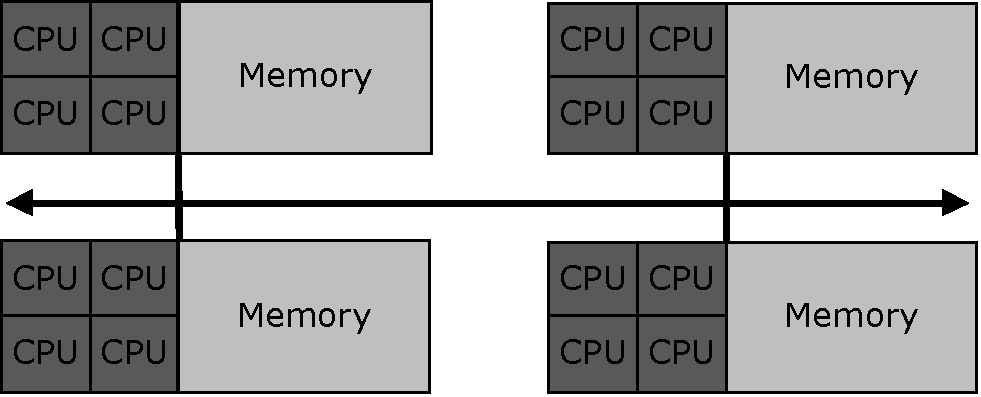
\includegraphics[width=0.7\columnwidth]{Chapter1/figures/HMEM}
	\caption{Machine Parall�le � M�moire Hybride}
	\label{figHMEM}
\end{figure}
Les machines les plus rapides du monde emploient des architectures m�moire dites hybrides qui regroupent les deux types pr�c�dents: partag�e et distribu�e. La composante m�moire partag�e est souvent une machine SMP. La composante distribu�e quant � elle consiste en la mise en r�seau de plusieurs machines SMP. Les diff�rents SMPs ne peuvent adresser que leur propre m�moire et le transfert de donn�es entre deux SMPs requiert des communications au travers du r�seau. Selon le niveau dans lequel on se trouve, ce type de machines poss�de les inconv�nients et avantages des deux pr�c�dentes architectures m�moire.
\subsection{Mod�les de Programmation Parall�le}
Il existe plusieurs mod�les de programmation pour les machines parall�les. Ces mod�les existent � un niveau d'abstraction au dessus de l'architecture mat�rielle et de celle de la m�moire. M�me si � premi�re vue les mod�les de programmation sont intimement li�s � l'architecture de la machine ils sont suppos�s pouvoir �tre impl�ment�s sur n'importe quelle machine parall�le quelqu'en soient les caract�ristiques. Il n'existe pas de mod�le de programmation id�al mais certains mod�les de programmation sont bien adapt�s pour une application donn�es sur une machine donn�e. Dans la suite nous d�crivons les principaux mod�les de programmation parall�les.
\subsubsection{Le Mod�le \emph{Shared Memory}}
Dans ce mod�le de programmation les t�ches partagent un espace d'adressage commun sur lequel ils peuvent lire et �crire des donn�es de mani�re asynchrone. Plusieurs m�canismes, tels que les \emph{locks} et les s�maphores peuvent �tre utilis�s pour contr�ler l'acc�s � la m�moire partag�e. Ce mod�le de programmation est simplifi� du point de vue de l'utilisateur car il n'y a pas de notion d'appartenance des donn�es � une t�che ce qui �vite les communication explicite pour transf�rer des donn�es d'une t�che � une autre. Toutefois, en terme de performances ce dernier point constitue in inconv�nient car il engendre un surcout d'acc�s � la m�moire de rafraichissement de cache et de trafic sur le bus lorsque plusieurs processeurs utilisent les m�mes donn�es.
Les impl�mentations de ce mod�le sur les machines � m�moire partag�s se r�sument au compilateur natif qui traduit les variables du programme en adresse m�moire globales. Il n'existe cependant pas d'impl�mentation de ce mod�le sur des machines � m�moire distribu�e.
\subsubsection{Le Mod�le de Programmation par \emph{Threads}}
Dans le mod�le de programmation par threads, un seul \emph{process} peut avoir des chemins d'ex�cution multiples et concurrents. On peut assimiler ce concepts � un programme principal qui inclue un certain nombre de sous-routines. Le programme principal est ordonnanc� pour �tre ex�cut� par les syst�me d'exploitation, et il acqui�rent toutes les ressources syst�me n�cessaires � son ex�cution. Il effectue alors un ensemble d'instructions en s�rie et cr�e un certain nombres de t�ches (\emph{threads}) qui peuvent �tre ordonnanc�es et ex�cut�es par l'OS de mani�re concurrente. Chaque \emph{thread} poss�de ses donn�es locales mais partage �galement les ressources du programme principal avec les autres \emph{threads}. Chaque \emph{thread} poss�de un acc�s � la m�moire globale car il partage l'espace d'adressage du programme principal. La charge du travail d'un \emph{thread} peut �tre consid�r�e comme une sous-routine du programme principal mais qui peut s'ex�cuter en parall�le d'un autre \emph{thread}. Les \emph{threads} communiquent entre eux via la m�moire globale ce qui n�cessite des op�rations de synchronisation afin de garantir l'exclusivit� de l'acc�s � un emplacement donn�e � un instant donn� pour un seul \emph{thread}. Les \emph{threads} on une dur�e de vie variable et peuvent �tre cr�es et d�truits tout au long du d�roulement du programme. Le mod�le de programmation par \emph{thread} est souvent associ� avec les machines � m�moire partag�e. Les impl�mentations des \emph{threads} comportent en g�n�ral une librairie de fonctions ou alors une s�rie de directives enfouis dans le code parall�le. Dans les deux cas l'utilisateur est responsable de la d�finition du parall�lisme. Il existe plusieurs impl�mentations des \emph{threads}, et la plupart des  constructeurs ont d�velopp� leur propre version ce qui a affect� la portabilit� des codes parall�les. Cependant, un effort de standardisation � donn� naissance � deux impl�mentations qui sont devenues le standard de nos jours.
\paragraph{Les \emph{Threads} POSIX}
Ils sont bas� sur une librairie de programmation parall�le et sp�cifi�es par le standard \emph{IEEE POSIX 1003.1c standard (1995)} \cite{pthreads_std}. Ils sont impl�ment�s uniquement en langage C et plus connus sous le nom de \emph{Pthreads}. Le parall�lisme y est explicite et l'interface bas-niveau force le programmeur � donner beaucoup d'attention au d�tails.
\paragraph{OpenMP}
C'est un mod�le de programmation bas� sur des directives de compilation et peut �tre directement utilis� sur du code s�rie. Ce standard � �t� d�fini par un consortium de vendeurs de processeurs et de logiciel. L'API Fortran � �t� d�livr�e en 1997 alors que l'API C/C++ ne l'a �t� qu'une ann�e plus tard. C'est une API portable et multi-plateforme et est tr�s simple d'utilisation.
\subsubsection{Le Mod�le \emph{Message Passing}}
Dans ce mod�le, la programmation parall�le se fait par passage de messages. Un ensemble de t�che utilisent leur propre m�moire locale durant le calcul. Plusieurs t�ches peuvent r�sider sur la m�me machine physique ou alors sur un nombre arbitraire de machines. Les t�ches �changent des donn�es au travers des communications en envoyant et recevant des messages. Les transferts de donn�es requi�rent des op�rations coop�ratives pour �tre effectu�es par chaque \emph{process}. Par exemple, une op�ration \emph{send} doit avoir une op�ration sym�trique \emph{receive}. Les impl�mentations du \emph{Message Passing} prennent la forme d'une librairie de sous-routines et le programmeur est responsable de la d�termination du parall�lisme. Comme pour toute librairie, plusieurs versions ont �t� d�velopp�es, ce qui a provoqu� des probl�mes de compatibilit�. En 1992 le \emph{MPI Forum} a vu le jour dans le but de standardiser les impl�mentations du \emph{Message Passing} et a d�livr� deux standard MPI \cite{mpistand} en 1994 et MPI-2 en 1996. Des nos jours MPI est le mod�le de programmation le plus utilis� pour le \emph{Message Passing}. Dans les impl�mentations MPI sur des architectures � m�moire partag�e les communications r�seaux sont tout simplement remplac�es par des copies m�moire.

\subsubsection{Le Mod�le \emph{Data Parallel}}
Ce mod�le est bas� sur le parall�lisme de donn�es qui concentre le travail en parall�le sur un ensemble de donn�es sur un tableau � une ou plusieurs dimensions. Un ensemble de t�ches travaillent collectivement sur la m�me structure de donn�es mais chaque t�ches op�re sur une partition diff�rente de cette structure. Les t�ches effectuent toutes la m�me op�ration sur leur partition de donn�es. Sur les architectures � m�moire partag�e toutes les t�ches peuvent avoir acc�s � la structure de donn�es via la m�moire globale. Par contre lorsque l'architecture m�moire est distribu�e les donn�es sont divis�es en morceaux qui r�sident dans la m�moire locale de chaque t�che. La programmation avec ce mod�le se fait en g�n�ral en �crivant du code avec des constructions de parall�lisme de donn�es. Ces derni�res peuvent avoir la forme d'appel � des fonction d'une librairie ou � des directives reconnues par un compilateur \emph{data parallel}. Les impl�mentation de ce mod�le sont souvent des extensions ou de nouveaux compilateurs on peut citer les compilateur \texttt{Fortran} (\texttt{F90 et F95}) et leur extension High Performance Fortran (\emph{HPF}) qui supportent la programmation \emph{data parallel}. \emph{HPF} inclue des directives qui contr�lent la distribution des donn�es, des assertions qui peuvent am�liorer l'optimisation du code g�n�r� ainsi que des construction \emph{data parallel}. Les impl�mentations sur les architectures m�moire distribu�es de ce mod�le sont sous forme d'une compilateur qui convertit le code standard en code \emph{Message Passing} (MPI) qui distribue les donn�es sur les diff�rents processeurs et tout cela de mani�re transparent du point de vue de l'utilisateur.

\subsubsection{Autres Mod�les}
D'autres mod�les existent et existeront dans le futur proche en plus de ceux mentionn�s auparavant. On peut en mentionner trois :
\paragraph{Mod�le Hybride}
Dans ce mod�le deux ou plusieurs mod�les sont combin�s. On peut citer par exemple la combinaison de \emph{MPI} avec les \emph{Pthreads} ou avec \emph{OpenMP}. Ainsi, diff�rents niveaux de parall�lisme sont g�r�s, par exemple un r�seau de SMPs. On peut citer �galement la combinaison de \emph{HPF} avec \emph{MPI} pour le m�me type de configuration.
\paragraph{Mod�le Single Program Multiple Data}
Le mod�le \emph{SPMD} est un mod�le haut niveau qui peut �tre construit sur la base d'une combinaison des mod�les cit�s pr�c�demment. Un seul programme est ex�cut� par toutes les t�che simultan�ment. A n'importe quel instant les t�chent peuvent ex�cuter des instructions diff�rentes ou similaires du m�me programme.Un programme \emph{SPMD} peut toutefois contenir des branchement qui permettent � une t�che de n'ex�cuter qu'une portion du code et toutes les t�ches peuvent utiliser diff�rentes donn�es.
\paragraph{Mod�le Multiple Program Multiple Data}
Tout comme le mod�le \emph{SPMD}, le mod�le \emph{MPMD} est haut-niveau et peut englober l'ensemble des mod�les cit�es pr�c�demment. Les programmes \emph{MPMD} ont typiquement plusieurs objets ex�cutables. Lors de l'ex�cution parall�le du programme une t�che peut ex�cuter le m�me programme ou un programme diff�rent et toutes les t�ches peuvent utiliser des donn�es diff�rentes.

\section{Parall�lisation}
Les architectures parall�les et les mod�les de programmation associ�s �tant d�finis. La question qui se pose alors est celle du choix � la fois de l'architecture et du mod�le de programmation ad�quats pour la mise en oeuvre d'une application parall�le donn�e. L'efficacit� des outils automatiques de parall�lisation d�pend souvent de plusieurs facteurs, parmi lesquelles : les caract�ristiques de l'architecture mat�rielle et de la hi�rarchie m�moire ainsi que la nature des algorithmes qui forment l'application � parall�liser.  L'utilisation d'outils automatiques n'est pas toujours efficace, il est alors parfois n�cessaire de g�rer manuellement le parall�lisme et les optimisations qui lui sont associ�es. Deux choix se pr�sentent alors :
\subsection{Parall�lisation Manuelle}
Elle permet un contr�le pr�cis de la performance, et une grande flexibilit� en termes de sch�ma de parall�lisation possible (diff�rents mod�les de calcul). Par contre, les temps de d�veloppement sont importants, que cela soit pour la mise en �uvre, le d�bogage ou la maintenance de l'application. Les erreurs sont parfois tr�s difficiles � trouver, et le processus d'optimisation est souvent it�ratif.

\subsection{Parall�lisation Automatique}
L'automatisation du processus de parall�lisation de code est un probl�me ouvert, et les efforts effectu�s en la mati�re sont de plus en plus nombreux, en particulier avec l'av�nement des nouvelles architectures parall�les et leur d�mocratisation. On peut trouver deux formes d'outils automatiques de parall�lisation. Certains outils sont enti�rement automatiques : ils prennent en entr�e un code source s�rie et d�tectent automatiquement le parall�lisme potentiel ils g�n�rent en suite le code parall�le correspondant. D'autres outils sont semi-automatiques car l'utilisateur indique les portions de codes parall�lisables, c'est le cas par exemple d'OpenMP via les directives de compilation.
L'avantage des approches automatiques est avant tout la rapidit� de mise en �uvre d'une solution � base de calcul parall�le, d'autant plus que dans la majorit� des cas le code original est directement utilisable. Par contre, le contr�le est beaucoup moins pr�cis qu'avec une version enti�rement manuelle. Il peut y avoir par exemple des erreurs dans les r�sultats de calcul. De plus, les mod�les de programmation dans ce cas ne permettent pas une grande flexibilit� dans le choix des sch�mas de parall�lisation. Dans certains cas le gain de performance peut �tre m�diocre, et on peut m�me observer une baisse de performances par rapport � la version originale. Enfin, ce genre d'outils n'est g�n�ralement efficace que sur des portions de code facilement utilisable comme les boucles. 
Dans la suite nous allons pr�senter les diff�rentes �tapes de mise en �uvre d'un code parall�le manuellement, les �tapes en question vont de la d�termination de l'opportunit� de parall�lisation jusqu'� la mise en ouvre et l'�valuation du gain ainsi obtenu.



%Le traitement d'images est une discipline du traitement du signal dont l'entr�e est une image. Les techniques de traitement du signal sont appliqu�es � un signal de 2 dimensions pour donner en sortie soit une image, soit une certaine caract�ristique de l'image. Dans notre cas on s'int�resse au traitement d'images de bas niveau, ou les op�rateurs sont souvent des op�rateurs point-�-point ou des noyaux de convolution. Ce type de calcul est bien adapt� aux machines parall�les car il n'y a g�n�ralement pas de d�pendances de donn�es et les algorithmes de bas-niveau sont majoritairement des op�rations de calcul pur. Toutefois, pour des applications de moyen-niveau, par exemple la segmentation, il existe une forte d�pendance de donn�es et les algorithmes sont souvent des imbrications de structures conditions. Ceci rend la t�che de parall�lisation pour ce types d'algorithmes fastidieuse, et les acc�l�rations sont souvent m�diocres en comparaison avec l'effort fourni pour l'adaptation de l'algorithme s�rie. La conception d'une version parall�le d'un algorithme devient une t�che fastidieuse et qui d�pend de plusieurs facteurs. Il est alors important d'accorder de l'importance � plusieurs aspects d�terminants pour la performance.
%\subsection{Le Partitionnement}
%La premi�re t�che lors de la parall�lisation d'une application de traitement d'image est le choix du type partitionnement � adopter. Ce principe prend �a source du fait qu'il y a plusieurs ressources et que le but est de repartir la charge de travail sur ces ressources sous formes de morceaux qui peuvent �tre distribu�s sur plusieurs t�ches. Il existe deux m�thodes basiques pour le partitionnement la d�composition de domaine (\emph{domain decomposition}) et la d�composition fonctionnelle (\emph{functionnal decomposition})
%\subsubsection{D�composition de Domaine}
%\begin{figure}[htb]
%	\centering
%	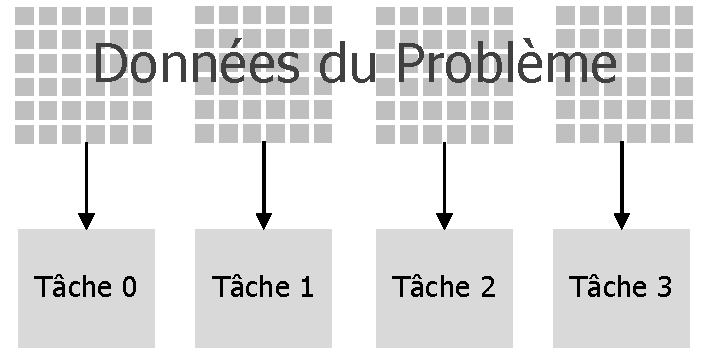
\includegraphics[width=0.8\columnwidth]{Chapter1/figures/domaindecomp}
%	\caption{Partitonnement par d�composition du domaine}
%	\label{figdomain}
%\end{figure}

%Dans ce type de partitionnement, les donn�es associ�es au probl�me sont d�compos�es. Chaque t�che parall�le travaille donc sur une portion des donn�es. Il existe alors plusieurs mani�res de d�composer les donn�es. En traitement d'images, les donn�es sont en 2 dimensions les d�compositions possibles sont illustr�es en figure \ref{decomp2D}.

%\begin{figure}[htb]
%	\centering
%	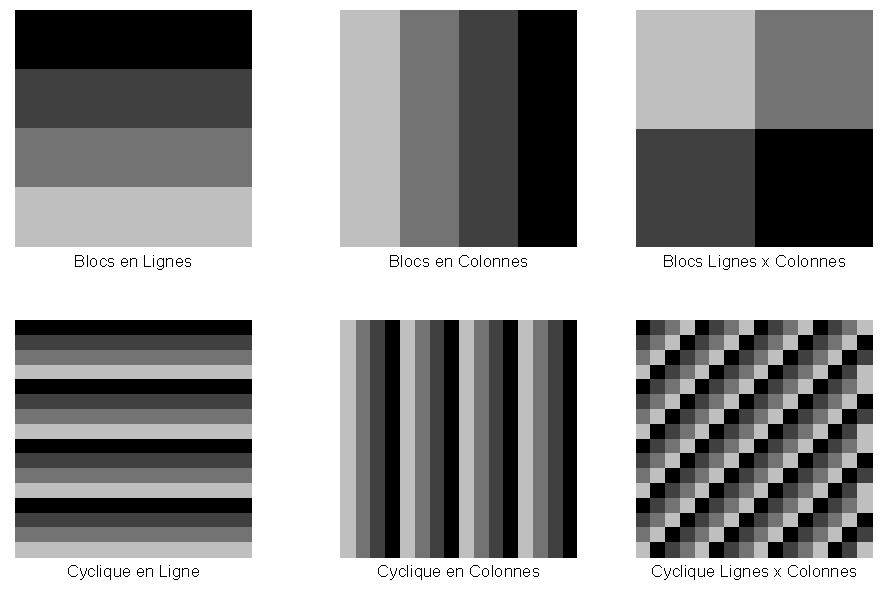
\includegraphics[width=0.8\columnwidth]{Chapter1/figures/decomp2D}
%	\caption{Partitonnement par d�composition du domaine en traitement d'images}
%	\label{decomp2D}
%\end{figure}






%\begin{quote}
%\emph{"I think games are an interesting application area, but quite clearly, Cell is not just for games.  There are many other areas it can be used.  Games are the thing that inspired us to do it.}\\
%Peter Hofstee, chief architect of the Cell processor
%\end{quote}
\indent Le processeur Cell\cite{Cell_Johns_2007} est une architecture unique en son genre car elle renferme une multitude de dispositifs d�di�s au calcul haute-performance. Son architecture parall�le � plusieurs niveaux permet aux utilisateurs aguerris d'atteindre des performances jusque l� r�serv�es aux seuls clusters de machines et utilisant des paradigmes de haut niveau tels que le \emph{message-passing}. En ce sens l'architecture du Cell, destin�e initialement au domaine des jeux vid�os, a trouv� d'autres d�bouch�s notamment dans le calcul scientifique au sens large.\\
\indent Le Cell est compos� d'un processeur PowerPC classique nomm� PPE (Power Processor Element) et de huit unit�s de calcul acc�l�ratrices appel�es SPE (\emph{Synergestic Processor Element}). Ces unit�s de calcul sont reli�es par un bus interne qui permet �galement l'acc�s � la m�moire principale (\emph{Main Storage}), ainsi qu'�  d'autres p�riph�riques externes. Le processeur Cell est consid�r� comme un processeur h�t�rog�ne car il comporte deux types d'architectures diff�rentes : celle du PPE qui n'est autre qu'une d�clinaison du PowerPC 970, et celle des SPEs qui sont des unit�s SIMD acc�l�ratrices sp�cialis�es dans des traitements contenant un flot de donn�es important comme le multim�dia par exemple. Le jeu d'instructions vectorielles des SPE est tr�s proche d'Altivec\cite{altivec_2000}, pr�sent sur les architectures de type PowerPC \\
\section{Vue g�n�rale}
\begin{figure}[!htbf]
	\centering
	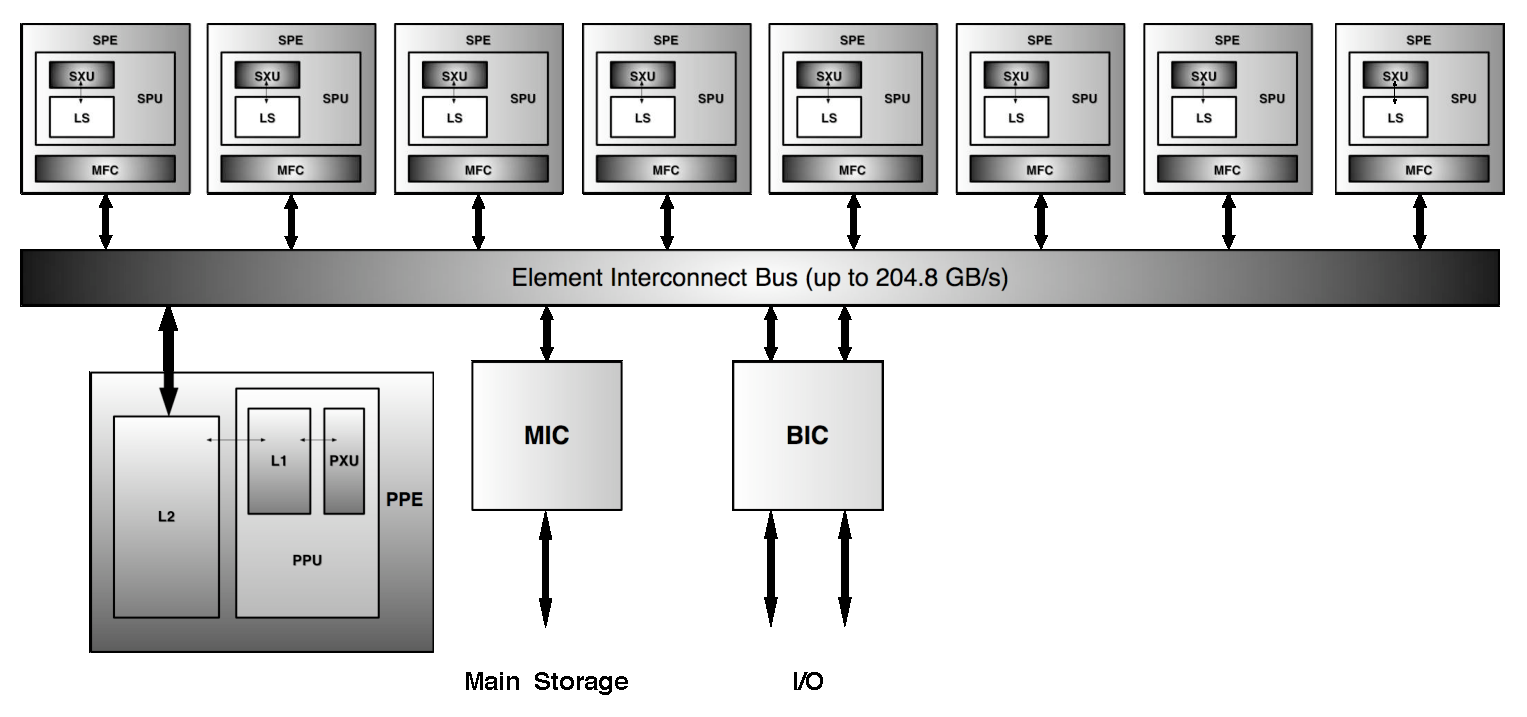
\includegraphics[scale =0.65]{Chapter2/figures/cell_fig01_bw}
	\caption{Vue d'ensemble de l'architecture h�t�rog�ne du processeur Cell}
  \label{cell_fig1}
\end{figure}
Le processeur Cell est la premi�re impl�mentation de l'architecture \emph{Cell Broadband Engine} (CBEA), qui est enti�rement compatible avec l'architecture \emph{PowerPC} 64-bit. Ce processeur � �t� initialement con�u pour la console de jeux \emph{PlayStation 3} mais ses performances hors normes ont tr�s vite fait de lui un bon candidat pour d'autres domaines d'applications qui requi�rent une grande puissance de calcul, comme le traitement du signal et des images.\\
Le processeur Cell est une machine multi-coeurs h�t�rog�ne, capable d'effectuer une quantit� de calcul en virgule flottante consid�rable, sur des donn�es occupant une large bande-passante. Il est compos� d'un processeur 64-bit appel� \emph{Power Processor Element} (PPE), huit co-processeurs sp�cialis�s appel�s \emph{Synergistic Processor Element} (SPE), un contr�leur m�moire haute-vitesse et une interface de bus � large bande-passante. Le tout int�gr� sur une seule et m�me puce.\\
Le PPE et les SPEs communiquent par le biais d'un bus interne de communication tr�s rapide appel� \emph{Element Interconnect Bus} (EIB) (Fig. \ref{cell_fig1}). Avec une fr�quence d'horloge de 3.2 GHz, le processeur Cell peut atteindre th�oriquement une performance cr�te de 204.8 GFlop/s en flottants simple-pr�cision (32 bits) et 14.6 GFlop/s en flottants double-pr�cision (64 bits). Il est important de noter que sur la premi�re version du Cell, le d�bit des instructions arithm�tiques en double-pr�cision �tait d'une instruction tous les 7 cycles ce qui explique les 14.6 GFlop/s. Ce d�bit a �t� am�lior� pour atteindre une instruction par cycle sur la derni�re g�n�ration \emph{PowerXCell 8i}, ce qui correspond  � une puissance de calcul de 102.4 GFlop/s. \\
%Le bus interne supporte une bande passante qui peut aller jusqu'� 204.8 Go/s pour les transferts internes � la puce (impliquant le PPE, les SPEs, la m�moire et les contr�leurs I/O). le contr�leur m�moire: \emph{Memory Interface Controller} (MIC) fournit une bande-passante de 25.6 Gbytes/s vers la m�moire principale. Le contr�leur I/O quand � lui fournit 25 Gbytes/s en entr�e et 35 Gbytes/s en sortie.\\
%Le r�le du PPE est celui d'un chef d'orchestre. Il prend en charge l'OS (\emph{Operating System}) et coordonne les SPEs. Au niveau de l'architecture c'est un \emph{PowerPC} 64-bit classique avec une extension SIMD, un cache L1 de 32 Ko (donn�es et instructions) et un cache L2 de 512 KB. C'est un processeur � ex�cution dans l'ordre (\emph{in-order execution processor}), il supporte le \emph{dual-issue} (parall�lisme d'instructions) ainsi que le multi-threading d'ordre 2 (parall�lisme de t�ches).\\
%Chaque SPE est compos� d'une SPU (\emph{Synergistic Processor Unit}) et d'un MFC (\emph{Memory Flow Controller}). Le MFC contient � son tour un contr�leur DMA (\emph{Direct Access Memory}), une unit� de gestion de la m�moire (MMU), une unit� interface de bus, et une unit� atomique pour la synchronisation avec les autres SPEs et le PPE. Le SPU est un processeur de type RISC avec un jeu d'instructions et une micro-architecture con�us pour les applications flot de donn�es haute-performance ou de calcul intensif. Le SPU inclut une m�moire locale de 256 Ko qui contient les donn�es et les instructions. Le SPU ne peut pas acc�der directement � la m�moire principale mais par le biais de commandes DMA via le MFC qui permettent de lire et d'�crire dans la m�moire principale. Les deux unit�s MFC et SPU sont ind�pendantes ce qui permet l'ex�cution des t�ches de calcul et de transferts en parall�le sur le SPE.\\
%l n'existe pas de m�canisme hardware tel que la m�moire cache pour la gestion automatique des m�moires locales, et celles-ci doivent �tre g�r�es par le software. Le MFC effectue des commandes DMA pour transf�rer entre la m�moire centrale et les m�moires locales. Les instructions DMA pointent des emplacements de la m�moire centrale en utilisant des adresses virtuelles compatibles \emph{PowerPC}. Les commandes DMA peuvent transf�rer des donn�es � partir de n'importe quel emplacement li� au bus d'interconnexion (m�moire principale, la m�moire locale d'un autre SPE, ou un p�riph�rique I/O). Des transferts SPE vers SPE en parall�le sont faisables � raison de 16 \emph{bytes} par cycle d'horloge SPE, tandis que la bande-passante de la m�moire centrale est de 25.6 Gbytes/s pour le processeur entier.\\
%Chaque SPU contient 128 registres SIMD de taille 128-bits. Cette quantit� importante de registres facilite l'ordonnancement efficace des instructions ainsi que d'autres optimisations comme le d�roulage de boucle (loop-unrolling).\\
%Toutes les instructions SIMD sont des instructions que le pipeline peut ex�cuter � 4 granularit�s: 16 entiers 8-bit, 8 entiers 16-bit, 4 entiers 32-bits ou flottants simple-pr�cision. Le processeur SPU est un processeur � ex�cution dans l'ordre (\emph{in-order-execution processor}), il poss�de deux pipelines d'instructions connus sous les d�nominations pair (\emph{even}) et impair (\emph{odd}).\\
%Les instructions flottantes et enti�res sont dans le pipeline \emph{even} alors que le reste est dans le pipeline \emph{odd}. Chaque SPU peut lancer et compl�ter jusqu'� deux instructions par cycle, une par pipeline. Toutes les instructions flottantes en simple-pr�cision peuvent �tre lanc�es en un cycle d'horloge du processeur. Par contre les instructions flottantes en double-pr�cision ne sont pipelin�es que partiellement, il en r�sulte un d�bit d'ex�cution moindre (deux instructions double-pr�cision tous les 7 cycles d'horloge SPU).\\
%Si l'on prend une instruction de multiplication accumulation en flottant simple-pr�cision (qui compte pour deux op�rations) les 8 SPEs peuvent ex�cuter un total de 64 op�rations par cycle \cite{kahle_2005}.\\

\subsection{Le PPE:  Power Processor Element}
Le PPE est un processeur 64 bits compatible avec l'architecture POWER\cite{ibm_power}, optimis� au niveau de l'efficacit� �nerg�tique\cite{Cell_Hofstee_2005}. La profondeur de pipeline du PPE est de 23 �tages\cite{Cell_Kahle_2005}, chiffre qui peut paraitre faible par rapport au pr�c�dentes architectures PowerPC surtout quand on sait que la dur�e de l'�tage est r�duite d'un facteur 2. Le PPE est une architecture \emph{dual-issue} (deux instructions peuvent �tre lanc�es par cycle) qui ne r�ordonne pas dynamiquement les instructions  (ex�cution dans l'ordre). Les instructions arithm�tiques simples, s'ex�cutent et fournissent leur r�sultat en deux cycles. Les instructions de chargements (\texttt{LOAD}) s'ex�cutent �galement en deux cycles. Une instruction flottante en double pr�cision s'ex�cute en dix cycles. Le PPE supporte une hi�rarchie conventionnelle de caches, avec un cache L1 (de niveau 1) donn�es et instructions de 32 Ko, et un cache L2 de 512 Ko.\\
Le PPE peut lancer deux \emph{threads} simultan�ment et peut �tre vu comme un processeur double-coeur avec un flot de donn�es partag�, ceci donne l'impression au logiciel d'avoir deux unit�s de traitement distinctes. Les registres sont dupliqu�s mais pas les caches qui sont partag�s par les deux \emph{threads}. Les instructions provenant de deux \emph{threads} de calcul diff�rents sont entrelac�es afin d'optimiser l'utilisation de la fen�tre d'ex�cution.\\
Le processeur est compos� de trois unit�s : l'unit� d'instructions (UI) responsable du chargement, d�codage, branchements, ex�cution et compl�tion des instructions. Une unit� d'ex�cution des op�rations en arithm�tique point-fixe (XU) qui est �galement responsable des instructions \texttt{LOAD/STORE}. Et enfin l'unit� VSU qui ex�cute les instructions en virgule flottante ainsi que les instructions vectorielles. Les instructions SIMD dans le PPE sont celles des g�n�rations pr�c�dentes de PowerPC 970 et effectuent des op�rations sur des registres 128 bits de donn�es qui permettent un parall�lisme de 2, 4, 8 ou 16, selon le type de donn�es trait�.

\subsection{Les SPE (Synergistic Processing Element)}
Le SPE contient un jeu d'instructions nouveau mais qui n'est autre qu'une version r�duite du jeu d'instructions SIMD VMX, strictement �quivalent au jeu d'instructions Altivec cit� auparavant, mais optimis� au niveau de la consommation d'�nergie et des performances pour les applications de calcul intensif et de multimedia. Le SPE contient une m�moire locale de 256 Ko (\emph{scratchpad}) qui est une m�moire de donn�es et d'instructions. Les donn�es et les instructions sont transf�r�es de la m�moire centrale vers cette m�moire priv�e au travers de commandes DMA qui sont ex�cut�es par le MFC (Memory Flow Controller) qui est pr�sent dans chaque SPE. Chaque SPE peut supporter jusqu'� 16 commandes DMA en suspens. L'unit� DMA peut �tre programm�e de trois mani�res diff�rentes : 1) avec des instructions sur le SPE qui ins�rent des commandes DMA dans la file d'attente; 2) par la programmation de transferts permettant de faire des acc�s sur des zones non contigu�s de la  m�moire en utilisant une liste de DMA, ce qui permet de d�finir un ensemble de transferts contigus de tailles diff�rentes; 3) par l'insertion d'une commande DMA dans la file d'attente d'un autre processeur par les commandes de DMA-write.\\
Afin de faciliter la programmation et de permettre des transferts entre SPEs, les m�moires locales sont dupliqu�es en m�moire centrale. La pr�sence des m�moires locales introduit un autre niveau dans la hi�rarchie m�moire au-dessus des registres. Le temps d'acc�s � ces m�moires est de l'ordre du cycle ce qui en fait de bons candidats pour r�duire la latence d'acc�s � la m�moire centrale qui est de l'ordre du millier de cycles. De plus, le contr�leur DMA est ind�pendant de l'unit� de calcul ce qui donne un niveau de parall�lisme suppl�mentaire. La pr�sence de ces m�moires priv�es permet d'appliquer diff�rents mod�les de programmation sur le processeur Cell.\\
La m�moire locale est le composant le plus important en taille du SPE, et il �tait important de l'impl�menter de mani�re efficace. Une m�moire SRAM � un seul port est utilis�e pour r�duire la surface. En d�pit du fait que la m�moire locale doit arbitrer entre lectures/�critures DMA, chargements d'instructions, et  lecture/�criture m�moire, celle-ci a �t� con�ue avec de ports de lecture moyens (128-bits) et larges (128 octets) dans le but de toujours fournir la meilleure performance possible. Le port le plus large est utilis� pour les commandes DMA et le chargement d'instructions. Cela est d� au fait qu'une commande DMA de 128 octets requi�re 16 cycles d'horloge pour placer les donn�es sur le bus coh�rent du Cell, m�me lorsque les commandes DMA s'ex�cutent avec une bande passante maximale. Ainsi, 7 sur 8 cycles d'horloge restent disponibles pour les \texttt{LOAD}, \texttt{STORE} et les chargements d'instructions. De la m�me mani�re, les instructions sont charg�es par morceaux de 128 octets et la pression sur la m�moire locale est par cons�quent r�duite. La plus haute priorit� est donn�e aux commandes DMA, la seconde plus haute priorit� aux commandes \texttt{LOAD} et \texttt{STORE}, le chargement ou pr�-chargement des instructions n'est fait que lorsqu'il y a des cycles disponibles. Toutefois, une instruction qui force la disponibilit� d'une fen�tre d'ex�cution pour le chargement d'instructions existe.\\
Les unit�s d'ex�cution du SPE sont organis�es autour d'un flot de donn�es 128 bits. Un banc de 128 registres fournit assez d'entr�es pour permettre � un compilateur de r�organiser des groupes d'instructions afin de masquer la latence d'ex�cution des instructions. Il n'y a qu'un seul banc de registres et toutes les instructions sont SIMD 128 bits avec une largeur d'�l�ment diff�rente selon le type (2x64 bits, 4x32 bits, 8x16 bits, 16x8 bits et 128x 1 bit). Deux instructions sont lanc�es � chaque cycle :  une fen�tre d'ex�cution supporte les instructions en virgule fixe et flottante et l'autre ex�cute les instructions \texttt{LOAD} et \texttt{STORE}, les permutations, ainsi que les instructions de branchement. Les op�rations simples sur des entiers prennent deux cycles, les op�rations sur des flottants simple-pr�cision et les instructions \texttt{LOAD} prennent 6 cycles. Les instructions vectorielles en flottants double-pr�cision sont �galement support�es et leur d�bit maximal est d'une instruction tous les 7 cycles pour la premi�re g�n�ration du Cell, et 1 cycle pour la derni�re g�n�ration. Toutes les autres instructions sont enti�rement pipelin�es quelque soit la g�n�ration du processeur.\\
Afin de limiter la complexit� du mat�riel d�di� � la pr�diction de branchement, une pr�diction de branchement peut �tre fournie par le programmeur ou le compilateur. L'instruction de pr�diction de branchement informe le mat�riel de l'adresse cible du branchement � venir, et le mat�riel r�pond en pr�-chargeant au moins 17 instructions � partir de l'adresse cible de branchement. Une instruction de masque de s�lection par bits peut �galement �tre utilis�e afin d'�viter les branchements conditionnels dans le code. La surface d�di�e aux unit�s de contr�le ne repr�sente alors que 10 � 15 \% de la surface totale de 10 $mm^{2}$ du SPE. Le SPE ne dissipe que tr�s peu de \emph{Watts} tout en op�rant � une fr�quence de 3.2 GHz.
%L'ensemble des sp�cificit�s des SPEs cit�es auparavant rendent la programmation de ces derniers fastidieuse. Les instructions arithm�tiques des SPEs sont exclusivement vectorielles :  le calcul se fait forc�ment sur des registres de 128 bits et l'acc�s � la m�moire doit se faire avec un alignement multiple de 16 octets. Le jeu d'instructions est assez restreint compar� � ses pr�d�cesseurs. En effet le calcul flottant est privil�gi� au d�triment des instructions en nombres entiers souvent suffisantes pour notre domaine d'application. Cela r�duit consid�rablement le degr� de parall�lisme et  par cons�quent le potentiel d'acc�l�ration sur ces processeurs.
%La nature distribu�e des m�moires locales des SPEs est aussi une particularit� dont on � l'habitude sur les syst�mes embarqu�s. En effet, l'espace m�moire sur le Cell n'est pas partag� entre les processeurs mais distribu� sur les SPEs qui contiennent chacun une m�moire priv�e dont l'espace d'adressage est s�par� de celui du PPE qui adresse la m�moire externe. La gestion de cet espace m�moire limit� est faite de mani�re explicite par le programmeur sans qu'il ne soit assist� par un cache mat�riel comme c'est le cas sur les architectures \emph{SMP} � m�moire partag�e. Ce dernier aspect, qui complique le travail du programmeur sur le Cell est d'autant plus crucial pour le traitement d'images car le flux de donn�es y est souvent tr�s important et la gestion de la m�moire est un des facteurs cl�s pour l'obtention de performances optimales sur ce type d'algorithmes.

\subsection{Architecture de communication}
Afin de tirer partie de toute la puissance de calcul enfouie dans le Cell, la charge de travail doit �tre distribu�e et coordonn�e entre le PPE et les SPEs. Les m�canismes sp�cifiques de communication du processeur permettent la collection et la distribution des donn�es ainsi que la coordination d'activit�s concurrentes de mani�re efficace entre les unit�s de calcul. Puisque le SPE ne peut directement agir que sur des donn�es et des instruction pr�sentes dans sa m�moire locale, chaque SPE poss�de un contr�leur DMA qui effectue des transferts � haut d�bit entre la m�moire locale et la m�moire principale du Cell. Ces contr�leurs DMA permettent �galement des transferts directs entre les m�moires locales de deux SPEs dans le cas d'un sch�ma de calcul du type pipeline ou producteur-consommateur.\\
Par ailleurs, le SPE peut utiliser les signaux out les \emph{mailboxes} pour effectuer des op�rations de signalisation avec le PPE ou d'autres SPEs. Il existe �galement d'autre m�canismes de synchronisation disponibles sur le SPE qui op�rent de la m�me mani�re que les instructions atomiques des processeurs PowerPC. En r�alit� les op�rations atomiques sur le SPE interagissent avec celles du PPE pour construire des m�canismes de synchronisation tels que les s�maphores entre PPE et SPE. Enfin, le Cell permet d'acc�der � toutes les ressources du SPE ainsi qu'� l'int�gralit� de la m�moire locale de ce dernier par le biais d'une zone de la m�moire centrale r�serv�e � cet effet. Cette vari�t� de m�canismes de communication permet aux programmeurs d'impl�menter diff�rents mod�les de programmation pour des applications parall�les\cite{Cell_Kahle_2005}.

\subsection{Bus d'interconnection d'�l�ments \emph{EIB}}
\begin{figure}[!htb]
	\centering
  \includegraphics[width= \columnwidth]{Chapter2/figures/cellnoc}
  \caption{R�seau d'interconnexion du Cell d'apr�s \cite{cellnoc}}
  \label{fignoc}
\end{figure}
La figure \ref{fignoc} illustre le \emph{EIB} : le coeur de l'architecture de communication du processeur Cell et qui permet la communication entre le PPE, les SPEs, la m�moire centrale, et les entr�es/sorties externes. 
Le \emph{EIB} poss�de des chemins de donn�es s�par�s pour les commandes (requ�tes � partir ou vers un �l�ment sur le bus) et les donn�es. Chaque �l�ment du bus est connect� avec une liaison point � point au concentrateur d'adresses, qui re�oit et coordonne les commandes des �l�ments du bus, diffuse les commandes dans l'ordre � tous les �l�ments du bus (pour la scrutation), il agr�ge et diffuse ensuite la r�ponse des commandes. La r�ponse � la commande est le signal � l'�l�ment du bus appropri� pour d�marrer le transfert de donn�es.\\
Le r�seau de donn�es du \emph{EIB} est constitu� d'anneaux de donn�es d'une largeur de 16 octets : deux dans le sens horaire, et deux dans le sens anti-horaire. Chaque anneau permet jusqu'� trois transferts concurrents, tant que leur chemins ne se croisent pas. Afin d'initier un transfert de donn�es, les �l�ments du bus doivent demander l'acc�s au bus de donn�es. L'arbitre de bus du \emph{EIB} traite les requ�tes et d�cide du noeud qui g�re une requ�te donn�e. L'arbitre choisit toujours l'anneau qui permet d'accomplir le chemin le plus court, et garantit ainsi que les donn�es ne peuvent pas parcourir plus de la moiti� de l'anneau avant d'atteindre leur destination. L'arbitre ordonnance �galement le transfert afin de s'assurer qu'il n'interf�re pas avec une transaction en cours. Afin de minimiser les temps morts lors des lectures, l'arbitre donne la priorit� aux requ�tes venant du contr�leur m�moire. Il traite les autres requ�tes �quitablement suivant un ordonnancement \emph{round-robin}. Ainsi, certains sch�mas de communication seront plus efficaces que d'autres.
Le \emph{EIB} op�re � une fr�quence deux fois moindres que celle du processeur. Chaque unit� \emph{EIB} peut simultan�ment envoyer et recevoir 16 octets de donn�es durant chaque cycle de bus. La bande passante maximale du \emph{EIB} est limit�e par la fr�quence � laquelle les adresses sont scrut�es � travers les unit�s du syst�me, dont la valeur est de une adresse par cycle de bus. Chaque scrutation d'adresse peut potentiellement transf�rer jusqu'� 128 octets. Ainsi, dans un processeur Cell cadenc� � 3.2 GHz, la bande passante cr�te th�orique est 128 octets $\times$1.6 GHz = 204.8 Go/s.\\
Les interfaces d'entr�es/sorties permettent � deux processeurs Cell d'�tre connect�s en utilisant un protocole coh�rent appel� \emph{the broadband interface (BIF)}, qui permet d'�tendre le r�seau de multiprocesseurs en connectant les PPEs ainsi que 16 SPEs dans un seul r�seau coh�rent. Le protocole \emph{BIF} op�re � travers l'unit� \emph{IOIF0} (Fig. \ref{fignoc}), une des deux interfaces d'entr�es/sorties. La seconde interface \emph{IOIF1} op�re en mode non-coh�rent seulement. La bande passante du \emph{IOIF0} est configur�e pour 30 Go/s en sortie et 25 Go/s en entr�e.\\
La bande passante effective du \emph{EIB} d�pend de plusieurs facteurs : les positions relatives de la destination et la source, l'�ventualit� qu'un transfert puisse croiser d'autres transferts en cours, le nombre de processeurs Cell dans le syst�me, le fait que les transferts soient entre m�moires locales de SPEs ou avec la m�moire principale et enfin de l'efficacit� de l'arbitre de bus.\\
Une bande passante r�duite peut r�sulter des situations suivantes :
\begin{itemize}
\item Tous les requ�rants acc�dent � la m�me destination, par exemple � la m�moire locale en m�me temps.
\item Tous les transferts sont dans la m�me direction et causent ainsi des temps morts sur deux ou sur la totalit� des anneaux.
\item Un nombre important de transferts de lignes de cache partielles r�duit la bande passante.
\item Tous les transferts de donn�es doivent traverser la moiti� de l'anneau pour atteindre leur destination et emp�chent ainsi les unit�s sur le chemin d'utiliser l'anneau.
\end{itemize}

\subsection{Contr�leur de flot m�moire (\emph{Memory Flow Controler})}
Chaque SPE contient un \emph{MFC} qui permet de connecter le SPE avec le \emph{EIB} et g�re les diff�rents chemins de donn�es entre le SPE et les autres �l�ments du Cell. Le \emph{MFC} est cadenc� � la m�me fr�quence que celle du \emph{EIB} donc � la moiti� de celle du processeur. Le SPE interagit avec le \emph{MFC} � travers l'interface de canaux du SPE. Les canaux sont des chemins de communication sans direction qui agissent comme des FIFO � capacit� fixe. Cela signifie que chaque canal est d�fini soit en lecture seule, soit en �criture seule du point de vue du SPE. De plus, certains canaux sont d�finis avec une s�mantique de blocage : ce qui signifie qu'une lecture sur un canal en lecture seule ou une �criture sur un canal plein en �criture seule provoque le blocage du SPE jusqu'� la compl�tion de l'op�ration. Chaque canal poss�de un compteur associ� qui indique le nombre d'�l�ments disponibles dans le canal. Le SPE utilise les instructions assembleur de lecture de canal (\emph{rdch}), d'�criture de canal (\emph{wrch}), et lecture de compteur de canal (\emph{rchcnt}) pour acc�der aux canaux du SPE.
\subsubsection{Commandes DMA}
Le \emph{MFC} accepte et traite les commandes DMA que le PPE ou le SPE en utilisant l'interface du canal ou les registres d'entr�es/sorties dupliqu�s en m�moire (\emph{memory mapped I/O} MMIO). Les commandes DMA sont mises en file d'attente dans le \emph{MFC}, et le SPE ou le PPE (celui qui a initi� la commande) peut continuer l'ex�cution en parall�le du transfert de donn�es, en utilisant les canaux de scrutation ou les interfaces bloquantes pour connaitre le statut d'un transfert. Cette ex�cution autonome des commandes DMA permet de couvrir les transferts par les calculs et d'am�liorer ainsi les performances dans les cas o� le calcul est dominant sur les transferts.\\
Le \emph{MFC} supporte les transferts align�s de 1, 2, 4, 8 octets et multiples de 16 octets avec un maximum de 16 Ko par transfert. Les DMA \emph{list} peuvent lancer jusqu'� 2048 transferts DMA en utilisant une seul commande DMA du \emph{MFC}. Cependant, il n'y a que le \emph{MFC} associ� au SPE qui peut initier de telles commandes. Une DMA \emph{list} est un tableau d'adresses source/destination et de taille de transfert, sauvegard�es dans la m�moire locale du SPE. Lorsque un SPE initie une commande DMA \emph{list}, il sp�cifie l'adresse et la longueur de la liste dans la m�moire locale. Une performance cr�te est atteignable pour les transferts quand l'adresse effective en m�moire principale et l'adresse en m�moire locale sont align�es sur 128 octets (taille de la ligne de cache) et la taille du transfert est un multiple pair de cette taille.
%Afin d'acc�der aux donn�es globales partag�es par les threads s'ex�cutant sur le PPE et ceux ex�cut�s sur le SPE, chaque SPE contient un contr�leur de flot m�moire, qui effectue des transferts entre la m�moire syst�me et les m�moire priv�es des SPEs. Le contr�leur m�moire fournit au SPEs l'acc�s � la m�moire syst�me par le biais des transferts DMA entre celle-ci et les m�moire locales des SPE. Les tailles des blocs de transfert varient entre un octet et 16 Ko. Une requ�te de transfert sp�cifie l'adresse locale du SPE � partir de l'adresse physique dans le SPE. L'adresse m�moire syst�me est elle sp�cifi�e par une adresse virtuelle qui est traduite en adresse physique par le contr�leur m�moire en se basant sur les tables de pages.    
\subsubsection{Signaux et \emph{mailboxes}}
Le m�canisme de signalisation supporte deux canaux : \emph{Sig\_Notify\_1} et \emph{Sig\_Notify\_2}. Le SPE peut lire ses propres canaux de signalisation en utilisant les lectures bloquantes \emph{SPU\_RdSigNotify1} et \emph{SPU\_RdSigNotify2}. Le PPE ou le SPE peuvent �crire dans ces canaux en utilisant les adresses dupliqu�es en m�moire centrale. Il existe une fonctionnalit� sp�cifique des canaux de signalisation dans laquelle ils traitent les lectures comme des op�rations OU logiques, permettant ainsi une fonctionnalit� de communication collective � travers les processeurs.\\
Chaque SPE poss�de �galement un ensemble de \emph{mailboxes} qui peuvent fonctionner comme des  canaux de communication �troits (32 bits) entre un SPE et d'autres SPEs ou le PPE. Le SPE poss�de une \emph{mailbox} de r�ception � quatre entr�es � lecture bloquante, et deux \emph{mailboxes} d'�mission � entr�e unique en �criture bloquante �galement. Une de ces derni�res peut g�n�rer une interruption pour le PPE lorsque le SPE y �crit. Le PPE utilise les adresses dupliqu�es en m�moire pour �crire dans les boites de r�ception des SPEs et pour lire dans une des boites d'envoi du SPE. Contrairement aux canaux de signalisation, les \emph{mailboxes} se pr�tent plus � des sch�mas de communication point � point tels que des mod�les ma�tre-esclave ou producteur-consommateur. Une communication en �mission-r�ception typique, en utilisant les \emph{mailboxes} dure approximativement 300 nano secondes.\\
\subsubsection{Op�rations atomiques}
Afin de supporter des m�canismes de communication plus complexes, le SPE peut utiliser des commandes DMA sp�cifiques afin de mettre � jour de mani�re atomique une ligne bloqu�e en m�moire principale. Ces op�rations appel�es \emph{get-lock-line-and-reserve} (\emph{getllar}) et \emph{put-lock-line-conditional} (\emph{putllc}), sont conceptuellement �quivalentes aux instructions \emph{load-and-reserve} (\emph{lwarx}) et \emph{store-conditional} (\emph{stcwx}) du \emph{PowerPC}.
L'instruction \emph{getllar} lit la valeur d'une variable de synchronisation dans la m�moire principale et r�serve son adresse. Si le PPE ou le SPE modifie la variable de synchronisation par la suite, le SPE perd sa r�servation. L'instruction \emph{putllc} ne met � jour une variable de synchronisation que si le SPE poss�de une r�servation sur son adresse. Si \emph{putllc} �choue, le SPE doit relancer une instruction \emph{getllar} pour obtenir la nouvelle valeur de la variable de synchronisation et r�essayer par la suite de la mettre � jour. L'unit� atomique du \emph{MFC} effectue les op�rations DMA atomiques et g�re les r�servations prises par le SPE.\\
En utilisant les mises � jour atomiques, le SPE peut participer avec le PPE et d'autres SPEs � des protocoles de s�maphores, des barri�res ou d'autres m�canismes de synchronisation.
\subsubsection{Entr�es/sorties dupliqu�es en m�moire : \emph{Memory-Mapped I/O}}
Les ressources dupliqu�es en m�moire jouent un r�le majeur dans la plupart des m�canismes de communication discut�s auparavant. Elles se divisent en quatre cat�gories :
\begin{itemize}
\item \textbf{M�moire locale} : la m�moire locale du SPE peut �tre enti�rement dupliqu�e dans l'espace d'adressage effectif. Cela permet au PPE d'acc�der � l'espace des SPE par l'interm�diaire d'op�rations \emph{load/store} simples, m�me si cela est beaucoup moins efficace qu'une op�ration DMA. l'acc�s � la m�moire locale dupliqu�e n'est pas synchronis� avec l'ex�cution du SPE. Ainsi le programmeur doit s'assurer que le programme SPE est con�u de telle sorte � autoriser des acc�s non synchronis�s � ces donn�es (par exemple, en utilisant des variables "volatiles").
\item \textbf{Zone de \emph{problem state}} : Les ressources de cet espace sont destin�es � �tre utilis�es directement par les applications, elles incluent l'acc�s au contr�leur DMA, au \emph{mailboxes} et aux canaux de notification des signaux. 
\item \textbf{Zone \emph{Privilege 1}} : Ces ressources sont disponibles � des programmes privil�gi�s tel que le syst�me d'exploitation.
\item \textbf{Zone \emph{Privilege 2}} : Le syst�me d'exploitation utilise ces ressources pour contr�ler les ressources disponibles sur le SPE
\end{itemize}
\subsection{Flot d'ex�cution DMA}
Le contr�leur DMA du SPE g�re la plupart des communications entre le SPE et les autres �l�ments du Cell, il ex�cute �galement les commandes DMA initi�es par le PPE ou par d'autres SPEs. Une direction de transferts de donn�es est toujours vue du c�t� SPE. Ainsi, les commandes qui transf�rent les donn�es dans un SPE (� partir du PPE ou d'un autre SPE) sont consid�r�es comme des op�rations \emph{get}, alors que les transferts du SPE vers la m�moire principale ou celle d'un autre SPE sont consid�r�es comme des \emph{puts}.\\
Les transferts DMA sont coh�rents par rapport � la m�moire principale. Le \emph{MFC} peut traiter les commandes DMA dans la file d'attente dans un ordre diff�rent de celui de leur entr�e dans la file d'attente. Lorsque l'ordre est important, le programmeur doit utiliser les commandes ad�quates de \emph{put} et \emph{get} pour forcer des m�canismes de barri�res par rapport � d'autres transferts dans la file d'attente.
La \emph{MMU} (\emph{Memory Management Unit}) g�re la traduction d'adresses des acc�s DMA � la m�moire principale, en utilisant des informations provenant des segments et des tables d�finies dans l'architecture \emph{PowerPC}. Le \emph{MMU} poss�de un \emph{TLB} (\emph{Transfer Lookaside-Buffer}) pour mettre en cache les r�sultats des traductions faites r�cemment.\\
Le contr�leur DMA traite les commandes DMA pr�sentes dans le \emph{MFC}. Ce dernier poss�de deux files d'attente distinctes :
\begin{itemize}
\item \emph{File d'attente SPE} : pour les commandes initi�es par le SPE en utilisant l'interface de canaux.
\item \emph{File d'attente proxy} : pour les commandes initi�es par le PPE ou d'autre �l�ments en utilisant les registres \emph{MMIO}.
\end{itemize}
La file d'attente SPU contient 16 entr�es et la file d'attente proxy en contient 8.
Le flot basique d'un transfert DMA vers la m�moire principale initi� par le SPE est le suivant :
\begin{enumerate}
\item Le SPE utilise l'interface de canal pour placer la commande DMA dans la file d'attente du \emph{MFC}.
\item Le contr�leur DMA s�lectionne une commande pour le traitement. 
\item Si la commande est une DMA \emph{list} et requi�re le chargement d'une liste. Le contr�leur DMA charge la liste dans la m�moire locale. Une fois que l'�l�ment de la liste est charg�, les champs de l'�l�ment sont mis � jour et le transfert suivant peut commencer
\item Si la commande requi�re une traduction d'adresse, le contr�leur la met dans le \emph{MMU} pour le traitement. Lorsque la traduction est disponible dans le TLB, le traitement atteint l'�tape suivante (d�roulage). dans le cas d'un �chec de lecture dans le TLB, le \emph{MMU} effectue la traduction en utilisant les pages de tables en m�moire principale et met � jour le TLB.
\item Le DMA d�roule la commande : il cr�e une requ�te sur le bus pour transf�rer le bloc de donn�es suivant. Cette requ�te de bus peut transf�rer jusqu'� 128 octets de donn�es mais peut �galement transf�rer une quantit� moindre, en fonction des probl�mes d'alignement ou de la quantit� de donn�es � transf�rer. Le contr�leur soumet  la requ�te � l'interface de bus (\emph{BIU}).
\item le \emph{BIU} effectue les lectures dans la m�moire locale n�cessaires au transfert, il envoie ensuite les donn�es vers le \emph{MIC} (\emph{Memory Interface Controler}). Ce dernier transfert les donn�s vers ou � partir de la m�moire principale.
\item Le processus de d�roulage produit une s�quence de requ�tes de bus pour la commande DMA, qui traverse le r�seau de communication. La commande DMA demeure dans la file d'attente jusqu'� ce que toutes les requ�tes soient termin�es. Toutefois, le contr�leur peut tr�s bien continuer � d�rouler d'autres commandes. Lorsque toutes les requ�tes vers le bus d'une commande sont termin�es le contr�leur signale la compl�tion de la commande et la retire de la file d'attente.
\end{enumerate}
En cas d'absence de congestion, un \emph{thread} qui s'ex�cute sur le SPE peut lancer une requ�te DMA en 10 cycles d'horloge qui correspondent au temps d'�criture sur les canaux qui d�crivent la source, la destination, la taille du transfert et l'�tiquette de la commande. A partir de ce moment l�, le contr�leur DMA peut ex�cuter la commande sans l'aide du SPE.\\
La latence globale, due � la g�n�ration de la commande DMA est de 30 cycles d'horloge lorsque toutes les ressources sont disponibles. Si le chargement d'un �l�ment de liste est requis, cela rajoute 20 cycles suppl�mentaires. Si la file d'attente dans le \emph{BIU} est pleine, le contr�leur est bloqu� jusqu'� ce que les ressources soient disponibles � nouveau.\\
Une commande de transfert implique la scrutation de tous les �l�ments du bus pour assurer la coh�rence et requi�re ainsi 50 cycles suppl�mentaire (100 cycles au total). Pour les commandes de type \emph{get}, la latence restante est attribu�e au transfert des donn�es de la m�moire externe au contr�leur m�moire qui transitent seulement apr�s par le bus interne vers la m�moire locale des SPEs. Pour les op�rations \emph{put} la latence n'inclue pas le temps de parcours du bus vers la m�moire externe car le SPE consid�re que le \emph{put} est termin� une fois que les donn�es ont �t� transmises au contr�leur m�moire.
%\subsection{Gestion de la m�moire}
%Dans une application pour le processeur Cell, plusieurs SPEs peuvent partager un espace m�moire commun avec les threads PPE. En m�me temps, d'autres SPEs peuvent r�f�rencer des espaces m�moire virtuels associ�s � des applications qui s'ex�cutent de mani�re concurrente sur le syst�me. Le support de cette fonctionnalit� est assur� par l'unit� de gestion m�moire (\emph{Memory Management Unit}) qui permet de traduire les adresses syst�me lors de la requ�te. Le contr�leur participe aux protocoles de coh�rence de la m�moire afin d'assurer la coh�rence des tables de pages.\\
%Chaque contr�leur peut �tre programm� pour effectuer des transferts m�moire soit � partir du SPE en ins�rant une commande dans la file d'attente locale soit � partir d'un noeud distant. Le contr�leur m�moire peut �galement participer � des op�rations de synchronisation de la m�moire et des threads. Un m�canisme de liste de transferts est �galement support� par le contr�leur qui permet d'englober une s�quence de transferts au sein d'une m�me commande.

%\subsection{Contr�leur de flot m�moire (\emph{Memory Flow Controler})}
%Afin d'acc�der aux donn�es globales partag�es par les threads s'ex�cutant sur le PPE et ceux ex�cut�s sur le SPE, chaque SPE contient un contr�leur de flot m�moire, qui effectue des transferts entre la m�moire syst�me et les m�moire priv�es des SPEs. Le contr�leur m�moire fournit au SPEs l'acc�s � la m�moire syst�me par le biais des transferts DMA entre celle-ci et les m�moire locales des SPE. Les tailles des blocs de transfert varient entre un octet et 16 Ko. Une requ�te de transfert sp�cifie l'adresse locale du SPE � partir de l'adresse physique dans le SPE. L'adresse m�moire syst�me est elle sp�cifi�e par une adresse virtuelle qui est traduite en adresse physique par le contr�leur m�moire en se basant sur les tables de pages.    



%Le bus interne du processeur permet de relier les unit�s de traitement PPE, SPE  la fois entre elles,  la m�moire centrale ainsi qu'aux sorties externes. Le bus contient des chemins de donn�es diff�rents de ceux des requ�tes. Les �l�ments autour du bus sont connect�s par des liaisons point-�-point et un arbitre de bus est responsable de la r�ception des commandes et de leur diffusion vers les unit�s. Le bus est constitu� de quatre anneaux d'une largeur de 16-octets, deux fonctionnent dans le sens d'une aiguille d'une montre et les deux autres dans le sens inverse. Chaque anneau peux potentiellement g�rer 3 transferts en parall�le si toutefois leurs chemins ne se croisent pas. Le EIB op�re � une fr�quence qui est la moiti� de celle du processeur, chaque unit� du bus peut simultan�ment envoyer et recevoir 16 octets par cycle d'horloge du bus.

\section{Programmabilit� et mod�les de programmation}
\label{prog_models}
Si l'innovation dans l'architecture mat�rielle peut permettre d'atteindre de nouveaux niveaux de performances et/ou d'efficacit� �nerg�tique, il va de soi que l'effort fourni pour am�liorer les performances doit �tre raisonnable. La programmabilit� du Cell a �t� un souci pour ses concepteurs d�s ces d�buts, ils ont essay� de rendre le syst�me le plus programmable possible et accessible au plus grand nombre. Mais il est clair que les aspects architecturaux qui sont les plus difficiles � appr�hender par les programmeurs sont ceux qui renferment le plus grand potentiel d'am�lioration des performances. L'existence de la m�moire locale et le fait que celle-ci doit �tre g�r�e par le logiciel est un bon exemple de verrou technologique. Cette gestion peut �ventuellement �tre confi�e � un compilateur mais la t�che peut �tre complexe suivant le cas d'utilisation.
Le second aspect de la conception qui affecte la programmabilit� est la nature SIMD du flot de donn�es. Le programmeur peut ignorer cet aspect l� de l'architecture, mais en faisant abstraction de celui-ci, une grande partie de la performance est laiss�e de c�t�. Il faut noter, que comme pour les applications qui s'ex�cutent sur des processeurs classiques sans utiliser leur unit� SIMD, le Cell peut �tre programm� comme un processeur scalaire. La nature SIMD des SPEs est g�r�e par les programmeurs et support�e par les compilateurs de la m�me mani�re que pour les processeurs poss�dant des unit�s SIMD.\\
Le SPE diff�re des processeurs g�n�ralistes par plusieurs aspects : la taille du banc de registres (128 entr�es), la mani�re dont les branchements et les   instructions qui permettent de synchroniser la m�moire locale avec le lancement des instructions sont g�r�s . Ces particularit�s peuvent �tre utilis�es par un compilateur pour l'optimisation, et le programmeur a int�r�t  d'en avoir connaissance afin de tirer profit au maximum des dispositifs de l'architecture, mais en tout �tat de cause il n'est pas n�cessaire de programmer les SPEs en assembleur. Une autre diff�rence majeure qui distingue les SPEs des processeurs conventionnels est le fait que ceux-ci ne puissent supporter qu'un seul contexte de programme � la fois. Ce contexte peut �tre un \emph{thread} dans une application ou un \emph{thread} dans un mode privil�gi�, qui �tend le syst�me d'exploitation. Le processeur Cell supporte la virtualisation et permet � plusieurs syst�mes d'exploitation de s'ex�cuter de mani�re concurrente au dessus d'un logiciel de virtualisation qui s'ex�cute en mode hyperviseur.\\
L'int�gration d'un processeur de contr�le compatible avec l'architecture PowerPC  permet au Cell d'ex�cuter les applications Power et PowerPC 32 et 64 bits sans aucune modification. Toutefois, l'utilisation des SPEs est n�cessaire pour atteindre les performances et profiter pleinement de l'efficacit� �nerg�tique du Cell. L'ensemble des dispositifs de communication et de transfert de donn�es permet d'imaginer plusieurs mod�les de programmation possibles pour le Cell. Par exemple il est possible d'utiliser le SPE comme coprocesseur sur lequel on d�charge une partie du calcul afin de l'acc�l�rer. Plusieurs changements ont �t� effectu� sur l'architecture pour des raisons de programmabilit�. Des programmes de test, des biblioth�que de calcul, des extensions de syst�mes d'exploitation ont �t� �crits, analys�s v�rifi�s sur un simulateur fonctionnel avant la finalisation de l'architecture et l'impl�mentation du Cell. Certains des mod�les de programmation les plus communs sont d�crits dans ce qui suit.
\subsection{Mod�le de d�charge de fonction}
Ce mod�le peut �tre le plus rapide � mettre en oeuvre tout en b�n�ficiant du fort potentiel de performances du Cell. Dan ce mod�le de programmation, les SPEs sont utilis�s comme des acc�l�rateurs de certaines fonctions critiques. L'application principale peut �tre une application existante ou une nouvelle application qui s'ex�cute sur le PPE. Dans ce mod�le les fonctions critiques invoqu�es par le programme principal sont remplac�es par des fonctions qui s'ex�cutent sur un ou plusieurs SPEs. La logique du programme principal reste inchang�e. La fonction originale est optimis�e et recompil�e pour le SPE, et l'ex�cutable SPE g�n�r� est int�gr� au programme PPE dans une section en lecture seule avec la possibilit� de l'invoquer � distance. Le programmeur d�termine statiquement les portions des codes � ex�cuter sur le PPE et celles � d�charger sur les SPEs. Un compilateur single-source � �t� con�u par IBM  bas� sur des directives de compilation qui permettent de d�charger le calcul sur les SPE sur une portion d�limit�e du code. Une des �volutions les plus significatives que pourrait connaitre les compilateurs �tant de pouvoir d�terminer automatiquement les portions � d�porter sur les SPEs.
\subsection{Mod�le d'acc�l�ration du calcul}
Ce mod�le est centr� sur le SPE : il fournit une utilisation plus importante du SPE par l'application que le mod�le de d�charge de fonction. Le mod�le est mis en oeuvre en effectuant les t�ches de calcul intensif sur les SPEs. le code source PPE agit essentiellement comme serveur et unit� de contr�le pour les SPEs. Les techniques de parall�lisation peuvent �tre utilis�es pour r�partir le calcul sur les SPEs. La charge de travail peut �tre partitionn�e manuellement par le programmeur ou parall�lis�e automatiquement par un compilateur. Ce partitionnement doit inclure un ordonnancement efficace des op�ration DMA pour le mouvement des donn�es et du code entre les SPEs. Ce mod�le de programmation peut se base sur une m�moire partag�e ou sur un syst�me par passage de message. Dans plusieurs situations, le mod�le d'acc�l�ration de calcul peut �tre utilis� pour fournir une acc�l�ration pour des fonctions math�matiques de calcul intensif sans que le code ne soit modifi� de mani�re significative.
\subsection{Mod�le de calcul par flux}
Comme mentionn� auparavant, les SPE peuvent se baser sur un syst�me par passage de message pour faire un calcul en parall�le. Il est donc tr�s simple de mettre en ouvre des pipeline s�quentiels ou parall�les, dans lequel chaque SPE effectue un calcul distinct sur les donn�es qui transitent par lui. Le PPE peut alors agir comme contr�leur de flux et les SPE comme des processeur de flux de donn�es. Lorsque les SPE ont une charge de travail �quivalent ce mod�le peut s'av�rer tr�s efficace sur le Cell, � partir du moment o� les donn�es r�sident le plus longtemps possible dans les m�moire internes du SPE. Dans certains cas il peut �tre plus efficace de faire migrer le code plut�t que les donn�es d'un SPE � un autre au lieu du mouvement de donn�es plus conventionnel
\subsection{Mod�le � m�moire partag�e}
Le processeur Cell peut �tre programm� comme un multi-processeur � m�moire partag�e ayant des unit�s avec des jeux d'instructions diff�rents qui permettent de couvrir un spectre de t�ches qu'un seul jeu d'instruction ne peut pas couvrir. Le PPE et les SPEs peuvent interagir dans mod�le � m�moire partag�e compl�tement coh�rent. Les \emph{load} conventionnels en m�moire partag�e sont remplac�s par une combinaison d'op�rations DMA de la m�moire partag�e vers la m�moire locale SPE, en utilisant une adresse effective commune au PPE et aux SPEs, et un \emph{load} de la m�moire locale vers le banc de registres. Les op�ration conventionnelles du type \emph{store} sont remplac�es par une combinaison d'un \emph{store} du banc de registres vers la m�moire locale et une op�ration DMA de la m�moire locale vers la m�moire partag�e en utilisant le m�me m�canisme d'adressage que pour le \emph{load}. On peut alors imaginer un compilateur utilisant les m�mes m�canismes pour utiliser la m�moire locale des SPEs comme un cache de donn�es et d'instructions lues � partir de la m�moire partag�e. 

%====================================================== THREADS POSIX ======================================================================================================================================
%\section{Les threads POSIX}
%Les \emph{threads} POSIX\footnote{Portable Operating System Interface for Unix} ou \emph {Pthreads} sont une standardisation\cite{pthreads_std} du mod�le de programmation par \emph{threads} pour les syst�mes UNIX. Ce mod�le est bas� sur une API de programmation parall�le qui permet la gestion des \emph{threads} ainsi que la synchronisation par \emph{mutex} ou variables conditionnelles. Historiquement, les concepteur de \emph{hardware} ont d�velopp� leurs impl�mentations propri�taires des \emph{threads}, ceci a rendu la portabilit� du code des programmeurs quasi impossible. La n�cessit� d'une API standard est donc devenue vitale, c'est pour cette raison que la majorit� des vendeurs de \emph{hardware} poss�dent actuellement leur impl�mentation standard des \emph{threads} POSIX. Les \emph{Pthreads} sont d�finis autour d'un ensemble de proc�dures et de types en langage C contenus dans le fichier d'ent�te \texttt{"pthread.h"}.\\
%D'une mani�re g�n�rale un \emph{thread} est un flux d'instructions pouvant s'ex�cuter de mani�re ind�pendante sur un OS donn�. Du point de vue du programmeur ceci s'apparente � une proc�dure qui peut s'ex�cuter ind�pendamment du programme principal, un programme contenant des proc�dures de ce type est dit \emph{multi-threaded}. Afin de d�tailler le principe de fonctionnement des \emph{threads} il est n�cessaire de faire un rappel sur les \emph{process} UNIX. Un \emph{process} est cr�� par l'OS est contient un certain \emph{overhead} qui consiste en certaines ressources n�cessaires � son ex�cution. Les \emph{threads} r�sident � l'int�rieur de ces ressources et sont capables d'�tre ordonnanc�s et ex�cut�s en tant qu'entit�s ind�pendantes car ils ne dupliquent qu'une partie des ressources qui leurs permettent d'�tre des morceaux de code ex�cutables. Le flot de contr�le est rendu ind�pendant car le \emph{thread} poss�de ses propres : pointeur de pile, registres, propri�t�s d'ordonnancement (priorit� et politique), ensemble de signaux et donn�es sp�cifiques. En somme, un \emph{thread} existe dans un \emph{process} dont il utilise les ressources. Il poss�de son propre flot de contr�le et ne duplique que les ressources n�cessaires � son ex�cution ind�pendante. Il peut partager les ressources du \emph{process} avec d'autres \emph{threads} et s'ex�cuter en coordination avec ces derniers. La complexit� due � sa cr�ation et � sa gestion est l�g�re comparativement � celle du \emph{process} et sa dur�e de vie est celle de son \emph{process} parent.
%\subsection{l'API pthread}
%L'API des \emph{threads} POSIX peut �tre d�compos�e en trois types de routines:
%\begin{itemize}
%\item \textbf{Les routines de gestion des \emph{threads}} : comprends les t�ches de cr�ation, propri�t�s d'ex�cution et terminaison des \emph{threads}.
%\item \textbf{Les \emph{mutex}} (abr�viation de \emph{mutual exclusion}): ils permettent de synchroniser les \emph{threads}, les routines g�rent la cr�ation, destruction, r�servation et lib�ration des \emph{mutex}.
%\item \textbf{Les variables conditionnelles} : ces derni�res g�rent la communication entre des \emph{threads} qui partagent les \emph{mutex}. Elles sont bas�es sur des conditions fix�es par le programmeur, elles incluent des fonctions de cr�ation, destruction, attente et signalisation bas�es sur certaines valeurs de ces variables. 
%\end{itemize}
%\rule{\textwidth}{0.2mm}\\
%\subsubsection{Gestion des threads}
%\begin{itemize}
%\item \textbf{Cr�ation et Terminaison des \emph{threads}}: Initialement le programme contient un seul \emph{thread} qui est le \texttt{main()}. Les autres \emph{threads} doivent �tre cr��s explicitement par le programmeur. \texttt{pthread\_create} cr�� un nouveau \emph{thread} et le rend ex�cutable, un exemple de code � base de \emph{Pthreads} est donn� dans le listing \ref{pthreadcode}. Cette routine peut �tre appel�e autant de fois que l'on veut et � n'importe quel endroit dans le code. Le nombre de \emph{threads} maximal cr�� par un \emph{process} d�pend de l'impl�mentation. Une fois cr��s les \emph{threads} peuvent cr�er � leur tour d'autres \emph{threads} et il n'existe aucune d�pendance ni hi�rarchie entre les \emph{threads}. Le \emph{thread} est cr�e avec certains attributs par d�faut, ceux-ci pouvant �tre chang�s ult�rieurement. Il existe plusieurs mani�res de terminer un \emph{thread} : soit par le \emph{thread} lui m�me qui le fait par un \texttt{return} de sa routine principale ou par la fonction \texttt{pthread\_exit()}, ou alors par un autre \emph{thread} en utilisant \texttt{pthread\_cancel()} et enfin en cas de terminaison du \emph{process} parent.
%\item \textbf{Passage d'Arguments au \emph{threads}} : On peut passer un argument au \emph{thread} via la routine \texttt{pthread\_create()}. On peut �galement passer plusieurs arguments en les rassemblant dans une structure et en passant l'adresse de celle-ci.
%\item \textbf{Jonction et D�tachement des \emph{threads}} : La jonction est une mani�re de faire une synchronisation entre les \emph{threads}, la fonction \texttt{pthread\_join()} bloque le \emph{thread} appelant jusqu'a ce que le \emph{thread} appel� termine son ex�cution. Le caract�re joignable ou pas d'un \emph{thread} est sp�cifi� � sa cr�ation : s'il est cr�� en tant que \emph{thread} d�tach� il ne pourra pas �tre joignable. La routine \texttt{pthread\_detach()} sert � d�tacher un \emph{thread} qui �tait joignable � sa cr�ation.
%\item \textbf{Gestion de la Pile} : Le standard ne d�finit pas la taille par d�faut de la pile du \emph{thread}, celle-ci d�pend de l'impl�mentation. Toutefois, le programmeur peut en sp�cifier la taille ainsi que l'emplacement de la m�moire dans laquelle elle doit �tre stock�e.
%\end{itemize}

%\subsubsection{Les variables \emph{mutex}}
%Les \emph{mutex} sont un des principaux m�canismes de synchronisation de \emph{threads}. Ils permettent par exemple de synchroniser des \emph{threads} ou alors de prot�ger des donn�es partag�es en cas d'�criture simultan�e. Un \emph{mutex} peut �tre r�serv� (\emph{lock}) par un seul \emph{thread} � un moment donn�, le propri�taire du \emph{mutex} est le seul � le poss�der : tout autre \emph{thread} qui essaye de r�server ce m�me \emph{mutex} �choue jusqu'� ce que le propri�taire le lib�re (\emph{unlock}). Il existe des routines de cr�ation et de destruction des \emph{mutex}, la r�servation des \emph{mutex} se fait soit par appel � la routine \texttt{pthread\_\emph{mutex}\_lock()} (bloquant), \texttt{pthread\_\emph{mutex}\_trylock()} (non bloquant) et se lib�re par \texttt{pthread\_\emph{mutex}\_unlock()}. Parmi les exemples d'utilisation des \emph{mutex} on peut citer les cas de \emph{race condition} o� plusieurs \emph{threads} essayent de mettre � jour une variable globale, il est n�cessaire dans ce genre de situation de prot�ger cette variable par un \emph{mutex} afin que celle-ci ait la m�me valeur du point de vue de tous les \emph{threads}. On dit alors que l'on cr�e une \emph{section critique}.
%===============================Listing Pthreads =======================================
%\lstset{ %
%language=C,                % choose the language of the code
%basicstyle=\footnotesize,       % the size of the fonts that are used for the code
%backgroundcolor=\color{light-gray},  % choose the background color. You must add \usepackage{color}
%showspaces=false,               % show spaces adding particular underscores
%showstringspaces=false,         % underline spaces within strings
%showtabs=false,                 % show tabs within strings adding particular underscores
%frame=single,			% adds a frame around the code
%tabsize=2,			% sets default tabsize to 2 spaces
%captionpos=b,			% sets the caption-position to bottom
%breaklines=true,		% sets automatic line breaking
%breakatwhitespace=false,	% sets if automatic breaks should only happen at whitespace
%escapeinside={\%*}{*)}  ,        % if you want to add a comment within your code
%caption = Exemple de code \emph{Pthread} basique montrant les routines de cr�ation de \emph{threads},
%label = pthreadcode
%}
% \lstinputlisting{Chapter2/Code/pthreadexample.c}
%===================================================================================
%\subsubsection{Les variables de condition}
%Les variables de condition fournissent aux \emph{threads} une autre mani�re de se synchroniser. Contrairement aux \emph{mutex} qui sont bas�s sur le contr�le de l'acc�s � une variable, la synchronisation par variable de condition se fait selon une valeur sp�cifique. Les variables de condition sont utilis�es en conjonction avec les \emph{mutex}. L'appel � la fonction \texttt{pthread\_cond\_wait()} bloque le \emph{thread} appelant jusqu'� ce que la condition sp�cifi�e est signal�e. Cette routine doit �tre appel�e tant que le \emph{mutex} est r�serv� et lib�re automatiquement le \emph{mutex} quand elle est en attente. Une fois que le signal est re�u, le \emph{thread} est r�veill� et le \emph{mutex} est r�serv� automatiquement pour �tre utilis� par le \emph{thread}. La responsabilit� de lib�rer le \emph{mutex} est � la charge du programmeur qui le fait une fois que son utilisation n'est plus n�cessaire. La fonction \texttt{pthread\_cond\_signal()} est utilis�e pour signaler (ou r�veiller) un autre \emph{thread} qui est en attente de la variable de condition. Elle doit �tre appel�e apr�s que le \emph{mutex} est r�serv� et doit lib�rer le \emph{mutex} dans l'ordre pour permettre � \texttt{pthread\_cond\_wait()} de s'achever. Il existe une routine nomm�e \texttt{pthread\_cond\_broadcast()} qui met en attente plusieurs \emph{threads} en m�me temps. 

\section{Environnement de d�veloppement de base}
L'environnement de d�veloppement fourni par IBM est le \emph{Cell Software Development Kit (Cell SDK)}. Plusieurs versions ont vu le jour, la premi�re a pr�c�d� la livraison des premi�res puces Cell. L'ex�cution du code se faisait alors sur un simulateur du processeur. La derni�re version du SDK connue � ce jour est la 3.0. La description qui suit est bas�e sur la version ant�rieure 2.1 du SDK. L'environnement de d�veloppement contient les composants suivants : 
\begin{itemize}
\item \textbf{La cha�ne d'outils GNU : } Cette cha�ne contient le compilateur \emph{gcc} (\emph{GNU C-language Compiler}) pour le PPE et le SPE. Les deux compilateurs peuvent effectuer de la \emph{cross} compilation sur des plateformes x86. 
\item \textbf{Le compilateur IBM XL C/C++ : } C'est le compilateur con�u par IBM pour le processeur Cell. Il contient �galement deux compilateurs sp�cifiques, un pour le PPE; l'autre pour le SPE. La \emph{cross} compilation est �galement possible avec les compilateurs \emph{XLC} . La pr�sence de deux cha�nes de compilateurs distinctes s'explique par le fait que \emph{gcc} est destin� � la communaut� \emph{Open Source} et d�pend de sa contribution, alors que le compilateur \emph{XLC} est d�velopp� et commercialis� par IBM. Dans nos travaux nous avons pu utiliser les deux compilateurs. \emph{XLC} se distingue de \emph{gcc} par la gestion d'OpenMP et un code g�n�r� plus efficace sur le PPE et le SPE.
\item \textbf{IBM full-system simulator : } Le simulateur du Cell est une application logicielle qui �mule le comportement d'un syst�me complet contenant un processeur Cell. Un syst�me d'exploitation linux est g�r� par le simulateur. On peut ainsi, ex�cuter des application pr�-compil�es sur le simulateur. Il existe plusieurs modes de simulation possibles, du mode purement fonctionnel, au mode pr�cis au cycle pr�s (\emph{cycle accurate}).
\item \textbf{Noyau Linux : } C'est le noyau Linux pour le Cell qui supporte notamment l'ex�cution parall�le sur les SPEs. Il est d�velopp� et maintenu par le \emph{Barcelona Supercomputer Center}. Celui-ci s'ex�cute sur le PPE qui peut g�rer un syst�me d'exploitation alors que les SPEs sont des coprocesseurs d�di�s au calcul intensif.
\item \textbf{La biblioth�que de gestion du support d'ex�cution SPE : } Cette biblioth�que constitue l'API bas-niveau standard pour la programmation d'applications pour le Cell, en particulier pour l'acc�s au SPEs. La biblioth�que fournit une API neutre par rapport aux syst�mes d'exploitation et la mani�re dont ils g�rent les SPEs, � travers une interface standard tr�s proche de POSIX.
\end{itemize}
Nous avons cit� ci-dessus les principaux composants du SDK que nous avons utilis� lors du d�veloppement des applications sur le processeur Cell. D'autres composants sont fournis avec le SDK : des biblioth�ques de calcul math�matique et num�rique optimis�es pour le Cell, de utilitaires de mesure de performance ainsi qu'un \emph{plugin} pour l'environnement de d�veloppement Eclipse sp�cifique au d�veloppement sur le processeur Cell.

\subsection{Les threads POSIX sur le Cell}
Sur un syst�me Linux pour le Cell, le \emph{thread} principal s'ex�cute sur le PPE. Un \emph{thread} PPE peut contenir un ou plusieurs \emph{threads} Linux qui peuvent s'ex�cuter soit sur le PPE soit sur les SPEs. Un \emph{thread} qui s'ex�cute sur le SPE poss�de son propre contexte incluant un banc de registre de 128 x 128-bit, un compteur de programme et une file d'attente de commandes MFC, et il peut communiquer avec d'autres unit�s d'ex�cution au travers de l'interface des canaux MFC. Un \emph{thread} PPE peut interagir directement avec un \emph{thread} SPE via sa m�moire locale ou � travers un espace allou� en m�moire principale nomm�\emph{problem state space}, ou encore indirectement via la m�moire centrale ou les routines la \emph{SPE Runtime Management Library}. L'OS d�finit le m�canisme et la politique d'ordonnancement pour les SPE disponibles, il est �galement responsable de la gestion des priorit�s entre les t�ches, du chargement du programme de la notification des �venemments au SPEs ainsi que du support du \emph{debugger}.
Une API de gestion des \emph{threads} SPE similaire � la librairie POSIX a �t� con�ue, dans le but de fournir � la fois un environnement de programmation familier et une flexibilit� dans la gestion des SPEs. Cette API supporte � la fois la cr�ation et la terminaison des t�ches SPE ainsi que l'exclusion mutuelle par des primitives de mise � jour atomiques. L'API peut acc�der aux SPEs en utilisant un mod�le virtuel dans lequel l'OS affecte dynamiquement les \emph{threads} aux SPEs dans l'ordre de leur disponibilit�. Les applications, peuvent sp�cifier de mani�re optionnelle un masque d'affinit�s pour affecter les \emph{threads} � un SPE sp�cifique. Les dispositifs architecturaux de communication entre les \emph{threads} et de synchronisation (mailbox, signaux, etc...) peuvent �tre acc�des via un ensemble d'appels syst�me ou alors via l'application qui mappe un bloc de contr�le du SPE dans l'espace m�moire de l'application. Sur le Cell il existe trois blocs de contr�le du SPE, un acc�d� par l'application, un autre par l'OS et un troisi�me par un superviseur. Une interface accessible � l'utilisateur permet  la communication directe entre les processeurs SPEs ou PPE, ceci permet d'�viter des appels syst�me couteux.\\
Lorsque l'application fait une requ�te de cr�ation de \emph{threads}, la librairie de \emph{threads} SPE envoie la requ�te � l'OS pour allouer un SPE et cr�er un \emph{thread} SPE � partir d'un fichier objet de format ELF (Executable and Linkable Format) int�gr� dans un ex�cutable Cell. Le \emph{miniloader} un programme SPE de 256 bits, charge la segment de code � ex�cuter sur le SPE, l'avantage de cette approche et d'une part d'�viter au PPE d'effectuer cette t�che et d'autre part de profiter du fait que les les transferts PPE-SPE quand il se font du c�t� SPE, sont nettement plus efficace gr�ce � une interface qui contient plus de canaux de communications. Le code � ex�cuter r�side alors dans la m�moire locale des SPEs.
\begin{figure}[!htbf]
	\centering
	\includegraphics[scale =0.6]{Chapter2/figures/cell_compilation_process}
	\caption{Processus \emph{dual source} de g�n�ration de code ex�cutable pour le Cell}
  \label{fig_compprocess}
\end{figure}
\subsection{Processus de g�n�ration de code}
Dans le mod�le de programmation d�crit ci-dessus le processus de g�n�ration de code binaire ex�cutable sur le Cell est dit \emph{dual-source}. En effet, il existe deux code sources distincts, un code pour le SPE (spe.c sur la figure \ref{fig_compprocess})) qui contient le code ex�cut� sur le SPE. Un deuxi�me code source qui est celui s'ex�cutant sur le PPE contient le \emph{\emph{thread}} maitre qui g�re les \emph{\emph{threads}} SPE. Le processus de g�n�ration de code ex�cutable est d�crit dans la figure \ref{fig_compprocess}. Dans la premi�re �tape le code SPE est compil� ce qui donne un binaire ex�cutable SPE. Celui-ci est par la suite trait� par un outils sp�cifique \emph{spu-embedd} qui permet de transformer ce binaire en bout de code qui peut �tre enfouis dans l'ex�cutable du PPE. Cette proc�dure se fait par l'outil d'�dition de lien qui consid�re alors le code SPE comme une librairie dont le code objet doit �tre int�gr� dans l'ex�cutable final.
\section{Conclusion}
Le processeur Cell poss�de une architecture parall�le h�t�rog�ne complexe. Il renferme plusieurs dispositifs qui font de son architecture un concentr� de technologies parall�les. Plusieurs formes de parall�lisme y sont pr�sentes et � plusieurs niveaux:  le parall�lisme de donn�es du � la nature vectorielle (SIMD) des processeur SPE, le parall�lisme d'instructions gr�ce � la possibilit� d'ex�cuter deux instructions par cycle, le parall�lisme de t�che car plusieurs trends peuvent s'ex�cuter de mani�re concurrentes sur diff�rents SPE et enfin le parall�lisme transfert calcul qui est du au fait que les contr�leur DMA peuvent sont ind�pendants des unit�s de calcul sur les SPEs.L'architecture m�moire quand � elle, est similaire � celle d'un DSP embarqu�. Cette hi�rarchie m�moire distribu�e n�cessite une gestion explicite pour son exploitation efficace.
La programmation par \emph{threads} sur le Cell est le mod�le de base pour la mise en ouvre de code parall�le sur cette architecture. Il est caract�ris� par une API tr�s bas niveau qui permet en m�me temps de garder un contr�le pr�cis sur le d�roulement de son application et d'avoir une grande flexibilit� en terme de choix de d�ploiement d'un algorithme donn�. Gr�ce � des dispositifs architecturaux de signalisation et de synchronisation, l'interface est rendue tr�s efficace en termes de performance sur le Cell. Toutefois, du point de vue du programmeur, la mise en oeuvre du code est surement plus laborieuse que pour d'autres mod�les de programmation, mais celle-ci peut �tre justifi�e dans le cadre de fortes contraintes sur les temps d'ex�cution ou dans le cas ou des sch�mas de parall�lisation classiques ne sont pas adapt� � l'application d�ploy�e.\\
Au vu des difficult�s de programmation �nonc�es ci-dessus, d'autres outils de programmation pour le Cell ont �t� d�velopp�s. Ils se basent sur l'API de base et fournissent des outils de plus haut-niveau plus faciles � prendre en main par le d�veloppeur. La question qui se pose alors est celle de la garantie de la performance et de la flexibilit� d'utilisation de ces outils par rapport � l'API de base.
\chapter{Mod�les de Programmation}
Dans ce chapitre on se propose de faire une revue des mod�les de programmation pour le processeur Cell. Par mod�le de programmation on entend outils de d�ploiement de code ou de parall�lisation con�us pour le Cell. Les approches cit�es dans ce qui suit sont celles qui nous ont paru pertinents et assez mures pour pouvoir �tre utilis�es dans notre domaine d'applications. Certaines approches reprennent des outils existants pour les architectures parall�les � m�moire partag�e ou distribu�e qui ont �t� adapt�s pour l'architecture et la hi�rarchie m�moire du Cell.
%====================================================== THREADS POSIX ======================================================================================================================================
\section{Les Threads POSIX}
Les threads POSIX\footnote{Portable Operating System Interface for Unix} ou \emph {Pthreads} sont une standardisation\cite{pthreads_std} du mod�le de programmation par threads pour les syst�mes UNIX. Ce mod�le est bas� sur une API de programmation parall�le qui permet la gestion des threads ainsi que la synchronisation par mutex ou variables conditionnelles. Historiquement, les concepteur de hardware ont d�velopp� leurs impl�mentations propri�taires des threads, ceci a rendu la portabilit� du code des programmeurs quasi impossible. La n�cessit� d'une API standard est donc devenue vitale, c'est pour cette raison que la majorit� des vendeurs de hardware poss�dent actuellement leur impl�mentation  standard des threads POSIX. Les Pthreads sont d�finis autour d'un ensemble de proc�dures et de types en langage C contenus dans le fichier d'ent�te \texttt{"pthread.h"}.\\
D'une mani�re g�n�rale un thread est un flux d'instructions pouvant s'ex�cuter de mani�re ind�pendante sur un OS donn�. Du point de vue du programmeur ceci s'apparente � une procedure qui peut s'ex�cuter ind�pendamment du programme principal, un programme contenant des proc�dures de ce type est dit \emph{multi-threaded}. Afin de d�tailler le principe de fonctionnement des threads il est n�cessaire de faire un rappel sur les \emph{process} UNIX. Un \emph{process} est cr�� par l'OS est contient un certain overhead qui consiste en certaines ressources n�cessaires � son ex�cution. Les threads r�sident � l'int�rieur de ces ressources et sont capables d'�tre ordonnanc�s et ex�cut�s en tant qu'entit�s ind�pendantes car ils ne dupliquent qu'une partie des ressources qui leurs permettent d'�tre des morceaux de code ex�cutables. Le flot de contr�le est rendu ind�pendant car le thread poss�de ses propres: pointeur de pile, registres, propri�t�s d'ordonnancement (priorit� et politique), ensemble de signaux et donn�es sp�cifiques. En somme, un thread existe dans un process dont il utilise les ressources. Il poss�de son propre flot de contr�le et ne duplique que les ressources n�cessaires � son ex�cution ind�pendante. Il peut partager les ressources du process avec d'autres threads et s'ex�cuter en coordination avec ces derniers. La complexit� due � sa cr�ation et � sa gestion est l�g�re comparativement � celle du process et sa dur�e de vie est celle de son process parent.
\subsection{l'API Pthread}
L'API des threads POSIX peut �tre d�compos�e en trois types de routines:
\begin{itemize}
\item \textbf{Les routines de gestion des threads} : comprends les t�ches de cr�ation, propri�t�s d'ex�cution et terminaison des threads.
\item \textbf{Les \emph{mutex}} (abbreviation de \emph{mutual exclusion}): ils permettent de synchroniser les threads, les routines g�rent la cr�ation, destruction, r�servation et lib�ration des \emph{mutex}.
\item \textbf{Les variables conditionnelles} : ces derni�res g�rent la communication entre des threads qui partagent les \emph{mutex}. Elles sont bas�es sur des conditions fix�es par le programmeur, elles incluent des fonctions de cr�ation, destruction, attente et signalisation bas�es sur certaines valeurs de ces variables. 
\end{itemize}
\rule{\textwidth}{0.2mm}\\
\subsubsection{Gestion des Threads}
\begin{itemize}
\item \textbf{Cr�ation et Terminaison des Threads}: Initialement le programme contient un seul thread qui est le \texttt{main()}. Les autres threads doivent �tre cr��s explicitement par le programmeur. \texttt{pthread\_create} cr�� un nouveau thread et le rend ex�cutable, un exemple de code � base de \emph{Pthreads} est donn� dans le listing \ref{pthreadcode}. Cette routine peut �tre appel�e autant de fois que l'on veut et � n'importe quel endroit dans le code. Le nombre de threads maximal cr�� par un process d�pend de l'impl�mentation. Une fois cr��s les threads peuvent cr�er � leur tour d'autres threads et il n'existe aucune d�pendance ni hi�rarchie entre les threads. Le thread est cr�e avec certains attributs par d�faut, ceux-ci pouvant �tre chang�s ult�rieurement. Il existe plusieurs mani�res de terminer un thread: soit par le thread lui m�me qui le fait par un return de sa routine principale ou par la fonction \texttt{pthread\_exit()}, ou alors par un autre thread en utilisant \texttt{pthread\_cancel()} et enfin en cas de terminaison du process parent.
\item \textbf{Passage d'Arguments au Threads} : On peut passer un argument au thread via la routine \texttt{pthread\_create()}. On peut �galement passer plusieurs arguments en les rassemblant dans une structure et en passant l'adresse de celle-ci.
\item \textbf{Jonction et D�tachement des Threads} : La jonction est une mani�re de faire une synchronisation entre les threads, la fonction \texttt{pthread\_join()} bloque le thread appelant jusqu'a ce que le thread appel� termine son ex�cution. Le caract�re joignable ou pas d'un thread est sp�cifi� � sa cr�ation : s'il est cr�e en tant que thread d�tach� il ne pourra pas �tre joignable. La routine \texttt{pthread\_detach()} sert � d�tacher un thread qui �tait joignable � sa cr�ation.
\item \textbf{Gestion de la Pile} : Le standard ne d�finit pas la taille par d�faut de la pile du thread, celle-ci d�pend de l'impl�mentation. Toutefois, le programmeur peut en sp�cifier la taille ainsi que l'emplacement de la m�moire dans laquelle elle doit �tre stock�e.
\end{itemize}

\subsubsection{Les Variables \emph{mutex}}
Les \emph{mutex} sont un des principaux m�canismes de synchronisation de threads. Ils permettent par exemple de synchroniser des threads ou alors de prot�ger des donn�es partag�es en cas d'�criture simultan�e. Un \emph{mutex} peut �tre r�serv� (\emph{lock}) par un seul thread � un moment donn�, le propri�taire du \emph{mutex} est le seul � le poss�der : tout autre thread qui essaye de r�server ce m�me \emph{mutex} �choue jusqu'� ce que le propri�taire le lib�re (\emph{unlock}). Il existe des routines de cr�ation et de destruction des \emph{mutex}, la r�servation des \emph{mutex} se fait soit par appel � la routine \texttt{pthread\_\emph{mutex}\_lock()} (bloquant), \texttt{pthread\_\emph{mutex}\_trylock()} (non bloquant) et se lib�re par \texttt{pthread\_\emph{mutex}\_unlock()}. Parmi les exemples d'utilisation des \emph{mutex} on peut citer les cas de \emph{race condition} o� plusieurs threads essayent de mettre � jour une variable globale, il est n�cessaire dans ce genre de situations de prot�ger cette variable par un \emph{mutex} afin que celle-ci ait la m�me valeur du point de vue de tous les threads. On dit alors que l'on cr�e une \emph{section critique}.
%===============================Listing Pthreads =======================================
\lstset{ %
language=C,                % choose the language of the code
basicstyle=\footnotesize,       % the size of the fonts that are used for the code
backgroundcolor=\color{light-gray},  % choose the background color. You must add \usepackage{color}
showspaces=false,               % show spaces adding particular underscores
showstringspaces=false,         % underline spaces within strings
showtabs=false,                 % show tabs within strings adding particular underscores
frame=single,			% adds a frame around the code
tabsize=2,			% sets default tabsize to 2 spaces
captionpos=b,			% sets the caption-position to bottom
breaklines=true,		% sets automatic line breaking
breakatwhitespace=false,	% sets if automatic breaks should only happen at whitespace
escapeinside={\%*}{*)}  ,        % if you want to add a comment within your code
caption = Exemple de code \emph{Pthread} basique montrant les routines de cr�ation de \emph{threads},
label = pthreadcode
}
\lstinputlisting{Chapter1/Code/pthreadexample.c}
%===================================================================================
\subsubsection{Les Variables de Condition}
Les variables de condition fournissent aux threads une autre mani�re de se synchroniser. Contrairement aux \emph{mutex} qui sont bas�s sur le contr�le de l'acc�s � une variable, la synchronisation par variable de condition se fait selon une valeur sp�cifi�e. Les variables de condition sont utilis�es en conjonction avec les \emph{mutex}. L'appel � la fonction \texttt{pthread\_cond\_wait()} bloque le thread appelant jusqu'� ce que la condition sp�cifi�e est signal�e. Cette routine doit �tre appel�e tant que le \emph{mutex} est r�serv� et lib�re automatiquement le \emph{mutex} quand elle est en attente. Une fois que le signal est re�u, le thread est r�veill� et le \emph{mutex} est r�serv� automatiquement pour �tre utilis� par le thread. La responsabilit� de lib�rer le \emph{mutex} est � la charge du programmeur qui le fait une fois que son utilisation n'est plus n�cessaire. La fonction \texttt{pthread\_cond\_signal()} est utilis�e pour signaler (ou r�veiller) un autre thread qui est en attente de la variable de condition. Elle doit �tre appel� apr�s que le \emph{mutex} est r�serv� et doit lib�rer le \emph{mutex} dans l'ordre pour permettre � \texttt{pthread\_cond\_wait()} de s'achever. Il existe une routine nomm�e \texttt{pthread\_cond\_broadcast()} qui met en attente plusieurs threads en m�me temps. 


\subsection{Les Threads POSIX sur le Cell}
Sur un syst�me Linux pour le Cell, the thread principal s'ex�cute sur le PPE, celui-ci pouvant produire un ou plusieurs t�ches sur le processeur. Une t�che peut contenir un ou plusieurs threads Linux qui peuvent s'ex�cuter soit sur le PPE soit sur le SPE. Un thread qui s'ex�cute sur le SPE poss�de son propre contexte incluant un banc de registre de 128 x 128-bit  , un compteur de programme et une file d'attente de commandes MFC, et il peut communiquer avec d'autres unit�s d'ex�cution au travers de l'interface des canaux MFC. Un thread PPE peut interagir directement avec un thread SPE via sa m�moire locale ou son espace de \emph{problem state} ou indirectement via la m�moire centrale ou les routines la \emph{SPE Runtime Management Library}. L'OS d�finit le m�canisme et la politique d'ordonnancement pour les SPE disponibles, il est �galement responsable de la gestion des priorit�s entre les t�ches, du chargement du programme de la notification des �venemments au SPEs ainsi que du support du debugger.
Une API de gestion des threads SPE similaire � la librairie POSIX a �t� con�ue, dans le but de fournir � la fois un environnement de programmation familier et une flexibilit� dans la gestion des SPEs. Cette API supporte � la fois la creation et la terminaison des t�ches SPE ainsi que l'exclusion mutuelle par des primitives de mise � jour atomiques. L'API peut acc�der au SPE en utilisant un mod�le virtuel dans lequel l'OS affecte dynamiquement les threads aux SPEs dans l'ordre de leur disponibilit�. Les applications, peuvent sp�cifier de mani�re optionnelle un masque d'affinit�s pour affecter les threads a un SPE sp�cifique. Les dispositifs architecturaux de communication entre les threads et de synchronisation (mailbox, signaux, etc...) peuvent �tre acc�d�s via un ensemble d'appels syst�me ou alors via l'application qui mappe un block de contr�le du SPE dans l'espace m�moire de l'application. Sur le Cell il existe trois blocks de contr�le du SPE, un acc�d� par l'application, un autre par l'OS et un troisi�me par un superviseur. Une interface accessible � l'utilisateur permet  la communication directe entre les processeurs SPEs ou PPE, ceci permet d'�viter des appels syst�me co�teux.\\
Lorsque l'application fait une requ�te de creation de threads, la librairie de threads SPE envoie la requ�te � l'OS pour alouer un SPE et cr�er un thread SPE � partir d'un fichier objet de format ELF (Executable and Linkable Format) int�gr�e dans un executable Cell. Le \emph{miniloader} un programme SPE de 256-bit, t�l�charge la segment de code � ex�cuter sur le SPE, l'avantage de cette approche et d'une part d'�viter au PPE d'effectuer cette t�che et d'autre part de profiter du fait que les les transfers PPE-SPE quand il se font du c�t� SPE, sont nettement plus efficace grace � une interface qui contient plus de canaux de communications.
\begin{figure}[!htbf]
	\centering
	\includegraphics[scale =0.6]{Chapter1/figures/cell_compilation_process}
	\caption{Processus \emph{dual source} de g�n�ration de code ex�cutable pour le Cell}
  \label{fig_compprocess}
\end{figure}
\subsection{Processus de G�n�ration de Code}
Dans le mod�le de programmation d�crit ci-dessus le processus de g�n�ration de code binaire ex�cutable sur le Cell est dit \emph{dual-source}. En effet, il existe deux code sources distincts, un code pour le SPE (spe.c sur la figure \ref{fig_compprocess})) qui contient le code ex�cut� sur le SPE. Un deuxi�me code source qui est celui s'ex�cutant sur le PPE contient le \emph{thread} ma�tre qui g�re les \emph{threads} SPE. Le processus de g�n�ration de code ex�cutable est d�crit dans la figure \ref{fig_compprocess}. Dans la premi�re �tape le code SPE est compil� ce qui donne un binaire ex�cutable SPE. Celui-ci est par la suite trait� par un outils sp�cifique \emph{spu-embedd} qui permet de transformer ce binaire en bout de code qui peut �tre enfouis dans l'ex�cutable du PPE. Cette proc�dure se fait par l'outil d'�dition de lien qui consid�re alors le code SPE comme une librairie dont le code objet doit �tre int�gr� dans l'ex�cutable final.
\subsection{conclusion}
La programmation par threads sur le Cell est le mod�le de base pour la mise en ouvre de code parall�le sur cette architecture. Il est caract�ris� par une API tr�s bas niveau qui permet en m�me temps de garder un contr�le pr�cis sur le d�roulement de son application et d'avoir une grande fl�xibilit� en terme de choix de d�ploiement d'un algorithme donn�. Gr�ce au dispositifs architecturaux de signalisation et de synchronisation, l'interface est rendue tr�s efficace en terme de performance sur le Cell. Toutefois, du point de vue du programmeur, la mise en oeuvre du code est s�rement plus laborieuse que pour d'autres mod�les de programmation, mais celle-ci peut �tre justifi�e dans le cadre de fortes contraintes sur les temps d'ex�cution ou dans le cas ou le mod�le de calcul SPMD n'est pas adapt� � l'application d�ploy�e. 

%====================================================== RAPIDMIND ======================================================================================================================================

\section{RapidMind}
\textbf{RapidMind}\cite{rapidmind} est un mod�le de programmation parall�le multi-plateformes, GPU, multi-coeur sym�trique et pour le processeur Cell, il rel�ve du mod�le de programmation \emph{stream programming} et s'apparente � un langage de programmation enfoui dans C++. Il est bas� sur la biblioth�que template C++ et une librairie de runtime qui effectue la g�n�ration dynamique de code. La librairie template permet l'invocation de code SPE � l'int�rieur du code PPE, avec l'ensemble du code SPE �crit en template.\\
La librairie template de \textbf{RapidMind} fournit un ensemble de types de donn�es, des macros de contr�le, des op�rations de r�duction et des  fonctions communes qui permettent � la librairie de runtime de capturer une repr�sentation du code SPE (retained code). Les types de donn�es ont �t� sp�cialement con�us pour exprimer de mani�re simple les op�rations SIMD et les exposer facilement � la librairie runtime. Le runtime � son tour extraits le parall�lisme � partir de ces op�rations  en vectorisant le code et en divisant les calculs sur les tableaux et les vecteurs sur les diff�rents SPEs. Il peut �galement effectuer des optimisations de boucle comme les d�tection des invariants de boucle. \textbf{RapidMind} assigne des t�ches aux SPEs dynamiquement et peut effectuer des optimisations � plus haut niveau comme la superposition des calculs et des transferts qui permet de masquer la latence de ces derniers. Enfin, le mod�le de calcul est un mod�le SPMD, il diff�re du mod�le SIMD du fait que les programme peuvent contenir du flot de contr�le et par le fait que celui-ci puisse g�rer une certaine forme de parall�lisme de t�ches m�me si �tant initialement un mod�le \emph{data-parallel}. Un exemple de code \emph{RapidMind} est donn� dans le listing \emph{rapidmindcode}.\\
\subsection{Mod�le de Programmation et Interface}
L'interface est bas�e sur trois types C++ principaux: \textbf{\texttt{Value<N,T>}}, \textbf{\texttt{Array<D,T>}} et \textbf{\texttt{Program}}, tous sont des conteneurs, les deux premiers pour les donn�es et le dernier pour les op�rations. Le calcul parall�le est effectu� soit en applicant des \textbf{\texttt{Program}} sur des \textbf{\texttt{Array}} pour cr�er de nouveaux \textbf{\texttt{Array}}, ou en applicant une op�ration collective parall�le qui peut �tre param�tr�e par un objet \textbf{\texttt{Program}} comme la r�duction par exemple.\\
A premi�re vue, les types \textbf{\texttt{Value}} et \textbf{\texttt{Array}} ne sont pas une grande nouveaut�. En effet, tout d�veloppeur C++ a pour habitude d'utiliser les types N-tuples pour exprimer le calcul num�rique sur des vecteurs, et le type \textbf{\texttt{Array}} est une mani�re usuelle d'encapsuler la v�rification des valeurs limites (boundary checking). Toutefois ces types constituent une interface pour une machine parall�le puissante bas�e sur la g�n�ration dynamique de code. Ceci est rendu possible gr�ce au type \textbf{\texttt{Program}} qui est la principale innovation du mod�le de programmation \textbf{RapidMind}. Un mode d'ex�cution symbolique \emph{retained} est utiliser pour collecter dynamiquement des op�rations arbitraires sur les \textbf{\texttt{Value}} et les \textbf{\texttt{Array}} dans les objets \textbf{\texttt{Program}}.
\subsubsection{le type \textbf{\texttt{Value}}}
le type \textbf{\texttt{Value<N,T>}} est un N-tuple, les instances de ce type contiennent N valeurs de type T, ou T peut �tre un type num�rique de base (un flottant simple ou double pr�cision ou tout autre type entier), les flottants 16-bits sont �galement support�s. Des notations courtes existent pour certaines tailles usuelle comme le \textbf{\texttt{Value4f}} pour un quartet de floats ou \textbf{\texttt{Value3ub}} pour un triplet d'entiers 8-bits non sign�s.\\
Les op�rations arithm�tiques standard et les op�rations logiques sont surcharg�s pour les types tuples et op�rent composante par composante. Les fonctions de la biblioth�que standard  sont �galement support�es, comme les fonctions trigonom�triques et logarithmiques. En plus des op�rations arithm�tiques, des op�rations de r�organisation des donn�es on �t� ajout�es au type value: ces op�rations permettent la duplication d'une composante ou ou le permutation des composantes. Par exemple, si \textbf{\texttt{a}} est une valeur de type \textbf{\texttt{Value<4, float>}} qui repr�sente une couleur RGBA, a(2,1,0) est l'inverse repr�sentant le triplet BGR.\\
Les calculs sont exprim�s en utilisant les tuples de \textbf{\texttt{Value}} et les op�rateurs sur ces types peuvent �tre utilis�s directement pour exprimer du parall�lisme SWAR (SIMD Within A Register). \subsubsection{le type \textbf{\texttt{Array}}}
Le type \textbf{\texttt{Array<D,T>}} est �galement un conteneur de donn�es. Ce qui le distingue du type \textbf{\texttt{Value}} est le fait qu'il peut avoir plusieurs dimensions et que sa taille est variable. L'entier D repr�sente la dimensionnalit� (1,2 ou 3), le type T est le type des �l�ments du conteneur. Le type des �l�ments et pour le moment restreint aux instances du type \textbf{\texttt{Value<N,T>}}.\\
Les instances du type \textbf{\texttt{Array}} supportent les op�rateurs "[]" et "()" pour l'acc�s al�atoire aux donn�es. L'op�rateur "[]" utilise des entiers en arguments tandis que l'op�rateur "()" utilise des coordonn�es r�elles comprises dans [0, 1] dans chaque dimension, cette particularit� est utile par exemple pour les modes d'interpolation des images.\\
Les sous-tableaux peuvent �tre acc�d�s en utilisant les fonctions \textbf{slice}, \textbf{offset} et \textbf{stride}. Les effets de bords sont g�r�s en utilisant la fonction membre \textbf{boundary}, qui inclut diff�rents modes de traitement pour les bords. les types \textbf{\texttt{Value}} et \textbf{\texttt{Array}} suivent une s�mantique par valeurs qui permet d'�viter l'aliasing de pointeurs et simplifie la programmation et l'optimisation. Il existe �galement d'autres types de sous-tableaux, les r�f�rences sur tableaux et les accesseurs.
\subsubsection{le type \textbf{\texttt{Program}}}
Un objet \textbf{\texttt{Program}} contient une s�quence d'op�rations, ces op�rations sont sp�cifi�es par le passage en mode \emph{retained} qui est indiqu� par la macro mot-cl� \textbf{\texttt{BEGIN}}. Normalement, le syst�me fonctionne en mode \emph{immediate}. Dans ce mode les op�rations sur un tuple de valeurs s'ex�cutent � la sp�cification comme pour une biblioth�que matrice-vecteur classique:  les calculs sont effectu�s sur la m�me machine que le programme h�te et le r�sultat est sauvegard� dans le tuple \textbf{\texttt{Value}} de sortie. En mode \emph{retained} un nouvel objet \textbf{\texttt{Program}} qui est retourn� par la macro \textbf{\texttt{BEGIN}} est cr�e. Les op�rations dans ce mode ne sont pas ex�cut�es; elles sont symboliquement �valu�es et sauvegard�es dans l'objet \textbf{\texttt{Program}}. La sortie du mode \emph{retained} est marqu�e par la macro \textbf{\texttt{END}}, qui ferme l'objet \textbf{\texttt{Program}} et le marque comme �tant pr�t � �tre compil�, �tape � la suite de laquelle l'objet \textbf{\texttt{Program}} est utilis� pour le calcul. Les objets \textbf{\texttt{Program}} sont compil�s de mani�re dynamique ce qui permet d'exploiter les caract�ristiques bas-niveau de la machine cible.\\
Il est � noter que m�me si les types \textbf{RapidMind} sont des classes C++, le compilateur est plut�t assimilable � un compilateur FORTRAN et peut ainsi effectuer les m�mes optimisations agressives. Les fonctionnalit�s du langage C++ sont utilis�es pour structurer les calculs et g�n�rer le code mais pas lors de l'ex�cution.
\subsection{Evaluation Partielle et Alg�bre du Programme}
Les objets \textbf{\texttt{Program}} sont des conteneurs d'op�rations, et ces op�rations peuvent �tre manipul�es par le syst�me de mani�re explicite. Cela permet l'impl�mentation de plusieurs dispositifs avanc�s de programmation.\\\\
%===============================Listing Rapidmind =======================================
\lstset{ %
language=C,                % choose the language of the code
basicstyle=\footnotesize,       % the size of the fonts that are used for the code
backgroundcolor=\color{light-gray},  % choose the background color. You must add \usepackage{color}
showspaces=false,               % show spaces adding particular underscores
showstringspaces=false,         % underline spaces within strings
showtabs=false,                 % show tabs within strings adding particular underscores
frame=single,			% adds a frame around the code
tabsize=2,			% sets default tabsize to 2 spaces
captionpos=b,			% sets the caption-position to bottom
breaklines=true,		% sets automatic line breaking
breakatwhitespace=false,	% sets if automatic breaks should only happen at whitespace
escapeinside={\%*}{*)}  ,        % if you want to add a comment within your code
caption = Exemple de parall�lisation de code avec \emph{RapidMind},
label = rapidmindcode
}
\lstinputlisting{Chapter1/Code/rapidmindexample.c}
En premier lieu, les \textbf{\texttt{Program}} peuvent �tre �valu�s partiellement. Si un objet \textbf{\texttt{Program}} \textbf{p} ayant \textbf{n} entr�es, l'expression \textbf{p(A)} retourne un objet \textbf{\texttt{Program}} avec \textbf{(n-1)} entr�es. En d'autres termes les entr�es de l'objet \textbf{\texttt{Program}} ne sont pas obligatoirement fournies en une fois. Il est possible de binder toutes les entr�s d'un objet \textbf{\texttt{Program}} mais de diff�rer son ex�cution effective. L'ex�cution d'un objet \textbf{\texttt{Program}} n'est d�clench�e que quand il est affect� � un \emph{bundle}, \textbf{\texttt{Array}} ou \textbf{\texttt{Value}}. L'op�rateur \textbf{"()"} est utilis� pour binder les entr�es de l'objet \textbf{\texttt{Program}}. Ceci est appel� le \emph{tight binding}. Un changement de l'entr�e apr�s un \emph{tight binding}, n'affecte pas les entr�es d'un \textbf{\texttt{Program}}, m�me si son ex�cution est diff�r�e. Dans l'exemple pr�c�dent, ou l'on cr�e \textbf{"p(A)"} et on l'affect � un objet \textbf{\texttt{Program}} \textbf{"q"}, et qu'on modifie ensuite l'entr�e \textbf{"A"}. Lors de l'ex�cution de \textbf{"q"}, celui-ci utilisera la valeur de \textbf{"A"} au moment du binding dans \textbf{"p"}, pas la valeur modifi�e. Le \emph{tight binding} permet l'optimisation de l'objet \textbf{\texttt{Program}} bas�e sur les valeurs effectives dans l'entr�e bind�e.\\
Toutefois, le syst�me supporte �galement le \emph{loose binding}, sp�cifi� par l'op�rateur \textbf{"<<"}. L'expression \textbf{"p<<A"} est similaire � \textbf{"p(A)"} sauf que les changements sur \textbf{"A"} sont visibles � l'ex�cution diff�r�e de \textbf{"p<<A"}.\\
%===================================================================================
Une entr�e � un \textbf{\texttt{Program}} peut �tre bind�e � un \textbf{\texttt{Array}} ou un tuple de \textbf{\texttt{Value}}. Si des arrays de tailles diff�rentes sont bind�es � un \textbf{\texttt{Program}} la plus petite entr�e est r�pliqu�e suivant les conditions aux bords pour avoir la taille de l'entr�e de l'entr�e la plus grande.\\
Les \textbf{\texttt{Program}} peuvent �tre combin�s pour cr�er de nouveaux \textbf{\texttt{Program}} en utilisant deux op�rations: la composition fonctionnelle est le \emph{bundling}. Ces op�rations forment une alg�bre ferm�e dans l'ensemble des objets \textbf{\texttt{Program}}. L'op�rateur de composition fonctionnelle \textbf("<<") quand il est appliqu� � deux objets \textbf{\texttt{Program}} \textbf{"p"} et \textbf{"q"} \textbf{"p << q"} transmet toutes les entr�es du \textbf{\texttt{Program}} � droite de l'op�rateur � l'entr�e de celui de gauche, il cr�e un nouvel objet \textbf{\texttt{Program}} ayant les entr�es de \textbf{"q"} et les sorties de \textbf{"p"}. L'op�rateur \emph{bundle} quand � lui utilise la fonction \textbf{"bundle"}. Cette fonction concat�ne toutes les entr�es/sorties de ses arguments dans l'ordre et cr�e un nouvel objet \textbf{\texttt{Program}} �quivalent � la concat�nation des sources de ces \textbf{\texttt{Program}} d'entr�e en s�quence.\\
Ces op�rations combin�es avec la compilation dynamique permettent une am�lioration consid�rable des performances surtout quand le programme est domin� par des instructions de m�moire.

\subsection{Les Op�rations Collectives}
L'op�ration de base support�e est l'application parall�le d'un programme sur un tableau de donn�es. Toutefois, d'autres patterns de communication et de calcul sont support�s sous la forme d'op�rations collectives. Les patterns de communication irr�guliers sont fournis par les op�rations de \emph{scatter} et \emph{gather},et l'op�ration de r�duction fournit un pattern de calcul hi�rarchique.\\
L'op�ration\emph{gather} permet de r�cup�rer des donn�es r�sidant dans des emplacements non-contigus de la m�moire et l'op�ration \emph{scatter} l'�criture dans des zones de m�me nature. L'op�ration de r�duction quand � elle est programmable, elle prend deux entr�e et fournit une sortie. Elle permet par exemple de sommer les �l�ments d'un vecteur d'une mani�re hi�rarchique.\\ \textbf{INSERER FIGURE REDUCTION}\\. On pourra noter que l'op�rateur impliqu� dans la r�duction doit �tre associatif. Parmi les op�rateurs qui ont �t� impl�ment�s on peut citer \textbf{sum}, \textbf{product}, \textbf{min} et \textbf{max}.
\subsection{Sp�cificit� du Backend pour le Cell de RapidMind}
L'impl�mentation de RapidMind pour le Cell poss�de certaines particularit�s qui tiennent compte de l'architecture particuli�re de ce processeur. Le parall�lisme SWAR peut �tre mapp� directement sur les registres SIMD du SPE mais les op�rations de permutation de donn�es ne sont pas impl�ment�es de mani�re aussi efficace les unes que les autres. D'autre part la parall�lisation qui consiste � appliquer un program � un tableau permet en th�orie de faire des millions de calculs en parall�le, mais le Cell ne poss�de qu'un nombre limit� d'unit�s de traitement. C'est pour cela que les donn�es sont subdivis�e en plusieurs paquets et transf�r�es dans les m�moires locales des SPEs avant d'�tre trait�es. Le triple buffering est utilis� pour cacher la latence des transferts DMA. Pour les acc�s m�moire non r�guliers un software-cache est utilis�. Si les programmes incluent un flux de contr�le, des t�ches diff�rentes peuvent prendre des temps d'ex�cution diff�rents et un syst�me de \emph{load balancing} (�quilibrage de charge) est mis en place. 
\subsection{Conclusion}
La plate-forme de d�veloppement RapidMind combine une interface bas�e sur la compilation dynamique et un mod�le de calcul data-parallel. Elle peut �tre consid�r�e soit comme une API de calcul parall�le ou un langage de programmation parall�le enfoui dans C++. Elle supporte plusieurs niveaux de parall�lisme notamment le parall�lisme SWAR et le parall�lisme SPMD. Le mod�le de programmation est commun � plusieurs plate-formes GPU, multi-coeur et Cell. C'est un mod�le de programmation assez simple � utiliser et qui repose en grande partie sur un compilateur C++ ce qui lui conf�re une grande popularit� aupr�s des utilisateurs. Au niveau des performances on peut relever de bon r�sultats dans \cite{rapidmind} mais pour ce qui est de notre domaine d'applications qui est le traitement d'images, une analyse approfondie sera faite par la suite.

%====================================================== OPENMP ======================================================================================================================================
\section{OpenMP}
OpenMP pour le Cell\cite{cell_omp} int�gr� dans le compilateur XL d'IBM est bas� sur les transformations du compilateur et une librairie de runtime. Le compilateur transforme des pragmas OpenMP en code source interm�diaire qui impl�mente les constructions OpenMP correspondantes. Ce code inclut des appels aux fonctions de la a la librairie de runtime du Cell. Cette derni�re fournit des fonctionnalit�s basiques � OpenMP incluant la gestion des threads, la r�partition de la charge de travail ainsi que la synchronisation. Un exemple de parall�lisation d'une boucle for est donn� dans le listing \ref{ompexample}.\\
Chaque segment de code compris dans une construction parall�le est list� par le compilateur dans une fonction s�par�e. Le compilateur ins�re les appels � la librairie de runtime OpenMP dans la fonction parente de la fonction list�e. Ces appels aux fonctions de la librairie de runtime vont ainsi invoquer les fonction list�es et g�rer leur ex�cution.\\
Le framework est bas� sur le compilateur IBM XL. Ce dernier poss�de des front-end pour C/C++ et FORTRAN, et contient la m�me infrastructure d'optimisation pour ces langages. Le framework d'optimisation se divise en deux composants TPO et TOBEY. TPO est charg� des optimisations haut niveau ind�pendantes de la machine cible tandis que TOBEY effectue les optimisations bas-niveau sp�cifiques � l'architecture.\\
Le compilateur r�sulte d'une adaptation de versions existantes du compilateur XL supportant OpenMP, mais la sp�cificit� de l'architecture du Cell � pos� quelques probl�matiques qui sont les suivantes:
\begin{itemize}
\item \textbf{Threads et Synchronisation}: les threads s'ex�cutant sur le PPE diff�rent de ceux du SPE en termes de capacit� de traitement. Le syst�me � �t� con�u pour prendre en compte la diff�rence entre les deux architectures.
\item \textbf{G�n�ration de Code}: Le jeu d'instruction du PPE diff�re de celui du SPE. Il en r�sulte que l'optimisation du code PPE est faite s�par�ment de celle du SPE. L'espace de stockage sur le SPE �tant limit�, le code SPE s'il exc�de cette capacit�, peut �tre partitionn� en sections binaires (\emph{overlays}) au lieu d'une section monolithique. De plus, les donn�es partag�es dans le code SPE n�cessitent un transfert DMA de la m�moire centrale vers la m�moire locale. Ceci est fait soit par le compilateur qui ins�re explicitement des commandes DMA dans le code, soit par un m�canisme de software cache qui fait partie de la librairie de runtime du SPE.\\
\item \textbf{Mod�le M�moire}: le hardware du Cell assure que les transactions DMA sont coh�rents, mais ne fournit pas de m�canisme de coh�rence pour les donn�es r�sidant dans la m�moire locale, le mod�le m�moire de OpenMP impl�ment� assure une coh�rence de donn�es qui est requise par les sp�cifications.
\end{itemize}
%===============================Listing OMP =======================================
\lstset{ %
language=C,                % choose the language of the code
basicstyle=\footnotesize,       % the size of the fonts that are used for the code
backgroundcolor=\color{light-gray},  % choose the background color. You must add \usepackage{color}
showspaces=false,               % show spaces adding particular underscores
showstringspaces=false,         % underline spaces within strings
showtabs=false,                 % show tabs within strings adding particular underscores
frame=single,			% adds a frame around the code
tabsize=2,			% sets default tabsize to 2 spaces
captionpos=b,			% sets the caption-position to bottom
breaklines=true,		% sets automatic line breaking
breakatwhitespace=false,	% sets if automatic breaks should only happen at whitespace
escapeinside={\%*}{*)}  ,        % if you want to add a comment within your code
caption = Exemple de code \emph{OpenMP} o� une  boucle for est parall�lis�e,
label = ompexample
}
\lstinputlisting{Chapter1/Code/ompexample.c}
%===================================================================================
Les sections qui suivent d�crivent la mani�re avec laquelle ces probl�mes ont �t� trait�s.
\subsection{Threads et Synchronisation}
les threads peuvent s'ex�cuter sur le PPE ou les SPE. Le thread ma�tre est toujours ex�cut� sur le PPE. Celui-ci est responsable de la cr�ation des autres threads, de la r�partition et de l'ordonnancement des t�ches, et des op�rations de synchronisation. L'absence d'OS sur le SPE fait que le PPE g�re toutes les requ�tes OS. Cette r�partition permet au SPE de se consacrer uniquement aux t�ches de calcul.\\
Actuellement, un seul thread est sens� s'ex�cuter sur le PPE, est le nombre de threads parall�les ex�cut�s sur les SPEs se d�clare par la variable d'environnement OMP\_NUM\_THREADS. La cr�ation et synchronisation des threads est impl�ment�e les librairies du SDK (Software Development Kit). Le thread sur le PPE cr�e des threads SPE au runtime seulement quand les structures parall�les sont rencontr�es pour la premi�re fois.\\
Pour les niveaux de parall�lisme nich�s (boucles nich�es), chaque thread dans la region parall�le la plus externe ex�cute s�quentiellement la r�gion parall�le interne. les it�rations de boucles sont divis�es en autant de morceaux qu'il y a de threads, avec un m�canisme d'ordonnancement et de synchronisation simplifi�. Lorsque le thread SPE est cr�e, il effectue des initialisations et entre dans une phase d'attente d'affectation de t�ches de la part du PPE, ex�cute ces t�ches et se met en attente d'autres t�ches, jusqu'� ce qu'il re�oive un signal de fin de t�ches. Une t�che SPE peut �tre l'ex�cution d'une region parall�le list�e (boucle ou section), ou alors l'ex�cution d'un flush de cache ou encore la participation � une op�ration de synchronisation par barri�re.\\
Il existe une file d'attente dans la m�moire syst�me correspondant � chaque thread. Quand le thread ma�tre assigne une t�che � un thread SPE, il �crit les informations sur cette t�che sur la file d'attente qui lui est consacr�e, incluant le type de t�che, les bornes sup�rieure et inf�rieure de la boucle parall�le, ainsi que le pointeur de fonction pour la r�gion de code list�e qui doit �tre ex�cut�e. Une fois que le thread SPE prend une t�che de la file d'attente, il signale au thread ma�tre que l'espace dans la file d'attente et � nouveau libre. Les m�canismes de synchronisation sont assur�s au travers de mailbox qui permettent l'�change de messages bloquant ou non-bloquant entre le thread ma�tre et les threads de calcul. Les locks OpenMP sont impl�ment�s gr�ce au commandes DMA atomiques.
\subsection{G�n�ration de Code}
En premier lieu, le compilateur s�pare chaque r�gion dans le code source qui correspond � une construction OpenMP parall�le, et la liste dans une fonction s�par�e. La fonction peut prendre des param�tres suppl�mentaires comme les bornes sup�rieure et inf�rieure de la boucle. Le compilateur ins�re un appel � la librairie de runtime OpenMP au niveau de la fonction parente de la fonction list�e, et ins�re un pointeur dans cette fonction de la librairie de runtime. Le compilateur ins�re �galement des instructions de synchronisation quand c'est n�cessaire.\\
Le fait que l'architecture du Cell soit h�t�rog�ne impose que les fonctions list�es contenant des t�ches parall�les soit clonn�es afin d'�tre executables aussi bien par le SPE que le PPE. Le clonage est effectu� quand le graphe d'appel global est disponible de telle sorte que le sous-graphe d'un appel � une fonction list�e puisse �tre  enti�rement clon�. Le clonage permet aussi lors des �tapes ult�rieures d'effectuer des optimisations qui d�pendent de l'architecture comme la vectorisation de code qui ne peut pas se faire dans une �tape commune � cause des diff�rences entre les jeux d'instructions SPU et VMX. Une table de mise en correspondance entre les versions PPE et SPE contient les pointeurs des fonctions list�es de telle sorte � ce qu'il n'y ai pas de confusion lors de l'ex�cution.\\
A la fin de l'�tape TPO, les proc�dures sur les diff�rentes architectures sont s�par�es en deux unit�s de compilation diff�rente et celles-ci sont trait�es une par une par le back-end TOBEY.\\
L'unit� PPE ne requi�re pas de traitement particulier. Par contre l'unit� compil�e SPE peut produite un binaire d'une taille importante et qui ne tiens pas dans la m�moire locale. Il existe deux approches pour rem�dier � ce probl�me. La premi�re consiste au partitionnement de la section parall�le dans un programme en plusieurs sections de taille moindre et la g�n�ration d'un binaire distinct pour chaque sous section. Cette approche est limit�e, d'une part par-ce-qu'une sous-section peut avoir une taille pas assez petite pour tenir dans la m�moire locale et d'autre part la complexit� g�n�r�e par la cr�ation et la synchronisation de plusieurs threads affecte consid�rablement les performances. \\
La deuxi�me approche qui est celle utilis�e dans le compilateur IBM XL, est le partitionnement du graphe d'appel et les \emph{overlays} de code. Le code SPE est ainsi partitionn� et un code \emph{overlays} est cr�e pour chaque partition. Ces \emph{overlays} partagent l'espace d'adresses mais n'occupent pas la m�moire locale en m�me temps. Un poids est affect� � chacun des arcs du graphe repr�sentant la fr�quence d'appels de la fonction. Le graphe d'appel est partitionn� afin de maximiser cette fr�quence d'appel dans une partition en utilisant l'algorithme du \emph{maximum spanning tree}. Le code SPE ainsi  g�n�r� est int�gr� dans le code PPE avant d'�tre ex�cut�.\\
\subsection{Mod�le M�moire}
OpenMP sp�cifie un mod�le m�moire \emph{relaxed-consistency}, \emph{shared memory}. Ce mod�le permet � chaque thread d'avoir sa propre vue temporaire de la m�moire. Une valeur �crite dans une variable, ou une valeur lue � partir d'une m�moire peut rester dans la vue temporaire du thread jusqu'� ce qu'elle soit oblig�e de partager la m�moire par une op�ration de flush OpenMP.\\
Ce mod�le est adapt� au Cell en tenant compte de la m�moire limit�e des SPEs. Les donn�es priv�es acc�d�es dans le code SPE sont allou�es en m�moire priv�e. Les variables partag�es sont elles allou�es en m�moire centrale et peuvent �tre acc�d�es via DMA par les SPEs. Deux m�canismes distincts sont utilis�s pour les transferts DMA: le static-buffering et le software-cache contr�l� par le compilateur. Dans les deux cas, les donn�es globales peuvent avoir une copie dans la m�moire locale SPE.\\
Certaines r�f�rences sont consid�r�es comme �tant r�guli�res du point de vue du compilateur. Ces r�f�rences interviennent dans les boucles, les adresses m�moires vers lesquelles elle pointent peuvent �tre exprim�es en utilisant des expressions affines de variables d'induction de la boucle, et la boucle qui les contient ne poss�de aucune d�pendance induite par la boucle (vraie, de sortie ou anti-d�pendance) impliquant ces r�f�rences. Pour ces r�f�rences r�guli�res aux donn�es partag�es, un buffer temporaire est utilis� dans le SPE. Des op�ration DMA \emph{get} et \emph{put} sont utilis�es respectivement pour lire et �crire de et vers ce buffer � partir de la m�moire centrale.  Plusieurs buffers peuvent �tre utilis�s afin de recouvrir les calculs par des transfers m�moire.\\
Pour les r�f�rences irr�guli�res � la m�moire le software-cache est utilis�. Le compilateur remplace les \emph{\texttt{load}} et \emph{\texttt{store}} de et vers ces zones m�moire par des instructions qui vont chercher les adresses effectives, dans le directory du cache. Si une ligne de cache pour l'adresse effective est trouv�e (\emph{cache hit}) la valeur dans le cache est utilis�e. Dans le cas contraire (\emph{cache miss}) la donn�e est r�cup�r�e en m�moire via un DMA \emph{get} dans le cas d'une lecture.\\
La taille de la ligne de cache (128 bytes) et son associativit� (4) sont choisies respectivement pour optimiser les transfers DMA et exploiter le jeu d'instructions SIMD pour le calcul des adresses (4x 32-bits). Le syst�me assure �galement au SPE l'acc�s � des donn�es qui seraient dans la pile d'une fonction PPE qui appelle une fonction SPE.
\subsection{Conclusion}
Le mod�le de programmation OpenMP int�gr� dans le compilateur IBM XL pour le processeur Cell est une approche qui a le m�rite de permettre � l'utilisateur de r�utiliser son code OpenMP existant, sans se soucier des d�tails de l'architecture de Cell. Le support d'OpenMP est assur� par des transformations du compilateur coupl�s � une librairie de runtime. Les probl�matiques qui sont pos�es pour le portage d'OpenMP sur le Cell sont notamment celles de la synchronisation des threads, la g�n�ration de code et le mod�le m�moire. La solution propos�e est innovante car elle propose un compilateur qui permet de g�n�rer un seul binaire executable qui s'ex�cute sur des jeux d'instructions diff�rents et sur un espace m�moire distribu�. Les performances sur des benchmarks simples ainsi que sur des codes plus complexes donn�s dans \cite{cell_omp} d�montrent l'efficacit� de l'outil en comparaison avec un code optimis� � la main.

%====================================================== CELLSS =============================================================================================================

\section{Cell SuperScalar}
CellSS\cite{cellss_sc06} est un environnement qui a pour objectif de fournir � l'utilisateur un outil de programmation simple mais qui donne des executables qui exploitent efficacement l'architecture du processeur Cell. Il d�coule d'un mod�le de programmation nomm� GRID[citer le papier GRID] qui assimile un processeur superscalaire � une grille de calcul: les unit�s fonctionnelles du processeur sont les ressources de la grille, les donn�es contenues dans les registres correspondent aux fichiers dans la grille et les instructions assembleur sont assimil�es aux t�ches de calcul.\\
Cell SuperScalar est constitu� de deux composantes cl�s un compilateur \textit{source-to-source} et une librairie de \textit{runtime}. Le processus de g�n�ration de code est illustr� dans la figure [Citer Figure]. Partant d'un code source s�quentiel �crit en langage C, des annotations en CellSS sont ins�r�es dans le code. Le compilateur \textit{source-to-source} est utilis� pour g�n�rer deux fichiers C distincts. Le premier correspond au programme principal de l'application, il est compil� par un compilateur PPE qui cr�e un objet pour ce m�me processeur. Le deuxi�me code source correspond � celui ex�cut� par le SPE sous contr�le du PPE. Cet ex�cutable est enfouis dans le binaire du PPE pour pouvoir �tre ex�cut�. Cette proc�dure est la m�me que celle utilis�e par le SDK d'IBM qui est bas� sur deux compilateurs distincts et une phase d'int�gration du code SPE dans celui du PPE.\\
L'ex�cution du programme est assur�e par le PPE qui assigne les \emph{task} aux SPEs au travers de la librairie de \textit{runtime}. Le \textit{runtime} se charge de cr�er un noeud qui correspond � la \emph{task} dans un graphe, et v�rifie la d�pendance avec une autre \emph{task} lanc�e auparavant et ajoute un arc entre les deux. Si la \emph{task} courante est pr�te � �tre ex�cut�e le \textit{runtime} envoie une requ�te au SPE pour qu'il se charge de l'ex�cution. Les transferts DMA sont g�r�s par le \textit{runtime} de mani�re transparente. Les appels au \textit{runtime} ne sont pas bloquants et de ce fait si une \emph{task} n'est pas pr�te ou tous les SPEs sont occup�s, le programme principal continue son ex�cution.\\
On pourra noter que tout le processus (assignation de t�ches, analyse des d�pendances, transfert de donn�es) sont transparents du point de vue de l'utilisateur, qui �crit un code s�quentiel dans lequel il annote la partie � ex�cuter par les SPEs. Le syst�me peut changer dynamiquement le nombre des SPEs utilis�s en prenant en compte le maximum de concurrence contenu dans l'application � chaque phase. Un exemple de code \emph{CellSS}.
%===============================Listing CellSS =======================================
\lstset{ %
language=C,                % choose the language of the code
basicstyle=\footnotesize,       % the size of the fonts that are used for the code
backgroundcolor=\color{light-gray},  % choose the background color. You must add \usepackage{color}
showspaces=false,               % show spaces adding particular underscores
showstringspaces=false,         % underline spaces within strings
showtabs=false,                 % show tabs within strings adding particular underscores
frame=single,			% adds a frame around the code
tabsize=2,			% sets default tabsize to 2 spaces
captionpos=b,			% sets the caption-position to bottom
breaklines=true,		% sets automatic line breaking
breakatwhitespace=false,	% sets if automatic breaks should only happen at whitespace
escapeinside={\%*}{*)}  ,        % if you want to add a comment within your code
caption = Exemple sparse LU avec \emph{CellSS},
label = cellsscode
}
\lstinputlisting{Chapter1/Code/cellssexample.c}
\subsection{\textit{Runtime}}
Au \textit{runtime}, les appels � une fonction \emph{Execute} seront responsable du comportement de l'application sur le processeur Cell. Pour chaque appel � la fonction \emph{Execute} le \textit{runtime} effectue les actions suivantes:
\begin{itemize}
\item L'addition d'un noeud dans un graphe des t�ches qui repr�sente la t�che appel�e.
\item L'analyse des d�pendances de donn�es de la nouvelle t�che avec les t�ches appel�es pr�c�demment. Cette analyse prend comme hypoth�se que deux param�tres sont les m�mes s'ils ont la m�me adresse. Les syst�me cherche les types de d�pendances de donn�es \emph{RaW}, \emph{WaR} et \emph{WaW} \footnote{Read after Write, Write after Read and Write after Write}.
\item Le renommage de param�tres similaire au renommage de registres, une technique issue des processeurs superscalaires, le renommage se fait sur les param�tres \emph{output} et \emph{input/output} pour chaque appel de fonction qui poss�de un param�tre qui va �tre �crit, au lieu d'�crire dans l'adresse originale de celui-ci, un emplacement m�moire nouveau sera utilis�, celui-ci sera un renommage de l'emplacement du param�tre original. Ceci permet l'ex�cution de la fonction ind�pendamment d'un appel pr�c�dent � une fonction qui �crit ou lit ce param�tre. Cette technique permet de ce fait de supprimer efficacement toutes les d�pendances \emph{WaR} et \emph{WaW} en utilisant de l'espace m�moire suppl�mentaire et simplifie ainsi le graphe des d�pendances et augmente les chances d'extraire du parall�lisme.
\item Enfin, sous certaines conditions, la t�che peut �tre ex�cut�e.
\end{itemize}
Durant l'ex�cution de l'application le \textit{runtime} maintient une liste des t�ches pr�tes. Une t�che est �tiquet�e comme �tant pr�te, � partir du moment o� il n'existe aucune d�pendance entre cette t�che et d'autres t�ches ou alors que ces d�pendances ont �t� r�solues (les t�ches pr�c�dentes dans le graphe ont finit leur ex�cution). Le graphe de d�pendance de t�ches ainsi que la liste des t�ches pr�tes sont mis-�-jour � chaque fois qu'une t�che finit son ex�cution. Lorsqu'une t�che est termin�e le \textit{runtime} re�oit une notification et le graphe de t�che est v�rifi� pour �tablir les d�pendances qui ont �t� satisfaites et les t�ches dont toutes les d�pendances ont �t� r�solues et qui sont ajout�es dans la liste des t�ches pr�tes.\\
Etant donn� une liste de t�ches pr�tes et une liste de ressources disponibles, le \textit{runtime} choisit la meilleure correspondance entre les t�ches et les ressources et soumet les t�ches pour l'ex�cution. La soumission de la t�che comprend toutes les actions n�cessaires pour pouvoir ex�cuter la t�che: le transfert des param�tres et la requ�te d'ex�cution de la t�che.
\subsubsection{Middleware pour le Cell}
Une application CellSS est compos�e de deux types de binaires ex�cutables : le programme principal, qui s'ex�cute sur le PPE et le programme t�che qui lui s'ex�cute sur le SPE. Ces binaires sont obtenus par compilation de deux sources g�n�r�s par le compilateur CellSS et les librairies de \textit{runtime}. Lors du d�marrage du programme sur le PPE le programmes de type \emph{task} est lanc� sur tous les SPEs durant l'ex�cution, celui-ci se met en attente de requ�tes de la part du programme principal. Lorsque la politique d'ordonnancement choisit une \emph{task} de la liste des t�ches pr�tes � �tre lanc�es et un SPE sur lequel elle va �tre ex�cut�e, une structure de donn�e nomm�e \emph{task control buffer} est construite. Celle-ci contient des informations telles que l'identifiant de la t�che, l'adresse de chacun des param�tres ainsi que des informations de contr�le. L'identifiant sert � distinguer des t�ches deja pr�sente dans la m�moire des SPEs de celles qui en le sont pas et qui doivent �tre charg�es avant ex�cution. Les requ�tes � �manant du programme principal pour ex�cuter une t�che dans les SPE se font via mailbox, celle-ci contient l'adresse et la taille du \emph{task control buffer} correspondant � la t�che. L'ex�cution de la t�che se fait de la mani�re suivante: le SPE ses met en attente d'une requ�te sur la mailbox, une fois la requ�te re�ue il rapatrie les donn�es et �ventuellement le code de la t�che une fois la t�che finie, selon le contenu du \emph{task control buffer} il garde les donn�es dans sa m�moire ou les transfert en m�moire centrale. La synchronisation se fait � la fin de l'ex�cution et lorsque toutes les donn�es r�sultats sont transf�r�es ver la m�moire centrale.
\subsubsection{Exploitation de la Localit�}
Lorsque le graphe de d�pendance de t�ches construit par CellSS contient un arc allant d'un noeud vers un autre, il existe une d�pendance de donn�es entre les t�ches qui impose un transfers de donn�es, le but �tant de minimiser la quantit� de donn�es transf�r�es entre le PPE et les SPEs et entre SPEs. La politique d'ordonnancement est faite de telle sorte � exploiter la localit� et donc � regrouper quand c'est possible les t�che interd�pendantes dans le m�me SPE.
\subsection{Conclusion}
CellSS est un mod�le de programmation bas� sur un compilateur et un \textit{runtime}. Il permet l'ex�cution d'un code source s�quentiel sur une architecture parall�le gr�ce � l'annotation de ce code par des directives de parall�lisation. Le \textit{runtime} construit un graphe de d�pendances des fonctions appel�es et ordonnances ses fonctions sur le SPE en g�rant les transferts m�moire de mani�re transparente. L'algorithme d'ordonnancement exploite la localit� afin de minimiser les transferts m�moire.

%====================================================== SEQUOIA ===========================================================================================================

\section{\emph{Sequoia}}
\emph{\textbf{Sequoia}}\cite{sequoia_sc06} est un langage de programmation bas-niveau d�di� aux machines modernes, que cela soit des processeurs parall�les ou alors superscalaires, et dans lesquels l'allocation de la m�moire et le transferts des donn�es au travers de la hi�rarchie m�moire est primordiale pour la performance.\emph{\textbf{Sequoia}} est une extension au langage C m�me si les constructions qu'il permet de faire sont tr�s diff�rentes du mod�le de programmation du C. Il est bas� sur un mod�le de programmation qui assiste l'utilisateur dans la structuration des programmes parall�les efficaces au niveau de la bande passante qui restent portables sur de nouvelles machines. Le mod�le de programmation repose sur quelques principes qui sont les suivants:
\begin{itemize}
\item La notion de m�moire hi�rarchique est directement introduite dans le mod�le de programmation ce qui permet un gain de portabilit� et de performance. \emph{\textbf{Sequoia}} s'ex�cute sur des machines qui sont repr�sent�es sous forme d'un mod�le abstrait en arbre de modules m�moire distincts qui d�crit comment les donn�es sont transf�r�es et o� elles r�sident dans la hi�rarchie m�moire.
\item Les \emph{task} sont utilis�es comme une abstraction des unit�s de calcul auto-suffisantes qui incluent la description des communications et de la charge de travail. La \emph{task} isole chaque calcul dans son propre espace m�moire local et contient le parall�lisme.
\item Afin de garantir la portabilit�, une stricte s�paration est maintenue entre l'expression g�n�rique de l'algorithme et les optimisations sp�cifiques � une machine donn�e. Pour minimiser l'impact de cette s�paration sur la performance les d�tails du d�ploiement sur une machine sp�cifique sont sous le contr�le de l'utilisateur.
\end{itemize}
Ainsi, \emph{\textbf{Sequoia}} adopte une approche pragmatique pour fournir un outil de programmation parall�le portable en fournissant un ensemble limit� d'abstractions qui peut �tre impl�ment� de mani�re efficace et sous contr�le de l'utilisateur.
\subsection{M�moire Hi�rarchique}
\begin{figure}[!htbf]
	\centering
	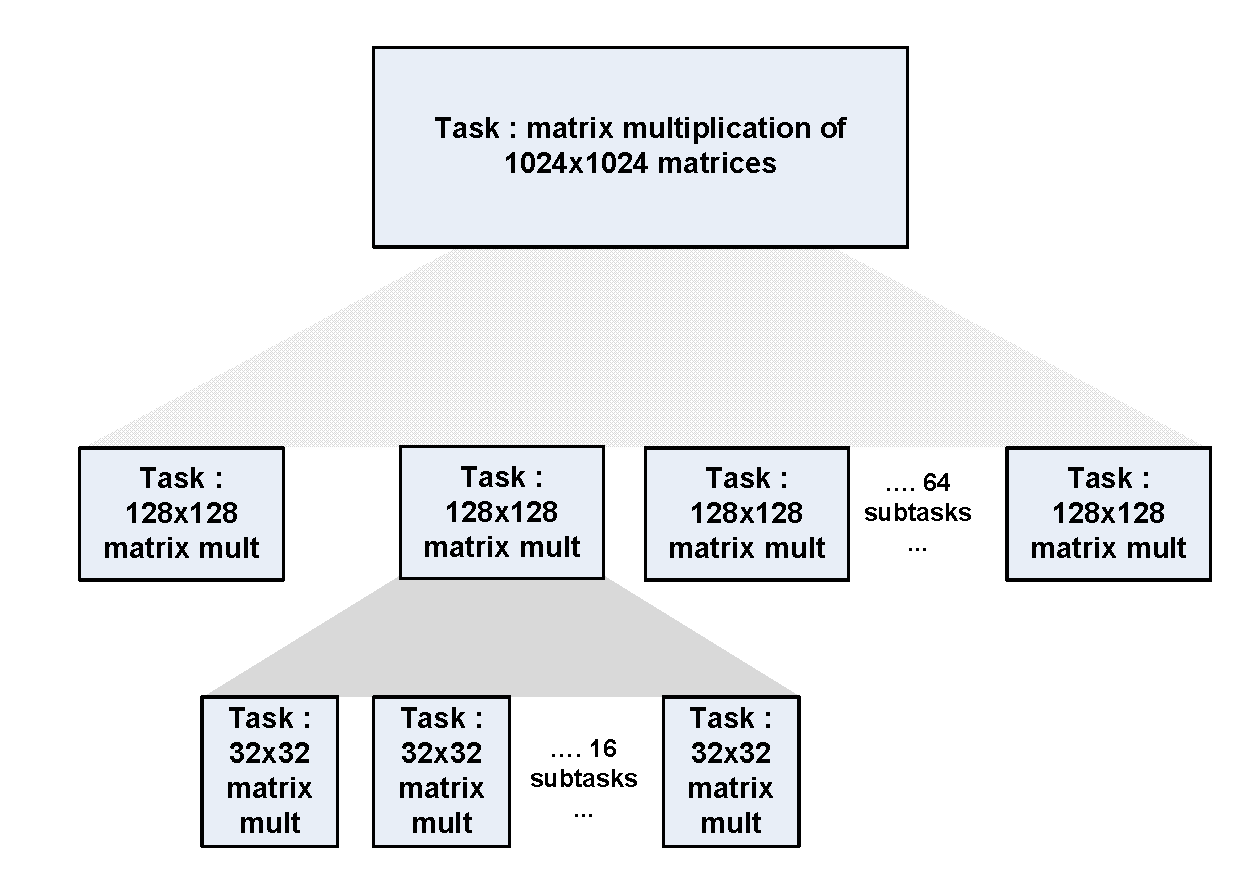
\includegraphics[scale =0.6]{Chapter1/figures/Sequoia_fig1}
	\caption{Multiplication de matrices de tailles 1024x1024 structur�e en hi�rarchie de t�ches ind�pendantes effectuant des multiplications sur des blocs de donn�es plus petits}
  \label{seq_fig1}
\end{figure}
Le principe de m�moire hi�rarchique est au coeur de l'outil \emph{\textbf{Sequoia}}, car dans les syst�mes modernes contenant plusieurs unit�s de traitement avec une hi�rarchie m�moire � plusieurs niveaux, il est primordial de diviser un calcul de taille importante en des op�rations plus petites pour atteindre des bonnes performances car cela permet d'exposer le parall�lisme et d'att�nuer l'effet de la latence d'acc�s � la m�moire car les donn�es sont physiquement proches des unit�s de traitement. Un exemple de d�coupage pour l'application produit de matrices est donn� dans \ref{seq_fig1}, dans cet exemple qui contient du parall�lisme imbriqu� et o� la localit� des donn�es est primordiale. \emph{\textbf{Sequoia}} requiert une telle r�organisation hi�rarchique dans les programmes, qui a �t� inspir�e de l'id�e des \emph{space-limited procedures} qui pr�ne les strategies \emph{divide-and-conquer} tenant compte de la hi�rarchie m�moire. Les \emph{space-limited procedures} requi�rent � chaque fonction dans une cha�ne d'appels d'accepter des arguments occupant beaucoup moins d'espace m�moire que les fonctions appellantes. Un syst�me complet a �t� impl�ment� autour de cette abstraction incluant un compilateur et un \textit{runtime} pour le processeur Cell.\\
L'�criture d'un programme \emph{\textbf{Sequoia}} implique la description abstraite d'une hi�rarchie de t�ches et le mapping de ces t�ches sur la hi�rarchie m�moire de la machine cible. Cela impose � l'utilisateur de considerer une machine parall�le comme un arbre de modules m�moire distincts. Les transferts de donn�es entre les niveaux de la hi�rarchie se font par blocks �ventuellement asynchrones. La logique du programme d�crit le transfert des donn�es � tous les niveaux, mais les noyaux de calcul sont contraints de travailles que sur les donn�es qui sont sur les noeuds feuilles (de niveau 0) de l'arbre repr�sentant la machine. La repr�sentation abstraite du processeur Cell (Fig.\ref{seq_fig2}) contient des noeuds correspondants � la m�moire principale ainsi qu'� chaque m�moire locale du SPE.
\begin{figure}[!htbf]
	\centering
	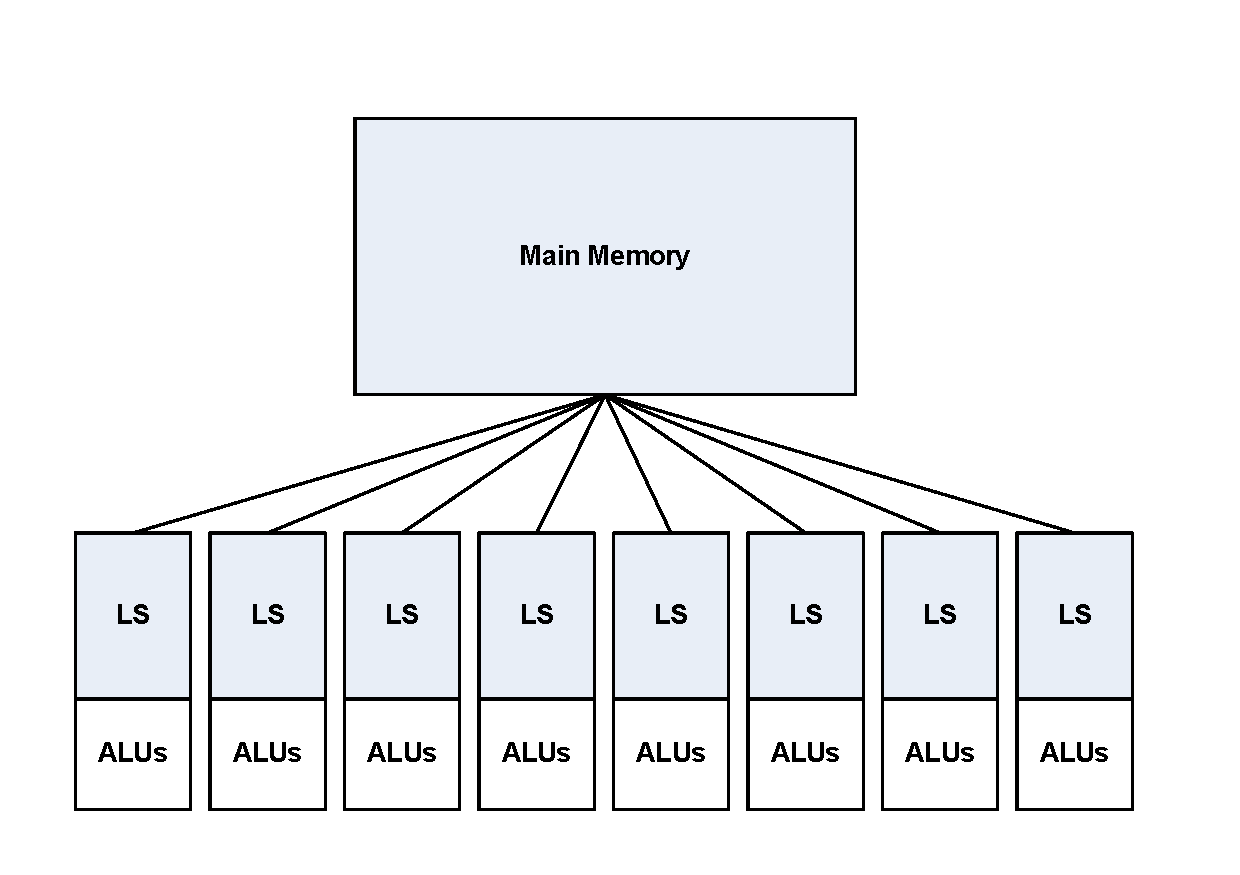
\includegraphics[scale =0.6]{Chapter1/figures/Sequoia_fig2}
	\caption{Mod�le abstrait Sequoia du processeur Cell}
  \label{seq_fig2}
\end{figure}
Un code \emph{\textbf{Sequoia}} ne fait pas de r�f�rence explicite � un certain niveau de la hi�rarchie et les transferts de donn�es entre les modules m�moire se font de mani�re implicite. Ainsi, les communications d�crites dans \emph{\textbf{Sequoia}} peut se faire au travers d'une instruction de prefetch, un transfert DMA ou un message MPI selon les sp�cificit� de l'architecture cible. Ceci garantit la portabilit� de l'application tout en b�n�ficiant des performances des communications explicites. Il y a certaines machines possedant une topologie qui n'est pas facilement representable sous forme d'arbre c'est pour cela que la notion de \emph{virtual level} (niveau virtuel) � �t� introduite dans \emph{\textbf{Sequoia}}, ce niveau ne correspond � aucune m�moire physique. Ce niveau permet par exemple de repr�senter l'aggregation des m�moires locales des SPEs sur processeur Cell. Cela permet de ce fait d'encapsuler les communications horizontales inter-noeud tout en gardant le mod�le d'abstraction en arbre qui lui ne permet que des communications verticales.
\subsection{Mod�le de Programmation}
La notion de \emph{task} est au coeur du mod�le de programmation de \emph{\textbf{Sequoia}}: c'est une fonction exempt de tout effet de bord avec une s�mantique de passage de param�tre par valeur. Les propri�t�s qui seront �nonc�es dans la suite garantissent la portabilit� du mod�le sans sacrifier les performances. Un exemple de code de multiplication de matrices par blocks est donn� dans le listing \ref{sequoiacode}.

\subsubsection{Communication Explicite et Localit�}
La d�finition d'une t�che exprime � la fois la localit� et la communication dans un programme. Lorsqu'une t�che s'ex�cute, l'ensemble de toutes les donn�es r�f�renc�es doivent rester dans un seul noeud de l'arbre abstrait de la machine. Ainsi une t�che doit s'ex�cuter dans un endroit pr�cis de la machine. Les pointeurs et les r�f�rences ne sont pas permises � l'int�rieur d'une t�che ce qui permet de dire que l'ensemble des donn�es trait�es par la t�che est contenu dans sa d�finition.\\
L'impl�mentation contient un appel r�cursif dans lequel un sous-ensemble des donn�es est pass� en param�tre. Les communications sont encapsul�es par les t�che en utilisant une s�mantique de passage de param�tre dit \emph{call-by-value-result} qui est un passage de param�tres par valeur dans lequel les copies locales des donn�es sont r��crites dans l'espace global � la fin de l'appel de la fonction. Chaque t�che s'ex�cute dans son espace d'adresses local, toutes les donn�es d'entr�e des t�ches appelantes sont copi�es dans l'espace m�moire de la fonction appel�e et les r�sultats sont recopi�es vers l'espace m�moire de la fonction appelantes apr�s le retour de la fonction appel�es.\\
Le mapping d'un programme Sequoia dicte quand une t�che appel�e doit ex�cut�e dans le m�me module m�moire que la t�che appelante ou alors assign�es � une m�moire enfant.

\subsubsection{Isolation et Parall�lisme}
La granularit� du parall�lisme dans \emph{\textbf{Sequoia}} et la \emph{t�che} et l'ex�cution parall�le r�sulte de l'appel de \emph{t�ches} concurrentes. Une t�che s'ex�cute g�n�ralement sur une partie de la boucle sous forme de plusieurs \emph{sous-t�ches} parall�les, chaque \emph{sous-t�che} s'ex�cutant en isolation, une propri�t� qui garantit la portabilit� et la performance. Une des contraintes impos�es au mod�les et que les t�ches s'ex�cutant en parall�le ne peuvent pas coop�rer entre elles car elles n'ont aucun moyen de communiquer. Ceci limite le mod�le de programmation au mod�le SPMD mais �vite le recours aux m�canismes de synchronisation co�teuses.
\subsubsection{D�composition de T�che}
\emph{\textbf{Sequoia}} introduit des primitives de d�composition de tableaux et de mapping de t�ches, elles sont d�crites ci-dessous:\\
\noindent \rule{\textwidth}{0.2mm}\\
\textbf{Sequoia Blocking Primitives}\\
\begin{itemize}
\item \texttt{\textbf{blkset}}\\
Un objet Sequoia opaque repr�sentant une collection de blocks de tableaux.\\
\item \texttt{\textbf{rchop(A, len0, len1, ...)}}\\
G�nere un \texttt{\textbf{blkset}} qui contient des blocks qui ne se recouvrent pas et qui tuilent le tableau multidimensionnel A. Chaque block est multidimensionnel de taille \texttt{len0xlen1x ...}.
\item \texttt{\textbf{rchop(A, rchop\_t(offset0, len0, stride0), ...)}}\\
G�n�ralisation de  \item \texttt{\textbf{rchop}} qui g�nere des ensembles de blocks qui contiennent potentiellement des blocks qui se recouvrent. L'offset du tableau de d�part, la taille du block, et le saut entre les blocks est sp�cifi� pour toutes ls dimensions du tableau source.
\item \texttt{\textbf{ichop(A, Starts, Ends, N)}}\\
G�n�re un ensemble de blocks du tableau A de tailles non r�guli�res. Les indices de d�part et de fin du block sont donn�s par les �l�ments dans le tableau de longueur N \texttt{Starts} et \texttt{Ends}. 
\item \texttt{\textbf{gather(A, IdxBlkset)}}\\
G�n�re un ensemble de blocks en rassemblant les �l�ments d'un tableau source A en utilisant des indices fournis dans les blocks de \texttt{IdxBlkset}. Le \texttt{blkset } r�sultant poss�de les m�mes nombre et taille que les blocks de \texttt{IdxBlkset}.\\
\end{itemize}
\rule{\textwidth}{0.2mm}\\
\textbf{Sequoia Mapping Primitives}\\
\begin{itemize}
\item \texttt{\textbf{mappar(i=i0 to iM, j=j0 to jN ...)   {...}}}\\
Une boule for multi-dimensionnelle contenant uniquement un appel � une \emph{sous-t�che} dans le corps de boucle. La t�che est mapp�e en parall�le en une collection de blocks.
\item \texttt{\textbf{mapseq(i=i0 to iM, j=j0 to jN ...)   {...}}}\\
Une boule multi-dimensionnelle contenant uniquement un appel � une \emph{sous-t�che} dans le corps de boucle. La t�che est mapp�e s�quentiellement en une collection de blocks.
\item \texttt{\textbf{mapreduce(i=i0 to iM, j=j0 to jN ...)   {...}}}\\
Permet de faire le mapping en une collection de blocks, qui effectue une r�duction sur au moins un argument de la t�che. Pour le support des r�ductions d'arbres parall�les, une t�che suppl�mentaires de
 recombinaison est requise.\\
\end{itemize}
\rule{\textwidth}{0.2mm}\\
\subsubsection{Variantes de T�ches}
\emph{\textbf{Sequoia}} inclut deux types de t�ches qui servent essentiellement � distinguer le code de mapping du code de calcul, elles sont d�crites ci-dessous:
\begin{itemize}
\item \emph{Inner Tasks}: se sont les t�ches qui appellent des sous-t�ches. Elles n'ont pas d'acc�s direct � leurs arguments de type tableau mais elles passent aux sous-t�ches sous forme de blocks. Les \emph{Inner Tasks} utilisent les primitives de \emph{mapping} et de \emph{blocking} pour structurer les calculs sous forme de sous-t�ches. La d�finition d'une \emph{Inner Task} n'est associ�e � aucun module m�moire particulier de la machine, elle peu s'ex�cuter dans n'importe quel niveau de la hi�rarchie m�moire dans lequel les donn�es trait�es tiennent.
\item \emph{Leaf Tasks}: se sont des t�ches qui ne font pas appel � des sous-t�ches et qui op�rent directement sur des donn�es r�sident dans les niveaux feuilles de la hi�rarchie m�moire. 
\end{itemize}

\subsubsection{Param�trisation de T�ches}
Les t�ches sont �crite de mani�re � ce qu'elles soient param�trables pour la sp�cialisation � de multiples machines cibles. La sp�cialisation est le processus de de cr�ation d'instances d'une t�che qui est personnalis� pour s'ex�cuter sur un certain niveau de la hi�rarchie m�moire de la machine. La param�trisation des t�ches permet � une strat�gie de d�composition d�crite par une variante de t�che d'�tre appliqu�e dans diff�rents contextes, rendant la t�che portable sur diff�rentes machines et sur diff�rentes niveaux de la hi�rarchie m�moire d'une cible donn�e. L'utilisation de param�tres comme la taille des tableaux ainsi que les param�tres ajustable decouple l'expression d'un algorithme de son impl�mentation sur une machine donn�e.
\subsubsection{Sp�cialisation de T�ches et Tunning}
Dans \emph{\textbf{Sequoia}} on donne au programmeur le contr�le complet sur les phases de sp�cialisation et de tunning du code, au travers d'une phase dite de \emph{task mapping and specification} qui est cr��e par l'utilisateur pour une machine donn�e est maintenue ind�pendamment du code source. En plus, cette phase permet au programmeur de fournir des directives d'optimisation et de tunning qui sont propres � une cible donn�e. 
Les sp�cification de mapping ont pour but de donner � l'utilisateur un contr�le pr�cis sur le mapping d'une hi�rarchie de  t�ches sur une machine en isolant les optimisations sp�cifiques � une cible donn�e dans un autre endroit. Au lieu de confier le travail � un compilateur, \emph{\textbf{Sequoia}} permet au programmeur d'optimiser son code lui m�me afin d'obtenir les meilleurs performances possibles.
%===============================Listing Sequoia=======================================
\lstset{ %
language=C,                % choose the language of the code
basicstyle=\footnotesize,       % the size of the fonts that are used for the code
backgroundcolor=\color{light-gray},  % choose the background color. You must add \usepackage{color}
showspaces=false,               % show spaces adding particular underscores
showstringspaces=false,         % underline spaces within strings
showtabs=false,                 % show tabs within strings adding particular underscores
frame=single,			% adds a frame around the code
tabsize=2,			% sets default tabsize to 2 spaces
captionpos=b,			% sets the caption-position to bottom
breaklines=true,		% sets automatic line breaking
breakatwhitespace=false,	% sets if automatic breaks should only happen at whitespace
escapeinside={\%*}{*)}  ,        % if you want to add a comment within your code
caption = Exemple de multiplication matricielle par blocks \emph{Sequoia} ,
label = sequoiacode
}
\lstinputlisting{Chapter1/Code/sequoia.c}
%===================================================================================
\subsection{Impl�mentation}
Dans l'impl�mentation de \emph{\textbf{Sequoia}} un compilateur source-to-source g�n�re du code C qui s'interface avec un \textit{runtime} sp�cifique � la plate-forme. Les param�tres d'entr�e du compilateur sont un program \emph{\textbf{Sequoia}} ainsi que des sp�cifications de mapping sur la machine cible.
\subsubsection{Compilateur Cell et \textit{runtime}}
Les instances de t�ches \emph{Inner} correspondant � la m�moire principale sont ex�cut�es par le PPE alors que les instances correspondant au niveau m�moire des Local Store sont ex�cut�es par les SPE. Les codes sources PPE et SPE sont compil�s s�paremment, un code binaire est ainsi combin� pour l'ex�cution, si toutefois le code SPE d�passe la capacit� du local store il est d�coup� sous forme d'overlays. Le \textit{runtime} est \emph{event driven}: un syst�me de notification via mailbox est mis en place entre le PPE est les SPES, les t�ches sont assign�e par le PPE au SPE. Une fois que la notification est re�ue un m�canisme du \textit{runtime} charge le morceau de code � ex�cuter dans les SPEs et initie les transfers de donn�es via DMA. Le syst�me permet la superposition de transferts et de calculs afin d'am�liorer les performances. Les m�canismes de synchronisation ne sont pas constamment utilis�es entre les t�ches, un seul point de synchronisation est requis lors de la fin des sections parall�les,ce qui minimise  l'overhead.
\subsubsection{Optimisations}
En plus de permettre au programmeur d'optimiser son impl�mentation des t�ches dans \emph{\textbf{Sequoia}}, certaines optimisations qui � utiliser efficacement la m�moire sont utilis�es, notamment l'optimisation des transferts au niveau d'un m�me niveau la hi�rarchie m�moire, ou les copies inutiles sont d�tect�es et supprim�es. D'autres optimisation incluant le \emph{software-pipelining} et le d�placement des invariants de boucle sont effectu�s de mani�re statique � la compilation.
\subsection{Conclusion}
\emph{\textbf{Sequoia}} est un mod�le de programmation qui tente d'allier la portabilit� avec la performance pour le portage d'algorithmes sur des architectures parall�les. La performance est assur�e par l'octroi � l'utilisateur d'une grande libert� dans l'optimisation du code de calcul qui s'ex�cute sur les noeuds au plus bas niveau de la hi�rarchie m�moire. La portabilit� est garantie par le fait que l'expression de l'algorithme est d�coupl�e de l'impl�mentation. L'expression explicite des communications, du mouvement des donn�es au travers de la hi�rarchie m�moire, du calcul parall�le et la d�finition d'un ensemble de travail isol� sont effectu�s gr�ce � une seule abstraction, la \emph{t�che}. \emph{\textbf{Sequoia}} fournit des primitives de structuration des calcul en tant que hi�rarchie de t�ches afin d'am�liorer la localit� et laisse au programmeur le soin d'optimiser la t�che pour une architecture donn�e. Toutefois il existe des limitations, en l'occurrence pour le type de parall�lisme qui doit �tre SIMD ce qui limite le sch�ma de d�ploiement et le champ d'applications. Aussi, le mapping des applications est fait de mani�re manuelle et n'est pas contenue dans le code source.

\section{Squelettes Algorithmiques pour le Cell}
La programmation parall�le structur�e qu'on appelle programmation par squelettes algorithmiques \cite{skeletons_cole} restraint l'expression du parall�lisme � la composition d'un nombre pr�d�fini de \emph{patterns} nomm�s squelettes. Les squelettes algorithmiques sont des briques de base g�n�riques, portables et r�utilisables pour lesquelles une impl�mentation parall�le peut exister. Ils sont issues des langages de programmation fonctionnelle. Un syst�me de programmation bas� sur les squelettes fournit un ensemble fixe et relativement limit� de squelettes. Chaque squelette repr�sente une mani�re unique d'exploiter le parall�lisme dans une organisation sp�cifique du calcul, tels que le parall�lisme de donn�es, de t�ches, le \emph{divide-and-conquer} parall�le ou encore le pipeline. En combinant ces \emph{patterns} le d�veloppeur peut construire une sp�cification haut-niveau de son programme parall�le. Le syst�me peut ainsi exploiter cette sp�cification pour la transformation de code, l'exploitant efficace des ressources ou encore le placement.\\
La composition des squelettes peut se faire d'une mani�re non-hi�rarchique en mettant en s�quence les diff�rents blocs en en utilisant des variables temporaires pour sauvegarder les r�sultats interm�diaires, ou alors de mani�re hi�rarchique en imbriquant les fonctions squelette et ce en construisant une fonction compos�e dans laquelle le code de plusieurs squelettes est pass� en param�tre d'un autre squelette. Ceci pr�sente une mani�re �l�gante d'exprimer le parall�lisme multi-niveau.\\
Dans un environnement de programmation declarative, comme dans les langages fonctionnels ou alors dans la programmation par squelettes, la composition hi�rarchique procure au g�n�rateur de code plus de libert� de choix pour les transformations automatiques et l'utilisation efficace des ressources, comme par exemple le nombre de processeurs utilis� en parall�le dans un niveau particulier de la hi�rarchie. les squelettes ne pouvant pas �tre imbriqu�s  sont g�n�ralement impl�ment�es avec juste une librairie g�n�rique alors que les squelettes nich�s requi�rent un pr�-traitement qui d�roule la hi�rarchie du squelette en utilisant par exemple les templates C++ ou les macros de preprocesseur en C.
%pardo,pipe,seq et chain
\subsection{Mod�le de Programmation}
\begin{figure}[!htb]
	\centering
  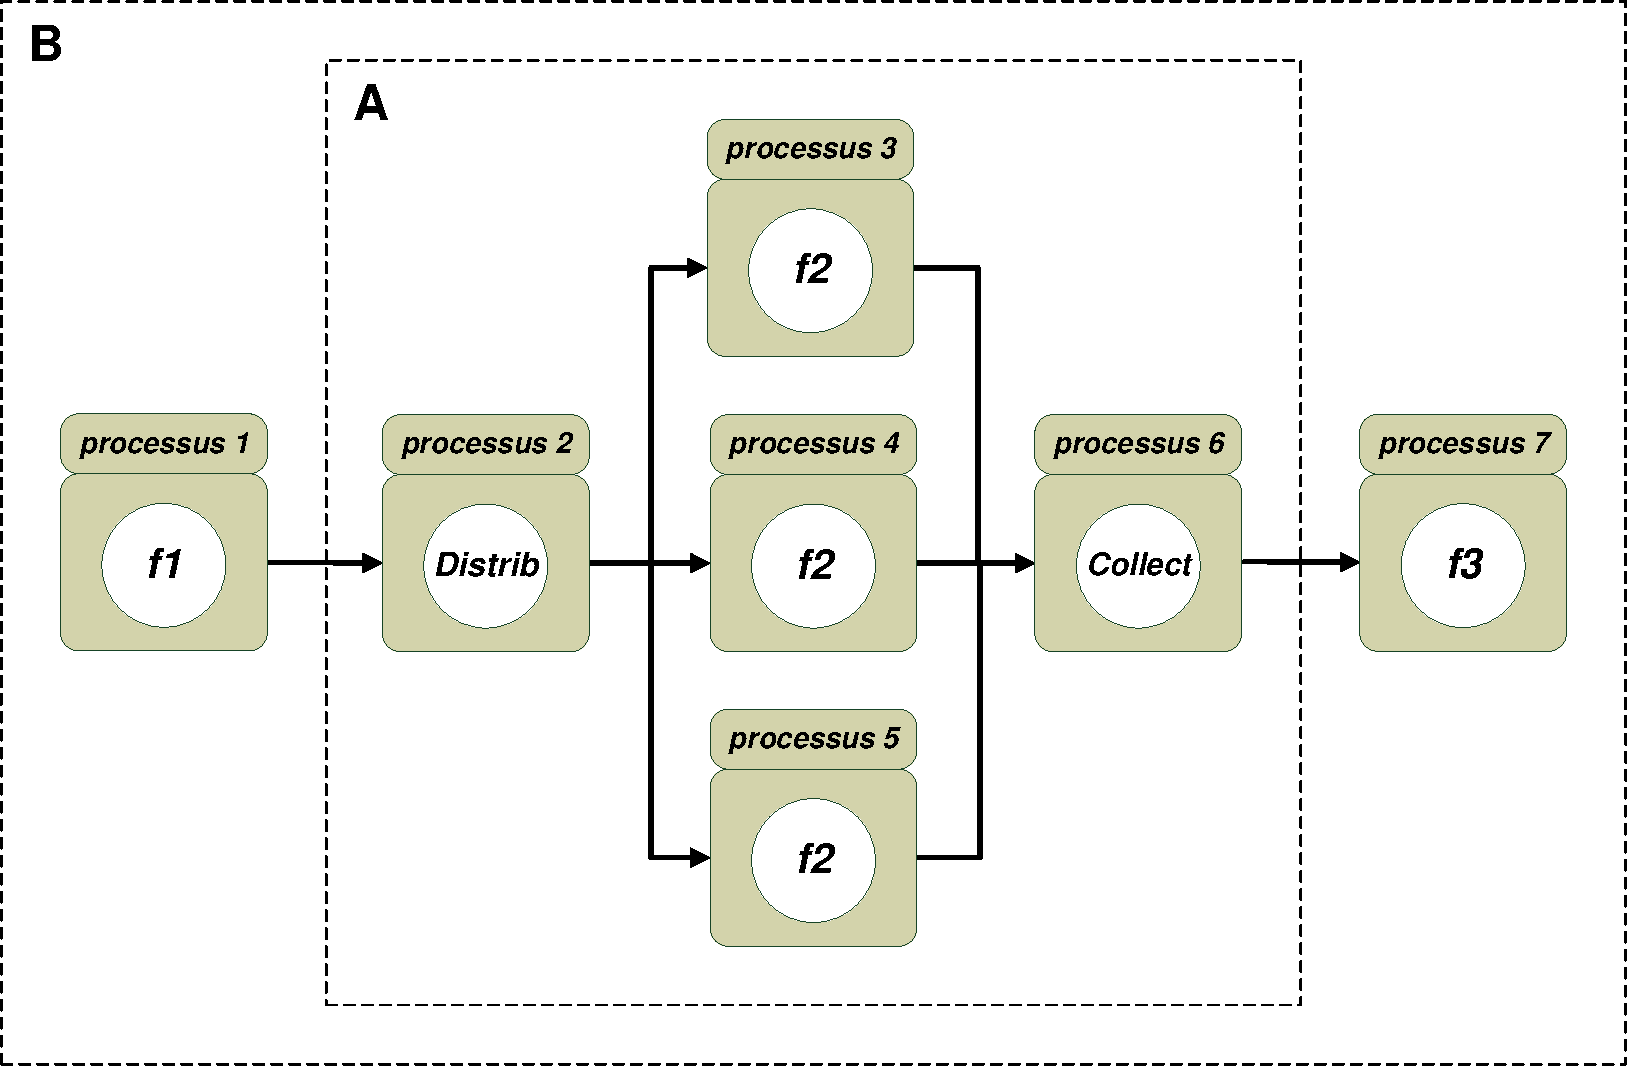
\includegraphics[width= 0.8\columnwidth]{Chapter1/figures/skeleton_example}
	\caption{Exemple de graphe de processus communicants avec hi�rarchisation}
	\label{skelexple}
\end{figure}
Dans le mod�le de programmation parall�le par squelettes algorithmiques, une application est d�finie comme �tant un graphe de processus communicants. Cette repr�sentation permet de sp�cifier les sch�mas de communication entre les processus \textbf{$P_{i}$}, de mettre en �vidence les fonctions s�quentielles \textbf{$F_{i}$} contenues dans l'application, ainsi que les processus n�cessaires � l'ex�cution parall�le de l'application. Un exemple de repr�sentation est donn� dans la figure \ref{skelexple}. On peut distinguer sur cette figure deux parties distinctes : 
\begin{itemize}
\item Le syst�me d'�quilibrage de charge \textbf{(A)} qui utilise $k$ processeurs qui traite les donn�es fournies par le processus \emph{Distrib}, ces derni�res �tant regroup�es par le processus \emph{Collect}. Il faudra noter que le flux alimente le processeurs de mani�re dynamique d�s qu'il trouve un processus libre.
\item Le m�canisme de contr�le \textbf{(A)} qui permet de s�quencer les traitement dans l'ordre donn�e par le graphe. Ce m�canisme assure que les donn�es, une fois trait�es (fonction $F_{i}$) par le processeur $P_{i}$, sont transmises au processus $P_{i+1}$. On pourra noter que le sch�ma d'ex�cution dans ce cas l� est du type \emph{pipeline}.
\end{itemize}
Le mod�le de programmation parall�le par squelettes algorithmiques repose sur l'extraction de tels sch�mas r�currents. Un squelette est ainsi d�fini comme �tant un sch�ma g�n�rique param�tr� par une liste de fonctions qu'il est possible d'instancier et de composer. Fonctionnellement, les squelettes algorithmiques sont des \textbf{fonctions d'ordre sup�rieur}, c'est � dire des fonctions prenant une ou plusieurs fonctions comme arguments et retournant une fonction comme r�sultat. La programmation par squelettes devient permet au programmeur d'utiliser un mod�le haut-niveau pour d�crire son application, sans se soucier de certains d�tails complexes comme l'ordonnancement ou le placement. Il peut alors d�finir une application parall�le comme suit:
\begin{itemize}
\item Instancier des squelettes en sp�cifiant les fonctions qui les d�finissent.
\item Exprimer la composition des ces squelettes.
\end{itemize}
L�expression de la compositions peut se faire en encodant cette derni�re sous la forme d�un \textbf{arbre}(\ref{fig_tree}) dont les noeuds repr�sentent les squelettes utilis�s et les feuilles, les fonctions s�quentielles pass�es en param�tres � ces squelettes.
\begin{figure}[!htb]
	\centering
  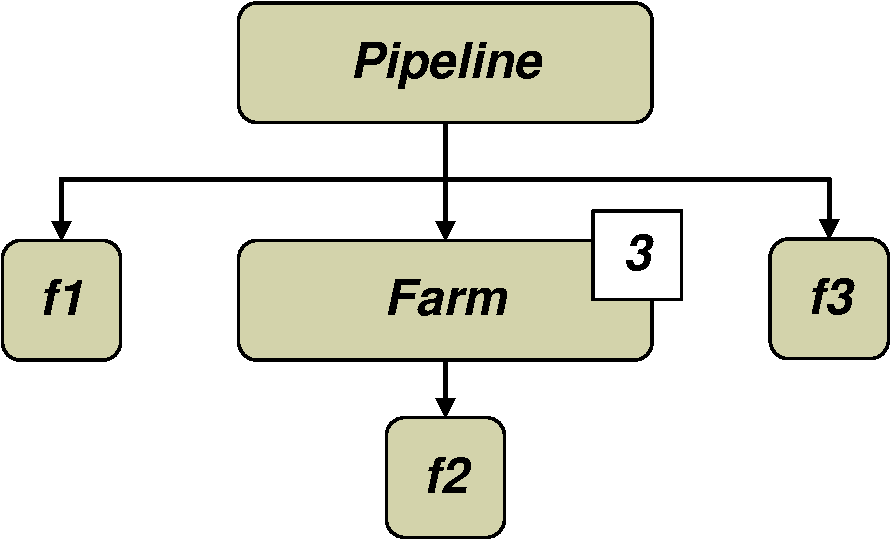
\includegraphics[width= 0.7\columnwidth]{Chapter1/figures/fig_tree}
	\caption{Arbre repr�sentant le squelette en Figure \ref{skelexple}}
	\label{fig_tree}
\end{figure}
Dans la figure \ref{fig_tree}, le squelette \textbf{Pipeline} d�crit le sch�ma g�n�rique correspondant � la section \textbf{B} du graphe de processus communiquant initial. Le squelette \textbf{Farm} repr�sente quant � lui la partie \textbf{A} de ce m�me sch�ma. Les fonctions $F_{i}$ apparaissent aux feuilles de l'arbre, c'est � dire en argument des squelettes. On note aussi que les fonctions \textbf{Distrib} et Collect n'apparaissent plus explicitement, car elles font partie int�grante du squelette \textbf{Farm}. Cette repr�sentation met en avant un des aspects les plus importants de l'approche
� base de squelettes algorithmiques : � partir d'un nombre restreint de squelettes (classiquement moins d'une dizaine), il est possible de d�finir des applications complexes. Ceci suppose toutefois que l'on ait formalis� le type d'application que l'on va chercher � parall�liser, de d�finir pr�cis�ment le jeu de squelettes que l'on d�sire mettre � disposition du d�veloppeur et de sp�cifier leurs s�mantiques fonctionnelles et op�rationnelles. Il existe plusieurs classifications des squelettes. Toutefois, on peut les r�partir en trois groupes : les squelettes d�di�s au parall�lisme de contr�le, les squelettes d�di�s au parall�lisme de donn�es et les squelettes d�di�s � la structuration s�quentielle de l�application.
\subsubsection{Squelettes d�di�s au parall�lisme de contr�le}
%pardo,pipe,seq et chain
\paragraph{Le Squelette Pipeline}
Ce squelette couvre les situations dans laquelle une liste de fonction qui doivent s'ex�cuter en s�rie, est r�partie sur un ensemble de processeurs diff�rents. En r�gime permanent l'ex�cution de la fonction $F_{i}$ sur les donn�es $D_{i+1}$ se fait alors en parall�le avec celle de la fonction $F_{i+1}$ sur les donn�es $D_{i}$. La figure \ref{skell-pipe} illustre ce fonctionnement en r�gime permanent.
\begin{figure}[!htb]
	\centering
  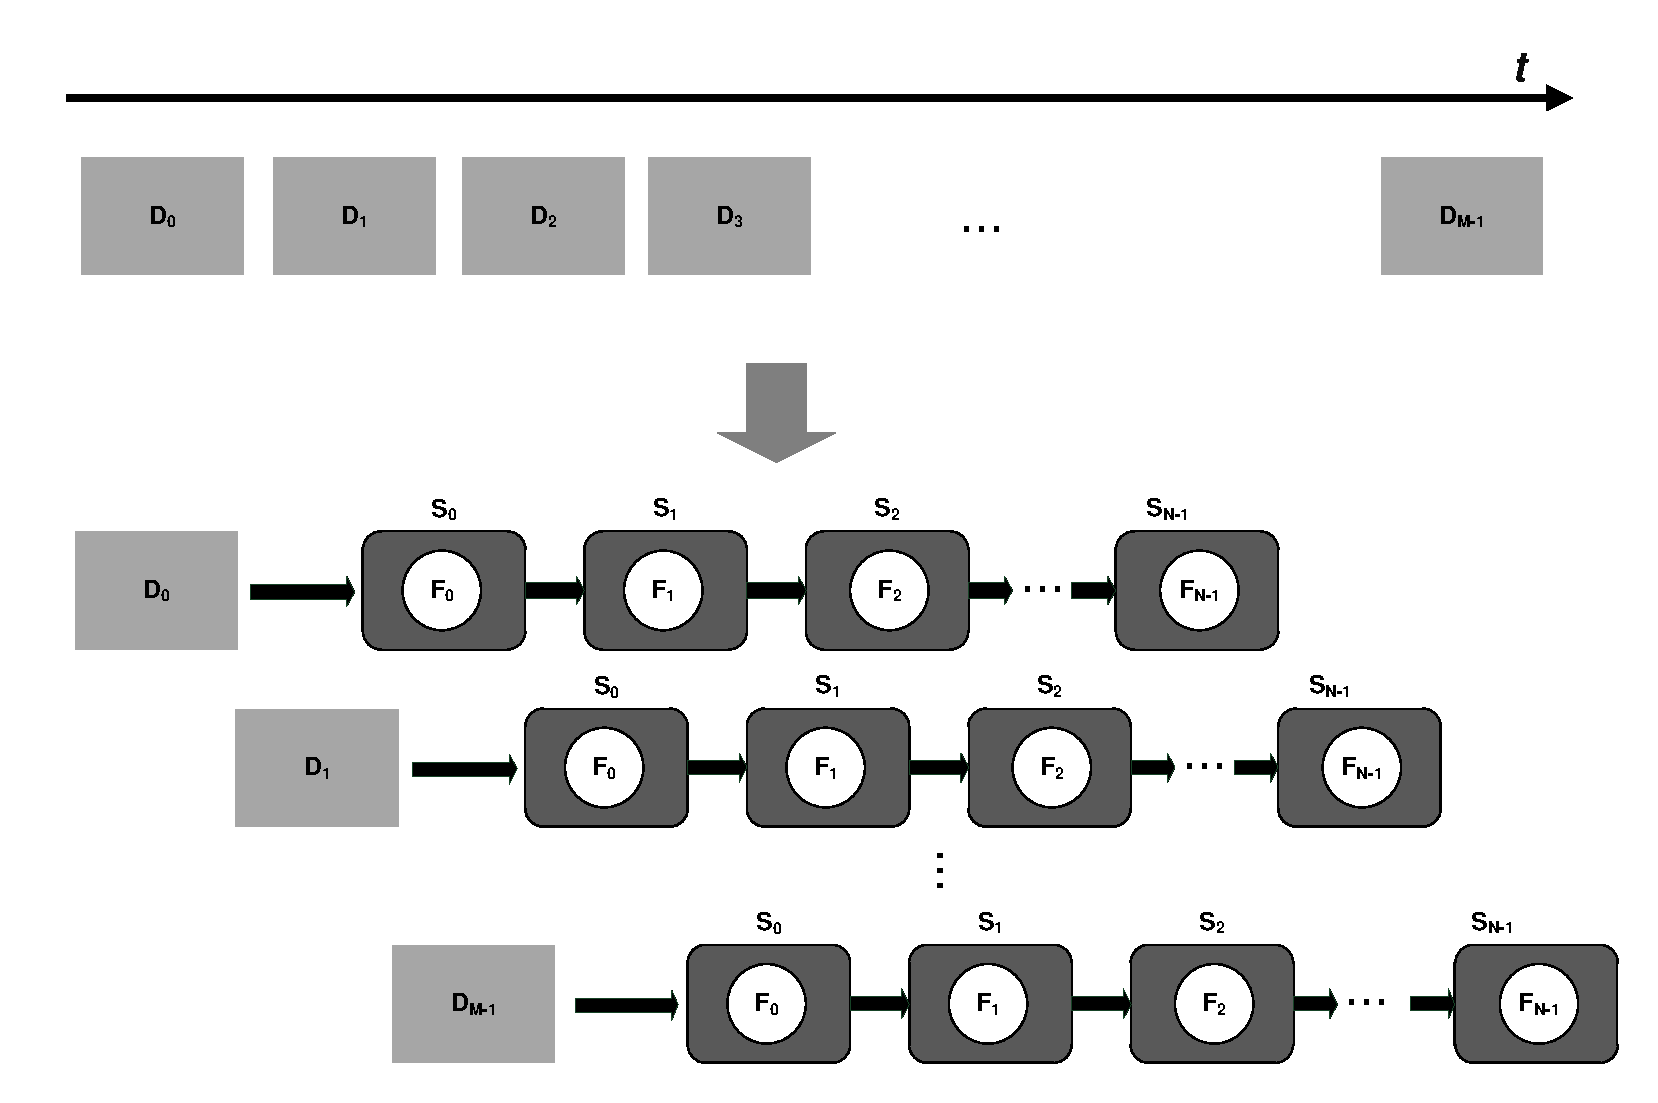
\includegraphics[width= \columnwidth]{Chapter1/figures/skell-pipe}
	\caption{Exemple de squelette du type \textbf{Pipeline}}
	\label{skell-pipe}
\end{figure}
Le parall�lisme r�sulte du fait que l'�valuation des diff�rents fonctions du \textbf{Pipeline} sur des �l�ments diff�rents du flux ($D_{0}$, $D_{1}$ par exemple sur la figure \ref{skell-pipe}) se fait de mani�re ind�pendante. Deux grandeurs caract�risent alors le \textbf{Pipeline} : (1)la latence qui est la dur�e de traitement d'un �l�ment de flux par tous les �tages du pipeline, (2) le d�bit, qui mesure le nombre de r�sultats fournis par unit�s de temps et qui est d�termin� par l'�tage le plus lent du \textbf{Pipeline}.
\paragraph{Le Squelette Pardo}
\begin{figure}[!htb]
	\centering
  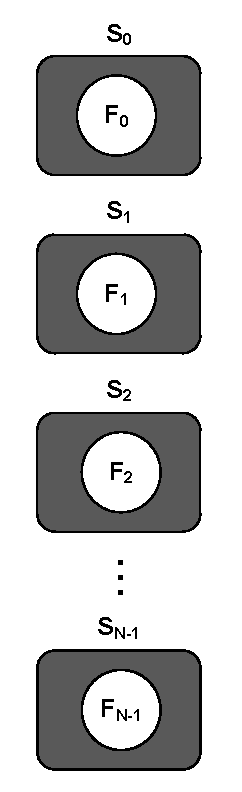
\includegraphics[width= 0.2\columnwidth]{Chapter1/figures/skell-pardo}
	\caption{Exemple de squelette du type \textbf{Pardo}}
	\label{skell-pardo}
\end{figure}
Le squelette \textbf{Pardo} permet de placer de mani�re \emph{ad hoc} $N$  fonctions sur $N$ processeurs (Fig. \ref{skell-pardo}). Le sch�ma de communication est alors implicite. Ce type de squelette est fait pour faciliter la mise en oeuvre d'applications qui ne correspondent pas � un squelette bien d�fini. Le squelette \textbf{Pardo} est notamment utilis� pour rassembler plusieurs fonctions ind�pendantes op�rant sur un flux de donn�es. Le temps d'ex�cution d'un tel sch�ma est alors celui de la fonction qui prend le plus de temps � s'ex�cuter. 
\subsection{Squelettes d�di�s � la structuration de l�application}
\subsubsection{Le Squelette Sequence}
\subsubsection{Le Squelette Select}
\subsection{Mod�le de Programmation \texttt{SKELL\_BE}}
Dans le mod�le de programmation \texttt{SKELL\_BE} \cite{skellbepact}, le processeur Cell est consid�r� comme une machine asym�trique. Le mod�le inclue deux codes source, un pour le PPE et un autre pour le SPE. Du point de vue du PPE une application peut appeler un \emph{kernel} de calcul qui est compil� et ex�cut� sur le SPE comme dans une application de \emph{stream processing} (\ref{skellbe01}.
%===============================Listing PPEKERNEL =======================================
\lstset{ %
language=C,                % choose the language of the code
basicstyle=\footnotesize,       % the size of the fonts that are used for the code
backgroundcolor=\color{light-gray},  % choose the background color. You must add \usepackage{color}
showspaces=false,               % show spaces adding particular underscores
showstringspaces=false,         % underline spaces within strings
showtabs=false,                 % show tabs within strings adding particular underscores
frame=single,			% adds a frame around the code
tabsize=2,			% sets default tabsize to 2 spaces
numbers=left,                   % where to put the line-numbers
captionpos=b,			% sets the caption-position to bottom
breaklines=true,		% sets automatic line breaking
breakatwhitespace=false,	% sets if automatic breaks should only happen at whitespace
escapeinside={\%*}{*)}  ,        % if you want to add a comment within your code
caption = Exemple d'un appel � un kernel PPE dans \texttt{SKELL\_BE},
label = skellbe01
}
\lstinputlisting{Chapter1/Code/ppekernel.c}
%===================================================================================
Un \emph{kernel} est d�fini par la macro \texttt{SKELL\_KERNEL} comme un prototype de fonction dans lequel les arguments pass�s par r�f�rence sont consid�r�s comme des sorties du \emph{kernel}, alors que les arguments pass�es par valeur ou par r�f�rence contante sont les entr�es su \emph{kernel}. La ligne 9 du listing \ref{skellbe01} montre un exemple d'appel de \emph{kernel} au \emph{runtime}, l'initialisation du processeur Cell qui est effectu�e par un appel � \texttt{skell:environment} d�marre un groupe de \emph{threads} SPE et les mets en attente d'un appel � un \emph{kernel} ce qui r�duit le surco�t de cr�ation de \emph{threads} � chaque fois. La terminaison des \emph{threads} est effectu�e de la m�me mani�re � la fin de la port�e de la fonction \emph{main}.\\
\indent Du point de vue des SPEs, chacun d'eux est un neoud de \emph{cluster} qui supporte la communication point-�-point. Les applications sont con�us � base d'une  composition de squelettes instanci�es avec des fonctions d�finies par l'utilisateur qui consid�rent la m�moire centrale comme un m�moire distante � partir de laquelle peuvent �tre lues ou �crite de mani�re asynchrone au travers des commandes DMA de la librairie standard ou � des fonctions fournies par \texttt{SKELl\_BE} \ref{skellbe02}.

%===============================Listing SPEKERNEL =======================================
\lstset{ %
language=C,                % choose the language of the code
basicstyle=\footnotesize,       % the size of the fonts that are used for the code
backgroundcolor=\color{light-gray},  % choose the background color. You must add \usepackage{color}
showspaces=false,               % show spaces adding particular underscores
showstringspaces=false,         % underline spaces within strings
showtabs=false,                 % show tabs within strings adding particular underscores
frame=single,			% adds a frame around the code
tabsize=2,			% sets default tabsize to 2 spaces
numbers=left,                   % where to put the line-numbers
captionpos=b,			% sets the caption-position to bottom
breaklines=true,		% sets automatic line breaking
breakatwhitespace=false,	% sets if automatic breaks should only happen at whitespace
escapeinside={\%*}{*)}  ,        % if you want to add a comment within your code
caption = Exemple de d�finition d'un kernel SPE dans \texttt{SKELL\_BE},
label = skellbe02
}
\lstinputlisting{Chapter1/Code/spekernel.c}
%======================Conclusion G�n�rale ==================================
Ce dernier code source illustre plusieurs aspects :
\begin{itemize}
\item la macro \texttt{SKELL\_BE} g�n�re le \emph{stub} de la fonction \texttt{main} et l'introspection de code requise par \texttt{SKELL\_BE}.
\item la fonction \texttt{run} qui est utilis�e dans la foncion de \emph{kernel} pour construire une aplication en utilisant les constructeurs de squelettes \texttt{pardo} et \texttt{seq}.
\item l'objet \texttt{argN\_} qui fournit un acc�s transparent au $N^{i�me}$ argument du \emph{kernel} stock� dans la m�moire centrale.
\item les fonction \texttt{pull} et \texttt{push} qui permettent un acc�s asynchrone � la m�moire principale adress�e par le PPE. Ces fonctions d�duisent la meilleurs mani�re de rapatrier les donn�es � partir de leurs arguments et utilisent un d�coupage statique des donn�es � partir du nombre de SPEs impliqu�es et de la taille de leur m�moire priv�e. 
\item La fonction \texttt{terminate} d�clenche la terminaison du \emph{kernel}. Celle-ci n'est appel�e qu'une fois per \emph{kernel}, d�s que toutes les donn�es transf�r�es de la m�moire centrale on �t� trait�es.
\end{itemize}
Le tableau \ref{skellbeapi} r�sume les principales fonctions de l'interface utilisateur (API) de \texttt{SKELL\_BE}.
\begin{table}
\centering
%\begin{tabular}{ll}
\begin{tabularx}{\columnwidth}{lX}
\hline
\hline
\textbf{Gestion de l'Application} & \\
\hline
\hline
\texttt{environement(argc,argv)} & D�marrage de l'application\\
\hline
\texttt{rank()}      & retourne l'indentifiant PID su SPE courant \\
\hline
\texttt{terminate()} & Signale la fin du flux de donn�es et termine l'application\\
\hline
\texttt{run(skeleton)}      & Execute une application squelette\\
\hline
\hline
\textbf{Constructeurs de Squelettes}& \\
\hline
\hline
\texttt{seq(f)} & Transforme une fonction utilisateur en une t�che squelette\\
\hline
\texttt{operator,(s$_1$,s$_2$)}       & \\
\texttt{chain(s$_1$,$\ldots$,s$_n$)}  & Constructeur de composition s�quentielle\\
\texttt{chain<N>(s)}                  & \\
\hline
\texttt{operator|(s$_1$,s$_2$)}          & \\
\texttt{pipeline(s$_1$,$\ldots$,s$_n$)}  & Constructeur de \emph{Pipeline}\\
\texttt{pipeline<N>(s)}                  & \\
\hline
\texttt{operator\&(s$_1$,s$_2$)}       & \\
\texttt{pardo(s$_1$,$\ldots$,s$_n$)}  & Constructeur de \emph{Pardo}\\
\texttt{pardo<N>(s)}   		      & \\
\hline
\hline
\textbf{Transfert de Donn�es} & \\
\hline
\hline
\texttt{pull(arg$_N$,v,sz=0,o=0)}   & R�cup�re $sz$ �l�ments de la  $N^{i�me}$ donn�e de la m�moire centrale
                                      et les sauvegarde dans $v$ avec un \emph{offset} $o$\\
\hline
\texttt{push(arg$_N$,v,sz=0,o=0))}  & Envoie $sz$ �l�ments de la donn�e $v$ � la  $N^{i�me}$ donn�e dans la m�moire
                                      centrale avec un \emph{offset} $o$\\
\hline
\hline
%\end{tabular}
\end{tabularx}
\caption{Interface utilisateur \texttt{SKELL\_BE}}
\label{skellbeapi}
\end{table}

\subsection{D�tails de l'Impl�mentation}
Le d�veloppement d'une librairie de calcul parall�le � base squelettes algorithmiques � la fois efficace et expressive est une t�che complexe. Plusieurs tentavies ont montr� que le compromis entre expressivit� et efficacit� �tait d�terminant pour le succ�s d'une telle librairie. Le polymorphisme est � premi�re vue une bonne solution pour exprimer la relation entre les squelettes et les objets fonctions, l'exp�rience d�montre que l'\emph{overhead} induit par son \emph{runtime} affecte consid�rablement la performance globale d'une application. Dans le cas des squelette le polymorphisme au runtime n'est pas vraiment n�cessaire : par conception, la structure d'une application exprim�e sous forme de squelettes imbriqu�s est connue � la compilation. Il suffit juste de trouver une mani�re propre d'exploiter cette information disponible � la compilation d'une mani�re judicieuse.\\
\indent Consid�rons les constructeurs de squelettes comme des mots-cl�s d'un petit langage d�claratif \emph{domain-specific}\footnote{en opposition � un langage \emph{general-purpose}}. L'information sur l'application � g�n�rer est donn�e par la s�mantique op�rationnelle de ces constructeurs. Dans notre cas, le d�fi �tait de trouver une mani�re de d�finir un tel langage comme une extension de C++ qui d�finit un EDSL (\emph{Embedded Domain Specific Language}), sans construire une nouvelle variation d'un compilateur mais seulement en utilisant la m�ta-programmation.\\
La m�ta-programmation est un ensemble de techniques h�rit�es de la programmation g�n�rative qui permet la manipulation, la g�n�ration et l'introspection de fragments de code dans un langage. A titre comparatif, lorsqu'une fonction est ex�cut�e au \emph{runtime} pour produire des valeurs � l'ex�cution, une m�ta-fonction op�re � la compilation sur des fragments de code pour g�n�rer des fragments de code plus sp�cialis�s qui seront compil�s. l'ex�cution d'un tel code se fait par cons�quent en deux passes. En C++, un tel syst�me est mis en oeuvre par les classes et les fonctions \emph{template}. En utilisant la flexibilit� de la surcharge d'op�rateur et de fonctions en C++ et le fait que les \emph{templates} C++ peuvent effectuer des calculs arbitraires � la compilation, on peut �valuer la structure d'une application parall�le d�crite par une combinaison de squelettes \textbf{� la compilation}. Pour ce faire, la structure extraite de la d�finition de l'application doit �tre transform�e en une repr�sentation interm�diaire bas�e sur un r�seau de \emph{processes} s�quentiels. Dans le cas de \texttt{SKELL\_BE} la difficult� fut d'enfouir les constructeur de squelettes dans des �l�ments de langage, de g�n�rer le code sur les SPEs et d'effectuer le transfert d'arguments entre le PPE et les SPEs.
\subsection{G�n�ration de Code pour les SPEs}
L'impl�mentation d'un \emph{EDSL} en C++ impose d'avoir une m�thode pour trouver de mani�re ad�quate des informations non-triviales � partir de l'arbre de syntaxe abstraite d'une expression (\emph{AST}). Ceci est effectu� en g�n�ral � l'aide d'une technique connue sous le nom de \emph{Expression Templates} \cite{exp_tpl}. Les \emph{Expression Templates} utilisent la surcharge de fonctions et d'op�rateurs pour construire une repr�sentation simplifi�e de l'arbre de syntaxe abstraite d'une expression. La structure arbre est un type template complexe structur� comme une repr�sentation lin�aire de l'arbre. Les information sur les terminaux de l'expression sont sauvegard�es en tant que r�f�rences dans l'objet \emph{AST}. Cet objet temporaire peut alors �tre pass� comme un argument � d'autres fonctions qui analysent son type est extraient les informations requises pour la t�che en effectuant ce que l'on appelle une \textbf{�valuation partielle} \cite{parteval}.\\
\indent Pour transformer un \emph{AST} en un code exploitable, il faut transformer l'arbre en un r�seau de \emph{process}. Afin d'y parvenir, la s�mantique op�rationnelle d�finie dans \cite{falcousem} est transform� en m�ta-programme capable de g�n�rer une liste statique de processes. Chacune des constructeurs de squelettes de \texttt{SKELL\_BE} g�n�re un objet sans �tat dont le type encode le structure du squelette. a titre d'exemple, le code de l'op�rateur \texttt{pipe} est donn� dans le listing \ref{pipecode}. On notera qu'aucun calcul n'est effectu� � cette �tape mais que la structure du squelette est elle m�me enfouie dans le type de retour.
%===============================Listing PIPECODE =======================================
\lstset{ %
language=C,                % choose the language of the code
basicstyle=\footnotesize,       % the size of the fonts that are used for the code
backgroundcolor=\color{light-gray},  % choose the background color. You must add \usepackage{color}
showspaces=false,               % show spaces adding particular underscores
showstringspaces=false,         % underline spaces within strings
showtabs=false,                 % show tabs within strings adding particular underscores
frame=single,			% adds a frame around the code
tabsize=2,			% sets default tabsize to 2 spaces
%numbers=left,                   % where to put the line-numbers
captionpos=b,			% sets the caption-position to bottom
breaklines=true,		% sets automatic line breaking
breakatwhitespace=false,	% sets if automatic breaks should only happen at whitespace
escapeinside={\%*}{*)}  ,        % if you want to add a comment within your code
caption = L'op�rateur \texttt{pipe},
label = pipecode
}
\lstinputlisting{Chapter1/Code/pipecode.c}
Le type \emph{template} est d�sormais utilisable avec nos m�ta-fonctions. Celles-ci se chargent de la g�n�ration de structures repr�sentants un r�seau de \emph{process}. La fonction \texttt{run} appelle une m�ta-function qui parse le \emph{template} AST et g�n�re l'instatiation du type \texttt{process\_network} ad�quat. La r�gle de s�mantique appropri�e est appliqu�e sur chaque squelette rencontr� dans l'AST en utilisant la sp�cialisation partielle des \emph{templates} comme m�canisme de \emph{pattern matching}. Une fois d�fini, ce r�seau est transform� en code en it�rant sur ses noeuds et en g�n�rant une s�quence de fragments de codes SPMD dans lesquelles la liste d'instructions du \emph{process} est ex�cut�e. Ceci est r�alis� en construisant un tuple d'objets fonction qui contient le code d'op�rations de base qui sont instanti�es une fois par SPE. Par exemple, consid�rons l'expression squelette suivante qui construit un \emph{pipeline} simple � trois �tages :
\begin{center}
\texttt{run( seq(A) | seq(B) | seq(C) );}
\end{center}
Cette expression produit au squelette d'AST suivant :  
%===============================ListingASTSKELL =======================================
\lstset{ %
language=C,                % choose the language of the code
basicstyle=\footnotesize,       % the size of the fonts that are used for the code
backgroundcolor=\color{light-gray},  % choose the background color. You must add \usepackage{color}
showspaces=false,               % show spaces adding particular underscores
showstringspaces=false,         % underline spaces within strings
showtabs=false,                 % show tabs within strings adding particular underscores
frame=single,			% adds a frame around the code
tabsize=2,			% sets default tabsize to 2 spaces
%numbers=left,                   % where to put the line-numbers
captionpos=b,			% sets the caption-position to bottom
breaklines=true,		% sets automatic line breaking
breakatwhitespace=false,	% sets if automatic breaks should only happen at whitespace
escapeinside={\%*}{*)}  ,        % if you want to add a comment within your code
caption = La structure d'un squelette connue � la compilation,
label = skellast
}
\lstinputlisting{Chapter1/Code/skellast.c}
La structure de cet objet temporaire est d�sormais claire. Les appels successifs � l'op�rateur \emph{pipeline} sont clairement visibles et les objets fonctions terminaux apparaissent explicitement. Pour des raisons de performance, on utilise le fait que l'adresse d'une fonction est une constante valide connue � la compilation que l'on peut stocker directement comme param�tre \emph{template}. Le type est ainsi converti en une repr�sentation sous forme de r�seau de \emph{process}. Le r�sultat est le type suivant:
%===============================ListingASTSKELL =======================================
\lstset{ %
language=C,                % choose the language of the code
basicstyle=\footnotesize,       % the size of the fonts that are used for the code
backgroundcolor=\color{light-gray},  % choose the background color. You must add \usepackage{color}
showspaces=false,               % show spaces adding particular underscores
showstringspaces=false,         % underline spaces within strings
showtabs=false,                 % show tabs within strings adding particular underscores
frame=single,			% adds a frame around the code
tabsize=2,			% sets default tabsize to 2 spaces
%numbers=left,                   % where to put the line-numbers
captionpos=b,			% sets the caption-position to bottom
breaklines=true,		% sets automatic line breaking
breakatwhitespace=false,	% sets if automatic breaks should only happen at whitespace
escapeinside={\%*}{*)}  ,        % if you want to add a comment within your code
caption =Repr�sentation sous forme de r�seau \emph{process},
label = processnetwork
}
\lstinputlisting{Chapter1/Code/processnetwork.c}
Le type \emph{template} \texttt{network} contient toutes les informations qui d�crivent le r�seau de \emph{process} s�rie communicants construit � partir des squelettes, notamment : le PID du premier noeud du r�seau, e PID du dernier noeud du r�seau et une liste de \emph{process}. Dans le m�me esprit, la structure \emph{template} \texttt{process} contient des informations dont son propre PID et un descripteur de code. Ce descripteur contient les PID des \emph{process} pr�d�cesseur et successeur et ainsi qu'une liste de macro-instructions qui sont construites � partir de la s�mantique du squelette.\\
\indent La derni�re �tape est l'it�ration sur ces types et l'instantiation du code SPMD ad�quat. Le listing \ref{finalcode} illustre le code final ainsi g�n�r�.
%===============================Listing FinalCode =======================================
\lstset{ %
language=C,                % choose the language of the code
basicstyle=\footnotesize,       % the size of the fonts that are used for the code
backgroundcolor=\color{light-gray},  % choose the background color. You must add \usepackage{color}
showspaces=false,               % show spaces adding particular underscores
showstringspaces=false,         % underline spaces within strings
showtabs=false,                 % show tabs within strings adding particular underscores
frame=single,			% adds a frame around the code
tabsize=2,			% sets default tabsize to 2 spaces
%numbers=left,                   % where to put the line-numbers
captionpos=b,			% sets the caption-position to bottom
breaklines=true,		% sets automatic line breaking
breakatwhitespace=false,	% sets if automatic breaks should only happen at whitespace
escapeinside={\%*}{*)}  ,        % if you want to add a comment within your code
caption = Code source g�n�re,
label = finalcode
}
\lstinputlisting{Chapter1/Code/finalcode.c}

La structure SPMD des instructions \texttt{if} cha�n�es montrent la nature it�rative du g�n�rateur de code. Chacun des ces blocs effectue les m�me op�rations. En premier lieu, les types de entr�es/sorties sont r�cup�r�es de l'analyse du type de fonction. Ces types sont ensuite instanci�s sous forme d'un tuple. Le code du du \emph{process} est ensuite ex�cut� dans une boucle qui se met dans une boucle en attente d'un signal de terminaison. Dans cette boucle, chacune des macro-instructions qui apparaissent dans la description du type  r�seau de \emph{process} g�n�re un appel concret � soit un transfert DMA ou � un proxy d'appels de fonctions qui extraie les donn�es d'un tuple, alimente une fonction d�finie par l'utilisateur et retourne un tuple de r�sultats. Une grande partie de ce processus est facilit� par les librairies Boost telles que Proto qui g�re la g�n�ration des r�gles de s�mantique m�ta-programm�es et Fusion qui g�re la transition entre les comportement � la compilation et au \emph{runtime} \cite{falcouboost}.\\
\indent Le processus de g�n�ration permet de mieux comprendre pourquoi \texttt{SKELL\_BE} est plus performant que d'autre solution � base de C++. Dans le code g�n�r�, toutes les fonctions et le code d�pendant des squelettes sont r�solues statiquement. Tous les types de donn�es sont concrets et tous les appels de fonctions sont directs. Il n'y a pas donc pas de polymorphisme au \emph{runtime} et le compilateur est capable d'\emph{inliner}  plus de code et d'effectuer plus d'optimisation.
\subsection{Communications PPE/SPEs}
L'autre difficult� dans la conception d'une librairie de parall�lisation de code pour le Cell, est son architecture m�moire distribu�e qui requiert une gestion explicite des transfert de donn�es entre la m�moire centrale et les m�moire locale des SPEs. Le but �tant de trouver une mani�re de transf�rer les donn�es de la m�moire centrale vers les SPEs d'une mani�re transparente du point de vue de l'utilisateur. Une strat�gie usuelle passe par le transfert au d�but du programme, d'une structure appel�e \emph{control block} qui contient les informations communes au SPEs et n�cessaires � l'ex�cution du \emph{kernel}. En g�n�ral, cette structure d�pend de l'application et contient toutes les donn�es dont le \emph{kernel} a besoin. Dans notre cas, ces donn�es sont fournies comme arguments de l'appel de fonction du \emph{kernel} principal. Il est ensuite n�cessaire de construire � la compilation la structure \emph{control block} appropri�e. Ceci est rendu possible en utilisant la m�ta-pogrammation \emph{template} qui parse le prototype de la fonction pour extraire une liste des types de ces arguments. Le \emph{control block} contiendra ainsi l'adresse de base de l'espace m�moire de chaque SPE et un tuple en utilisant sur l'algorithme suivant.
\begin{itemize}
\item Les entr�es de types natifs sont stock�s par valeurs.
\item Les sorties de types natifs sont stock�s dans une paire contenant leur adresse et une valeur statique contenant leur taille.
\item Les tableaux sont stock�s dans une paire contenant l'adresse de leurs �l�ments et une valeur statique contenant leur taille.
\item Les types d�finis par l'utilisateur  sont stock�s dans une paire contenant l'adresse de l'objet et sa taille.
\end{itemize}

Cette structure est ensuite remplie avec les vraies valeurs des donn�es pass�es en arguments de l'appel du \emph{kernel} avant de lancer les \emph{threads} SPE. A titre d'exemple le prototype de fonction suivant :
\begin{center}
\texttt{void f( int, int[5], float\& );}
\end{center}

est transform� en une structure : 

%===============================Listing transstruct =======================================
\lstset{ %
language=C,                % choose the language of the code
basicstyle=\footnotesize,       % the size of the fonts that are used for the code
backgroundcolor=\color{light-gray},  % choose the background color. You must add \usepackage{color}
showspaces=false,               % show spaces adding particular underscores
showstringspaces=false,         % underline spaces within strings
showtabs=false,                 % show tabs within strings adding particular underscores
frame=single,			% adds a frame around the code
tabsize=2,			% sets default tabsize to 2 spaces
%numbers=left,                   % where to put the line-numbers
captionpos=b,			% sets the caption-position to bottom
breaklines=true,		% sets automatic line breaking
breakatwhitespace=false,	% sets if automatic breaks should only happen at whitespace
escapeinside={\%*}{*)}  ,        % if you want to add a comment within your code
caption = Code source g�n�re,
label = transstruct
}
\lstinputlisting{Chapter1/Code/transstruct.c}

La fonction suivante est ensuite g�n�r�e pour la remplire : 
%===============================Listing transfill =======================================
\lstset{ %
language=C,                % choose the language of the code
basicstyle=\footnotesize,       % the size of the fonts that are used for the code
backgroundcolor=\color{light-gray},  % choose the background color. You must add \usepackage{color}
showspaces=false,               % show spaces adding particular underscores
showstringspaces=false,         % underline spaces within strings
showtabs=false,                 % show tabs within strings adding particular underscores
frame=single,			% adds a frame around the code
tabsize=2,			% sets default tabsize to 2 spaces
%numbers=left,                   % where to put the line-numbers
captionpos=b,			% sets the caption-position to bottom
breaklines=true,		% sets automatic line breaking
breakatwhitespace=false,	% sets if automatic breaks should only happen at whitespace
escapeinside={\%*}{*)}  ,        % if you want to add a comment within your code
caption = Code source g�n�re,
label = transfill
}
\lstinputlisting{Chapter1/Code/transfill.c}

Du c�t� du SPE, les objets \texttt{argN} fournissent un op�rateur de cast \emph{template} implicite qui r�cup�re les valeurs du $N^{i�me}$ �l�ment du tuple au travers d'une commande DMA, ainsi qu'un op�rateur d'affectation qui transfert une valeur � la donn�es correspondante dans l'espace d'adressage du PPE. La d�duction automatique des arguments \emph{template} permet une syntaxe � la fois compacte et intuitive de telle sorte � ce que le compilateur puisse appeler la bonne primitive de transfert DMA en se basant sur l'index des arguments et le type de la valeur.

\subsection{R�sultats Exp�rimentaux}
Nous avons men� une campagne de mesure qui a pour but de prouver que SKELL BE ne provoque pas de pertes importante au niveau de la performance. Pour ce faire, nous avons effectu� plusieurs tests. La premi�re vise � cr�er des applications synth�tiques � bas de squelettes afin d'�valuer l'\emph{overhead} des m�ta-programmes. Le deuxi�me test consiste en l'�valuation de la performance d'algorithmes num�riques et de l'algorithme Harris pour la detection de point d'int�r�t trait� plus en d�tail par la suite. Les test on �t� effectu� sur une lame IBM QS20 et la compilation s'est faite � l'aide avec la cha�ne \texttt{gcc} et la m�trique temporelle utilis�e est le nombre de cycles moyen par point trait�.
\subsubsection{Benchmarks Synth�tiques}

\section{Conclusion G�n�rale}
Dans ce qui pr�c�de nous avons d�crit les diff�rents outils ou mod�le de programmation pour le processeur Cell. Ce chapitre, qui n'est pas une �tude exhaustive, fait �tat des principaux outils qui ont fait objet de publications et d'�valuation significatives. Les outils diff�rent par leur mise en oeuvre et leur difficult� d'utilisation. Les plus simples � utiliser, qui sont les approches � base d'annotation de code (OpenMP, CellSS), laissent le soin au compilateur de faire le travail de parall�lisation et d'optimisation du code. De l'autre c�t� RapidMind et Sequoia adoptent une approche qui d�finit un langage sp�cifique accompagn� d'un \emph{runtime} et d'un compilateur, mais une bonne partie du travail d'optimisation est laiss�e � la charge du programmeur. Enfin, l'approche de programmation la plus fastidieuse et celle des \emph{Pthreads} qui sont un outil de programmation parall�le tr�s bas niveaux qui laisse une grande libert� au programmeur pour ce qui est du d�ploiement de son code sur le Cell. Un code � base de \emph{threads }  est de ce fait long � mettre en oeuvre est difficile � maintenir, mais il permet d'un autre  c�t� d'avoir un contr�le total sur son impl�mentation. Ceci a un int�r�t en cas de contraintes fortes en termes de temps d'ex�cution et de pr�dictibilit� de comportement.  
On notera que la mise en oeuvre � n�cessit� un grand effort de la part des concepteurs pour deux raisons principales: (1) la m�moire distribu�e du Cell qui impose la gestion explicite des transferts m�moire � partir de et vers la m�moire centrale (2) Le PPE et les SPEs poss�dent un jeux d'instructions diff�rents ce qui rend difficile l'�tape de g�n�ration de code.



%On trouve dans la litt�rature plusieurs jeux de squelettes algorithmiques r�pondant � divers besoins [45, 22, 5, 88, 119, 54]. Au sein de QUAFF, 
%\section{The Divide \& Conquer Skeleton (Fixed Degree}
%Ce type de squelette provient de la c�l�bre technique du \emph{divide and conquer}. Cette technique peut s'appliquer lorsque la solution � un probl�me peut �tre d�finie r�cursivement comme une collections de sous-probl�mes qui sont des instances plus petites du probl�me original. Les algorithmes de ce type offrent un bon potentiel de parall�lisation. En effet, si l'on arrive � exprimer un probl�me sous forme de sous-probl�mes d�finis r�cursivement  on imagine bien que ces derniers peuvent �tre ex�cut�es de mani�re concurrente sur plusieurs processeurs. L'ex�cution des algorithmes du type \emph{divide and conquer} se r�sume � l'�valuation d'un arbre de processus �voluant dynamiquement, le processus repr�sentant un sous-probl�me g�n�r�. Le d�fi �tant de s'assurer que les d�ploiement de cet arbre virtuel se fait de la mani�re la plus efficace possible sur une vraie machine. 
%\section{The Iterative Combination Skeleton}
%\section{The Cluster Skeleton}
%\section{The Task Queue Skeleton}>>>>>>> .r54

\chapter{Parall�lisation de Code de Traitement d'Images}

Dans ce chapitre nous rentrons dans le vif du sujet, � savoir, la parall�lisation de code de traitement d'images pour le processeur Cell. L'algorithme consid�r� est celui de la d�tection de points d'int�r�ts de Harris. Le choix de cet algorithme s'est fait selon plusieurs crit�res qui sont les suivants:
\begin{itemize}
\item C'est un algorithme de traitement d'images bas niveaux qu'on retrouve dans plusieurs applications plus complexes, comme la reconstructions 3D et le suivi d'objets.
\item Il est compos� de blocs de traitement de base qui sont repr�sentatifs des algorithmes bas niveau comme les op�rateurs de convolution et les op�rateurs point � point.
\item C'est un algorithme qui ne peux pas s'ex�cuter en temps r�el sans optimisations sp�cifiques.
\end{itemize}
\'Etant donn� les caract�ristiques de l'architecture du Cell ainsi que celles de l'algorithme, le but est de trouver la meilleure impl�mentation permettant d'exploiter au mieux les dispositifs haute performance de l'architecture. Le processeur Cell est un vrai concentr� de dispositifs acc�l�rateurs parmi lesquels les unit�s SPE purement SIMD, les contr�leurs DMA permettant un parall�lisme entre transferts m�moire et t�ches de calculs ainsi que la multiplicit� des coeurs qui permettent de r�partir la charge de calcul de plusieurs mani�res possible, soit sous forme de parall�lisme de donn�e uniquement, ou alors de parall�lisme de t�ches ou un m�lange des deux.
\section{Algorithme de Harris}
La d�tection de point d'int�r�ts de \emph{Harris} et \emph{Stephen} \cite{harris_corner} est utilis�e dans les syst�mes de vision par ordinateur pour l'extraction de connaissance comme la d�tection de mouvement, la mise en correspondance d'images, le suivi d'objets, la reconstruction 3D et la reconnaissance d'objets. Cet algorithme fut propos� pour palier aux manques de l'algorithme de \emph{Moravec} \cite{moravec} qui �tait sensible au bruit et pas invariant � la rotation. Un coin peut �tre d�fini comme �tant l'intersection de deux contours lorsque un point d'int�r�t peut �tre d�fini comme un point ayant une position bien d�termin�e et qui peut �tre d�tect� de mani�re robuste. Ainsi, le point d'int�r�t peut �tre un coin mais aussi un point isol� d'intensit� maximum ou minimum localement, une terminaison de ligne ou encore un point de courbe o� la courbure est localement maximale.

\subsection{Description de l'Algorithme}
Si l'on consid�re des zones de l'image de dimensions $u \times v$ (dans notre cas $3 \times 3$ dans une images 2-dimensions en niveaux de gris $I$  qui est d�cal�e de $(x, y)$, l'op�rateur de Harris est bas� sur l'estimation de l'auto-corr�lation locale $S$ dont l'�quation est la suivante:
\begin{equation}
\label{eq_00}
S(x,y) =\sum\limits_{u}\sum\limits_{v} w(u,v)\left( I(u,v) - I(u-x,v-y) \right)^{2}
\end{equation}
Par l'approximation de $S$ avec une s�rie de Taylor du second ordre la matrice de Harris $M$ est donn�e par :
\begin{equation}
\label{eq_01}
M=\sum\limits_{u}\sum\limits_{v}w(u,v)\begin{bmatrix}I_{x}^{2}& I_{x}I_{y}\\I_{x}I_{y}&I_{y}^{2}\end{bmatrix}
\end{equation}
Un point d'int�r�t est caract�ris� par une large variation de $S$ dans toutes les directions du vecteur $(x,y)$. En analysant les valeurs propres de $M$, cette caract�risation peut �tre exprim�e de la mani�re suivante. Soit $\lambda_{1}$, $\lambda_{2}$ les valeurs propres de $M$:
\begin{enumerate}
	\item Si $\lambda_{1}$ $\approx 0$ et $\lambda_{2}$ $\approx 0$ alors il n'y a pas de point d'int�r�t au pixel $(x,y)$.
	\item Si $\lambda_{1}$ $\approx 0$ and $\lambda_{2}$ a une grande valeur positive alors un contour est retrouv�.
	\item Si $\lambda_{1}$ and $\lambda_{2}$ sont deux grandes valeurs positives distinctes alors un coin est d�tect�.
\end{enumerate}
\emph{Harris} et \emph{Stephen} ont constat� que le calcul des valeurs propres �tait couteux car il requiert le calcul d'une racine carr�e, et ont propos� � la place l'algorithme suivant : 

\begin{enumerate}
\item Pour chaque pixel $(x, y)$ de l'image calculer la matrice de corr�lation $M$:\\
\begin{equation}
\label{eq_03}
M=\begin{bmatrix} S_{xx} & S_{xy} \\ S_{xy} & S_{yy} \end{bmatrix}; \mbox{o�:} S_{xx}=\left(\frac{\partial I}{\partial x}\right)^{2}\otimes w, S_{yy}=\left(\frac{\partial I}{\partial y}\right)^{2}\otimes w, S_{xy} = \left(\frac{\partial I}{\partial x}\frac{\partial I}{\partial y}\right)\otimes w
\end{equation}

O�	$\otimes$ est l'op�rateur de convolution $w$ un noyau Gaussien.\\
\item Construire la carte de coarsit� en calculant la mesure de coarsit� $C(x, y)$ pour chaque pixel $(x, y)$:\\
\begin{equation}
\label{eq_04}
C(x,y)=det(M)-k(trace(M))^{2}
\end{equation}
\begin{eqnarray*}
det(M)=S_{xx}.S_{yy}-S_{xy}^{2}\\
trace(M)=S_{xx}+S_{yy}
\end{eqnarray*}
et $k$ une constante empirique.\\
\end{enumerate}
Une illustration d'une d�tection de points d'int�r�t sur une image 512$\times$512 en niveaux de gris est donn�e en figure \ref{fig_house}. Afin d'obtenir ce r�sultat, deux �tapes suppl�mentaires sont n�cessaires qui permettent d'extraire une information visuelle � partir de la matrice $C(x,y)$\footnote{Ces �tapes ont pour but de visualiser le r�sultat et ne sont donc pas incluses dans le graphe de l'algorithme}. Ces �tapes sont les suivantes :
\begin{enumerate}
\item Seuillage de la carte d'int�r�t en mettant toute les valeurs de $C(x,y)$ inf�rieurs � un seuil donn� � z�ro.
\item Extraction des maxima locaux en gardant les points qui sont plus grand que tous leurs voisins dans un voisinage 3$\times$3.
\end{enumerate}
\begin{figure}[!htb]
	\centering
\begin{tabular}{cc}
	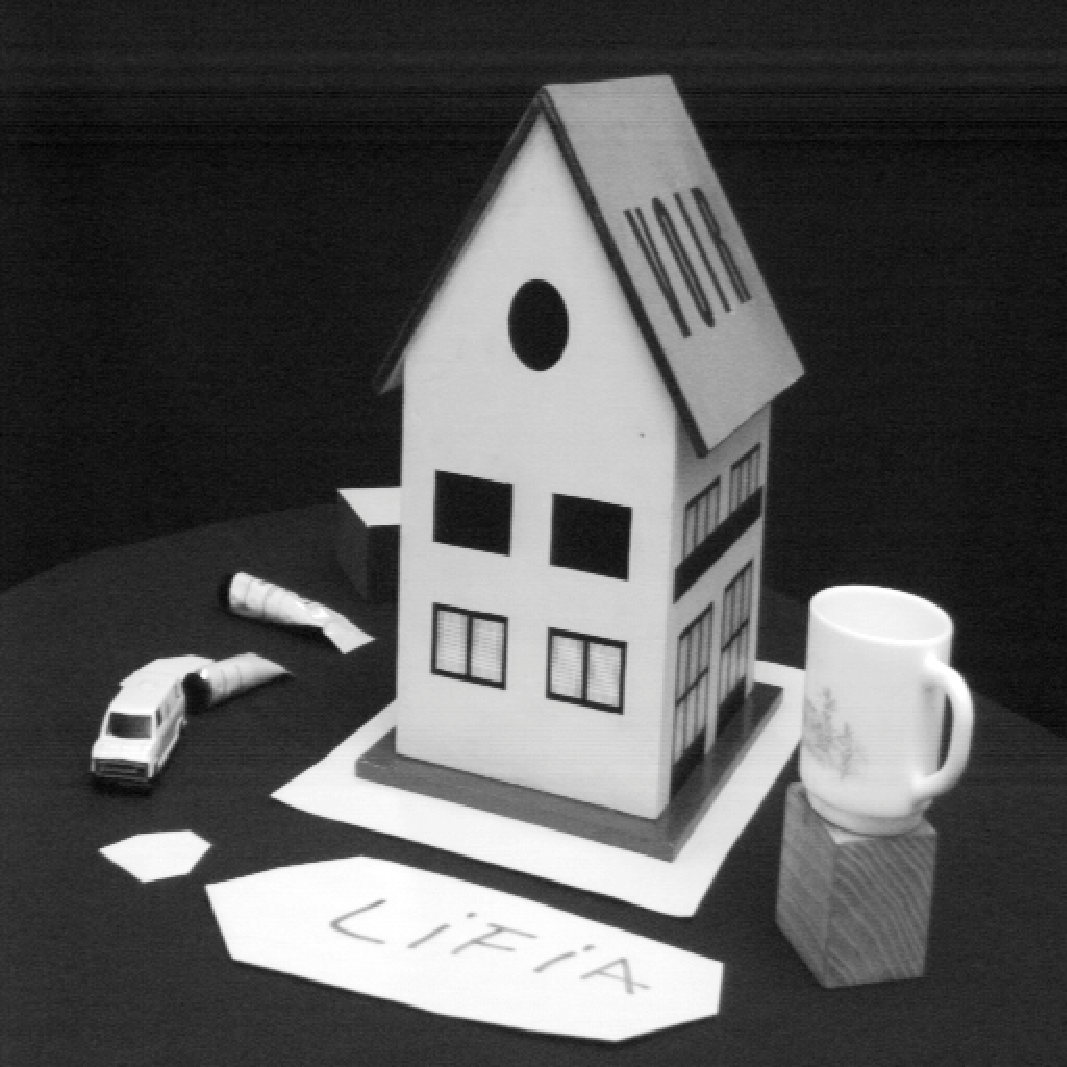
\includegraphics[width= 0.5\columnwidth]{Chapter3/figures/house1} & 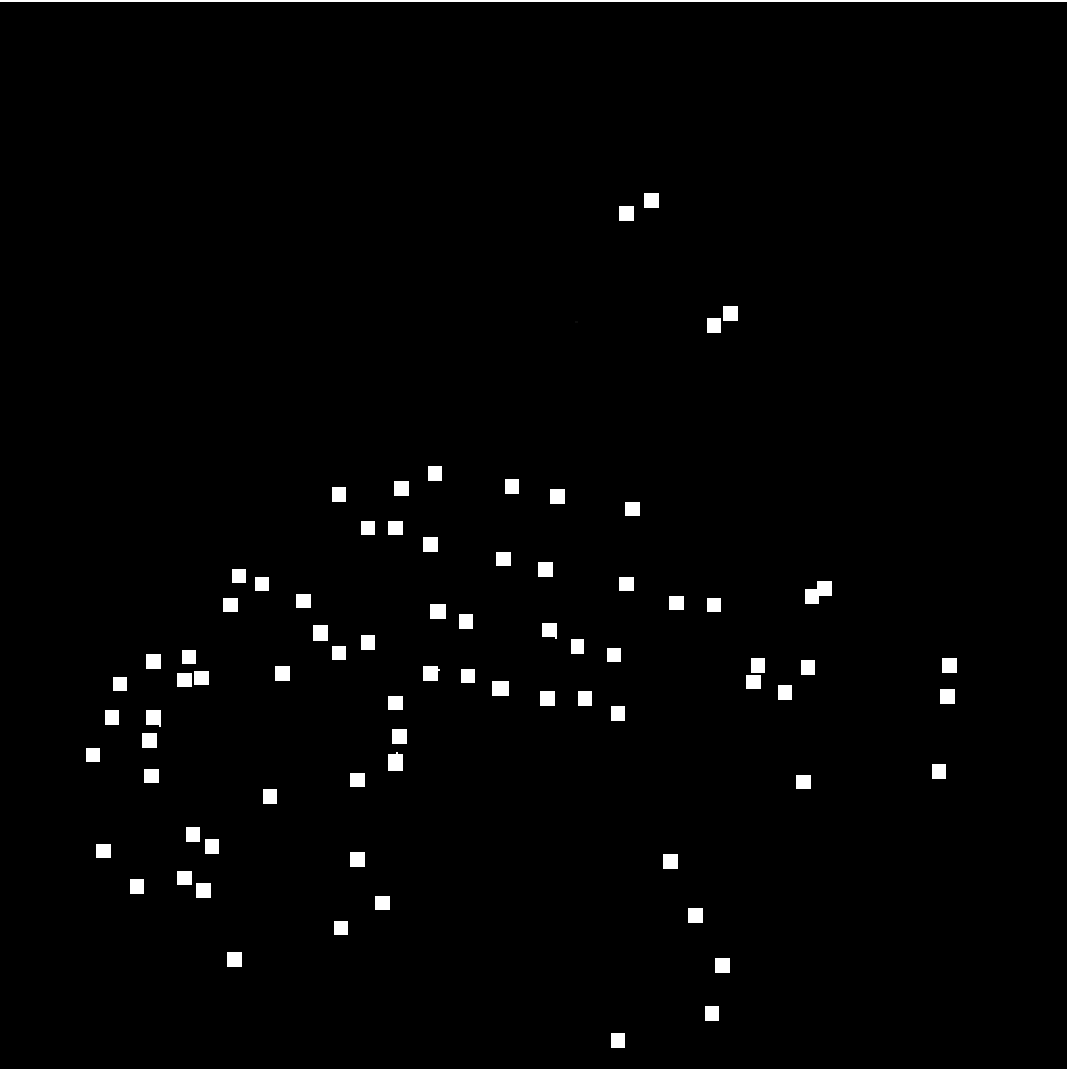
\includegraphics[width= 0.5\columnwidth]{Chapter3/figures/house_harris_map}
	\end{tabular}
	\caption{Illustration de la d�tection de points d'int�r�ts sur une image niveaux de gris 512$\times$512}
	\label{fig_house}
\end{figure}

\subsection{D�tails de l'Impl�mentation}
\begin{figure}[!htb]
	\centering
	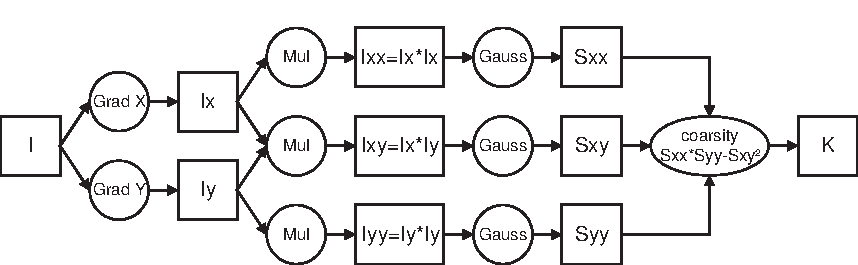
\includegraphics[width= \columnwidth]{Chapter3/figures/harris_NB}
	\caption{Impl�mentation de l'algorithme de Harris sous forme de graphe flot de donn�es}
	\label{fig_HarrisAlgorithm}
\end{figure}
Les images en niveaux de gris sont typiquement des donn�es stock�es une des entiers 8-bit non sign�s et la sortie de l'algorithme de Harris est dans ce cas l� un entier 32 bit sign�. Toutefois, pour des raisons de limitation du jeux d'instruction du SPU, et afin de garantir une comparaison objective avec les extension Altivec et SSE nous avons choisi le format flottant simple pr�cision pour l'entr�e et la sortie de l'algorithme. Dans notre impl�mentation nous avons divis� l'algorithme en 4 noyaux de traitement : un op�rateur de \emph{Sobel} qui repr�sente la d�riv�e dans les directions horizontale et verticale, un op�rateur de multiplication, un noyau de lisage de \emph{Gauss} ($w$ dans l'�quation \ref{eq_03} suivi d'un op�rateur de coarsit�. Nous avons fix� la constante $k$ � z�ro (typiquement elle est fix�e � 0.04) car ceci n'avait pas d'influence sur le r�sultat qualitatif. On obtient ainsi le graphe flot de donn�es donn� dans la figure \ref{fig_HarrisAlgorithm} qui est repr�sentatif d'un algorithme de traitement d'images bas niveau car il englobe des noyaux de convolution et des op�rateurs point � point. Les noyaux de convolution de Sobel ($GradX$ et $GradY$)et le noyau de $Gauss$ sont d�finis comme suit: 
\begin{eqnarray*}
Grad_{X} = \begin{bmatrix}-1 & 0 & 1 \\ -2 & 0 & 2 \\ -1 & 0 & 1 \end{bmatrix}; Grad_{Y} = \begin{bmatrix}-1 & -2 & -1 \\ 0 & 0 & 0 \\ 1 & 2 & 1 \end{bmatrix}; Gauss = \frac{1}{16}\begin{bmatrix}1 & 2 & 1 \\ 2 & 4 & 2 \\ 1 & 2 & 1 \end{bmatrix}
\end{eqnarray*}
\'Etant donn�e qu'ils consomment plus d'entr�es qu'ils ne produisent de sorties, les noyaux de convolution sont le goulot d'�tranglement de l'algorithme car elles augmentent consid�rablement le trafic m�moire. Au vu de la nature des calculs effectu�s dans les diff�rents noyaux, et qui sont tr�s simples g�n�ralement (une suite de multiplications/accumulation) on peut consid�rer que les instructions m�moire sont pr�pond�rantes dans l'application et que de ce fait, on peut qualifier l'algorithme de \emph{memory-bounded problem} (probl�me limit� par la m�moire). C'est pour cela que les efforts d'optimisation sur l'algorithme de Harris sont faites par l'optimisation des acc�s m�moire � diff�rent niveaux de la hi�rarchie m�moire du processeur Cell. 
\section{Exploitation du Parall�lisme et Optimisations Multi-niveau}
Les techniques d'optimisation d�montr�es ici sont multiples et vari�es. Certaines sont de nature algorithmique et rel�vent plut�t du domaine du traitement du signal et des images. D'autres techniques g�n�riques rel�vent plut�t du domaine de l'optimisation logicielle est qu'on retrouve parfois dans certains compilateurs optimisants. Les techniques pr�c�dentes sont g�n�rales et peuvent �tre appliqu�s � la majorit� des processeurs g�n�ralistes car elle ne tiennent pas compte des aspects sp�cifiques d'une architecture donn�e. Par contre, des optimisations de plus haut niveau et qui sont sp�cifiques � l'architecture particuli�re du Cell ont aussi �t� employ�es. Celles-ci ne sont g�n�ralement pas reproductibles sur d'autres architectures parall�les car elles rel�vent plus d'une ad�quation entre l'algorithme et l'architecture qui contient certains dispositifs qui n'existent que sur le Cell et des fois elles r�sultent de contraintes de programmation sp�cifiques au Cell comme la taille limit�e des m�moire locale des SPEs et par cons�quent la gestion logicielle de l'utilisation de la m�moire.
\subsection{Techniques Sp�cifiques au Domaine}
Ces optimisations rel�vent plut�t du domaine du traitement du signal et des images. Elles peuvent donc �tre appliqu�es � plusieurs algorithmes et sur n'importe quelle architecture. Celles que nous avons utilis� concernent les noyaux de convolution et sont : la s�parabilit�, le chevauchement (\emph{overlapping}) et la factorisation des calculs.
\subsubsection{S�parabilit� des Noyaux}
\begin{figure}[!htb]
	\centering
	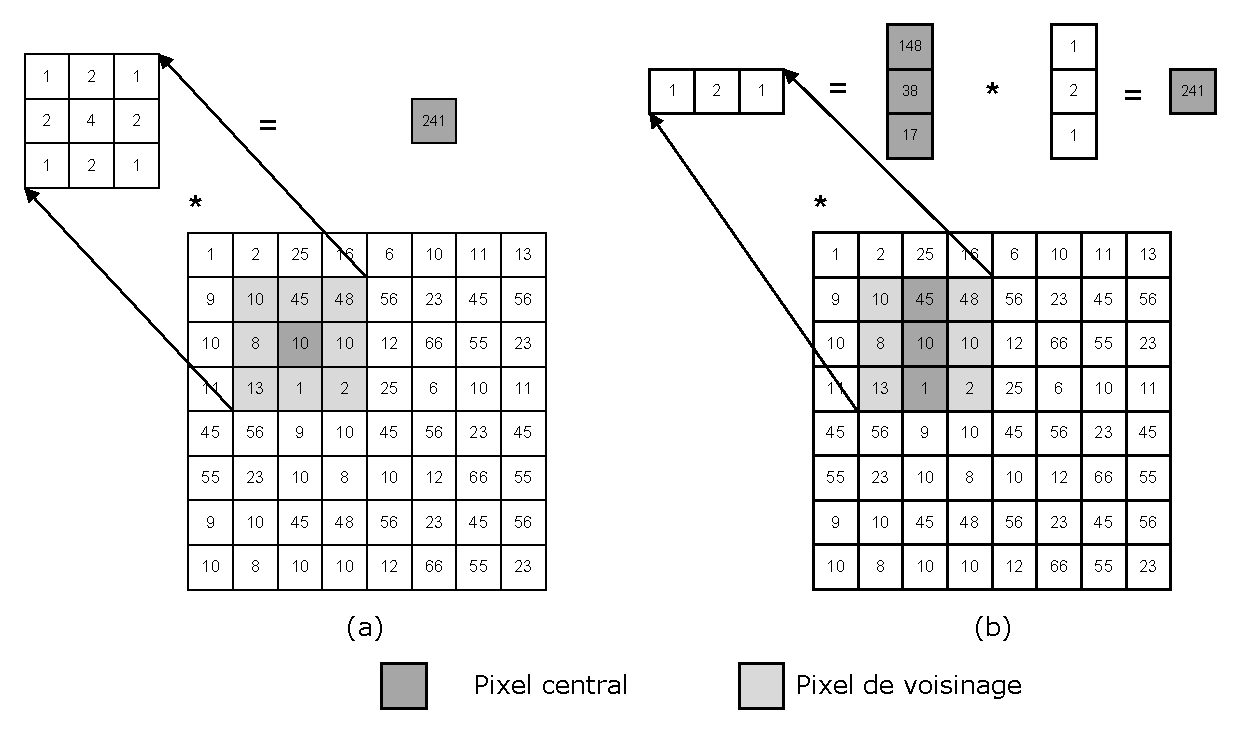
\includegraphics[width= \columnwidth]{Chapter3/figures/convolution_sep}
	\caption{Exemple de convolution par un filtre Gaussien $3\times3$ (a)version avec noyaux 2D (b) version avec deux noyaux 1D , r�sultant de la s�paration du noyau 2D.}
	\label{fig_convosep}
\end{figure}
Cette optimisation consiste � exploiter le fait que les noyaux de convolution 2D de \emph{Sobel} \emph{Gauss} soient s�parables en deux filtre de convolution 1D (Fig. \ref{fig_convosep}). Ainsi, la matrice des coefficients peut �tre exprim�e comme un produit de deux vecteur comme l'illustre les �quations ci-dessous :
\begin{eqnarray*}
Grad_{X} =  \frac{1}{  8} \begin{bmatrix} -1 &  0 &   1  \\ -2 & 0 & 2 \\ -1 & 0 & 1 \end{bmatrix} =    \frac{1}{8} \begin{bmatrix} -1 \\ 0 \\ 1 \end{bmatrix} \times  \begin{bmatrix} 1 & 2 & 1 \end{bmatrix};
Grad_{Y} =  \frac{1}{  8} \begin{bmatrix} -1 & -2 & -1   \\  0 & 0 & 0 \\  1 & 2 & 1 \end{bmatrix}  =   \frac{1}{8} \begin{bmatrix} 1 \\ 2 \\ 1 \end{bmatrix} \times  \begin{bmatrix} -1 & 0 & 1 \end{bmatrix}\\
Gauss      =  \frac{1}{16} \begin{bmatrix}  1 &  2 &   1  \\  2 & 4 & 2 \\  1 & 2 & 1 \end{bmatrix} = \frac{1}{16}\begin{bmatrix}1 \\ 2 \\ 1 \end{bmatrix} \times \begin{bmatrix}1  & 2 & 1 \end{bmatrix}
\end{eqnarray*}
Lorsque l'on s�pare les noyaux de convolution, le calcul se fait en deux passes : une pour chaque vecteur. Gr�ce � la s�parabilit� des noyaux on arrive � r�duire le nombre d'instructions m�moire ainsi que la complexit� arithm�tique. La comparaison est illustr�e dans les tableaux \ref{tab_sepa_arith} et \ref{tab_sepa_mem}.
\begin{table}
\centering
\begin{tabular}{|c|c|c||c|c|c|c|}
\multicolumn{7}{c}{\textbf{Complexit� arithm�tique filtre de \emph{Sobel}}}\\
\hline
\multicolumn{3}{|c||}{\emph{Sans s�paration du noyau}} & \multicolumn{3}{|c|}{\emph{Avec s�paration du noyau}} & \emph{Gain \%}\\
\hline
\textbf{\texttt{MUL}} & \textbf{\texttt{ADD}} & \textbf{Total}& \textbf{\texttt{MUL}} & \textbf{\texttt{ADD}} & \textbf{Total}  & \multirow{2}{*}{\textbf{75}}\\
\cline{1-6}
 2  & 5 & 7  & 1  & 3 & 4  & \\
\hline
\multicolumn{7}{c}{\textbf{Complexit� arithm�tique filtre de \emph{Gauss}}}\\
\hline
\multicolumn{3}{|c||}{\emph{Sans s�paration du noyau}} & \multicolumn{3}{|c|}{\emph{Avec s�paration du noyau}}  & \emph{Gain \%} \\
\hline
\textbf{\texttt{MUL}} & \textbf{\texttt{ADD}} & \textbf{Total}& \textbf{\texttt{MUL}} & \textbf{\texttt{ADD}} & \textbf{Total} &   \multirow{2}{*}{\textbf{116}} \\
\cline{1-6}
 8  & 5 & 13  & 2  & 4 & 6  &  \\
\hline
\end{tabular}
\label{tab_sepa_arith}
\caption{R�duction de la complexit� arithm�tique par s�parabilit� des noyaux}
\end{table}

\begin{table}
\centering
\begin{tabular}{|c|c|c||c|c|c|c|}
\multicolumn{7}{c}{\textbf{Complexit� m�moire filtre de \emph{Sobel}}}\\
\hline
\multicolumn{3}{|c||}{\emph{Sans s�paration du noyau}} & \multicolumn{3}{|c|}{\emph{Avec s�paration du noyau}} & \emph{Gain \%}\\
\hline
\textbf{\texttt{LOAD}} & \textbf{\texttt{STORE}} & \textbf{Total}& \textbf{\texttt{LOAD}} & \textbf{\texttt{STORE}} & \textbf{Total}  & \multirow{2}{*}{\textbf{0}}\\
\cline{1-6}
 6  & 1 & 7  & 1  & 5 & 2  & \\
\hline
\multicolumn{7}{c}{\textbf{Complexit� m�moire filtre de \emph{Gauss}}}\\
\hline
\multicolumn{3}{|c||}{\emph{Sans s�paration du noyau}} & \multicolumn{3}{|c|}{\emph{Avec s�paration du noyau}}  & \emph{Gain \%} \\
\hline
\textbf{\texttt{LOAD}} & \textbf{\texttt{STORE}} & \textbf{Total}& \textbf{\texttt{LOAD}} & \textbf{\texttt{STORE}} & \textbf{Total} &   \multirow{2}{*}{\textbf{25}} \\
\cline{1-6}
 9  & 1 & 10  & 6  & 1 & 8  &  \\
\hline
\end{tabular}
\label{tab_sepa_mem}
\caption{R�duction de la complexit� m�moire par s�parabilit� des noyaux}
\end{table}

\subsubsection{Chevauchement des Noyaux}
\begin{figure}[!htb]
	\centering
	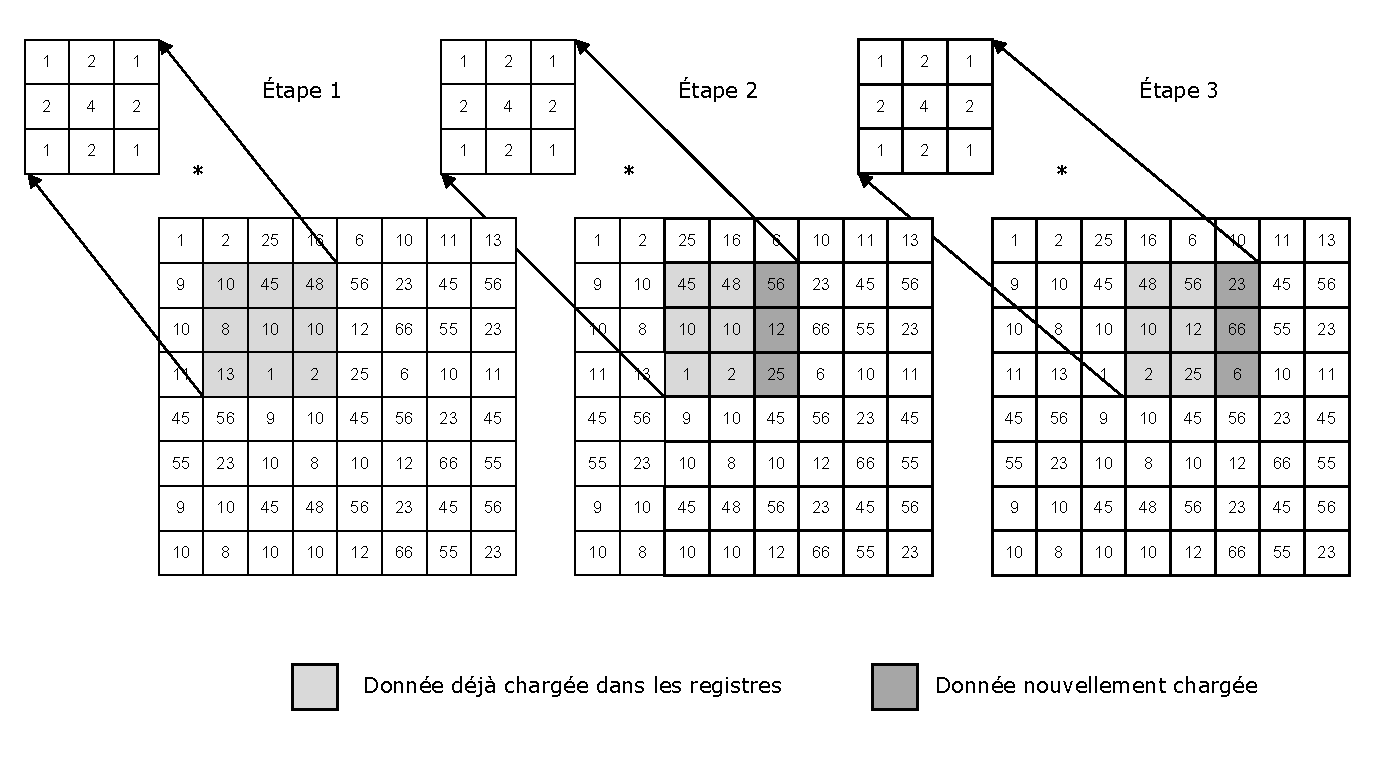
\includegraphics[width= \columnwidth]{Chapter3/figures/convolution_overlap}
	\caption{Chevauchement des donn�es pour un calcul d'un filtre Gaussien $3\times3$, certaines donn�es sont conserv�es en d�calant le masque de convolution.}
	\label{fig_convoover}
\end{figure}
La deuxi�me particularit� des noyaux de convolution est une notion de chevauchement qui permet d'avoir une redondance d'une partie des donn�es (Fig. \ref{fig_convoover}). En effet, comme le d�montre la figure \ref{fig_ovelapping}, � chaque it�ration du calcul de la convolution il n'y a qu'une seule nouvelle colonne charg�e. Les colonnes redondantes sont copi�es dans les registres en les d�calant d'un pas � droite par rapport � leur position pr�c�dente (\emph{rotation de registres}). On notera que le m�me type d'optimisation peut se faire gr�ce � un \emph{d�roulage de boucle}.
\begin{table}
\centering
\begin{tabular}{|c|c|c||c|c|c|c|}
\multicolumn{7}{c}{\textbf{Complexit� m�moire filtre de \emph{Sobel}}}\\
\hline
\multicolumn{3}{|c||}{\emph{Sans chevauchement du noyau}} & \multicolumn{3}{|c|}{\emph{Avec chevauchement du noyau}} & \emph{Gain \%}\\
\hline
\textbf{\texttt{LOAD}} & \textbf{\texttt{STORE}} & \textbf{Total}& \textbf{\texttt{LOAD}} & \textbf{\texttt{STORE}} & \textbf{Total}  & \multirow{2}{*}{\textbf{133}}\\
\cline{1-6}
 6  & 1 & 7  & 2  & 1 & 3  & \\
\hline
\multicolumn{7}{c}{\textbf{Complexit� m�moire filtre de \emph{Gauss}}}\\
\hline
\multicolumn{3}{|c||}{\emph{Sans chevauchement du noyau}} & \multicolumn{3}{|c|}{\emph{Avec chevauchement du noyau}}  & \emph{Gain \%} \\
\hline
\textbf{\texttt{LOAD}} & \textbf{\texttt{STORE}} & \textbf{Total}& \textbf{\texttt{LOAD}} & \textbf{\texttt{STORE}} & \textbf{Total} &   \multirow{2}{*}{\textbf{150}} \\
\cline{1-6}
 9  & 1 & 10  & 3  & 1 & 4  &  \\
\hline
\end{tabular}
\label{tab_over_mem}
\caption{R�duction de la complexit� m�moire par chevauchement des noyaux}
\end{table}
\subsubsection{S�paration des noyaux et chevauchement}
Cette optimisation n'est en fait qu'une combinaison des deux pr�c�dentes. En effet on profite d'une part du fait que les noyaux soient s�parables pour r�duire la complexit� arithm�tique, et d'autre part du chevauchement des noyaux pour m�moriser le r�sultat pr�c�dent. Ainsi, au lieu de m�moriser les deux derni�res colonnes, on m�morise le r�sultat du filtrage par le premier filtre 1D pour le r�utiliser � l'it�ration suivante de la boucle. Dans ce cas l�; la compl�xit� arithm�tique est la m�me que celle de la version avec s�paration des noyaux, alors que la complexit� m�moire est r�duite d'avantage.
Les tableau \ref{tab_sepaover_arith} et \ref{tab_sepaover_mem} donnent la diff�rence en terme de complexit� arithm�tique et m�moire entre la version de base de l'algorithme est la version tenant compte des deux optimisations combin�es.
\begin{table}
\centering
\begin{tabular}{|c|c|c||c|c|c|c|}
\multicolumn{7}{c}{\textbf{Complexit� arithm�tique filtre de \emph{Sobel}}}\\
\hline
\multicolumn{3}{|c||}{\emph{Sans s�paration du noyau + chevauchement}} & \multicolumn{3}{|c|}{\emph{Avec s�paration du noyau + chevauchement}} & \emph{Gain \%}\\
\hline
\textbf{\texttt{MUL}} & \textbf{\texttt{ADD}} & \textbf{Total}& \textbf{\texttt{MUL}} & \textbf{\texttt{ADD}} & \textbf{Total}  & \multirow{2}{*}{\textbf{75}}\\
\cline{1-6}
 2  & 5 & 7  & 1  & 3 & 4  & \\
\hline
\multicolumn{7}{c}{\textbf{Complexit� arithm�tique filtre de \emph{Gauss}}}\\
\hline
\multicolumn{3}{|c||}{\emph{Sans s�paration du noyau + chevauchement}} & \multicolumn{3}{|c|}{\emph{Avec s�paration du noyau + chevauchement}}  & \emph{Gain \%} \\
\hline
\textbf{\texttt{MUL}} & \textbf{\texttt{ADD}} & \textbf{Total}& \textbf{\texttt{MUL}} & \textbf{\texttt{ADD}} & \textbf{Total} &   \multirow{2}{*}{\textbf{116}} \\
\cline{1-6}
 8  & 5 & 13  & 2  & 4 & 6  &  \\
\hline
\end{tabular}
\label{tab_sepaover_arith}
\caption{R�duction de la complexit� arithm�tique par s�parabilit� et chevauchement des noyaux}
\end{table}

\begin{table}
\centering
\begin{tabular}{|c|c|c||c|c|c|c|}
\multicolumn{7}{c}{\textbf{Complexit� m�moire filtre de \emph{Sobel}}}\\
\hline
\multicolumn{3}{|c||}{\emph{Sans s�paration du noyau + chevauchement}} & \multicolumn{3}{|c|}{\emph{Avec s�paration du noyau + chevauchement }} & \emph{Gain \%}\\
\hline
\textbf{\texttt{LOAD}} & \textbf{\texttt{STORE}} & \textbf{Total}& \textbf{\texttt{LOAD}} & \textbf{\texttt{STORE}} & \textbf{Total}  & \multirow{2}{*}{\textbf{250}}\\
\cline{1-6}
 6  & 1 & 7  & 1  & 1 & 2  & \\
\hline
\multicolumn{7}{c}{\textbf{Complexit� m�moire filtre de \emph{Gauss}}}\\
\hline
\multicolumn{3}{|c||}{\emph{Sans s�paration du noyau + chevauchement}} & \multicolumn{3}{|c|}{\emph{Avec s�paration du noyau + chevauchement }}  & \emph{Gain \%} \\
\hline
\textbf{\texttt{LOAD}} & \textbf{\texttt{STORE}} & \textbf{Total}& \textbf{\texttt{LOAD}} & \textbf{\texttt{STORE}} & \textbf{Total} &   \multirow{2}{*}{\textbf{400}} \\
\cline{1-6}
 9  & 1 & 10  & 1  & 1 & 2  &  \\
\hline
\end{tabular}
\label{tab_sepaover_mem}
\caption{R�duction de la complexit� m�moire par s�parabilit� et chevauchement des noyaux}
\end{table}
\subsubsection{Composition de Fonctions}
\label{sectioncompo}
\begin{figure}[!htb]
	\centering
  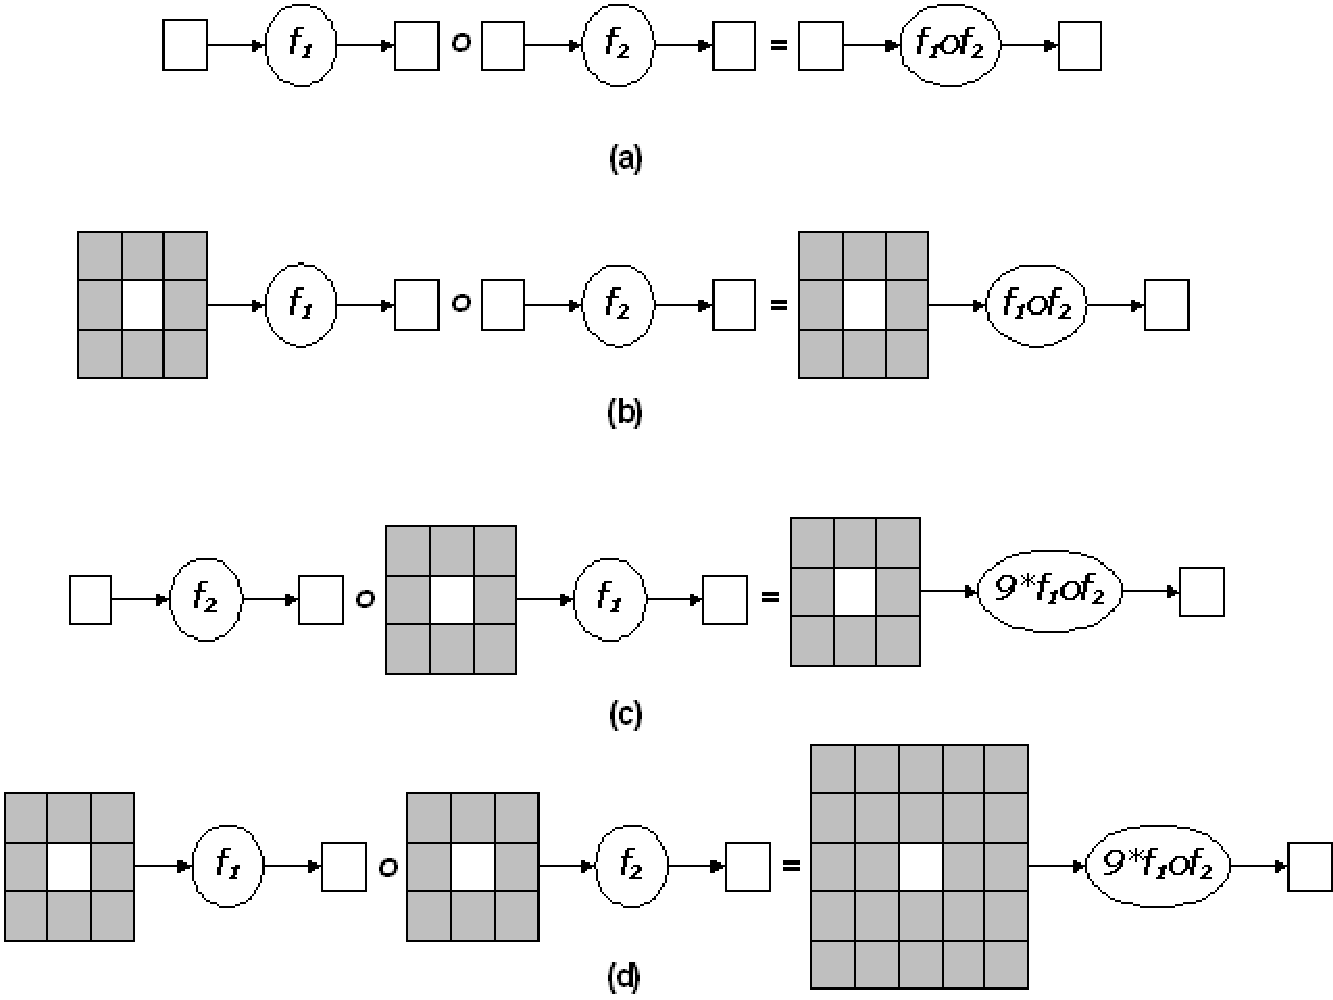
\includegraphics[width= \columnwidth]{Chapter3/figures/funccompo}
  	\label{fig_compo}
	\caption{R�gle de composition de fonctions.\textbf{(a)} composition de deux op�rateurs point � point \textbf{(b)} composition d'un noyaux de convolution suivi d'un op�rateur point � point \textbf{(c)} composition d'un op�rateur point � point  suivi d'un noyaux de convolution \textbf{(d)} composition de deux noyaux de convolution successifs}
\end{figure}

Cette technique d'optimisation s'av�re tr�s efficace surtout dans les codes ou les instructions m�moire sont pr�pond�rantes. En effet, le fait de composer deux fonctions de calcul pour en faire une seule qui effectue les deux calculs r�duit consid�rablement le nombre d'acc�s m�moire puisque les op�rations de sauvegarde et de chargement interm�diaires entre les deux fonctions initiales sont supprim�es, et la transaction se fait au niveaux des registres. De plus, le cout de l'appel de fonction (taille de la pile, et branchement) est �galement r�duit, car le r�sultat de la composition de fonctions et une seule fonction. Dans les cas les plus simples, la mise en oeuvre de cette technique n'est pas difficile. Toutefois, lorsqu'il s'agit d'op�rateurs de convolution comme dans notre cas, des nouvelles contraintes apparaissent afin de garantir la validit� du r�sultat du calcul. Ainsi, des r�gles de composition s'imposent en fonction de l'ordre dans lequel s'enchainent les fonctions. Ces r�gles sont illustr�es sur la figure \ref{fig_compo}. On peut alors constater qu'il existe plusieurs r�gles de composition des fonctions selon d'une part, la nature des op�rateurs mis en jeu et d'autre part l'ordre dans lequel il s'enchainent. En terme d'apport de cette technique en terme de performances nous observons deux aspects distincts:
\begin{itemize}
\item \textbf{Complexit� m�moire} : on observe en effet que ceux ci sont syst�matiquement r�duits, car les op�rations de \texttt{LOAD/STORE} interm�diaires sont supprim�s, sauf dans le cas de la composition de deux noyaux de convolution (cas \textbf{(d)} sur la figure \ref{fig_compo})ou la pr�sence de bords suppl�mentaires augmente consid�rablement le nombre des acc�s m�moire.
\item \textbf{Complexit� arithm�tique} : Celle-ci ne change pas dans le meilleurs des cas notamment lorsque les op�rateurs compos�es sont point � point ou alors lorsque l'op�rateur de convolution est plac� devant un op�rateur point � point (cas \textbf{(b)} sur la figure \ref{fig_compo}). Toutefois, si la convolution est plac�e � la suite d'un quelconque traitement, elle impose que l'op�rateur qui la pr�c�de soit effectu� sur tous les pixels de voisinage, ce qui augmente consid�rablement la complexit� arithm�tique, en particulier lorsque l'op�rateur qui pr�c�de est une convolution (cas \textbf{(d)} sur la figure \ref{fig_compo}).
\end{itemize}
D'apr�s les observations ci-dessus, la composition de fonction peut �tre un bon choix pour l'optimisation d'une cha�ne de traitement telle que l'algorithme de d�tection de point d'int�r�ts de Harris. Toutefois, toutes les combinaisons n'apportent pas forc�ment une am�lioration des performances, elle peuvent m�me dans certains cas les d�grader. Le tableau \ref{tab_memall} r�sume les complexit� m�moire et arithm�tiques des diff�rents cas de composition sur la figure \ref{fig_compo} en incluant �galement les optimisations d�crites auparavant.
\begin{table}
\centering
\begin{tabular}{|c||c|c|c|c|}
\hline
\multicolumn{5}{|c|}{\textbf{Version de base sans composition}}\\
\hline
\textbf{Op�rateur} & \textbf{Occurrences} & \textbf{\texttt{LOADS}} & \textbf{\texttt{STORE}} & \textbf{Total}\\
\hline
\emph{Sobel} & 2 & 6 & 1 & 14\\
\hline
\emph{Mul} & 3 & 2 & 1 & 9\\
\hline
\emph{Gauss} & 3 & 9 & 1 & 30\\
\hline
\emph{Coarsity} & 1 & 3 & 1 & 4\\
\hline
\emph{Harris} & 1 & 48 & 9 & 57\\
\hline
\multicolumn{5}{|c|}{\textbf{Version avec chevauchement et s�paration des noyaux sans composition}}\\
\hline
\textbf{Op�rateur} & \textbf{Occurrences} & \textbf{\texttt{LOADS}} & \textbf{\texttt{STORE}} & \textbf{Total}\\
\hline
\emph{Sobel} & 1 & 3 & 2 & 5\\
\hline
\emph{Mul} & 3 & 2 & 1 & 6\\
\hline
\emph{Gauss} & 3 & 3 & 1 & 12\\
\hline
\emph{Coarsity} & 1 & 3 & 1 & 4\\
\hline
\emph{Harris} & 1 & 21 & 9 & 30\\
\hline
\multicolumn{5}{|c|}{\textbf{Version avec composition de Sobel$\circ$Mul et Gauss$\circ$Coarsity}}\\
\hline
\textbf{Op�rateur} & \textbf{Occurrences} & \textbf{\texttt{LOADS}} & \textbf{\texttt{STORE}} & \textbf{Total}\\
\hline
\emph{Sobel$\circ$Mul} & 1 & 9 & 3 & 12\\
\hline
\emph{Gauss$\circ$Coarsity} & 3 & 9 & 1 & 28\\
\hline
\emph{Harris} & 1 & 36 & 4 & 40\\
\hline
\multicolumn{5}{|c|}{\textbf{Version avec chevauchement et s�paration + composition de Sobel$\circ$Mul et Gauss$\circ$Coarsity}}\\
\hline
\textbf{Op�rateur} & \textbf{Occurrences} & \textbf{\texttt{LOADS}} & \textbf{\texttt{STORE}} & \textbf{Total}\\
\hline
\emph{Sobel$\circ$Mul} & 1 & 3 & 3 & 6\\
\hline
\emph{Gauss$\circ$Coarsity} & 3 & 3 & 1 & 10\\
\hline
\emph{Harris} & 1 & 12 & 4 & 16\\
\hline
\multicolumn{5}{|c|}{\textbf{Version avec composition de Sobel$\circ$Mul$\circ$Gauss$\circ$Coarsity}}\\
\hline
\textbf{Op�rateur} & \textbf{Occurrences} & \textbf{\texttt{LOADS}} & \textbf{\texttt{STORE}} & \textbf{Total}\\
\hline
\emph{Sobel$\circ$Mul$\circ$Gauss$\circ$Coarsity} & 1 & 25 & 1 & 26\\
\hline
\emph{Harris} & - & - & - & 26\\
\hline
\multicolumn{5}{|c|}{\textbf{Version avec chevauchement et s�paration + composition de Sobel$\circ$Mul$\circ$Gauss$\circ$Coarsity}}\\
\hline
\textbf{Op�rateur} & \textbf{Occurrences} & \textbf{\texttt{LOADS}} & \textbf{\texttt{STORE}} & \textbf{Total}\\
\hline
\emph{Sobel$\circ$Mul$\circ$Gauss$\circ$Coarsity} & 1 & 5 & 1 & 6\\
\hline
\emph{Harris} & - & - & - & 6\\
\hline
\end{tabular}
\label{tab_memall}
\caption{Tableau r�capitulatif de l'optimisation des acc�s m�moire en combinant l'ensemble des optimisations}
\end{table}
\subsection{Optimisation des Transferts M�moire}
\begin{figure}[!htb]
	\centering
  \includegraphics[width= \columnwidth]{Chapter3/figures/cellnoc}
  \label{fignoc}
	\caption{R�seau d'interconnection du Cell}
\end{figure}
Dans cette partie, nous abordons des techniques d'optimisations qui sont relatives au transferts de donn�es pr�sents dans l'application. On entend, par transfert de donn�e, toute communication qui met en jeu deux m�moires physiques sur Cell. Cela comporte les transferts DMA entre la m�moire principale et les m�moires locales des SPEs ainsi que les communications mettant en jeu deux m�moires priv�es de SPEs. Plusieurs aspects sont mis en avant. D'une part, les caract�ristiques internes de l'architecture du r�seaux de communications \cite{cellnoc} (\emph{Network On Chip (NoC)}) du Cell et d'autres part la nature des transferts de donn�es impos�es par l'algorithme et la partition des donn�es � plusieurs niveaux de la hi�rarchie m�moire.
\subsubsection{Optimisation de la Bande-Passante du \emph{NoC}}
Dans le mod�le de programmation utilis� qui est bas� sur le \emph{SDK} du Cell et les librairies \emph{libspe}, les donn�es pr�sentes en m�moire centrale sont transf�r�es aux m�moires locales des SPEs avant d'�tre trait�es. Ces transferts se font d'une mani�re explicite dans le logiciel par appel � des fonctions de l'API de gestion du \emph{MFC} et ils sont g�r�es par le \emph{Noc} au travers de contr�leurs m�moire et de l'arbitre de bus. L'architecture du Bus et la topologie du r�seau impose quelques contraintes qui jouent un r�le primordial dans la minimisation des latences des communications point � point.
\paragraph{Taille du Transfert}
\begin{figure}[htb]
  \centering
  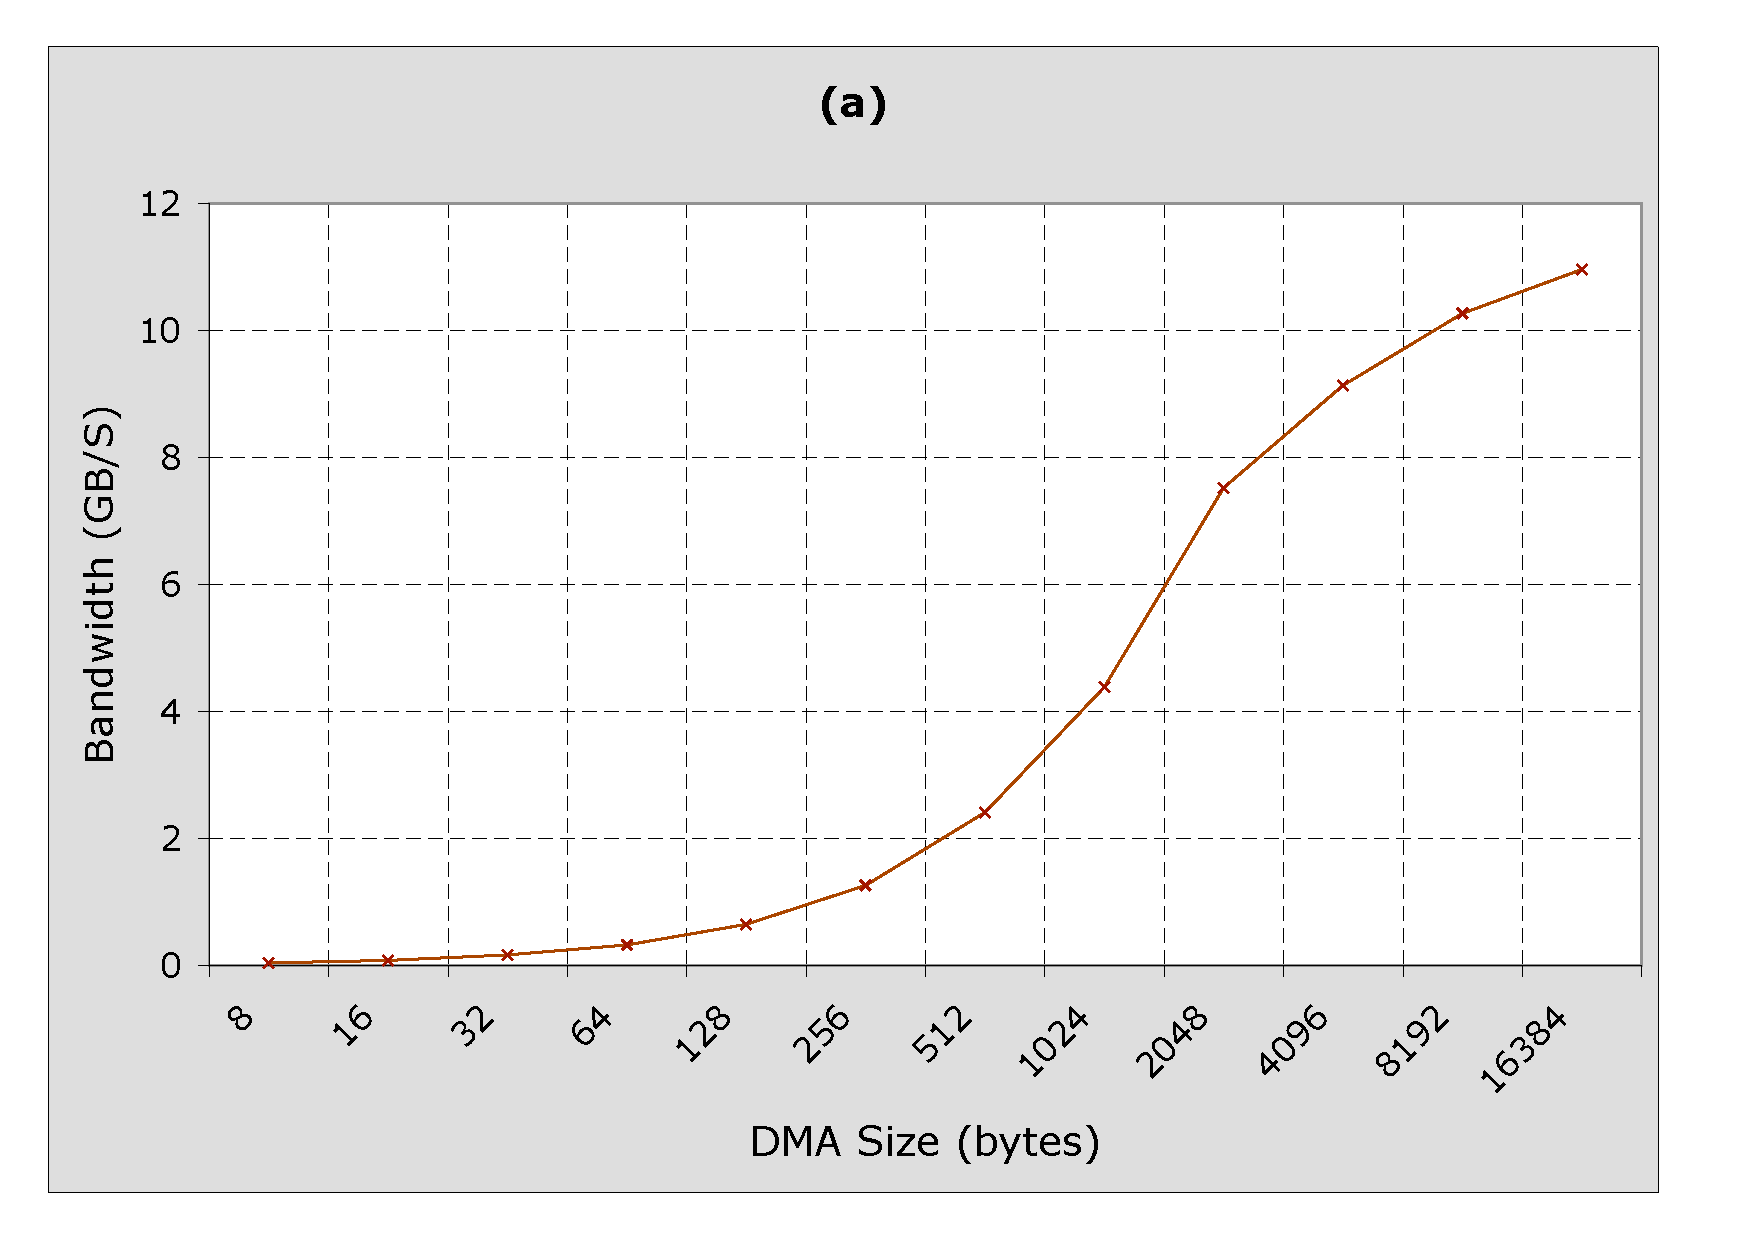
\includegraphics[width= 0.8\columnwidth]{Chapter3/figures/bwsize}
  \label{figbwsize}
  \caption{Influence de la taille du transfert DMA sur la bande-passante}
\end{figure}
%\begin{figure}[!htb]
%	\centering
%  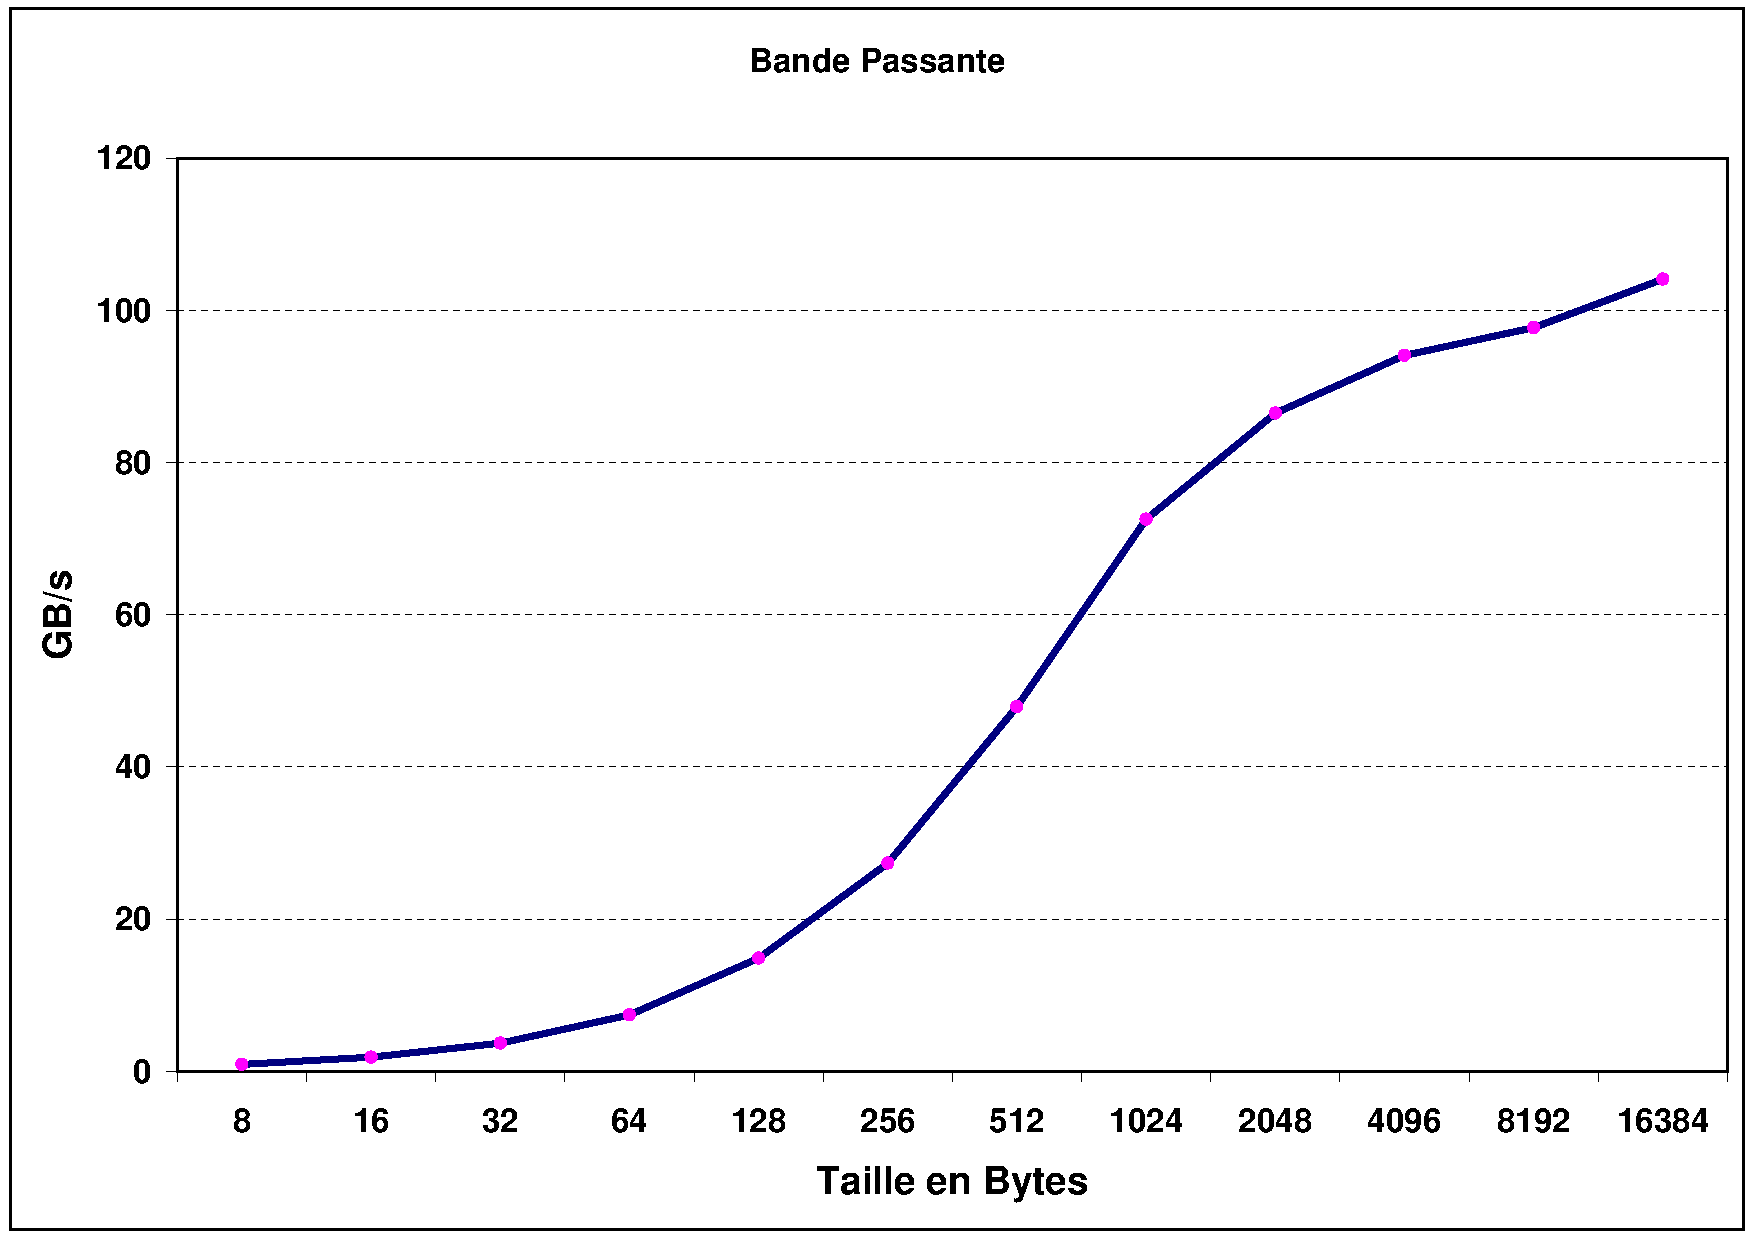
\includegraphics[width= 0.8\columnwidth]{Chapter3/figures/grapheBW}
%  \label{graphbw}
%	\caption{Bande-passante cumul�e }
%\end{figure}

Le premier param�tre influant sur la bande passante est la taille du bloc de donn�es transf�r�. D'une part, il y a des contraintes impos�es par l'API de transfert qui limite les tailles d'un bloc transf�r� par une commande DMA � 1, 2, 4, 8 octets ou tout multiple de 16 \emph{bytes} et la taille de donn�es maximale transf�r�e en une seule commande est de 16 \emph{KB}. Des plus les adresses doivent obligatoirement �tre align�es sur 16 \emph{bytes} et un alignement sur 128 \emph{bytes} est pr�f�rable � cause de la taille de la ligne de cache sur la m�moire locale du SPE qui est de 128 \emph{bytes}. D'autre part l'espace m�moire disponible sur les SPEs pour stocker donn�es et instructions est limit� � 256 KB. Toutes ces contraintes, imposent une attention des contraintes fortes en termes de taille de bloc transf�r� et d'alignement des donn�es qui ne sont pas du ressort du d�veloppeur dans les architectures � m�moire partag�e. Plusieurs \emph{benchmarks} ont �t� effectu�s dans \cite{cellnoc} et \cite{cell_bw02} et qui d�montrent la relation entre la taille et � la fois le d�bit et la latence des transferts sur le Cell. Le graphe \ref{graphbw} donne les r�sultats sur un benchmark de bande-passante que nous avons effectu� sur une BladeCenter QS20 et d�montrent que celle ci est proportionnelle � la taille des donn�es transf�r�es. Ceci s'explique par le fait que la \emph{latence} du transfert qui repr�sente le temps d'initialisation d'un transfert, cette dur�e �tant la m�me quelque soit la taille du paquet jusqu'� 16 KB.
\paragraph{Nombre de Transferts Concurrents}
\begin{figure}[htb]
  \centering
  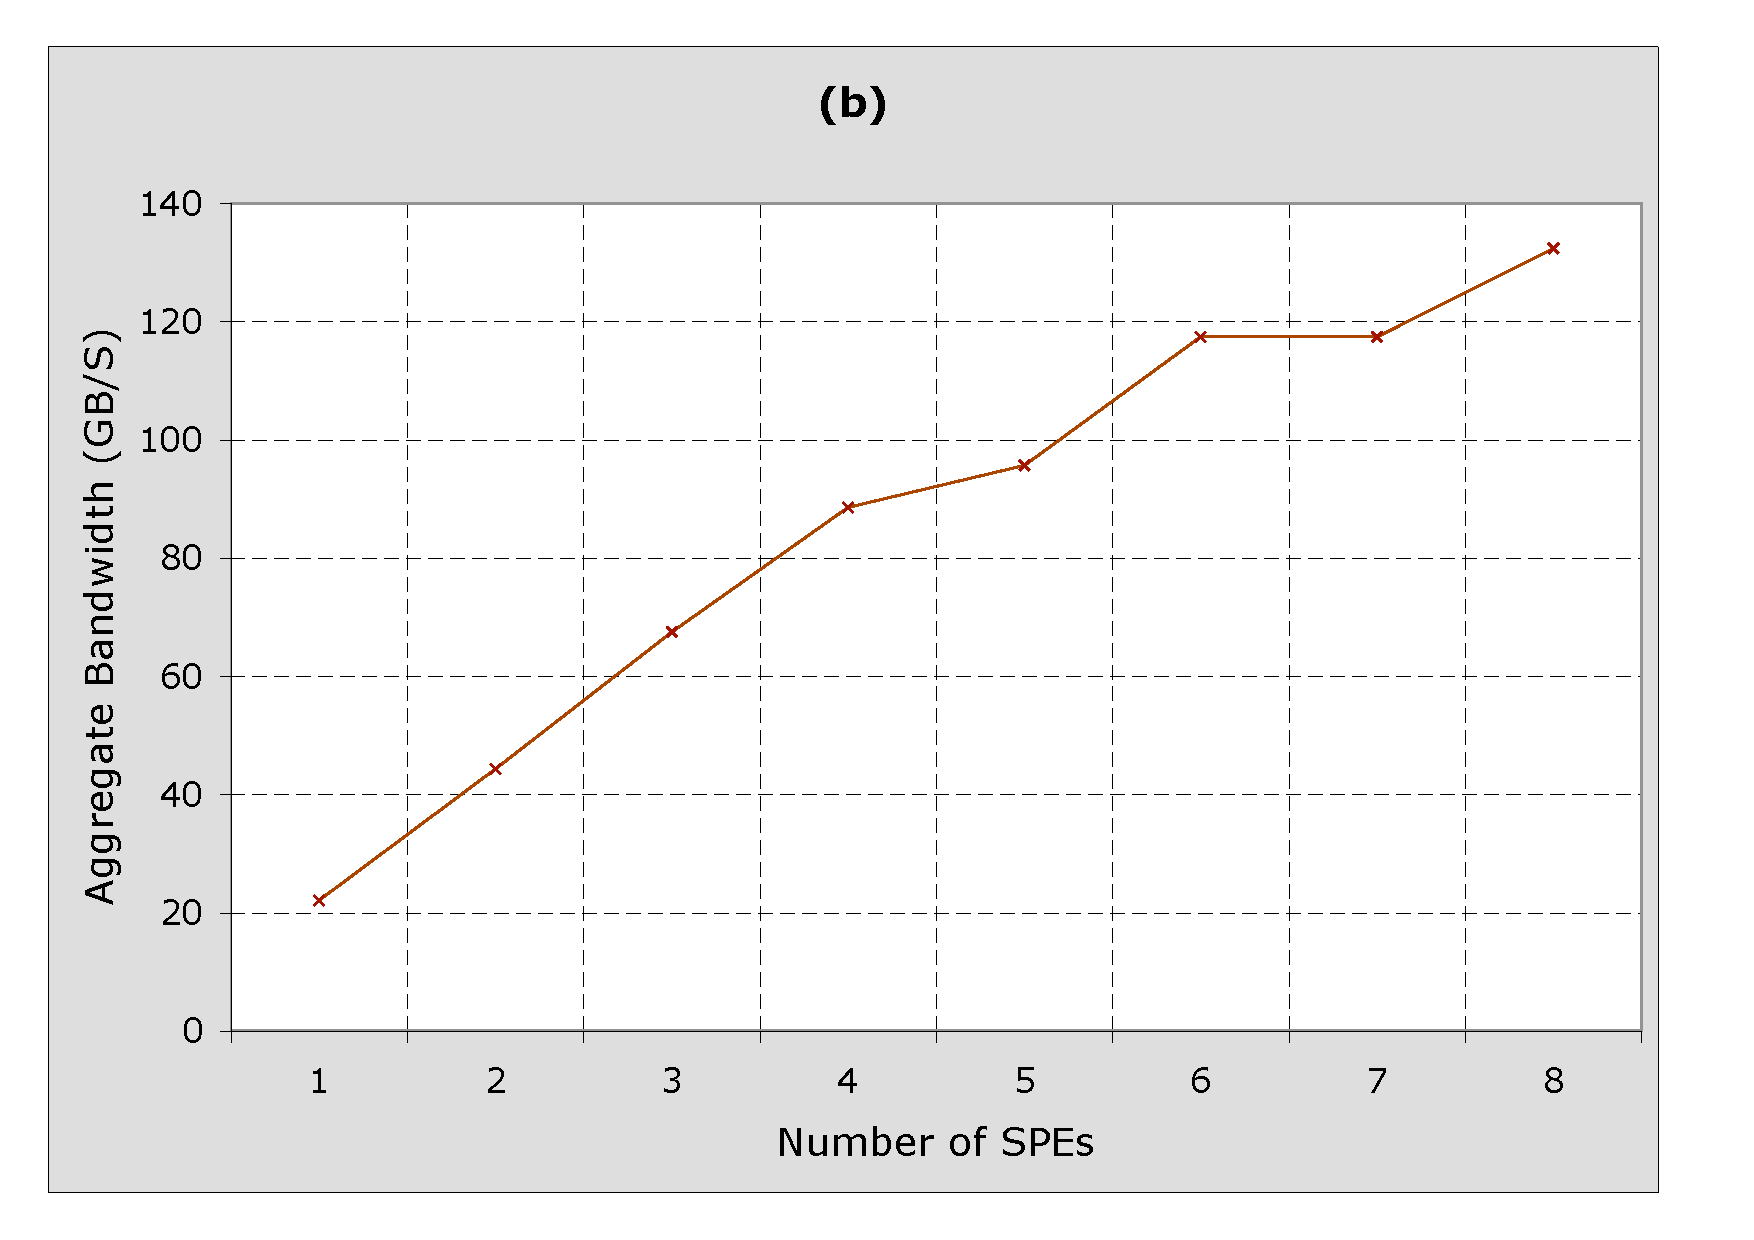
\includegraphics[width= 0.8\columnwidth]{Chapter3/figures/bwcontention}
  \label{figbwncontention}
  \caption{Influence du nombre de transferts dans le cas d'une communication LS<->LS}
\end{figure}

\begin{figure}[htb]
  \centering
  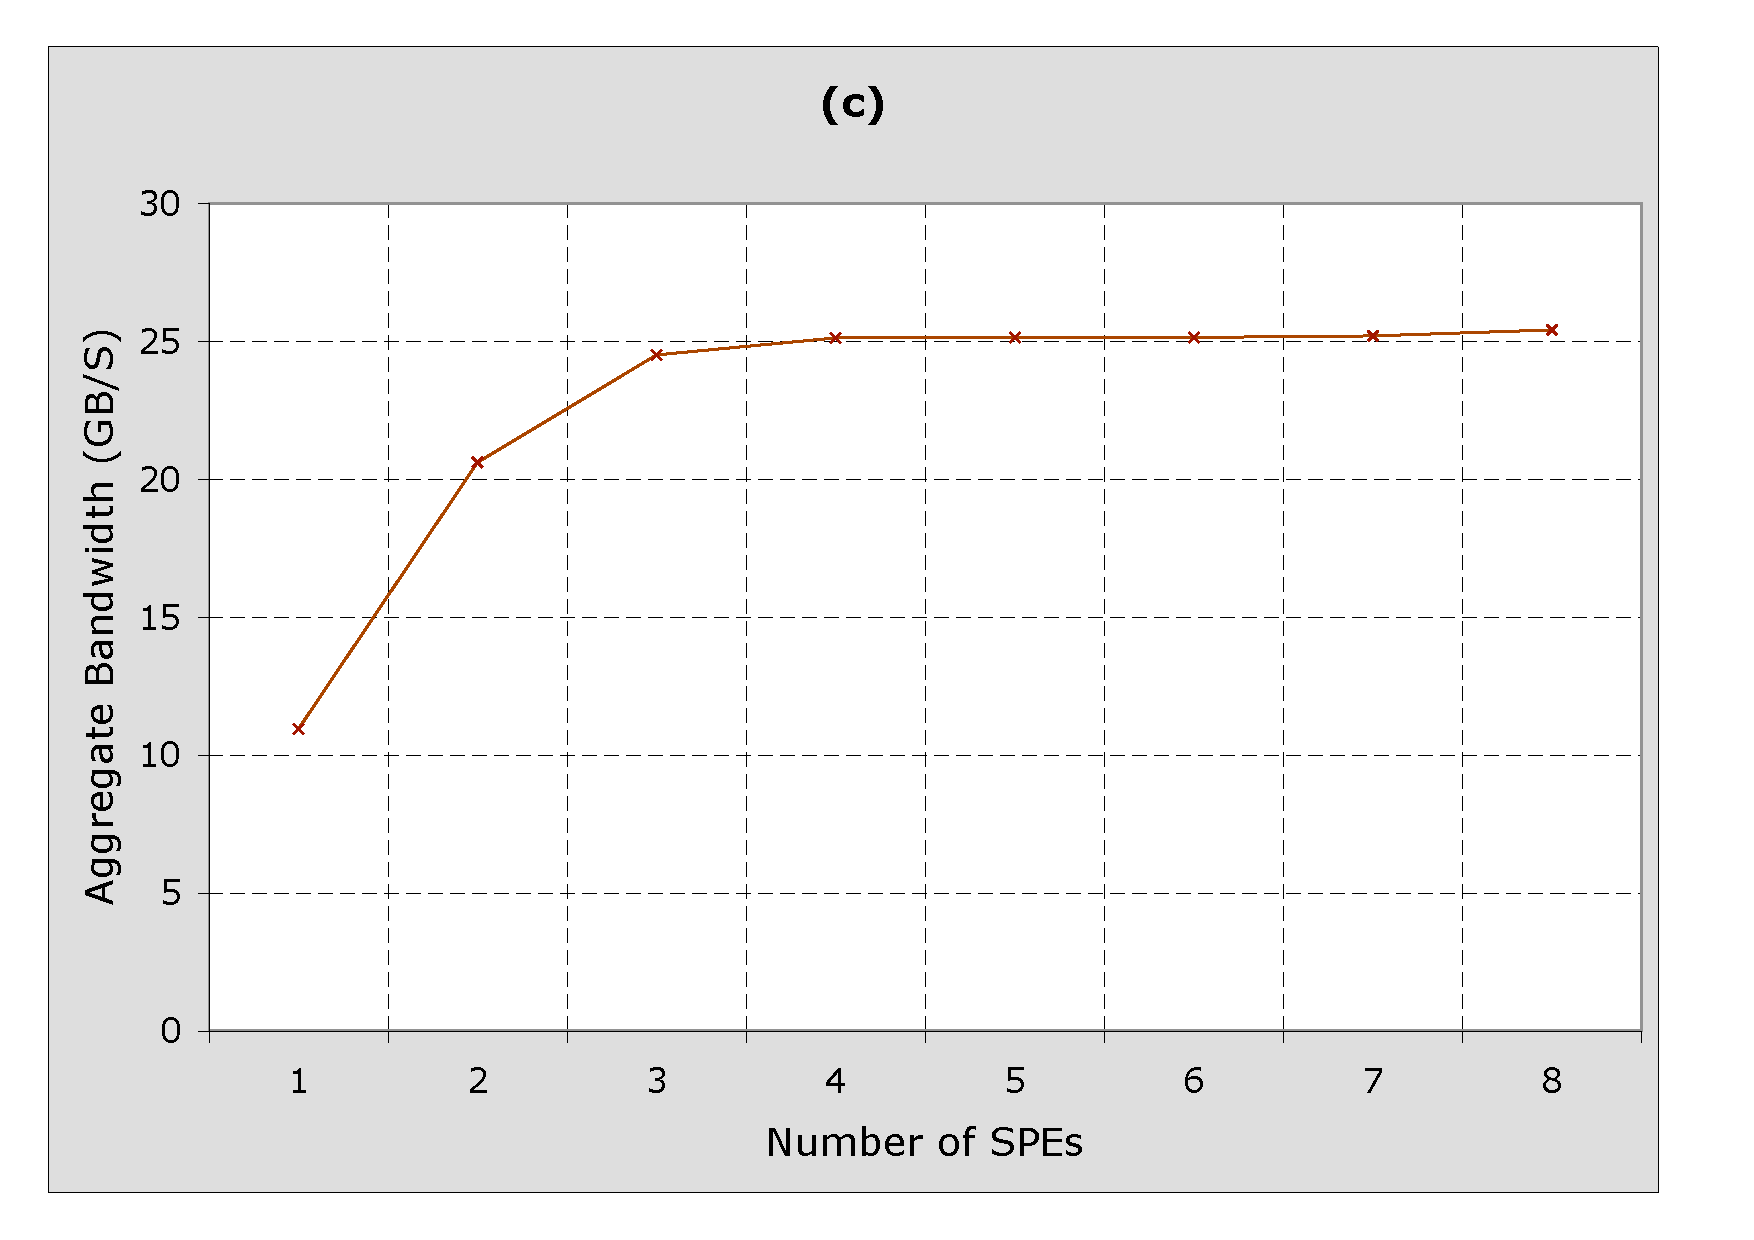
\includegraphics[width= 0.8\columnwidth]{Chapter3/figures/bwnspes}
  \label{figbwnspes}
  \caption{Influence du nombre de transferts dans le cas d'une communication MS<->LS}
\end{figure}

Les second facteur qui influe sur l'efficacit� du r�seau lors des transferts est le nombre de transferts s'ex�cutant en parall�le. En effet, l'architecture du r�seau dont la topologie est tu type \emph{token ring} contient quatre anneaux d'une largeur de 128-bit : deux dans le sens d'une aiguille d'une montre et les deux autres dans le sens contraire. En observant la topologie du r�seau ainsi que le sens de circulation des donn�es sur les anneaux du bus, il s'av�re �vident qu'il peut y avoir collision entre deux transferts s'ex�cutant de mani�re concurrente (\ref{fignoc}). Sachant qu'un anneau peut g�rer 3 transferts concurrents tant que ceux-ci n'entrent pas en collision. Ce risque est d'autant plus important si le nombre de transferts concurrents augmente (au-del� de 12). Lorsqu'un tel conflit est d�tect�,  l'arbitre de bus le r�sout avec un surcout qui divise globalement la bande-passante par deux. La courbe sur le figure \ref{figbwncontention} permet de constater l'influence du nombre de transferts concurrents, on peut ainsi observer que la courbe perd sa lin�arit� quand au del� de 4 SPEs et ceci car le nombre de transferts devient trop important pour ne pas provoquer de collisions sur le bus.\\
\indent Dans le cas d'une communication du PPE vers le SPE, la bande passante maximale qui peut �tre atteinte est de 25.6 GB/s. Dans le cas o� plusieurs SPEs font une requ�te vers la m�moire principale les transferts ne peuvent �tre que s�rialis�s car il existe qu'une seule liaison vers le MS (\emph{Main Storage}). On observe alors que le graphique de la figure \ref{bwnspes} que la bande passante maximale n'est atteinte que lorsqu'au moins 4 SPEs font un transfert de la m�moire centrale vers leurs m�moires priv�e. 

\subsubsection{Optimisation de la localit� temporelle par chainage des op�rateurs}
Le but vis� par cette technique est de rapprocher le plus possible les donn�es des unit�s de traitement. En effet, les couts li�s au transfert des donn�es de la m�moire centrale vers les m�moires locales �tant important, il est pertinent de garder les donn�es en m�moire locale apr�s chaque traitement au lieu de multiplier les lectures/�critures vers la m�moire centrale. Les r�gles de chainage des op�rateurs au niveaux des acc�s m�moires, sont les m�mes que pour la composition des op�rateurs cit�e dans la section \ref{sectioncompo}. Cette optimisation apporte beaucoup � la performance globale car l'application est caract�ris�e par un ratio transfert/calcul important et la diff�rence de bande-passante entre l'acc�s en m�moire locale et l'acc�s � une m�moire distante par DMA est d'un facteur dix \cite{cell_bw02}.

\subsubsection{Optimisation du \emph{Tiling} des donn�es}
Le \emph{loop tiling} \cite{wolfetiling}ou \emph{loop blocking} est une technique d'optimisation tr�s utilis�e que cela soit par les programmeurs ou par les compilateurs optimisants. Cette technique consiste en un d�coupage des donn�es � diff�rents niveaux de la hi�rarchie m�moire de telle sorte � ce que la latence d'acc�s soit la plus petite possible. Dans une architecture m�moire partag�e contenant des caches, ceci revient � un d�coupage qui garantit que les donn�es utilis�es par un traitement donn� tiennent toujours dans le cache. Ainsi, le temps d'acc�s aux donn�es est de l'ordre du cycle et les d�fauts de cache (\emph{cache misses}) sont quasi inexistant quelque soit la taille des donn�es.\\
\indent Au vu de la nature de la hi�rarchie m�moire du processeur Cell, le \emph{tiling} est une obligation. D'une part, il n'existe pas de m�moire cache pour g�rer les m�moires priv�e des SPEs, le d�coupage des donn�es est une t�che confi�e au programmeur. D'autre part l'espace de stockage �tant limit� dans les \emph{local store} (256 KB), le d�coupage des donn�es en tuiles pouvant tenir dans le cache est obligatoire. L'unit� de donn�es atomique devient alors la tuile qui repr�sente le morceau de donn� le plus petit qui va �tre trait�e par le code du SPE.
\paragraph{Taille de la Tuile}
La taille de la tuile est un param�tre primordial lorsqu'il s'agit de d�couper les donn�es de mani�re optimale. Dans le cas du processeur Cell, les contraintes impos�es par l'architecture font que le choix de la taille optimale est restreint. En effet, la taille limit�e du \emph{local store} pour le code source et les donn�es, impose que la taille de la tuile ne d�passe pas la capacit� de stockage qui est de 256 KB. L'autre param�tre dont on doit tenir compte est le nombre d'entr�es et de sorties des fonctions de traitement car celui-ci donne le nombre de tuiles. On peut en d�duire globalement, que la taille de la tuile est �gale � la capacit� de stockage restante pour les donn�es, divis�e par le nombre de tuiles en entr�e et en sortie de la chaine de traitement mise en jeu. D'autre part, selon ce qui a �t� vu precedemment, la taille de transfert qui garantit une bande-passante maximale sur le bus est de 16 KB ou un multiple de cette taille.
\paragraph{Dimensions de la Tuile}
\begin{figure}[htb]
  \centering
  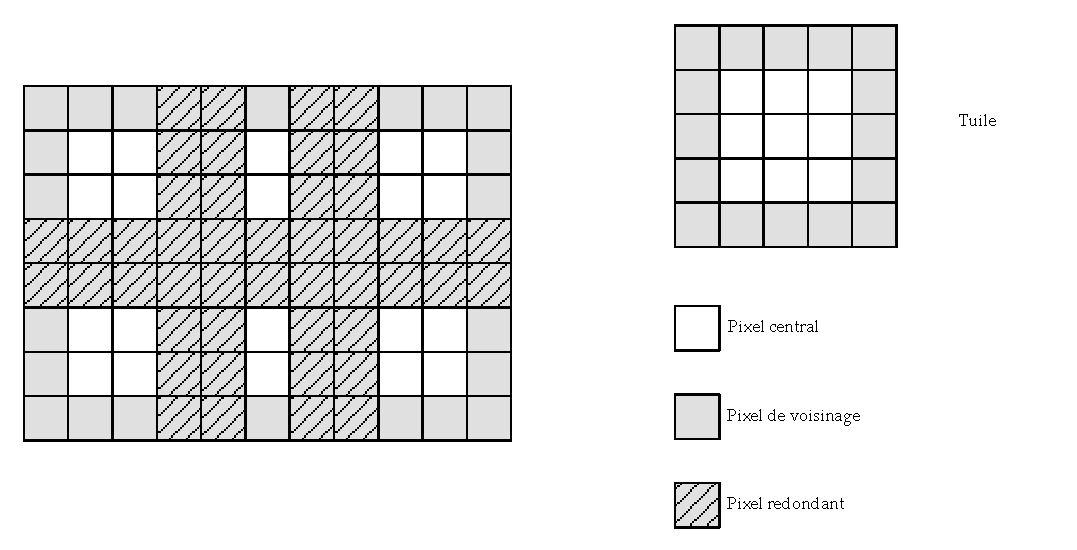
\includegraphics[width=\columnwidth]{Chapter3/figures/qreloads}
  \label{qreloads}
  \caption{Redondances de donn�es pour un op�rateur de convolution $3 \times 3$}
\end{figure}
Les tuile que l'on traite dans notre cas sont en g�n�ral d'une forme rectangulaire. Toutefois, � cause de la pr�sence d'op�rateurs de convolution, les dimensions hauteur et largeur de la tuile ($h$ et $w$) doivent �galement �tre consid�r�es. En effet, dans le cas d'op�rateurs de convolution les bords qui repr�sentent les voisinage des pixels trait�s augmentent la quantit� de donn�es transf�r�es de la m�moire. Cette quantit� peut �tre r�duite avec un choix judicieux des dimensions de la Tuile. Comme le montre la figure \ref{qreloads}certains des pixels sont recharg�s, nous d�montrons dans la suite l'influence des dimensions de la tuile sur ce nombre de pixels redondants.\\
\indent Si l'on consid�re une image de hauteur $H$ et de largeur de $W$, une tuile de dimensions $h$ et $w$ et un op�rateur de convolution n�cessitant un voisinage pour chaque pixel. On suppose pour simplifier le calcul, que la matrice de convolution est carr�e, ce qui fait que les bords des deux c�t�s sont �gaux. La quantit� totale de pixels transf�r�es pour le traitement est alors :
\begin{equation}
Q = (h+2b)\times(w+2b)\times nb_{tiles}\nonumber
\end{equation}
o� $nb_{tiles}$ est le nombres de tuiles dans l'image.
\begin{equation}
nb_{tiles} = \frac{H \times W}{h \times w} \nonumber
\end{equation}
Le but �tant de trouver � taille de tuile constante $h\times w$ quels sont les dimensions $h$ et $w$ qui minimisent $Q$
\begin{equation}
Q = (h+2b)\times(w+2b)\times\frac{H \times W}{h \times w} \nonumber
\end{equation}

Posons alors $\lambda = h \times w = C^{te}$, la fonction � minimiser devient alors :
\begin{equation}
Q = (h+2b)\times(w+2b)\times\frac{H \times W}{\lambda} \nonumber
\end{equation}
Calculons alors les d�riv�es  : \begin{equation}\frac{\partial Q}{\partial h} \mbox{ et } \frac{\partial Q}{\partial w} \nonumber\end{equation}

\begin{equation} Q = \frac{H \times W}{\lambda} (h+2b) \times (\frac{\lambda}{h}+2b) \mbox{  et sym�triquement  } Q = \frac{H \times W}{\lambda} (w+2b) \times (\frac{\lambda}{w}+2b) \nonumber\end{equation}

\begin{equation}
%$\frac{\partial Q}{\partial h} = \frac{H \times W \times 2b}{\lambda \times h^{2}}(h^{2}-\lambda)$
\frac{\partial Q}{\partial h} = \frac{H \times W \times 2b}{\lambda \times h^{2}}(h^{2}-\lambda) \nonumber \\
\end{equation}
\begin{equation}
\frac{\partial Q}{\partial w} = \frac{H \times W \times 2b}{\lambda \times w^{2}}(w^{2}-\lambda) \nonumber
\end{equation}
Le minimum de la fonction $Q$ est atteint lorsque : \begin{equation}\frac{\partial Q}{\partial h} = 0 \mbox{ et } \frac{\partial Q}{\partial w}  = 0\nonumber\end{equation}

ce qui donne \begin{equation}h = w = \sqrt{\lambda} \nonumber \end{equation}
\begin{figure}[htb]
  \centering
  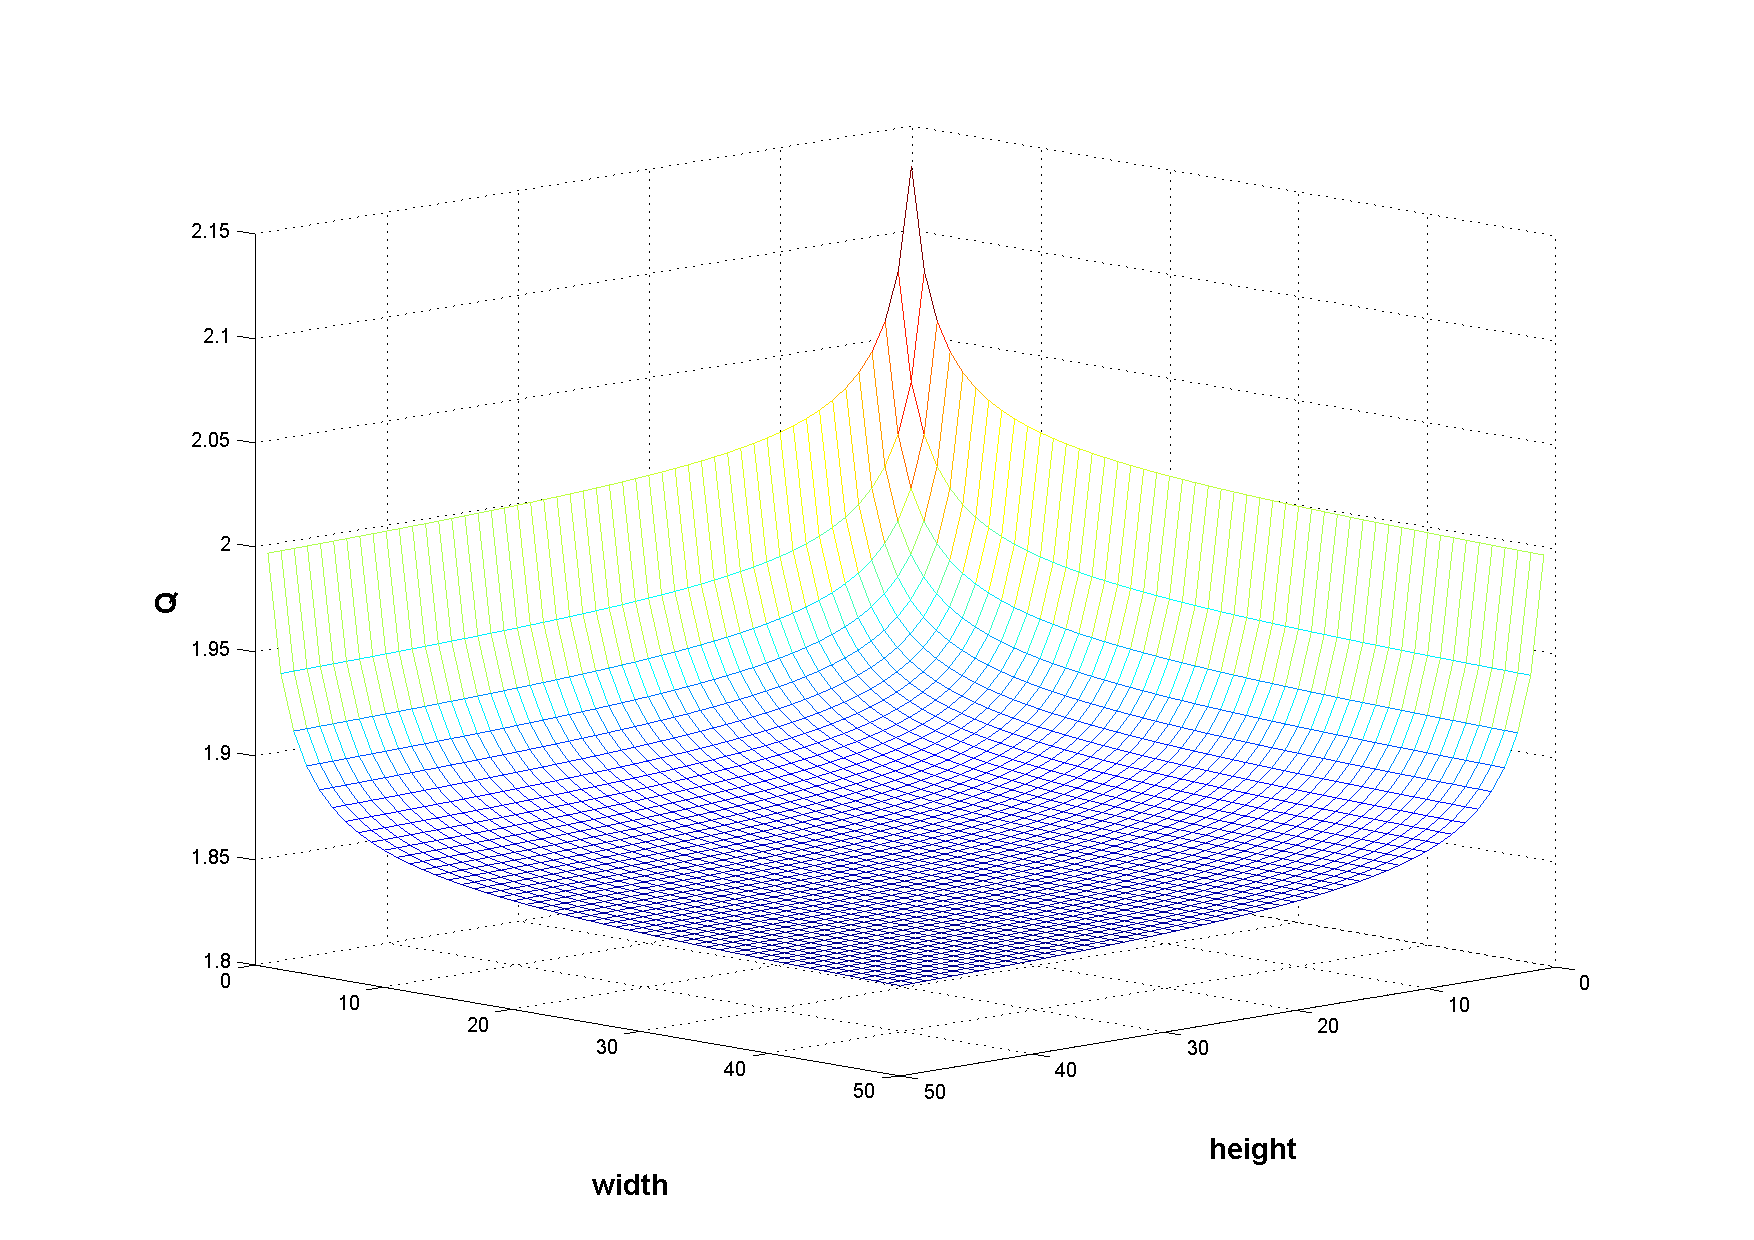
\includegraphics[width=\columnwidth]{Chapter3/figures/meshtile}
  \caption{Trac� de la fonction $Q(h,w)$ dans l'espace}
  \label{meshtile}\end{figure}
Ce qui permet de d�duire que la forme de la tuile qui minimise la quantit� de donn�es transf�r�e est une forme carr�e. D'autre par lorsque l'on observe le trac� de la fonction $Q$ sur la figure \ref{meshtile} on peut constater que cette fonction d�croit quand $h$ et $w$ augmentent et que la valeur de $Q$ est minimale pour une surface de tuile donn�e ($h \times w = C^{te}$) lorsque $h = w$ ce qui correspond � la premi�re bissectrice du plan $(hw)$. Ceci permet d'affirmer d'une part que la tuile carr�e est optimale pour une surface donn�e et que la valeur de $Q$ diminue d'autant plus lorsque $h$ et $w$ augmentent. Les valeurs de $h$ et $w$ sont alors limit�es par l'espace m�moire disponible pour une tuile dans la m�moire locale des SPEs.\\
\indent Ce r�sultat nous a permis de d�montrer que la forme de la tuile avait une influence sur la quantit� de donn�es transf�r�es et par cons�quent sur la performance globale de l'application. Cependant, ce d�coupage n'est pas forc�ment optimal lorsqu'on passe � l'impl�mentation. En effet, des tuiles de formes carr�es signifient des acc�s � des zones non-contigues de la m�moire. Ce type d'acc�s est en g�n�ral couteux car il provoque des sauts dans la m�moire. De plus, sur le processeur Cell, ceci se traduit en commandes DMA sur des zones non-contigues de la m�moire ce qui n�cessitent des commandes du type \emph{DMA list}. Ces derni�res requi�rent la cr�ation d'une liste qui contient chaque DMA �l�mentaire et qui est d'autant plus grande que le nombre de transferts est important. Cette liste doit �galement �tre mise � jour lors de chaque nouveau transfert. Toutes ces contraintes nous ont pouss� dans un premier temps � adopter un d�coupage en bandes qui consiste � ce que les tuiles aient une largeur �gale � celle de l'image. Ceci permet que les acc�s se fassent uniquement sur des zones contigues de la m�moire et que les transferts puissent se faire avec une seule commande DMA. De plus, lorsqu'une tuile ne contient pas de bords lat�raux comme dans notre cas, le probl�me d'alignement des transferts est �galement contourn�. Par contre, ce choix induit des limitations en terme de taille d'image pouvant �tre trait�e. En effet, sachant que la taille de la tuile est limit�e et que sa largeur est �gale celle de l'image, la hauteur de la tuile elle, diminue au fur et � mesure que la largeur de l'image augmente. De ce fait, les acc�s non-contigus sont n�cessaires pour des taille d'images tr�s grandes.
\subsection{Sch�mas de Parall�lisation}
Dans ce qui suit, nous abordons l'optimisation de notre algorithme � un niveau d'abstraction plus haut qui est celui des t�ches. L'architecture du Cell permet plusieurs placements possibles du graphe d'op�rateurs par la pr�sence de 8 SPEs et la possibilit� de mettre en place diff�rents sch�mas de communication. Dans les figures qui suivent les op�rateurs sont repr�sent�s par des cercles, les processeurs par des rectangles � coins arrondis, les tuiles sont de forme rectangulaire et peuvent contenir des bords. Les fl�ches � trait fin repr�sentent des instruction \texttt{LOAD/STORE} dans la m�moire priv�e du SPE alors que les fl�ches plus �paisses repr�sentent des commandes DMA inter-SPE ou alors entre la m�moire centrale et le \emph{local store} d'un SPE.
\subsubsection{SPMD Conventionnel}
\begin{figure}[!htb]
	\centering
  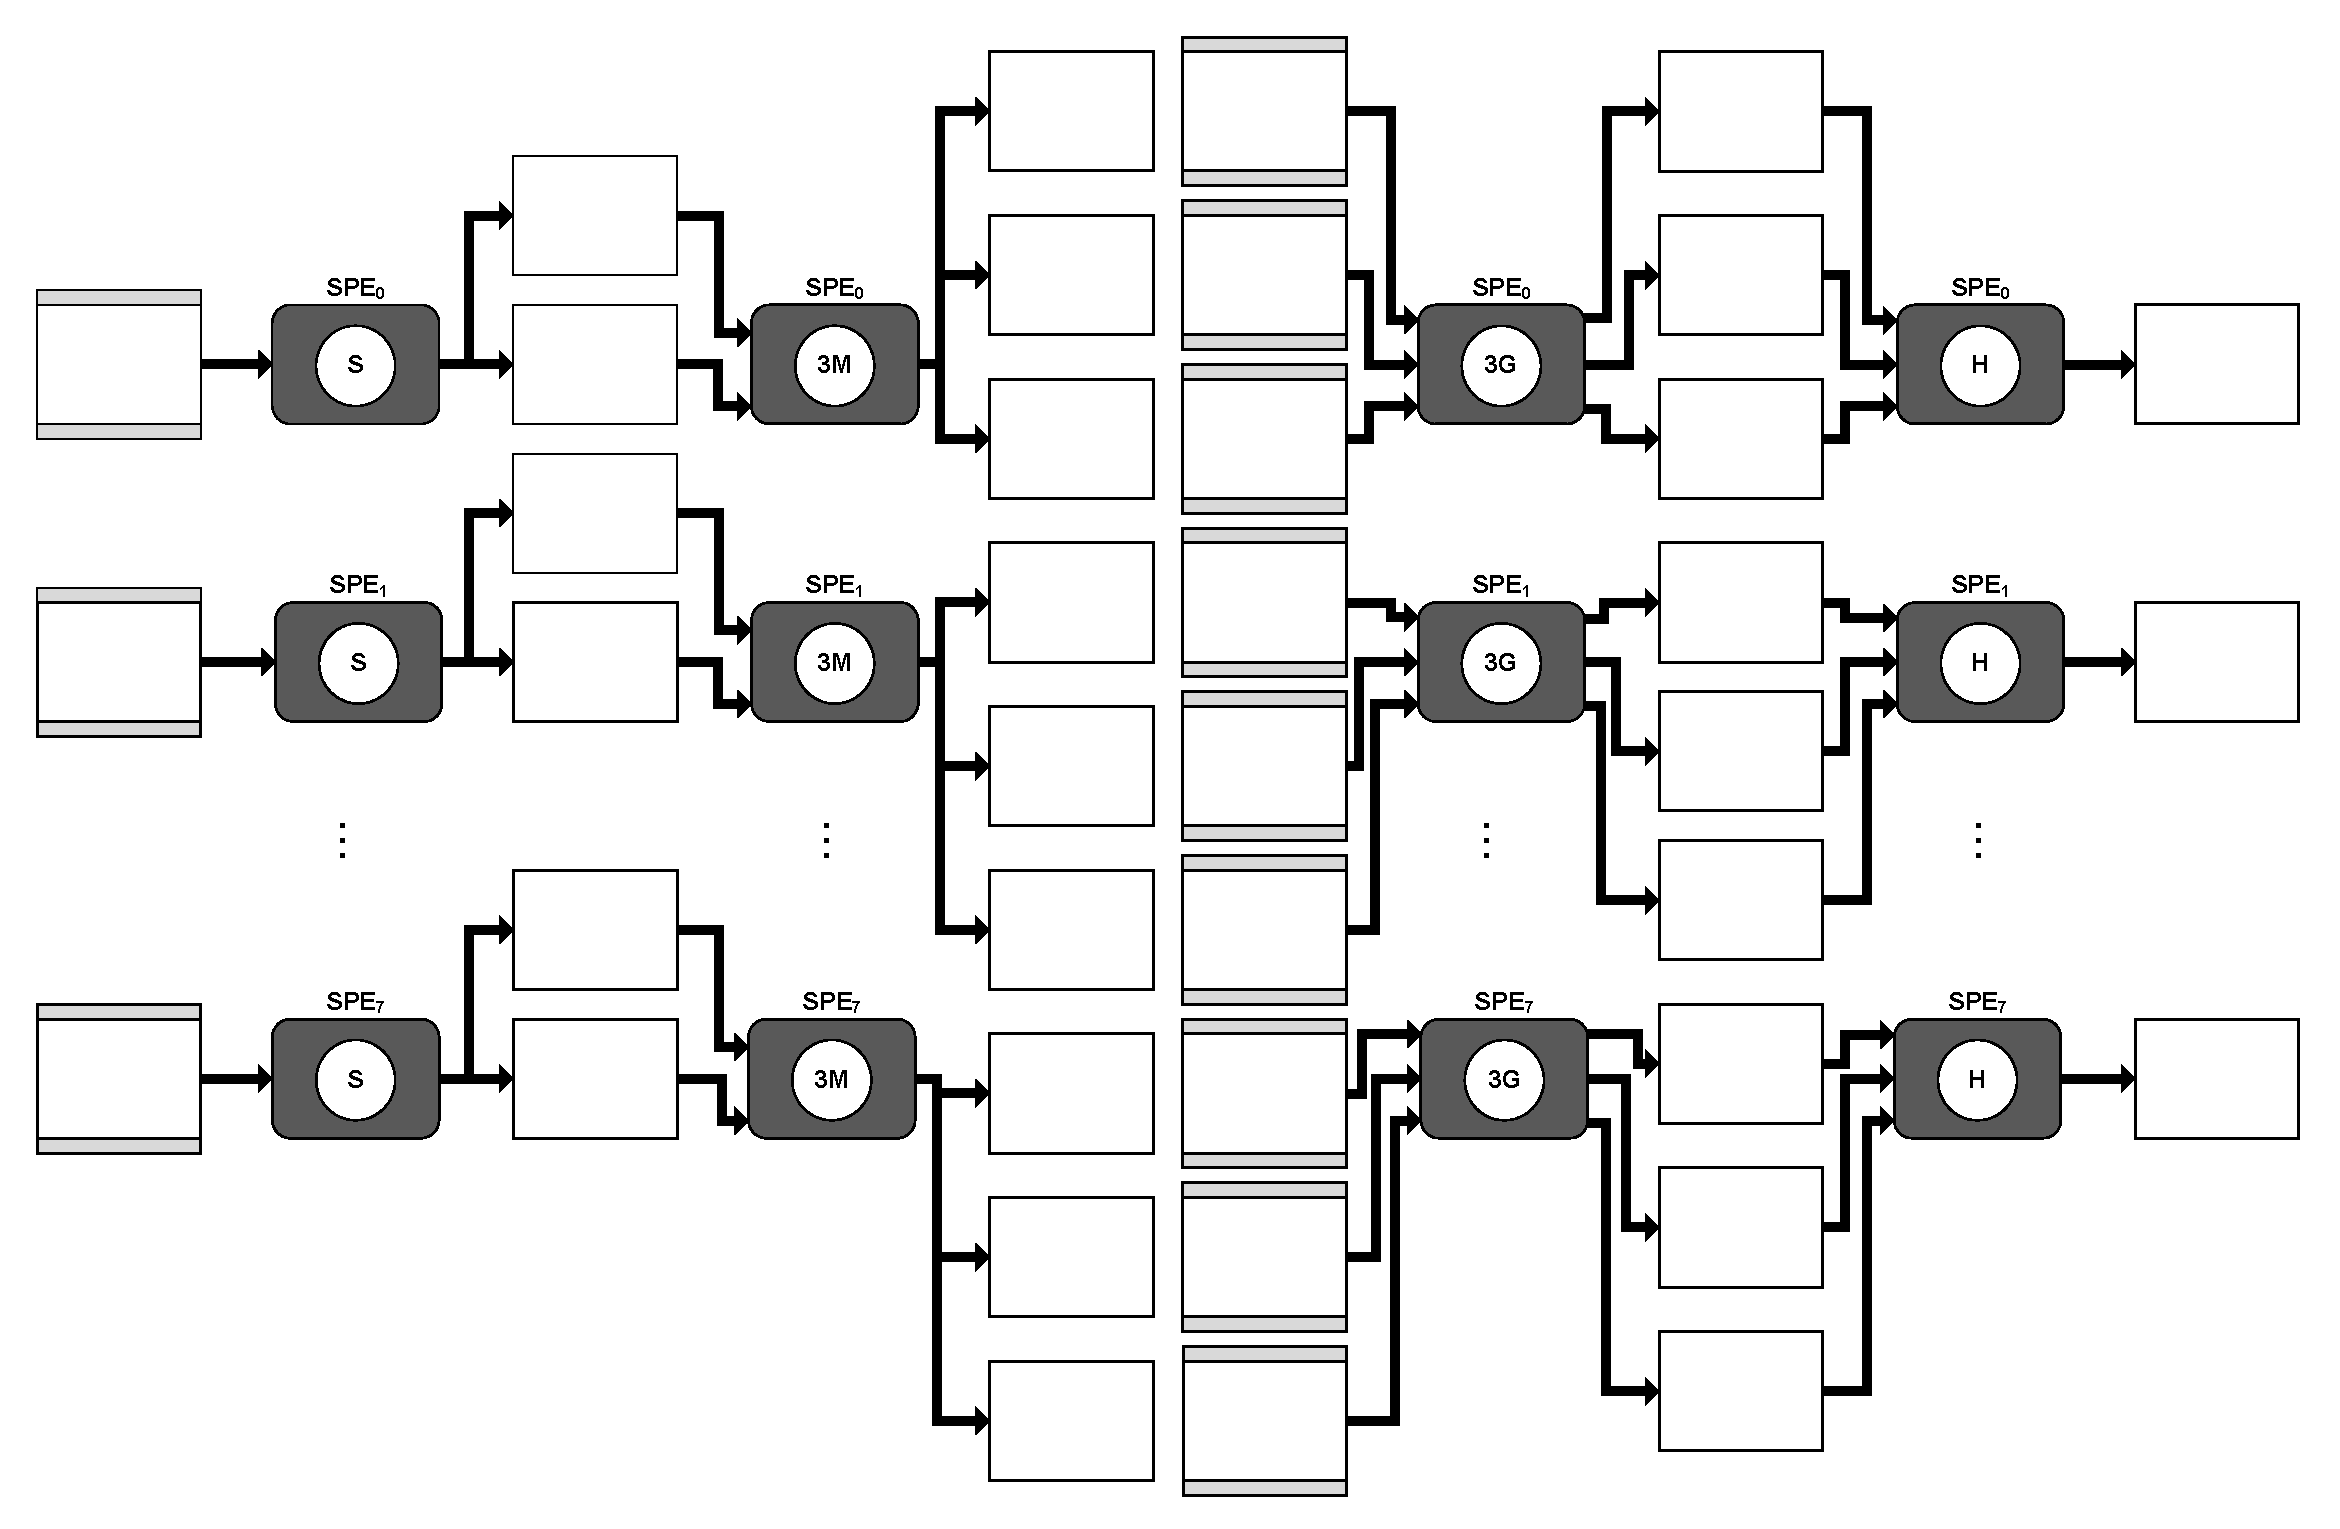
\includegraphics[width= \columnwidth]{Chapter3/figures/harris-spmd}
  \label{harris-spmd}
	\caption{Sch�ma de Parall�lisation SPMD Conventionnel}
\end{figure}
Dans ce sch�ma de d�ploiement, l'image est divis�e en 8 r�gions de m�me taille, afin que chacun des 8 SPEs ait une charge de calcul �quivalente. Tous les SPEs ex�cutent le m�me code. Les op�rateurs sont ex�cut�s successivement sur l'image enti�re l'un apr�s l'autre. A titre d'exemple l'op�rateur de multiplication n'est ex�cut� que lorsque le calcul du filtre de \emph{Sobel} est achev� sur toute l'image. Ce mod�le de calcul est dit \emph{data-parallel} car les donn�es sont envoy�es en parall�le sur les SPEs et trait�es de mani�re compl�tement ind�pendantes les unes des autres. Toutefois, la bande passante sur le bus m�moire centrale vers \emph{locale store} est beaucoup sollicit�e car les donn�es sont syst�matiquement lues et �crites avant et apr�s chaque op�rateur.
\subsubsection{Pipeline Conventionnel}
\begin{figure}[!htb]
	\centering
  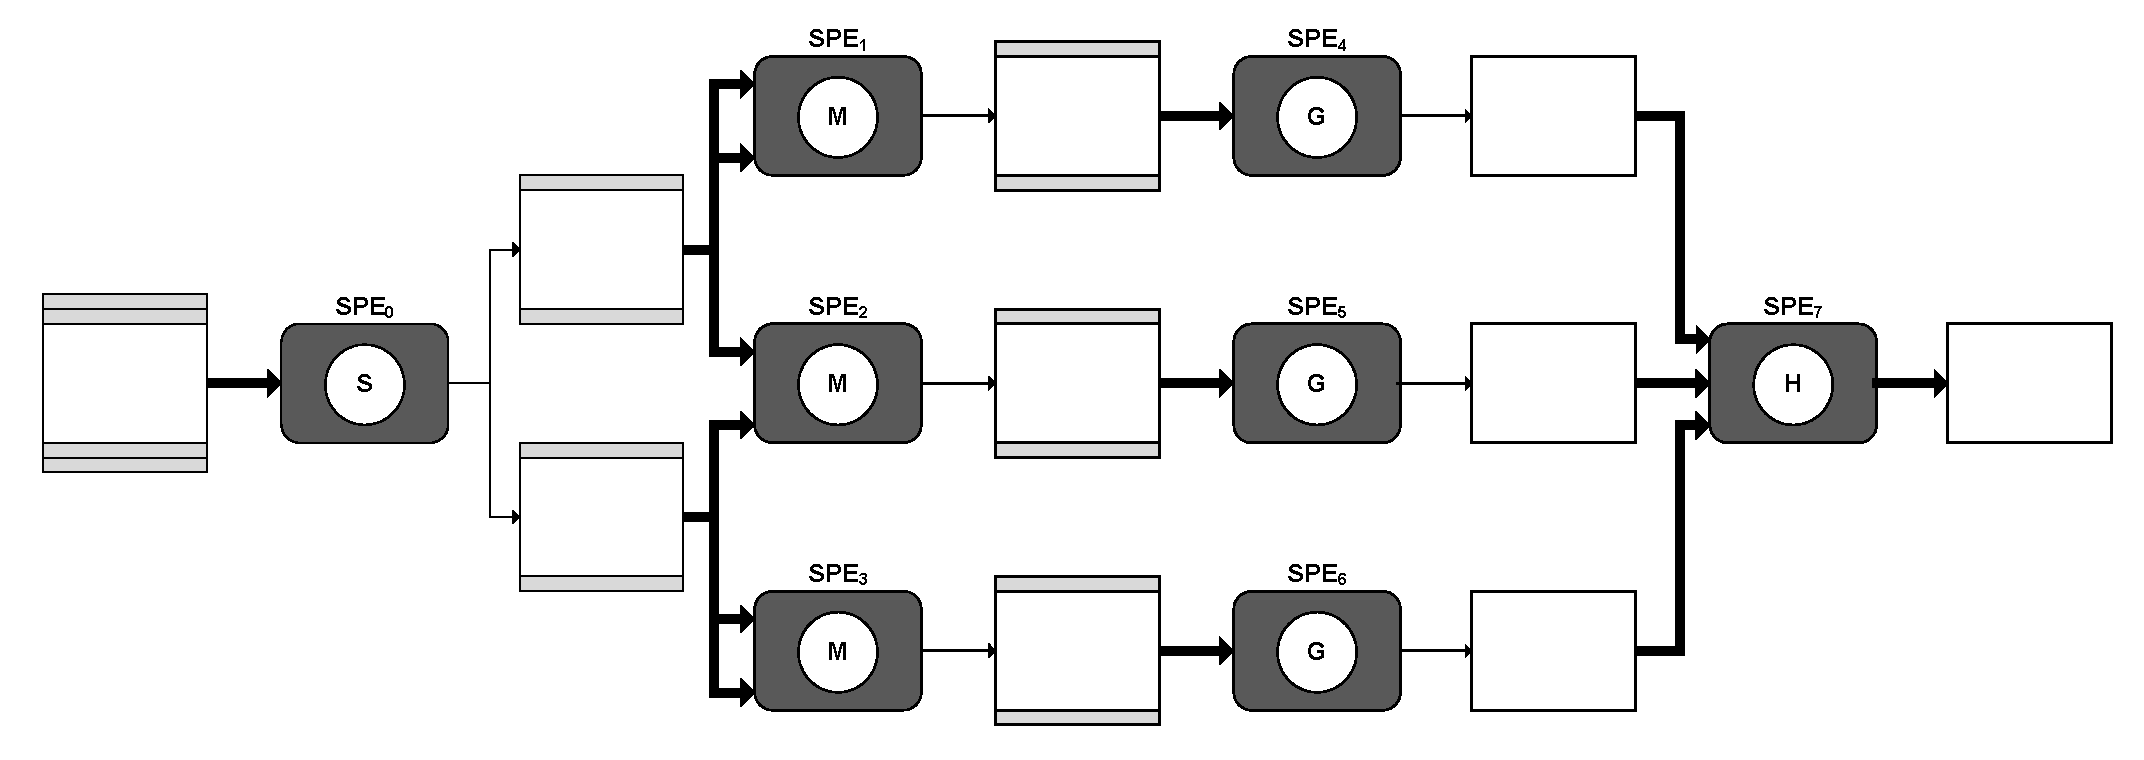
\includegraphics[width= \columnwidth]{Chapter3/figures/harris-pipeline}
	\caption{Sch�ma de Parall�lisation Pipeline}
	\label{harris-pipeline}
\end{figure}
Cette impl�mentation de l'algorithme consiste � d�ployer le graphe d'op�rateur sous forme de pipeline. L'image n'est pas subdivis�e en r�gions de traitement mais chaque tuile trait�e traverse le pipeline avant qu'une nouvelle tuile ne puisse le faire. L'algorithme est par cons�quent fortement s�quentialis�. Par contre la bande-passante inter-SPEs est bien exploit�e car la majorit� des transferts se font entre SPEs et par cons�quent la pression exerc�e sur le bus pr�c�demment est att�nu�e car elle est r�partie sur l'ensemble de l'anneau.
\subsubsection{Chainage d'op�rateur par paires}
\begin{figure}[!htb]
	\centering
  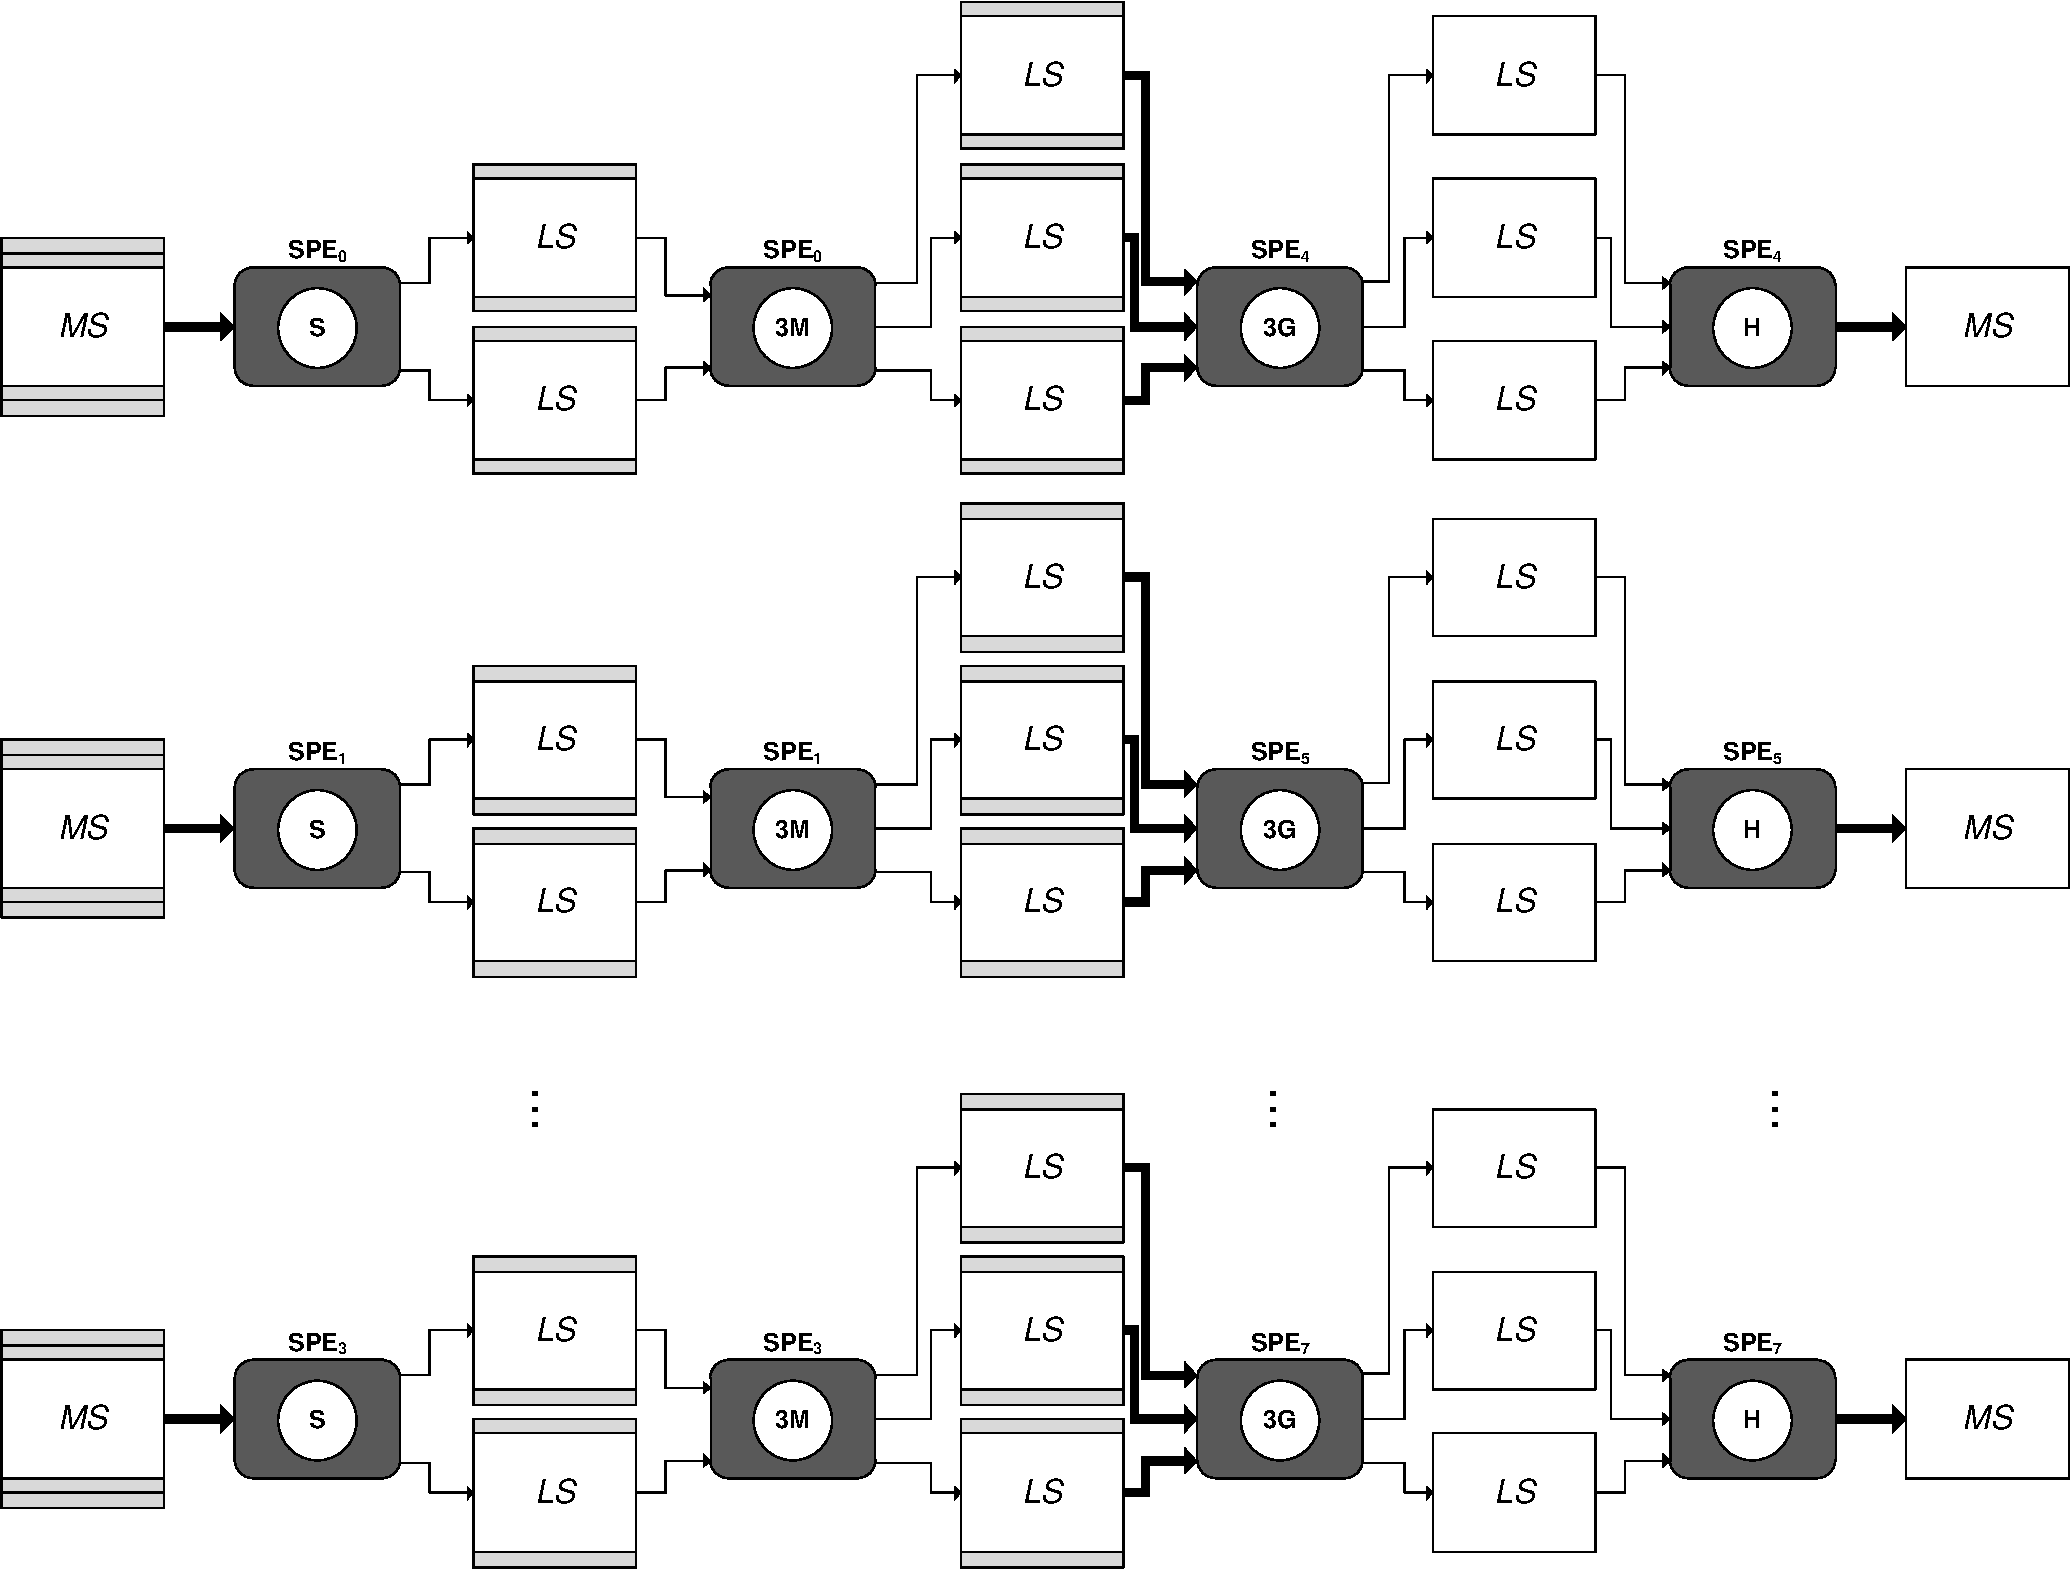
\includegraphics[width= \columnwidth]{Chapter3/figures/harris-hchain}
	\caption{Sch�ma de Parall�lisation Chainage d'op�rateurs par paires}
	\label{harris-pipeline}
\end{figure}
Dans cette version deux op�rateurs successifs sont plac�s sur le m�me SPE. Ainsi, les op�rateur \emph{Sobel} et \emph{Mul} sont plac�s sur un m�me SPE et \emph{Gauss} et \emph{Coarsity} sont plac�s sur un autre SPE. Le nombre de SPEs dans un processeur Cell �tant de 8, ce sch�ma permet d'avoir 4 r�gions de l'image trait�es en parall�le. Si l'on compare cette version � la pr�c�dente, on notera que la pression sur le bus d'interconnexion est plus importante car les transferts concurrents sont plus nombreux et par cons�quent le risque de contention du bus est plus probable.
\subsubsection{Chainage et fusion d'op�rateur par paires}
\begin{figure}[!htb]
	\centering
  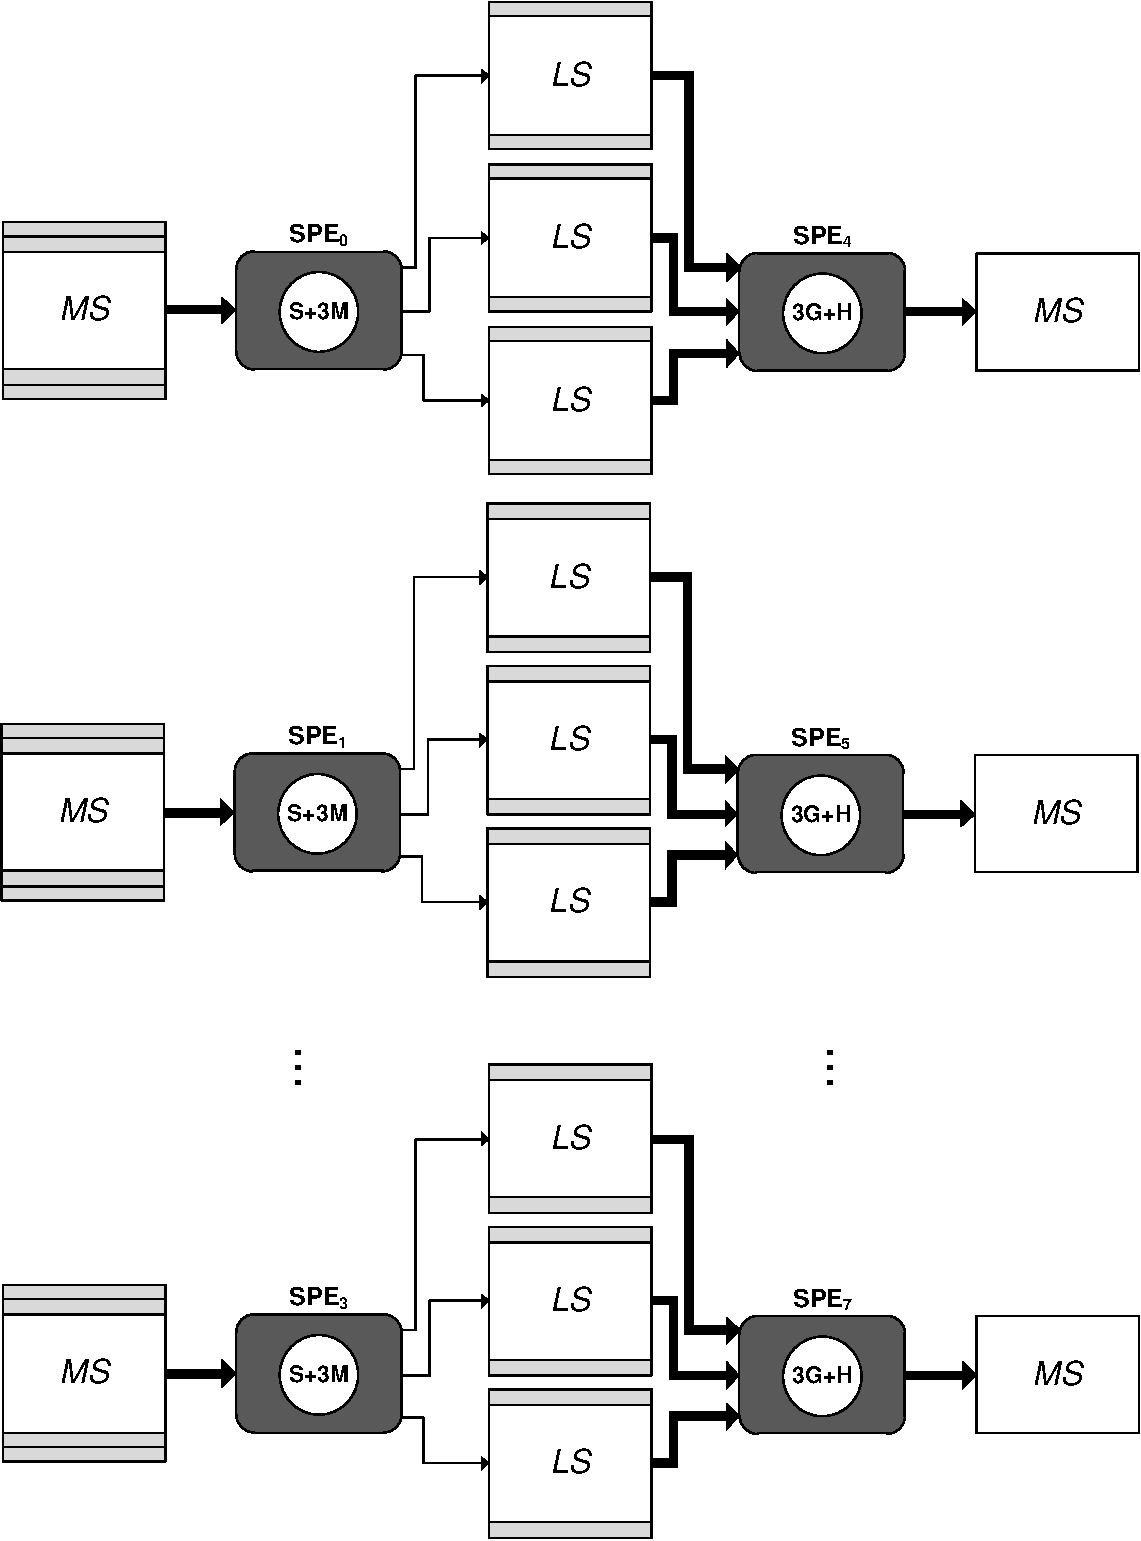
\includegraphics[width= 0.6\columnwidth]{Chapter3/figures/harris-hchainhpipe}
	\caption{Sch�ma de Parall�lisation Chainage et fusion d'op�rateurs par paires}
	\label{harris-pipeline}
\end{figure}
Cette version est une variante de celle qui la pr�c�de. L'id�e �tant de fusionner les op�rateurs pr�sents sur un m�me SPE, et ce afin d'�liminer les instructions de \texttt{LOAD} et \texttt{STORE} pr�sent � la sortie de du premier et � l'entr�e du second. De ce fait, le nombre de cycles peut �tre consid�rablement r�duit, surtout lorsque l'on sait que la latence des instructions m�moire est de 6 cycles sur les SPE \cite{cell_handbook}.
\subsubsection{Cha�nage entier et fusion d'op�rateur par paires}
\begin{figure}[htb]
	\centering
  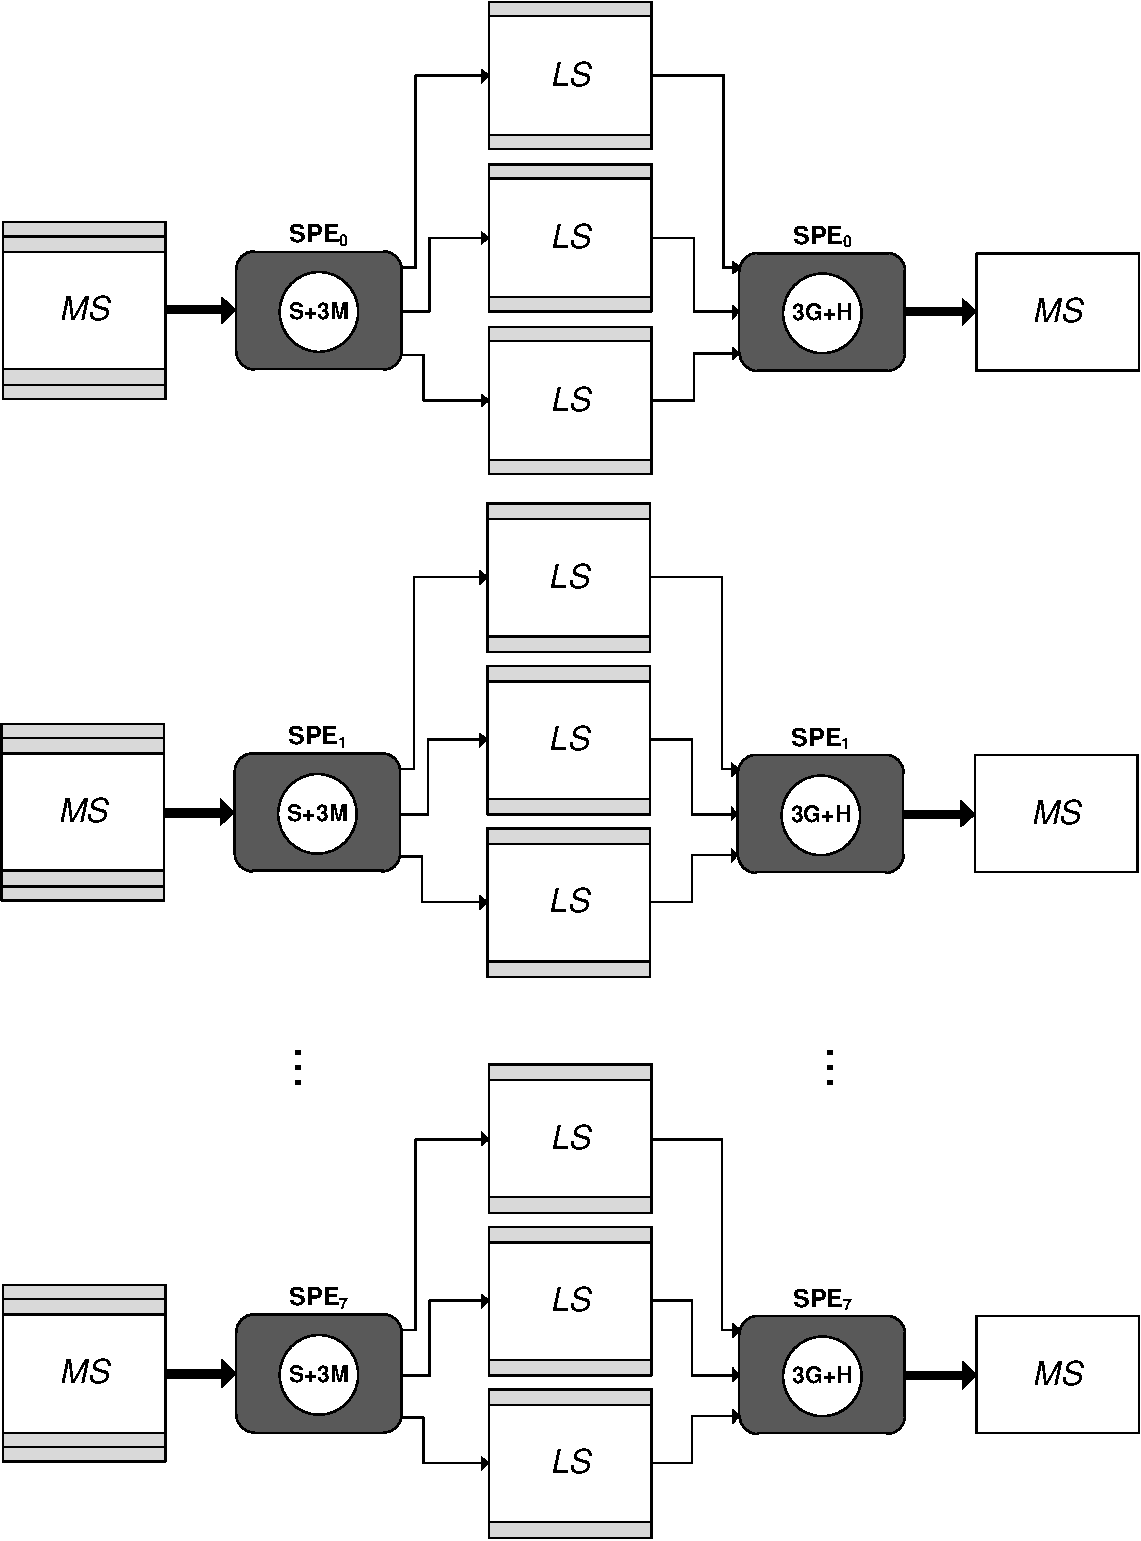
\includegraphics[width= 0.6\columnwidth]{Chapter3/figures/harris-hchainfpipe}
	\caption{Sch�ma de Parall�lisation Cha�nage et fusion d'op�rateurs par paires}
	\label{harris-pipeline}
\end{figure}
Dans cette impl�mentation tous les op�rateurs sont ex�cut�s sur le m�me SPE. D'une part ceci permet d'�viter les transferts DMA entre SPE et minimise donc les transactions sur le bus d'interconnexion.
\section{\'Evaluation des Performances}
apr�s avoir expos� les diff�rentes techniques d'optimisations nous proc�dons � la mesure de performance pour les diff�rents mod�les de d�ploiement pr�c�dents. Il s'agit ici de comparer les mod�les en terme de temps d'ex�cution sur le processeur Cell. Dans un deuxi�me temps nous �valuons l'influence des transferts sur la performance globale de chacun des mod�les.
\subsection{M�triques de Mesure}
La m�trique que nous avons choisi d'utiliser pour la mesure de performance, est le nombre de cycles moyen par pixel ou $cpp$, \begin{equation}cpp = \frac{nombre_{cyles \mbox{ } cpu}}{nombre_{pixels}} = \frac{nombre_{cyles \mbox{ } cpu}}{H \times W} \nonumber\end{equation}. Les bancs de tests ont �t� con�us de telle sorte � mesurer d'une part la performance brute ainsi que d'autres m�triques sp�cifiques aux architectures parall�les qui sont des m�triques de passage � l'�chelle (\emph{scalability}) notament l'acc�l�ration \emph{speedup} et l'efficacit� \emph{efficiency}.
\subsection{M�thode et Plateforme de Mesure}
La plate-forme sur laquelle a �t� men�e l'�valuation des performance est un Blade QS20 d'IBM cadenc� � 3.2 GHz. Cette lame contient deux processeurs Cell, chacun reli� � une m�moire de 512 MB, ce qui donne au total 1 GB de \emph{RAM} disponible. Le timer utilis� pour la mesure la performance est appel� \emph{timebase} et il est cadenc� � 14.318 $Mhz$. L'OS install� est un Linux, distribution Fedora 7. Le d�veloppement � �t� r�alis� sur le \emph{Cell SDK 3.0} et les compilateurs utilis�s sont \emph{ppu-gcc} et {spu-gcc}, ce qui implique une compilation du type \emph{dual-source} un pour le SPE et un pour le PPE.\\
\indent La m�thodologie de mesure adopt�e est en accord avec les syst�mes de vision par ordinateur. Nous avons simul� le cas d'un flux d'images continu, et avons mesur� le temps d'ex�cution moyen pour une image. Ceci permet de n�gliger l'\emph{overhead} induit par la cr�ation et la synchronisation des \emph{threads}. L'interface utilisateur permet de faire varier plusieurs param�tres, notamment la taille de l'image, la taille de la tuile et le nombre de SPEs.
\subsection{Comparaison des Sch�mas de Parall�lisation}
\begin{figure}[htb]
	\centering
  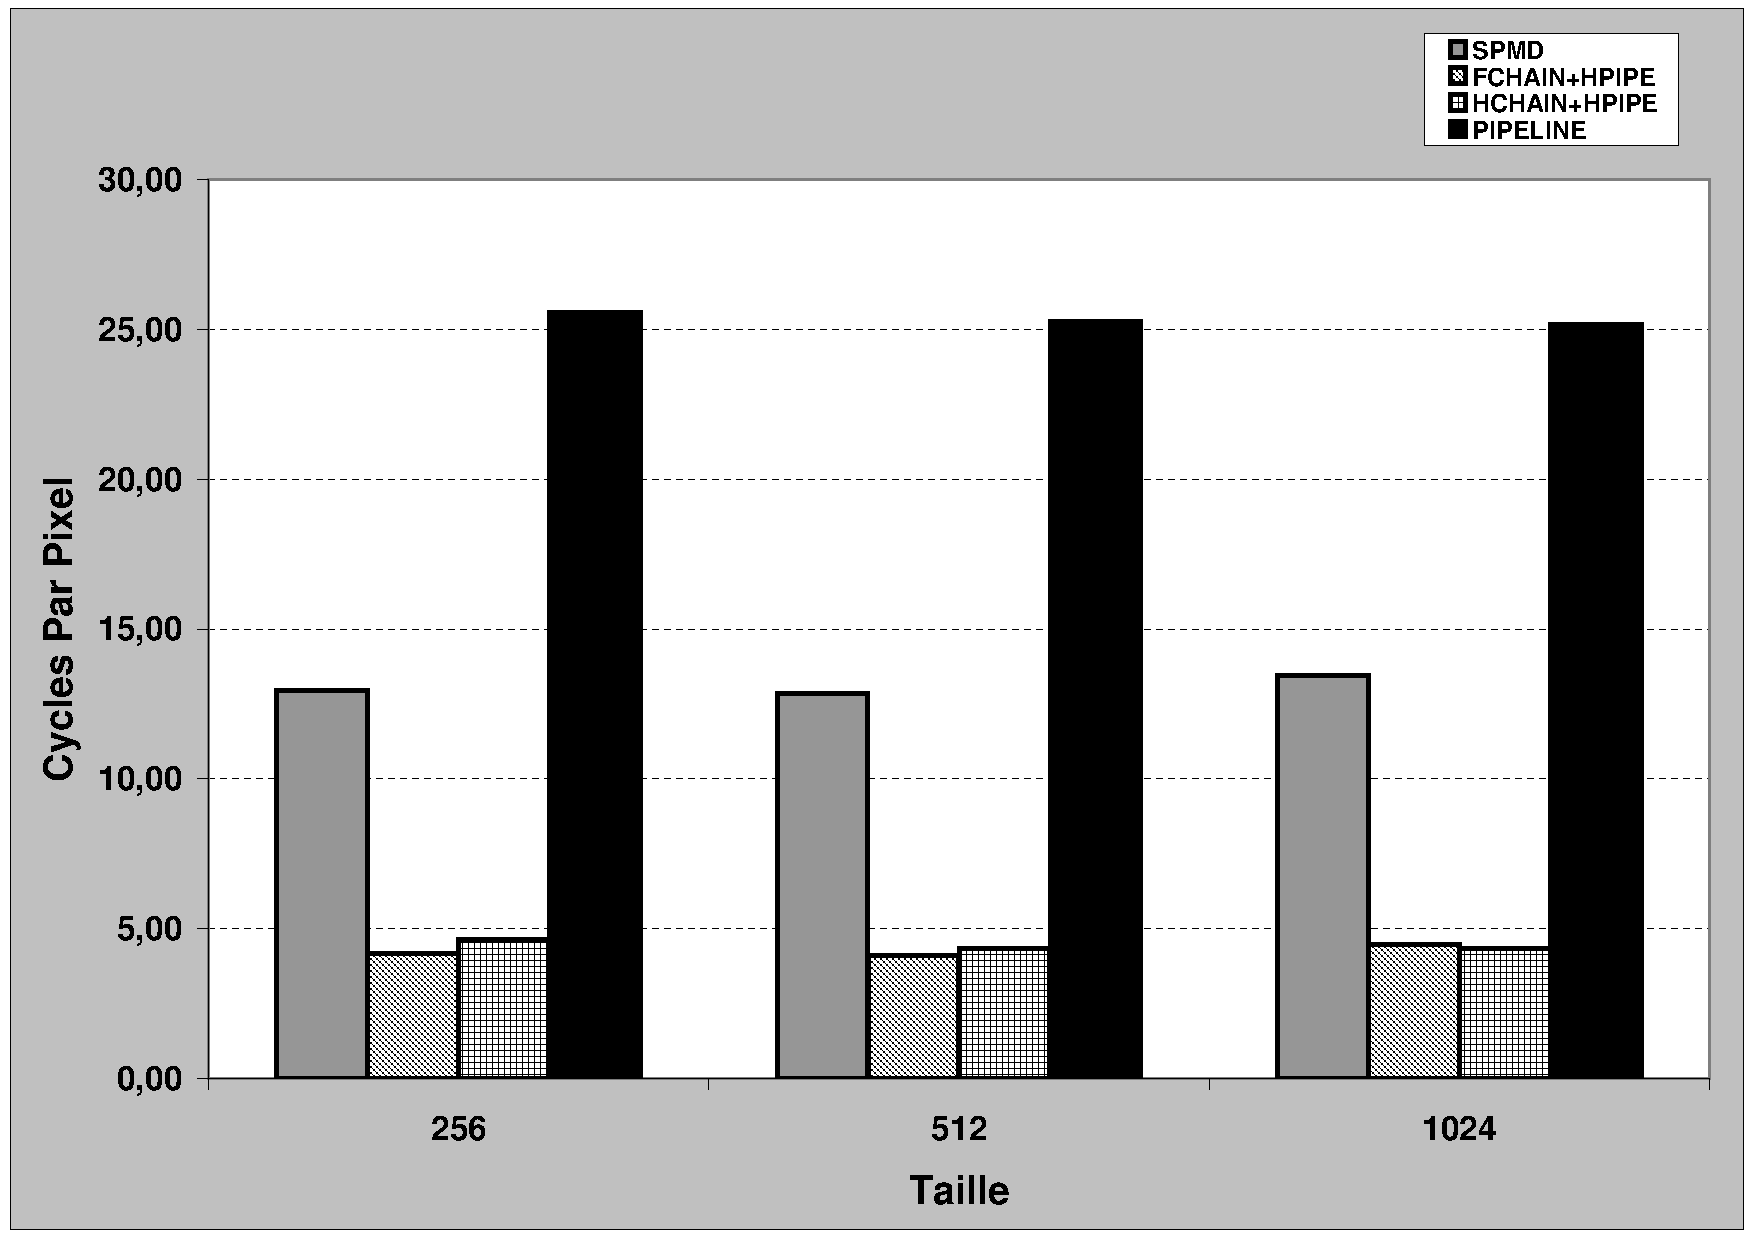
\includegraphics[width= 0.8\columnwidth]{Chapter3/figures/BenchCompareModels}
	\caption{Comparaison des mod�les en cycles par point}
	\label{comparemodels}
\end{figure}
La figure \ref{comparemodels} donne une comparaison entre les diff�rents mod�le de d�ploiement de l'algorithme de Harris sur le processeur Cell d�crits pr�c�demment. Ce que l'on peut observer en premier lieu c'est que le sch�ma \emph{pipeline} donne les plus mauvaises performances ce qui �tait attendu : cette versions est volontairement s�rialis�e et n'exploite pas enti�rement le parall�lisme de donn�es offert par l'architecture du Cell. Les autres r�sultats correspondent �galement � nos attentes : 
\begin{itemize}
\item Nos techniques d'optimisation des acc�s m�moires am�liorent sensiblement la performance globale car la version la plus rapide est celle ou les fonctions sont compos�es deux par deux  et ou tous les op�rateurs sont ex�cut�s sur le m�me SPE (remplacement des DMA par des \texttt{LOAD/STORE} ).
\item Les versions ou les DMA inter-SPE sont utilis�s poss�dent de bonnes performance : � titre d'exemple la versions sans composition de fonction et en regroupant deux op�rateurs par SPE est plus rapide que la versions SPMD.
\item De plus, la version avec composition de fonction ou les paires d'op�rateurs sont sur deux SPEs diff�rents est presque aussi rapide que la m�me versions ou tous les op�rateurs sont plac�s sur le m�me SPE. Ceci prouve que la bande-passante inter-SPE est comparable � celle des instructions \texttt{LOAD/STORE} sur les m�moires locales.
\end{itemize}
Dans ce qui pr�c�de nous avons pu constater que le placement optimal d'un graphe de fonctions sur le processeur Cell n'�tait pas forc�ment �vident lorsqu'il s'agit d'un algorithme de traitement d'image comme dans notre cas. D'une part, l'on a vu que le choix d'un sch�ma compl�tement \emph{data parallel} n'�tait pas forc�ment optimal, et qu'un sch�ma mixte avec une partie \emph{pipeline} imbriqu�� dans un sch�ma \emph{data parallel} donnait un r�sultat aussi bon qu'un sch�ma bas� purement sur le parall�lisme de donn�es. Ceci est en grande partie possible, gr�ce � un niveau suppl�mentaire de parall�lisme au niveaux de transferts. En effet, en favorisant les communications inter-SPE on profite pleinement de la bande passante du bus interne (204.8 GB/s) qui peut g�rer jusqu'� 12 transferts en parall�le alors que dans un sch�ma de transferts o� plusieurs SPEs communiquent avec la m�moire centrale les commandes sont forc�ment s�rialis�es et dans ce cas l� la bande passante est limit�e � 25.6 GB/s. 
\subsection{Influence de la Taille de la Tuile}
\begin{figure}[htb]
	\centering
  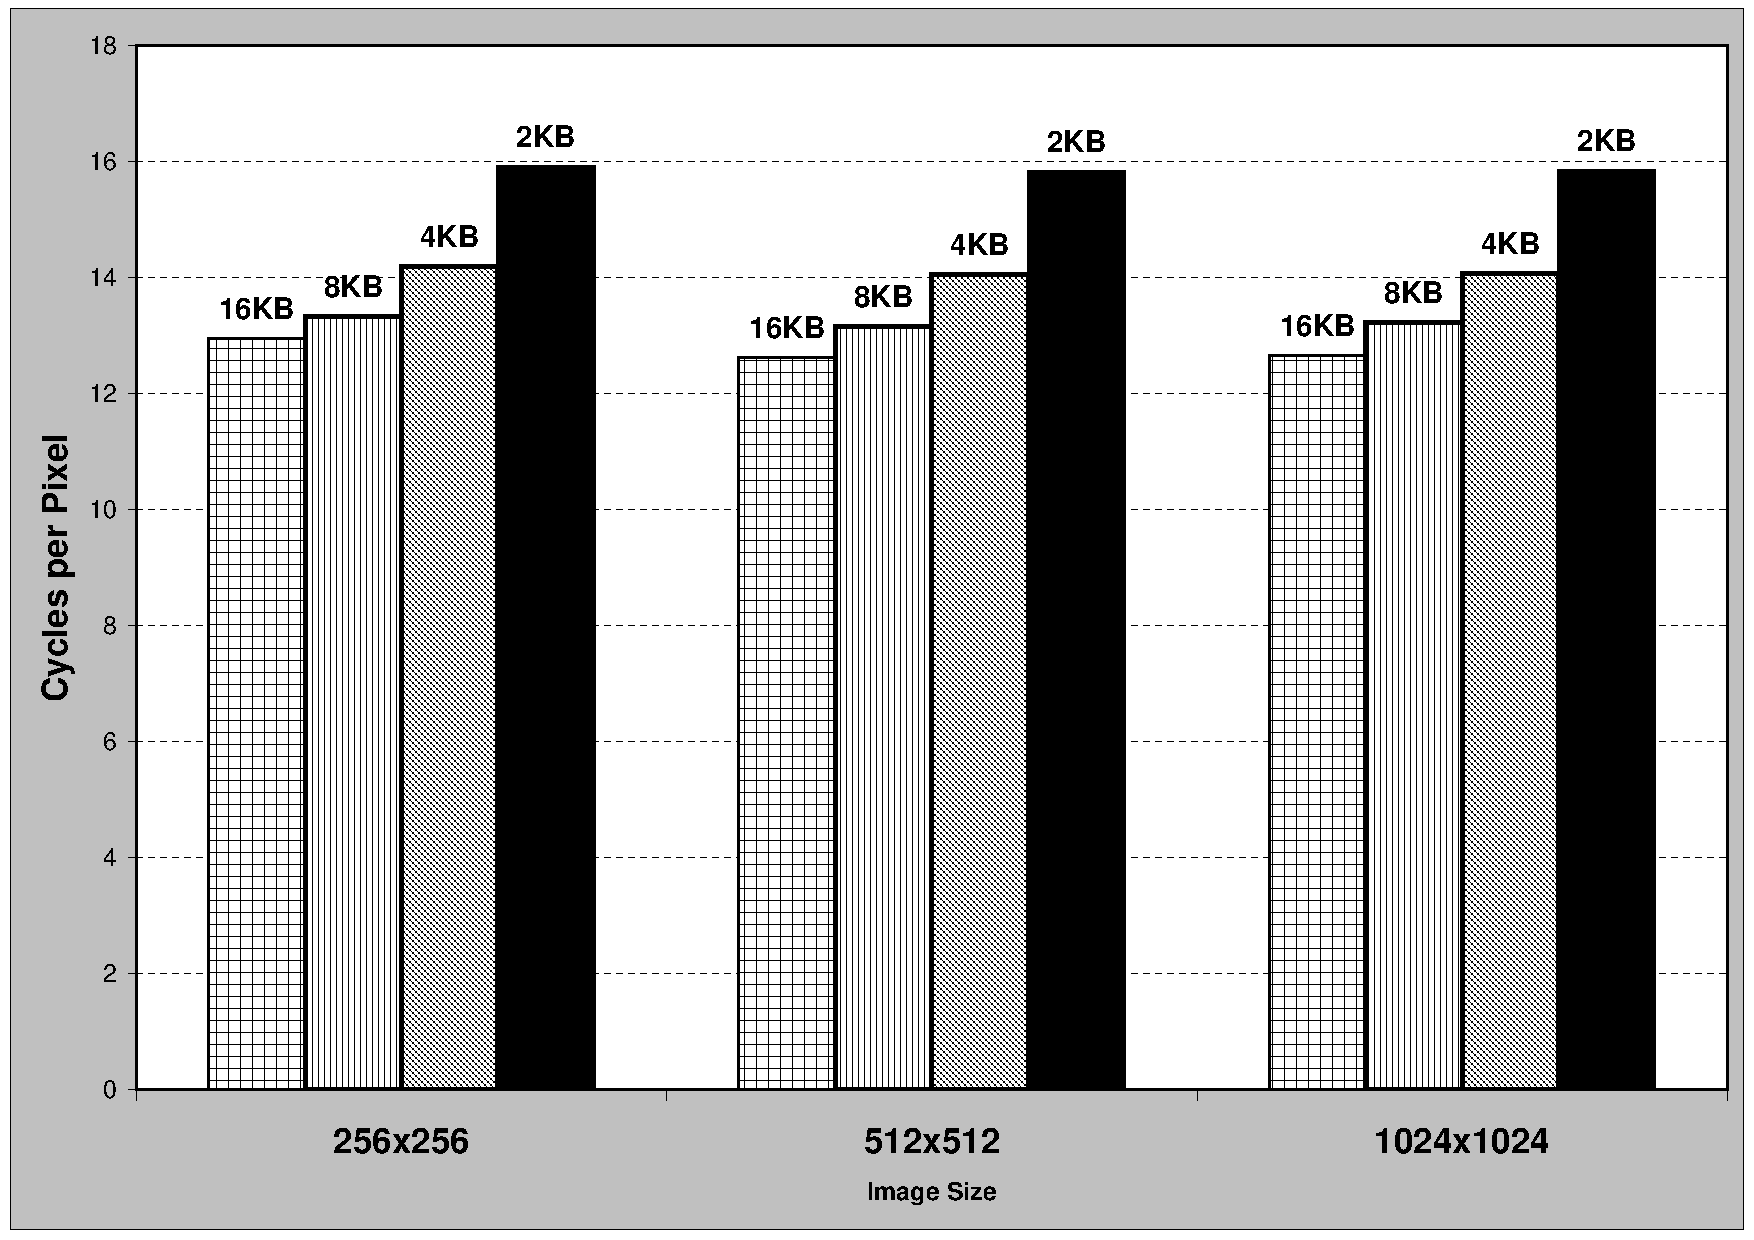
\includegraphics[width= \columnwidth]{Chapter3/figures/SizeTile}
	\caption{Influence de la taille de la tuile sur la performance pour la version chainage entier et fusion d'op�rateur par paires 1 SPU}
	\label{tilesize}
\end{figure}
Comme il est d�montr� dans \cite{cell_bw02} et \cite{cellnoc} la taille du bloc de donn�es transf�r� poss�de une influence sur la bande-passante du bus interne. Dans notre domaine d'application, la bande-passante m�moire est critique pour la performance globale de l'application, car les algorithmes de traitement d'image sont g�n�ralement caract�ris�s par un ratio transfert/calcul important. La figure \ref{tilesize} nous montre que la taille de tuile donnant les meilleures performance est 16KB, et ceci pour deux raisons:
\begin{itemize}
\item Une taille de bloc de 16 KB ou multiple de cette taille, garantit une bande-passante maximale sur le bus interne.
\item Comme nous l'avons vu dans la discussion sur la forme de la tuile, il est d�montr� que plus la taille de tuile est grande moins il y a de pixels redondants, et la quantit� de donn�es totale transf�r�es est minimis�e en ce qui concerne les noyaux de convolution.
\end{itemize}
\subsection{Analyse des R�sultats}
\begin{table}
\begin{tabular}{|c||c|c|c|}
\hline
\textbf{Mod�le} & \textbf{Op�rateur} & \textbf{Nombre de Cycles} & \textbf{Speedup} \\
\hline
\hline
\textbf{Halfchain} & Sobel+Mul+\texttt{LOAD/STORE}&119346&x \\
\hline
\textbf{Halfchain+Halfpipe} & Gauss+Coarsity+\texttt{LOAD/STORE}&188630&x \\
\hline
\textbf{Halfchain} & (Sobel $\circ$ Mul)+\texttt{LOAD/STORE}&16539& 7.2 \\
\hline
\textbf{Halfchain+Halfpipe} &(Gauss $\circ$ Coarsity)+\texttt{LOAD/STORE}&504309& 3.5 \\
\hline
\end{tabular}
\caption{Apport de la composition de fonction � la performance}
\label{tabspuperf}
\end{table}

La comparaison de la performance globale des diff�rents sch�mas d'impl�mentation ne suffit pas � prouver que l'optimisation de l'utilisation de la m�moire sont les facteurs principaux de l'am�lioration de la performance. Dans le but de donner une analyse plus pr�cise et donc plus compl�te, nous avons effectu� des mesures au niveau du SPE ou nous avons estim� le gain apport� par la composition des fonctions et les transferts DMA inter-SPE. Le tableau \ref{tabspuperf} donne en nombre de cycles \emph{SPU} les versions ou les op�rateurs ne sont pas compos�s deux � deux et celle ou elles le sont. Comme on peut le constater, cette optimisation permet d'avoir une acc�l�ration pouvant atteindre $\times 7.2$. Cette techniques, permet une utilisation maximale des registres au d�triment de la m�moire et par cons�quent elle est limit�e par la taille du banc de registres du processeur (128 registres pour le SPU. D'autre part l'optimisation de la localit� des donn�es en chainant les op�rateurs d'un m�me SPE est certe b�n�fique, mais elle est limit�e par le niveau de hi�rarchie m�moire juste au dessus des registres qui est le \emph{local store}, limit� lui � 256 KB.
\subsection{Mesure des M�triques de Passage � l'\'Echelle}

\begin{figure}[htb]
	\centering
  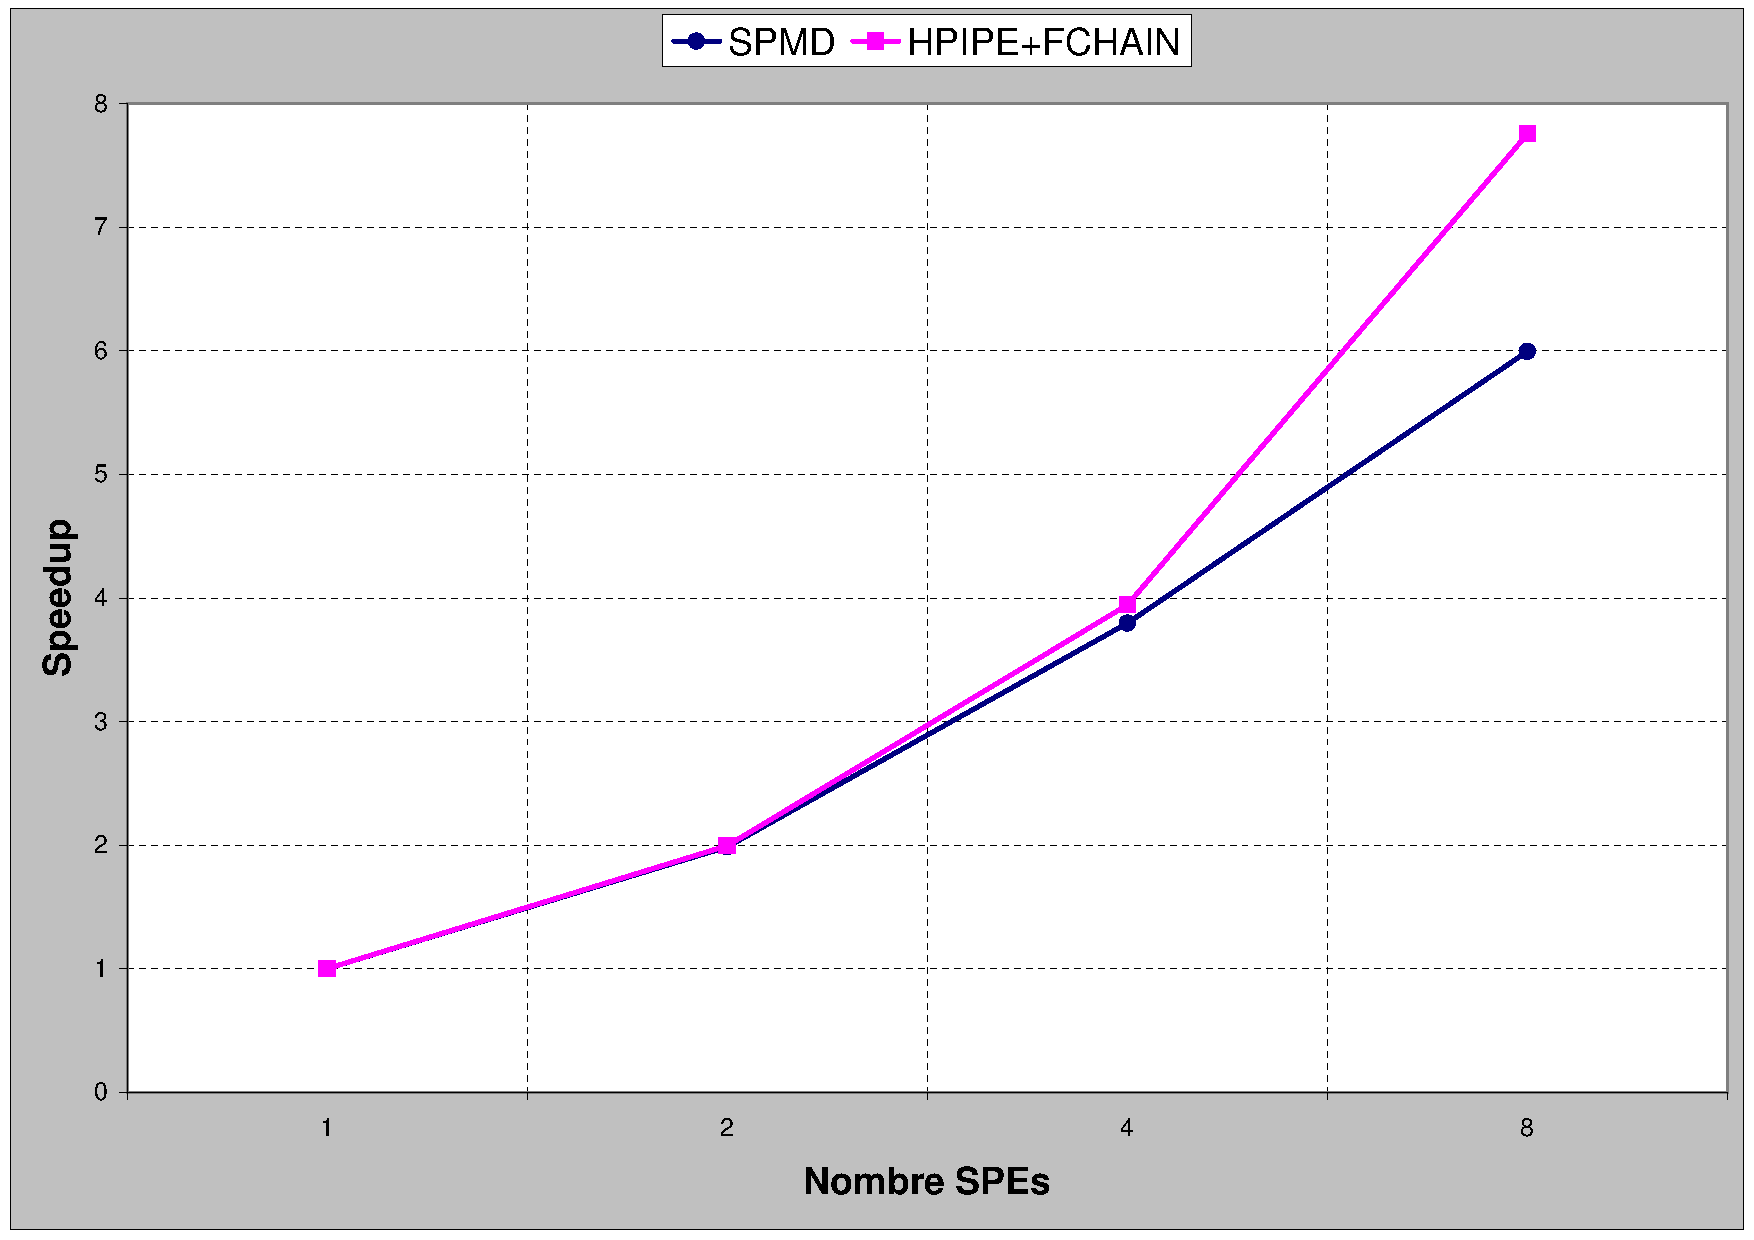
\includegraphics[width= 0.8\columnwidth]{Chapter3/figures/Speedup}
	\caption{Mesure du \emph{Speedup} en fonction du nombre de SPEs}
	\label{speedup}
\end{figure}

\begin{figure}[htb]
	\centering
 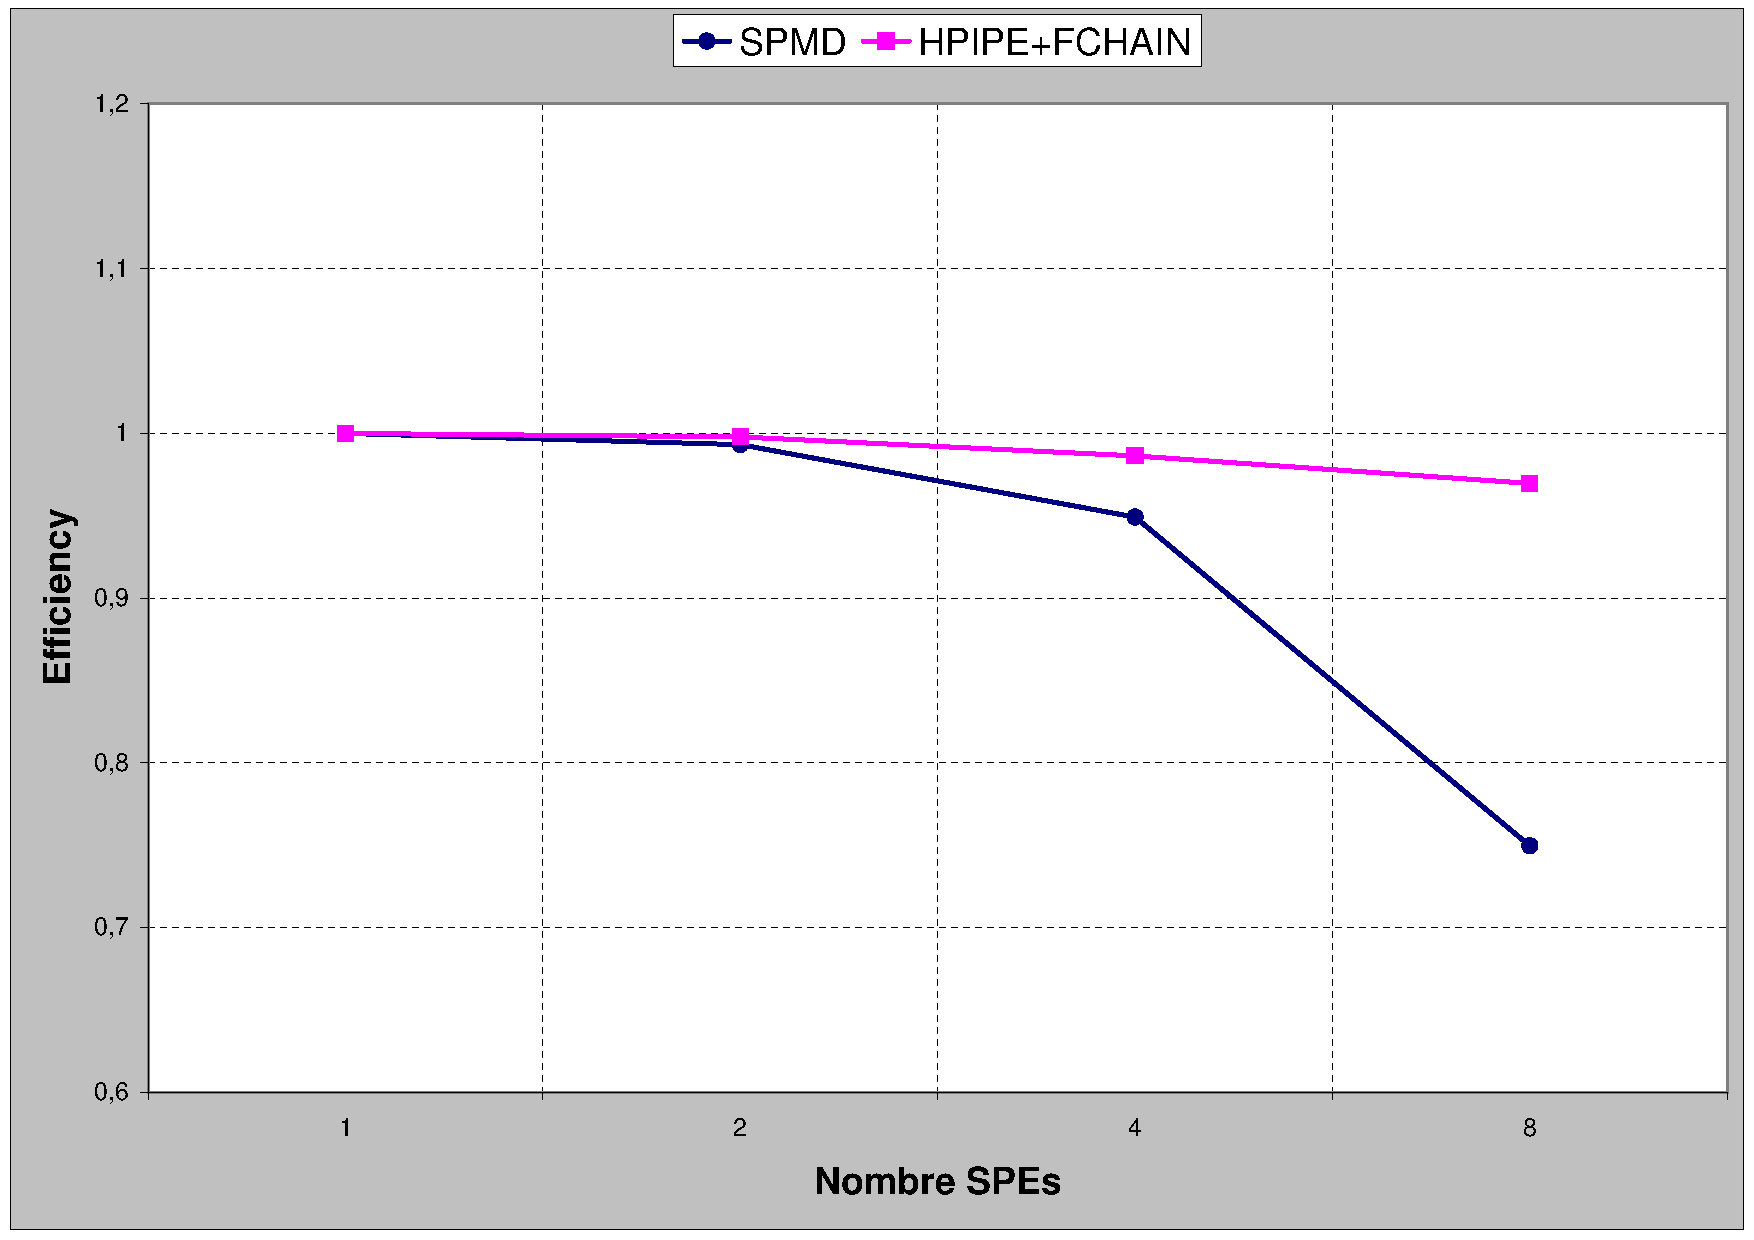
\includegraphics[width= 0.8\columnwidth]{Chapter3/figures/Efficiency}
	\caption{Mesure de l'Efficacit� en fonction du nombre de SPEs}
	\label{efficiency}
\end{figure}

Lorsque l'on mesure les performance d'une machine parall�le on ne peut se contenter de mesurer les performances temporelles brutes. Il est �galement int�ressant de s'attarder sur d'autres param�tres qui permettent de comparer deux architectures parall�les ou alors d'isoler un goulot d'�tranglement qui limite la performance. Ce que l'on veut �valuer est le passage � l'�chelle ou \emph{scalability} qui permet de mesurer sur un syst�me � plusieurs processeurs, le rendement des $N$ unit�s par rapport � un seul. Les m�triques les plus connues sont l'acc�l�ration (\emph{Speedup}) et l'efficacit� (\emph{Efficiency}), et sont d�finies comme suit:
\begin{equation}
Speedup = \frac{\mbox{Temps d'Ex�cution sur 1 Processeur}}{\mbox{Temps d'Ex�cution sur $P$ Processeur}} \nonumber
\end{equation}
\begin{equation}
Efficiency = \frac{\mbox{Temps d'Ex�cution sur 1 Processeur}}{P \times \mbox{Temps d'Ex�cution sur $P$ Processeur}}\nonumber
\end{equation}
Ces mesures sont essentielles pour l'adaptation d'un code s�quentiel � une machine parall�le. Elles permettent d'une part de d�tecter des limitations d'un syst�me parall�le pour la parall�lisation d'un code. Par exemple, on peut �valuer la complexit� due au contr�le des \emph{threads} et � leur synchronisation. D'autre part, on peut mesurer l'efficacit� du r�seau d'interconnection � distribuer les donn�es de mani�re parall�le au diff�rents noeuds. Elles peuvent �galement justifier l'ajout d'une quantit� suppl�mentaires de processeurs si cela n'alt�re pas la performance en induisant un co�t de gestion suppl�mentaire. \\
\indent D'apr�s les figures \ref{speedup} et \ref{efficiency} on peut constater que le Cell est une architecture ayant une bonne "scalabilit�". En effet, on peut noter dans les deux cas �tudi�s � la fois, un \emph{speedup} proche de $P$ le nombre de SPEs et une efficacit� proche de 1. On peut tout de m�me noter certaines diff�rences entre les deux impl�mentations �tudi�es, d'une part la version SPMD et d'autre part la versions avec composition de fonctions et chainage sur le m�me SPE. La premi�re implique une pression importante sur le bus de donn�es car presque tous les lectures/�critures m�moire se font sur la m�moire externe. Au contraire, la seconde minimise le trafic vers la m�moire externe. Ceci explique, la diff�rence au niveau de l'efficacit� et permet de d�duire que plus le ratio transfert/calcul est grand est moins le passage � l'�chelle est bon.
%\chapter{Squelettes Algorithmiques pour le Cell}
%La programmation parall�le structur�e qu'on appelle programmation par squelettes algorithmiques \cite{skeletons_cole} restraint l'expression du parall�lisme � la composition d'un nombre pr�d�fini de \emph{patterns} nomm�s squelettes. Les squelettes algorithmiques sont des briques de base g�n�riques, portables et r�utilisables pour lesquelles une impl�mentation parall�le peut exister. Ils sont issues des langages de programmation fonctionnelle. Un syst�me de programmation bas� sur les squelettes fournit un ensemble fixe et relativement limit� de squelettes. Chaque squelette repr�sente une mani�re unique d'exploiter le parall�lisme dans une organisation sp�cifique du calcul, tels que le parall�lisme de donn�es, de t�ches, le \emph{divide-and-conquer} parall�le ou encore le pipeline. En combinant ces \emph{patterns} le d�veloppeur peut construire une sp�cification haut-niveau de son programme parall�le. Le syst�me peut ainsi exploiter cette sp�cification pour la transformation de code, l'exploitant efficace des ressources ou encore le placement.\\
La composition des squelettes peut se faire d'une mani�re non-hi�rarchique en mettant en s�quence les diff�rents blocs en en utilisant des variables temporaires pour sauvegarder les r�sultats interm�diaires, ou alors de mani�re hi�rarchique en imbriquant les fonctions squelette et ce en construisant une fonction compos�e dans laquelle le code de plusieurs squelettes est pass� en param�tre d'un autre squelette. Ceci pr�sente une mani�re �l�gante d'exprimer le parall�lisme multi-niveau.\\
Dans un environnement de programmation declarative, comme dans les langages fonctionnels ou alors dans la programmation par squelettes, la composition hi�rarchique procure au g�n�rateur de code plus de libert� de choix pour les transformations automatiques et l'utilisation efficace des ressources, comme par exemple le nombre de processeurs utilis� en parall�le dans un niveau particulier de la hi�rarchie. les squelettes ne pouvant pas �tre imbriqu�s  sont g�n�ralement impl�ment�es avec juste une librairie g�n�rique alors que les squelettes nich�s requi�rent un pr�-traitement qui d�roule la hi�rarchie du squelette en utilisant par exemple les templates C++ ou les macros de preprocesseur en C.

\section{Mod�le de Programmation}
\begin{figure}[!htb]
	\centering
  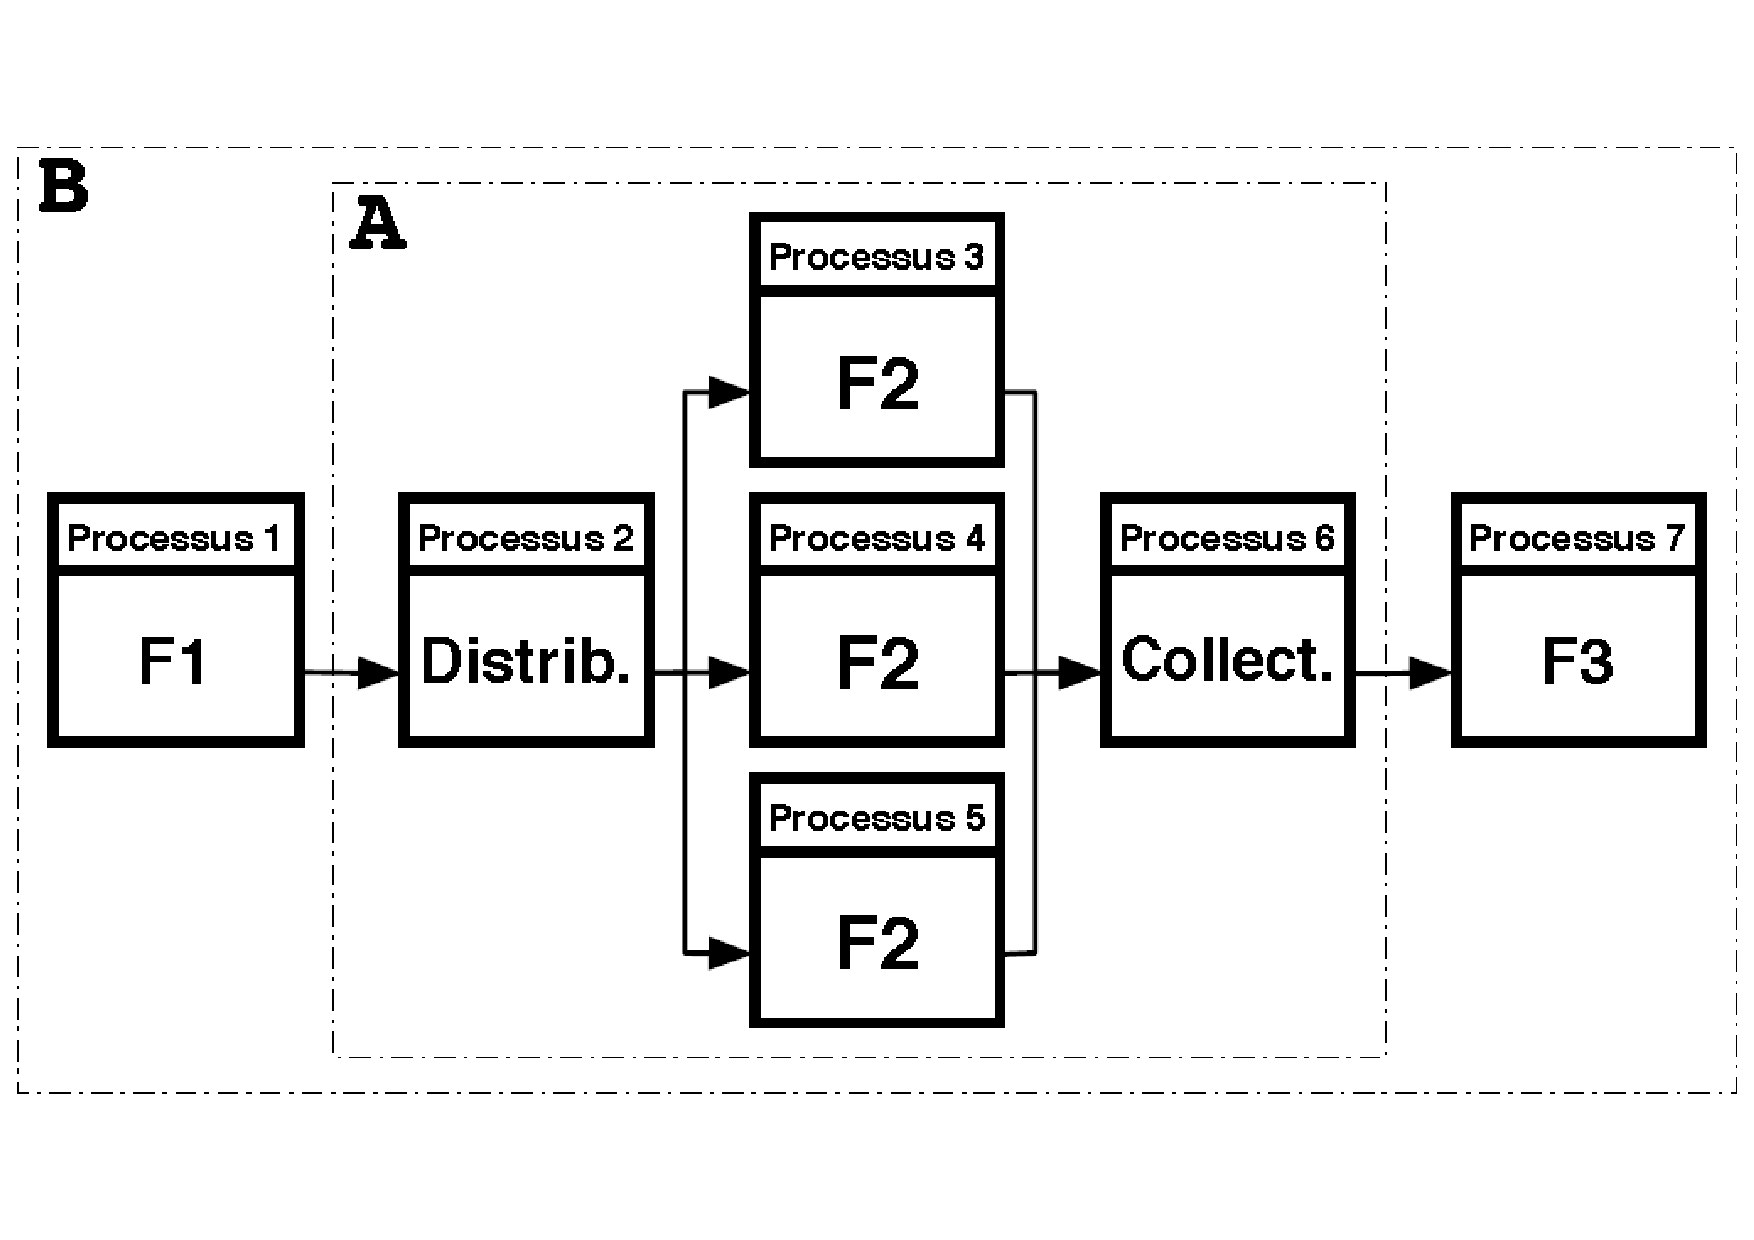
\includegraphics[width= 0.8\columnwidth]{Chapter3/figures/skeleton_example}
	\caption{Exemple de graphe de processus communicants avec hi�rarchisation}
	\label{skelexple}
\end{figure}
Dans le mod�le de programmation parall�le par squelettes algorithmiques, une application est d�finie comme �tant un graphe de processus communicants. Cette repr�sentation permet de sp�cifier les sch�mas de communication entre les processus \textbf{$P_{i}$}, de mettre en �vidence les fonctions s�quentielles \textbf{$F_{i}$} contenues dans l'application, ainsi que les processus n�cessaires � l'ex�cution parall�le de l'application. Un exemple de repr�sentation est donn� dans la figure \ref{skelexple}. On peut distinguer sur cette figure deux parties distinctes : 
\begin{itemize}
\item Le syst�me d'�quilibrage de charge \textbf{(A)} qui utilise $k$ processeurs qui traite les donn�es fournies par le processus \emph{Distrib}, ces derni�res �tant regroup�es par le processus \emph{Collect}. Il faudra noter que le flux alimente le processeurs de mani�re dynamique d�s qu'il trouve un processus libre.
\item Le m�canisme de contr�le \textbf{(A)} qui permet de s�quencer les traitement dans l'ordre donn�e par le graphe. Ce m�canisme assure que les donn�es, une fois trait�es (fonction $F_{i}$) par le processeur $P_{i}$, sont transmises au processus $P_{i+1}$. On pourra noter que le sch�ma d'ex�cution dans ce cas l� est du type \emph{pipeline}.
\end{itemize}
Le mod�le de programmation parall�le par squelettes algorithmiques repose sur l'extraction de tels sch�mas r�currents. Un squelette est ainsi d�fini comme �tant un sch�ma g�n�rique param�tr� par une liste de fonctions qu'il est possible d'instancier et de composer. Fonctionnellement, les squelettes algorithmiques sont des \textbf{fonctions d'ordre sup�rieur}, c'est � dire des fonctions prenant une ou plusieurs fonctions comme arguments et retournant une fonction comme r�sultat. La programmation par squelettes devient permet au programmeur d'utiliser un mod�le haut-niveau pour d�crire son application, sans se soucier de certains d�tails complexes comme l'ordonnancement ou le placement. Il peut alors d�finir une application parall�le comme suit:
\begin{itemize}
\item Instancier des squelettes en sp�cifiant les fonctions qui les d�finissent.
\item Exprimer la composition des ces squelettes.
\end{itemize}
L�expression de la compositions peut se faire en encodant cette derni�re sous la forme d�un \textbf{arbre}(\ref{fig_tree}) dont les noeuds repr�sentent les squelettes utilis�s et les feuilles, les fonctions s�quentielles pass�es en param�tres � ces squelettes.
\begin{figure}[!htb]
	\centering
  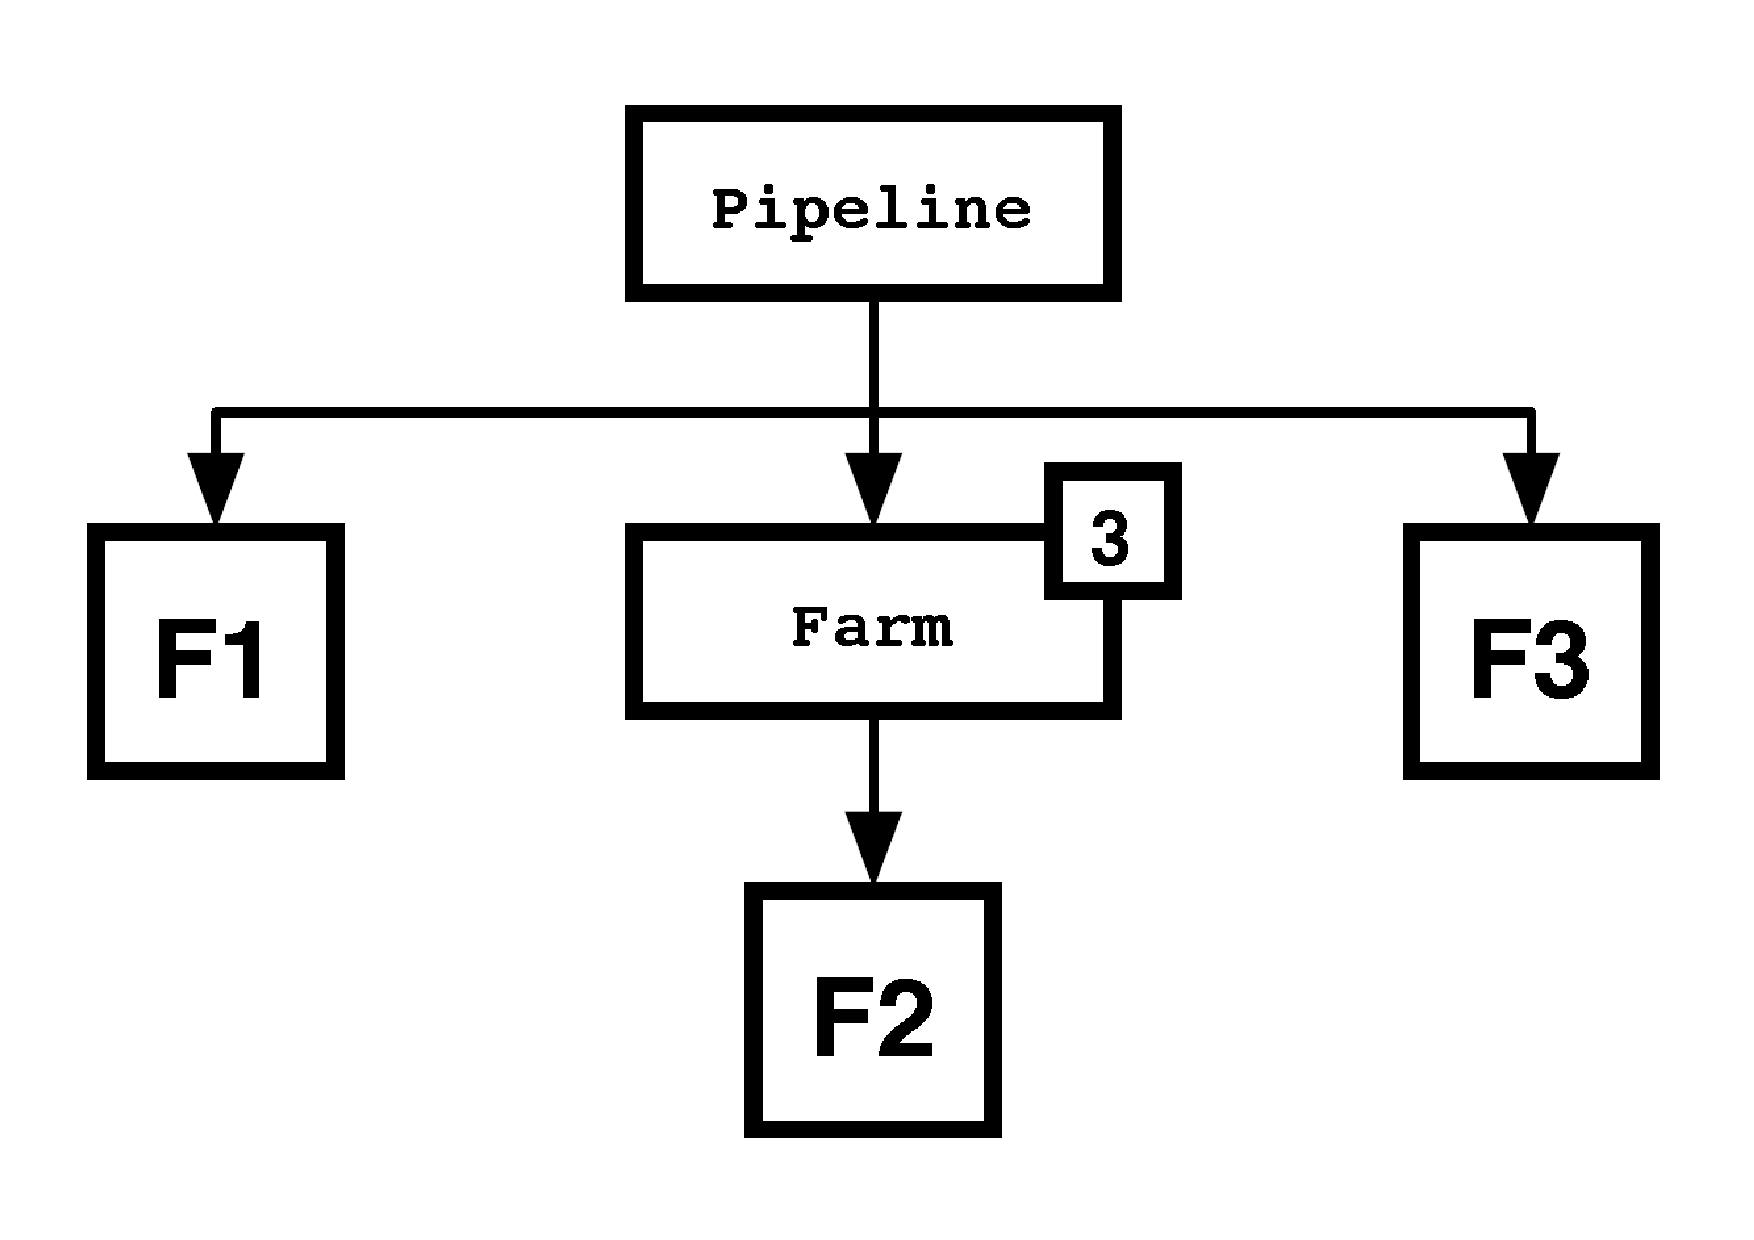
\includegraphics[width= 0.7\columnwidth]{Chapter3/figures/fig_tree}
	\caption{Arbre repr�sentant le squelette en Figure \ref{skelexple}}
	\label{fig_tree}
\end{figure}

Dans la figure \ref{fig_tree}, le squelette \textbf{Pipeline} d�crit le sch�ma g�n�rique correspondant � la section \textbf{B} du graphe de processus communiquant initial. Le squelette \textbf{Farm} repr�sente quant � lui la partie \textbf{A} de ce m�me sch�ma. Les fonctions $F_{i}$ apparaissent aux feuilles de l'arbre, c'est � dire en argument des squelettes. On note aussi que les fonctions \textbf{Distrib} et Collect n'apparaissent plus explicitement, car elles font partie int�grante du squelette \textbf{Farm}. Cette repr�sentation met en avant un des aspects les plus importants de l'approche
� base de squelettes algorithmiques : � partir d'un nombre restreint de squelettes (classiquement moins d'une dizaine), il est possible de d�finir des applications complexes. Ceci suppose toutefois que l'on ait formalis� le type d'application que l'on va chercher � parall�liser, de d�finir pr�cis�ment le jeu de squelettes que l'on d�sire mettre � disposition du d�veloppeur et de sp�cifier leurs s�mantiques fonctionnelles et op�rationnelles. Il existe plusieurs classifications des squelettes. Toutefois, on peut les r�partir en trois groupes : les squelettes d�di�s au parall�lisme de contr�le, les squelettes d�di�s au parall�lisme de donn�es et les squelettes d�di�s � la structuration s�quentielle de l�application.
\subsection{Squelettes d�di�s au parall�lisme de contr�le}
%pardo,pipe,seq et chain
\subsubsection{Le Squelette Pipeline}
Ce squelette couvre les situations dans laquelle une liste de fonction qui doivent s'ex�cuter en s�rie, est r�partie sur un ensemble de processeurs diff�rents. En r�gime permanent l'ex�cution de la fonction $F_{i}$ sur les donn�es $D_{i+1}$ se fait alors en parall�le avec celle de la fonction $F_{i+1}$ sur les donn�es $D_{i}$. La figure \ref{skell-pipe} illustre ce fonctionnement en r�gime permanent.
\begin{figure}[!htb]
	\centering
  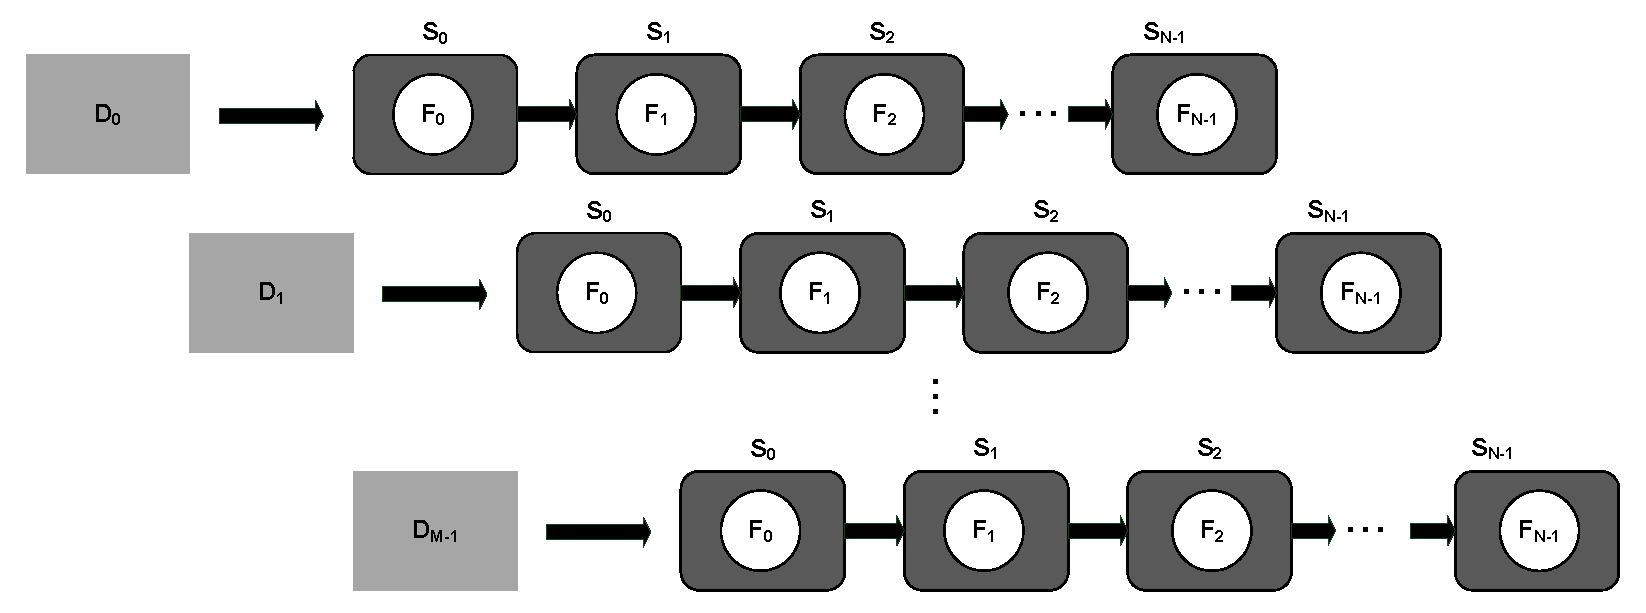
\includegraphics[width= \columnwidth]{Chapter3/figures/skell-pipe}
	\caption{Exemple de squelette du type \textbf{Pipeline}}
	\label{skell-pipe}
\end{figure}
Le parall�lisme r�sulte du fait que l'�valuation des diff�rents fonctions du \textbf{Pipeline} sur des �l�ments diff�rents du flux ($D_{0}$, $D_{1}$ par exemple sur la figure \ref{skell-pipe}) se fait de mani�re ind�pendante. Deux grandeurs caract�risent alors le \textbf{Pipeline} : (1)la latence qui est la dur�e de traitement d'un �l�ment de flux par tous les �tages du pipeline, (2) le d�bit, qui mesure le nombre de r�sultats fournis par unit�s de temps et qui est d�termin� par l'�tage le plus lent du \textbf{Pipeline}.
\subsubsection{Le Squelette Pardo}
Le squelette \textbf{Pardo} permet de placer de mani�re \emph{ad hoc} N fonctions sur N processeurs 
\subsection{Squelettes d�di�s au parall�lisme de donn�es}
\subsubsection{Le Squelette Farm}
\subsubsection{Le squelette SCM}
\subsection{Squelettes d�di�s � la structuration de l�application}
\subsubsection{Le Squelette Sequence}
\subsubsection{Le Squelette Select}

%On trouve dans la litt�rature plusieurs jeux de squelettes algorithmiques r�pondant � divers besoins [45, 22, 5, 88, 119, 54]. Au sein de QUAFF, 
%\section{The Divide \& Conquer Skeleton (Fixed Degree}
%Ce type de squelette provient de la c�l�bre technique du \emph{divide and conquer}. Cette technique peut s'appliquer lorsque la solution � un probl�me peut �tre d�finie r�cursivement comme une collections de sous-probl�mes qui sont des instances plus petites du probl�me original. Les algorithmes de ce type offrent un bon potentiel de parall�lisation. En effet, si l'on arrive � exprimer un probl�me sous forme de sous-probl�mes d�finis r�cursivement  on imagine bien que ces derniers peuvent �tre ex�cut�es de mani�re concurrente sur plusieurs processeurs. L'ex�cution des algorithmes du type \emph{divide and conquer} se r�sume � l'�valuation d'un arbre de processus �voluant dynamiquement, le processus repr�sentant un sous-probl�me g�n�r�. Le d�fi �tant de s'assurer que les d�ploiement de cet arbre virtuel se fait de la mani�re la plus efficace possible sur une vraie machine. 
%\section{The Iterative Combination Skeleton}
%\section{The Cluster Skeleton}
%\section{The Task Queue Skeleton}

%\bibliographystyle{abbrv}
\bibliographystyle{plain}

\bibliography{thesis} 

\end{document}